\documentclass[a4paper,12pt]{article}[abntex2]
\bibliographystyle{abntex2-alf}
\usepackage[table,xcdraw]{xcolor}

% Definições de layout e formatação
\usepackage[a4paper, left=3.0cm, top=3.0cm, bottom=2.0cm, right=2.0cm]{geometry} % Personalização das margens do documento
\usepackage{setspace} % Controle do espaçamento entre linhas
\onehalfspacing % Espaçamento entre linhas de 1,5
\usepackage{indentfirst} % Indentação do primeiro parágrafo das seções
\usepackage{newtxtext} % Substitui a fonte padrão pela Times Roman
\usepackage{titlesec} % Personalização dos títulos de seções
\usepackage{ragged2e} % Melhor controle de justificação do texto
\usepackage[portuguese]{babel} % Adaptação para o português (nomes e hifenização)
\usepackage{amsmath}

% Pacotes de cabeçalho, rodapé e títulos
\usepackage{fancyhdr} % Customização de fcabeçalhos e rodapés
\setlength{\headheight}{14.49998pt} % Altura do cabeçalho
\pagestyle{fancy}
\fancyhf{} % Limpa cabeçalho e rodapé
\rhead{\thepage} % Página no canto direito do cabeçalho

% Pacotes para tabelas
\usepackage{booktabs} % Melhora a qualidade das tabelas
\usepackage{tabularx} % Permite tabelas com larguras de colunas ajustáveis
\usepackage{float} % Melhor controle sobre o posicionamento de figuras e tabelas

% Pacotes para gráficos e imagens
\usepackage{graphicx} % Suporte para inclusão de imagens

\usepackage[utf8]{inputenc}
\usepackage{listingsutf8}

\lstset{
    language=R,                      
    basicstyle=\ttfamily\scalefont{1.0},
    keywordstyle=\color{blue},       
    stringstyle=\color{red},         
    commentstyle=\color{green},      
    numbers=left,                    
    numberstyle=\tiny\color{gray},   
    stepnumber=1,                    
    numbersep=5pt,                   
    backgroundcolor=\color{lightgray!10}, 
    frame=single,                    
    breaklines=true,                 
    captionpos=b,                    
    keepspaces=true,                 
    showspaces=false,                
    showstringspaces=false,          
    showtabs=false,                  
    tabsize=2,
     literate={á}{{\'a}}1
             {é}{{\'e}}1
             {í}{{\'i}}1
             {ó}{{\'o}}1
             {ú}{{\'u}}1
             {Ú}{{\'U}}1
             {â}{{\^a}}1
             {ê}{{\^e}}1
             {î}{{\^i}}1
             {ô}{{\^o}}1
             {û}{{\^u}}1
             {ã}{{\~a}}1
             {õ}{{\~o}}1
             {ç}{{\c{c}}}1,
}


% Pacotes para unidades e formatação numérica
\usepackage{siunitx} % Tipografia de unidades do Sistema Internacional e formatação de números
\sisetup{
  output-decimal-marker = {,},
  inter-unit-product = \ensuremath{{}\cdot{}},
  per-mode = symbol
}
\DeclareSIUnit{\real}{R\$}
\newcommand{\real}[1]{R\$#1}

% Pacotes para hiperlinks e referências
\usepackage{hyperref} % Suporte a hiperlinks
\usepackage{footnotehyper} % Notas de rodapé clicáveis em combinação com hyperref
\hypersetup{
    colorlinks=true,
    linkcolor=black,
    filecolor=magenta,      
    urlcolor=cyan,
    citecolor=black,        
    pdfborder={0 0 0},
}
\makeatletter
\def\@pdfborder{0 0 0} % Remove a borda dos links
\def\@pdfborderstyle{/S/U/W 1} % Estilo da borda dos links
\makeatother

% Pacotes para texto e outros
\usepackage{lipsum} % Geração de texto dummy 'Lorem Ipsum'
\usepackage[normalem]{ulem} % Permite o uso de diferentes tipos de sublinhados sem alterar o \emph{}

\begin{document}

\begin{titlepage}
    \centering
    \vspace*{1cm}
    \Large\textbf{INSPER – INSTITUTO DE ENSINO E PESQUISA}\\
    \Large ECONOMIA\\
    \vspace{1.5cm}
    \Large\textbf{Caderno}\\
    \textbf{Comércio Internacional}\\
    \vspace{1.5cm}
    Prof. Arthur Augusto Viaro\\
    Prof. Auxiliar  \\
    \vfill
    \normalsize
    Hicham Munir Tayfour, \href{mailto:hichamt@al.insper.edu.br}{hichamt@al.insper.edu.br}\\

    \vfill
    São Paulo\\
    Fevereiro/2025
\end{titlepage}

\newpage
\tableofcontents
\thispagestyle{empty} % Esse comando remove a numeração de pagina da tabela de conteúdo

\newpage 
\listoffigures
\thispagestyle{empty} % Esse comando remove a numeração de pagina da tabela de figura

\newpage
\setcounter{page}{1} % Inicia a contagem de páginas a partir desta página
\justify
\onehalfspacing


\section*{\textbf{Programa do Curso}}
\subsection*{\textbf{Motivação}}
Os países são interdependentes e essa interdependência tem se intensificado nas últimas décadas\begin{itemize}
    \item Fluxos migratórios, remessas a seus países natais (remittances)
    \item Fluxos de capitais (financeiro, investimento direto)
    \item Ideias, cultura, idiomas
\end{itemize}

Neste curso, focaremos em um tipo específico de interdependência Comércio de bens e serviços

\subsection*{\textbf{Principais questões}}
\begin{itemize}
    \item Por que os países fazem comércio?
    \item Explorar diferenças entre eles\begin{itemize}
        \item Tecnologia: Modelo Ricardiano
        \item Dotações de fatores: Modelo de Heckscher-Ohlin
    \end{itemize}
    \item Acessar uma maior variedade de produtos \begin{itemize}
        \item Modelos de Economias de Escala (Krugman)
    \end{itemize}
    \item  Eficiência: Comércio é bom para a economia como um todo? \begin{itemize}
        \item Ganhos de troca
        \item Avaliar o efeito líquido de ganhos e perdas
        \item Acesso a uma maior variedade de produtos
    \end{itemize}
    \item Distribuição de renda\begin{itemize}
        \item Quem são os vencedores e perdedores?
    \end{itemize}
    \item Quais são os impactos da política comercial?
    \item     Quais as motivações por trás de políticas protecionistas?
\end{itemize}

\subsection*{\textbf{Estrutura do Curso}}

\begin{enumerate}
    \item Introdução
    \item Equilíbrio Geral\begin{itemize}
        \item Economia de trocas
        \item Economia com produção
    \end{itemize}
    \item Teoria do Comércio Internacional\begin{itemize}
        \item Diferenças Tecnológicas: Modelo Ricardiano
        \item Dotações de Fatores: Modelo de Heckscher-Ohlin
        \item Curto Prazo vs Longo Prazo: Modelo de Fatores Específicos
        \item Economias de Escala I: Comércio Intraindústria
        \item Economias de Escala II: Indústria Nascente
    \end{itemize}
    \item Política Comercial\begin{itemize}
        \item Política Comercial e Análise de Bem-Estar
        \item Política Comercial Estratégica
    \end{itemize}
\end{enumerate}

\subsection*{\textbf{Pré-Requisitos}}
\begin{itemize}
    \item Conceitos básicos de cálculo\begin{itemize}
        \item Derivadas
        \item Otimizações
    \end{itemize}
    \item Conceitos de Microeconomia\begin{itemize}
        \item Teoria do consumidor
        \item Teoria da firma
        \item Equilíbrio parcial
    \end{itemize}
\end{itemize}

\subsection*{\textbf{Avaliações}}
\begin{itemize}
    \item \textbf{Quiz}: 15\% da média final \begin{itemize}
        \item 4 quizzes com 1 descarte
        \item 21/fev, 14/mar, 30/abr, 23/mai
    \end{itemize}
    \item \textbf{APS}: 10\% da média final
    \item \textbf{PI}: 30\% da média final
    \item \textbf{PF}: 45\% da média final
\end{itemize}
\newpage

\section{\textbf{Introdução}}
\subsection{\textbf{Duas Ondas de Globalização}}

\begin{figure}[H]
    \centering
    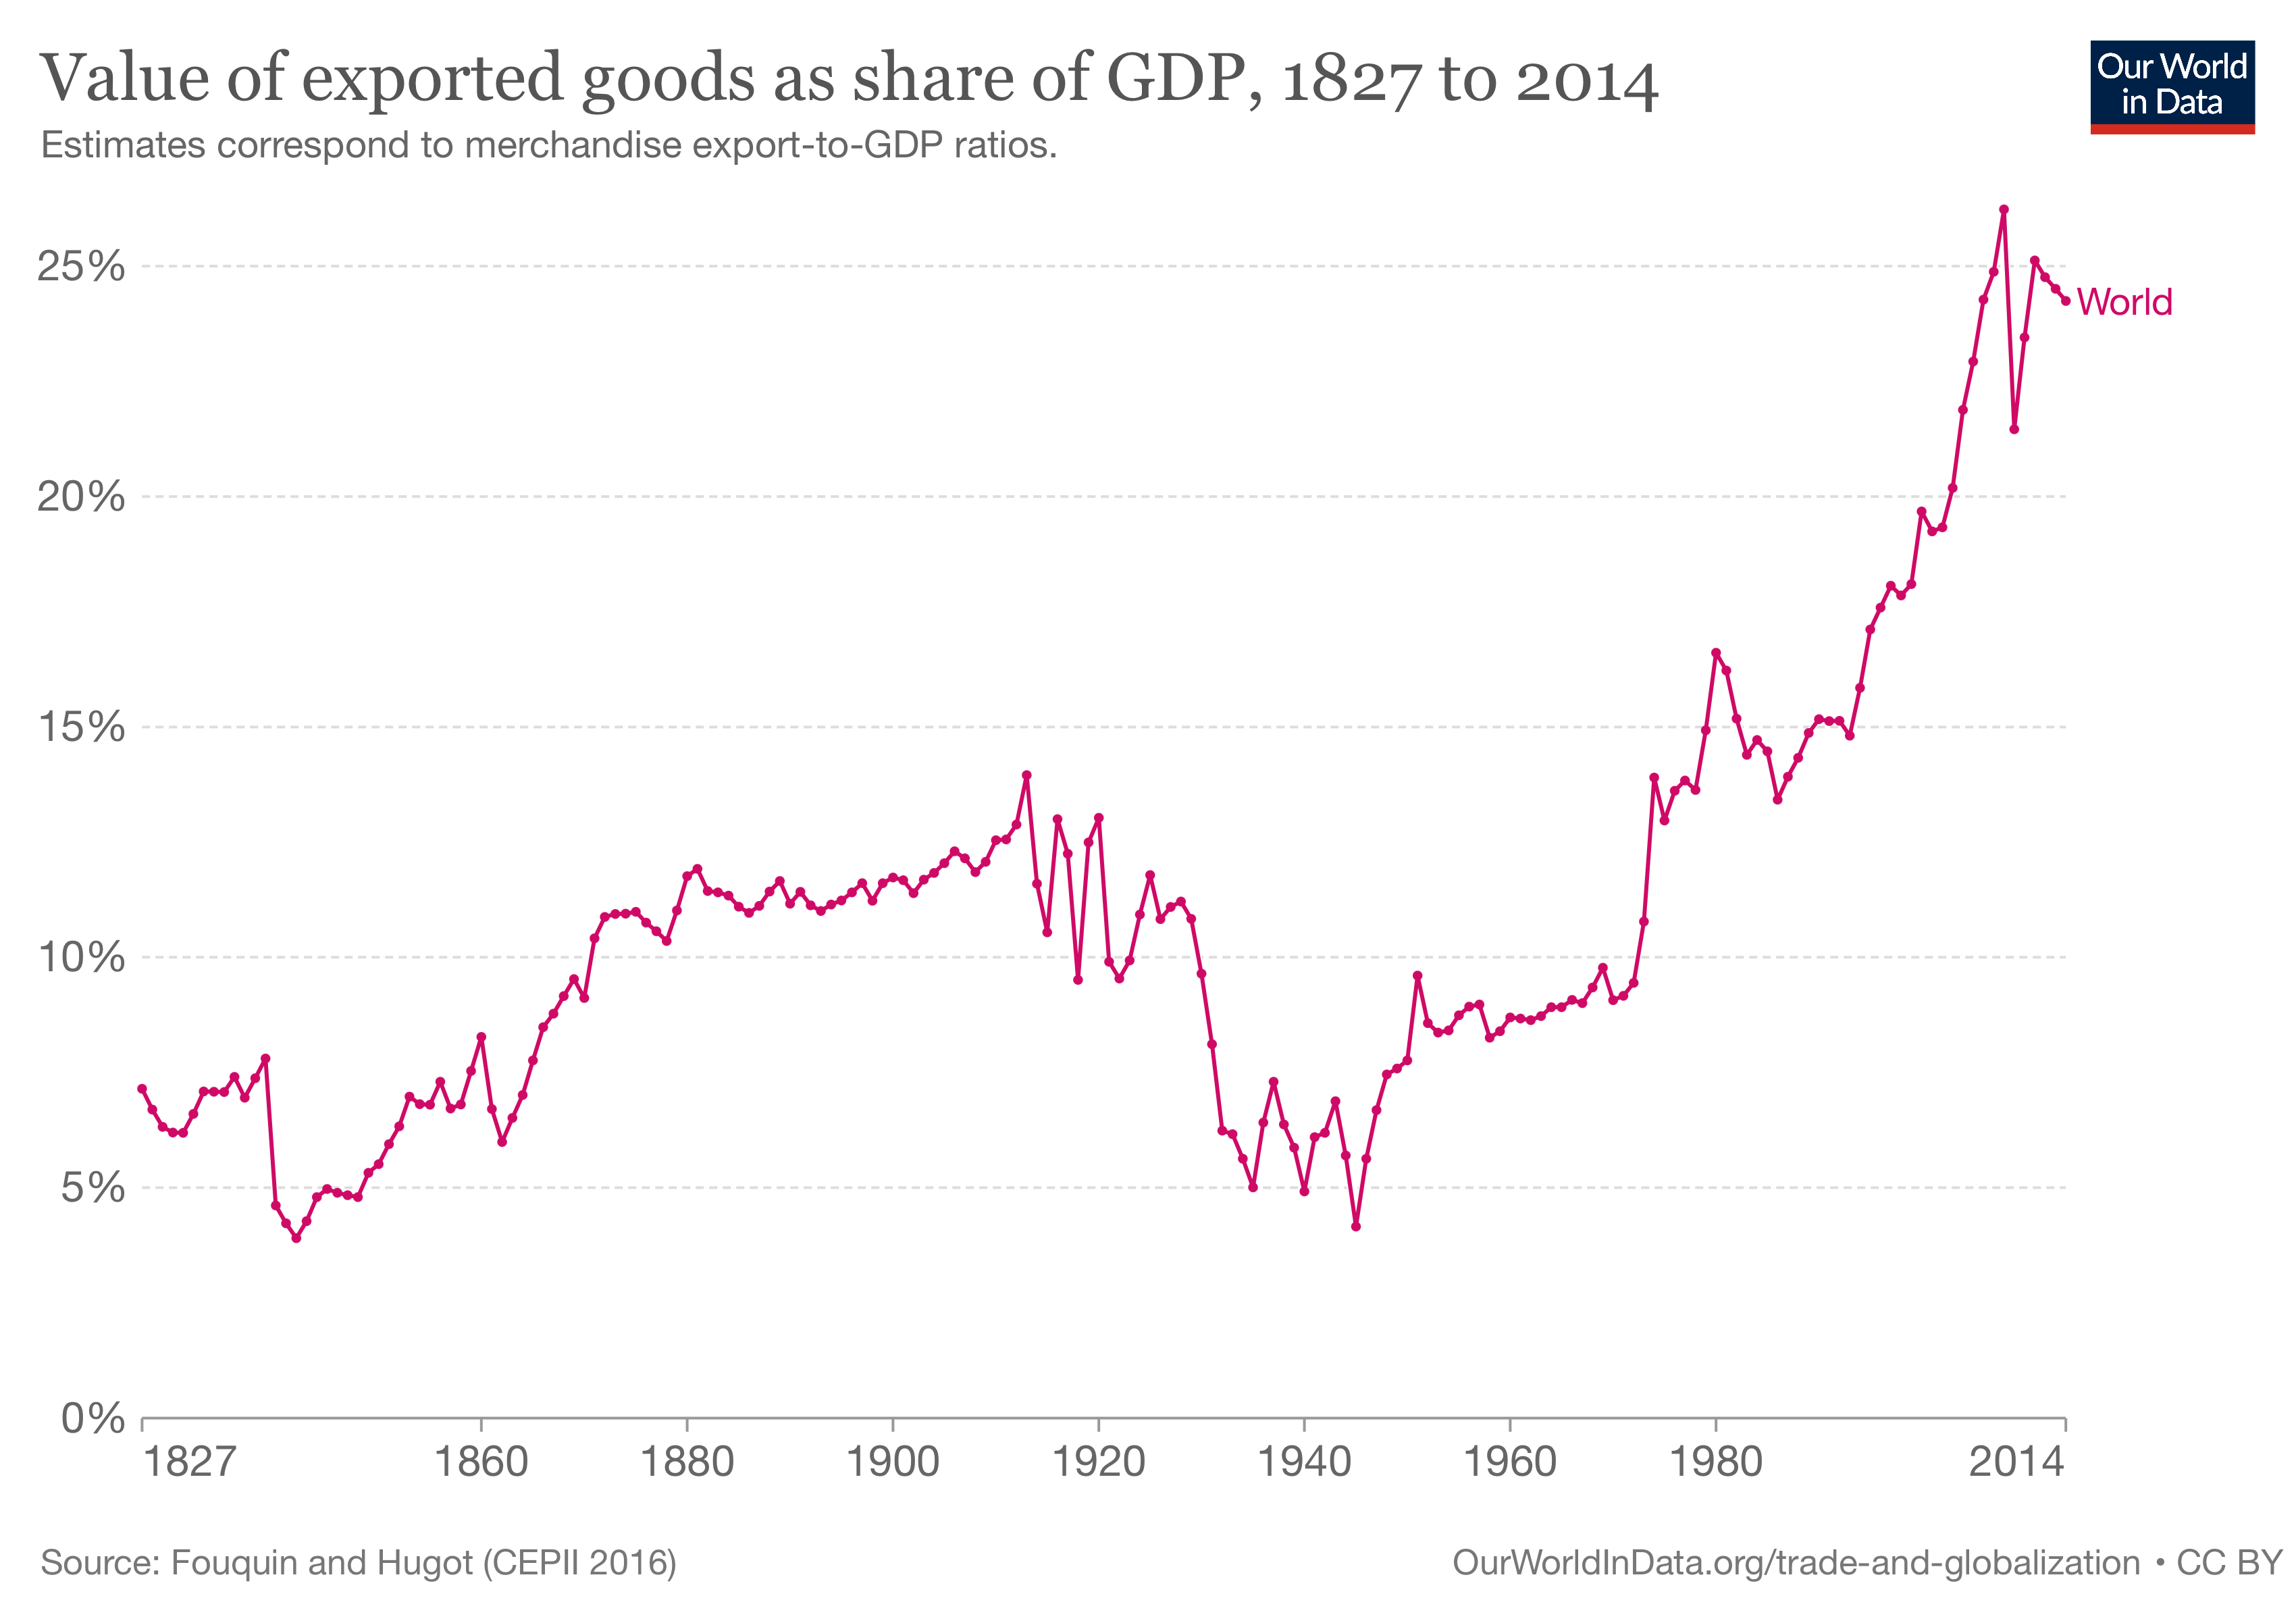
\includegraphics[width=0.70\linewidth]{Imagens/a1i1.png}
\end{figure}

\begin{figure}[H]
    \centering
    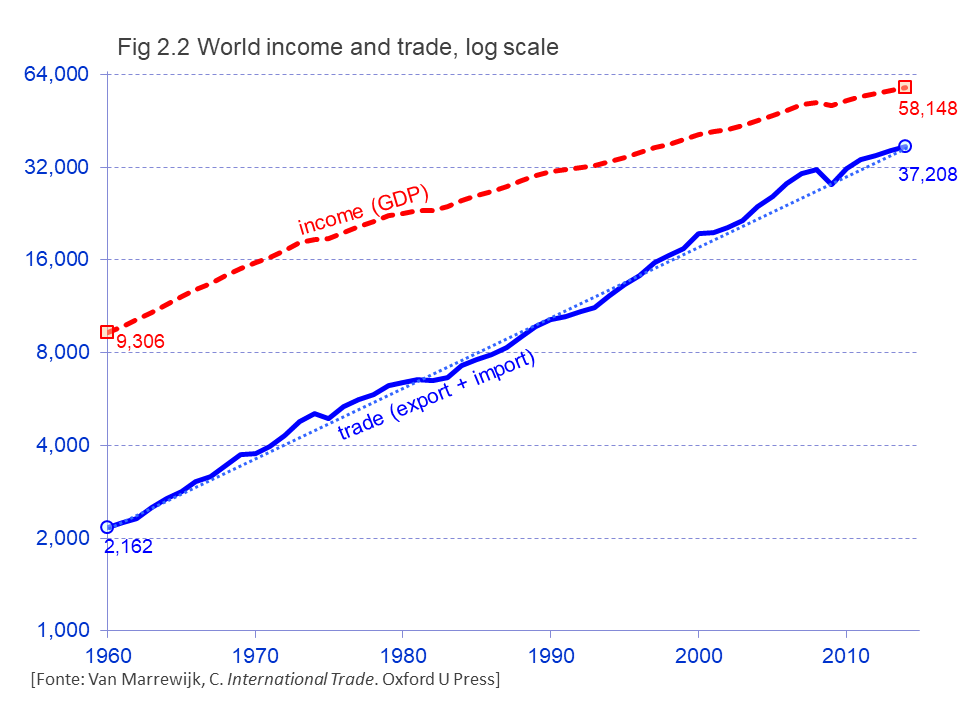
\includegraphics[width=0.70\linewidth]{Imagens/a1i2.png}
\end{figure}

PIB 2014/PIB 1960 = 6,2x (+3,4\% a.a. em média)

Comércio 2014/Comércio 1960 = 17,2x (+5,3\% a.a., em média)

\begin{figure}[H]
    \centering
    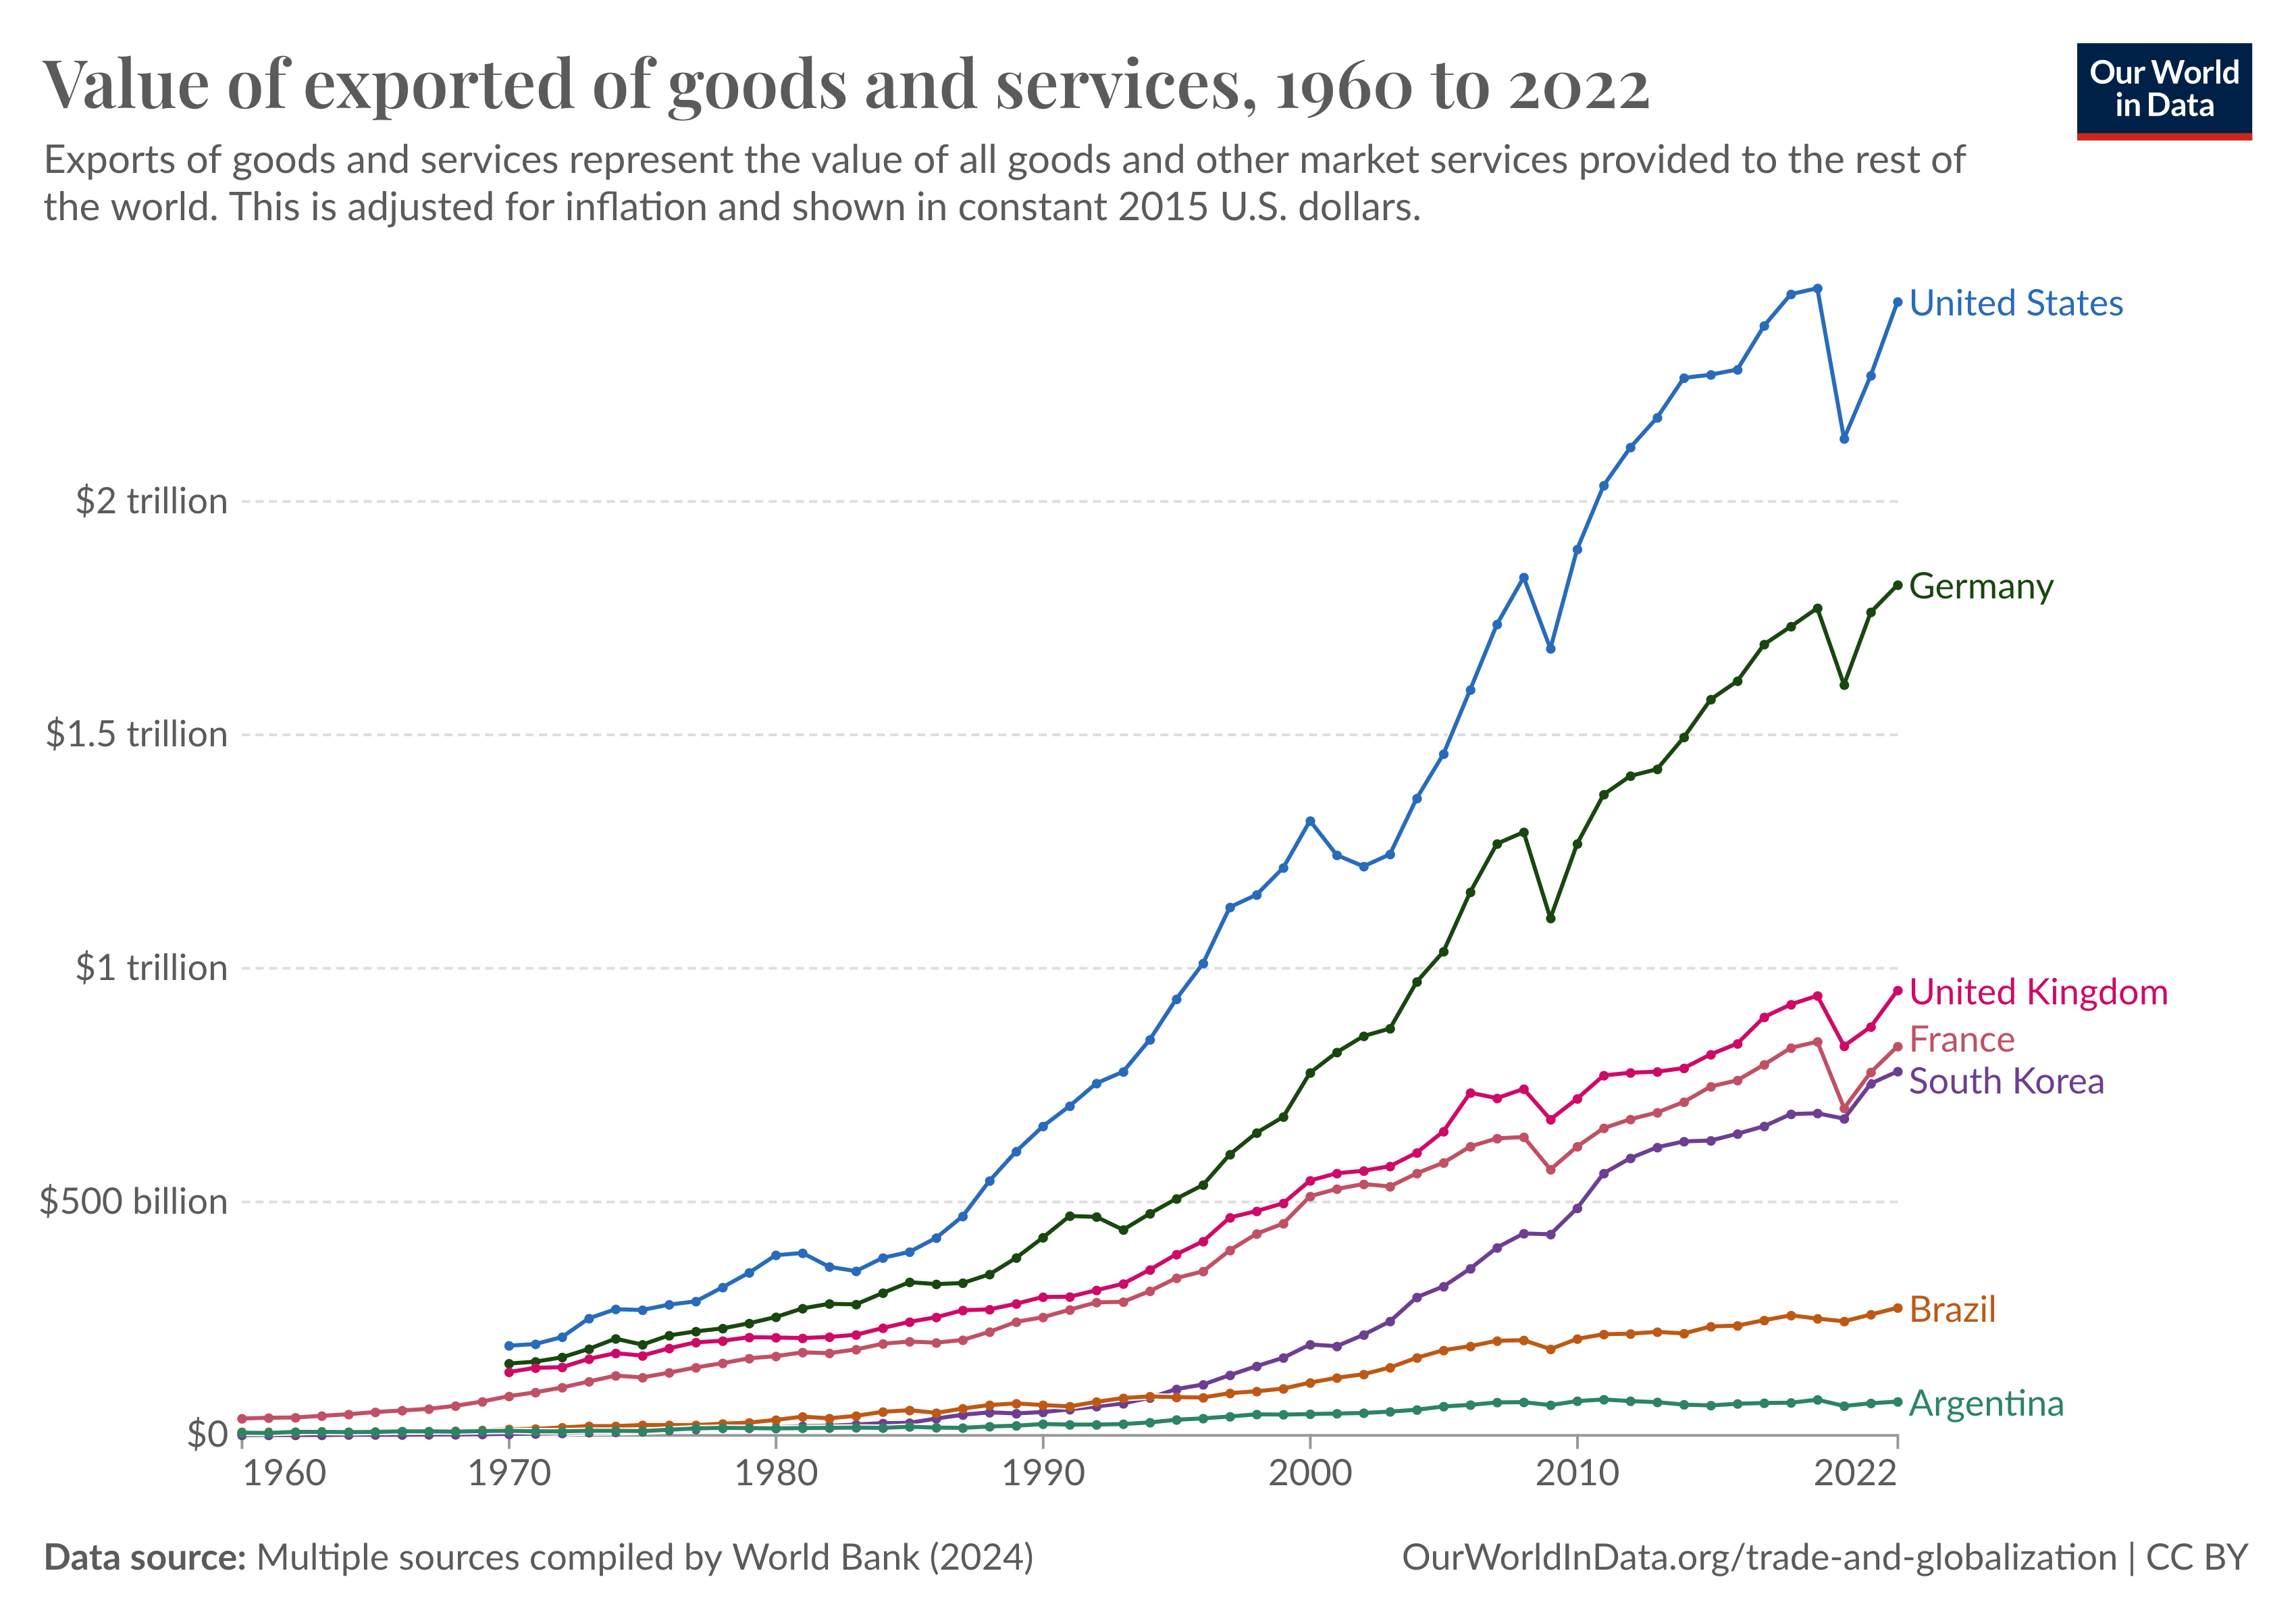
\includegraphics[width=0.70\linewidth]{Imagens/a1i3.png}
\end{figure}

Os países têm reduzido suas barreiras ao comércio\begin{itemize}
    \item Tarifas, quotas, subsídios etc.
    \item WTO, acordos bilaterais, blocos econômicos
    \item Países grandes se abriram ao comércio (China, Índia)
\end{itemize}

Tecnologia reduz custos de transporte e comunicação \begin{itemize}
    \item Navios maiores e mais rápidos, aviação
    \item Refrigeração
    \item Telecomunicações, Internet
    \item Fragmentação da produção
\end{itemize}

\subsubsection{\textbf{Avanço Tecnológico}}
\begin{figure}[H]
    \centering
    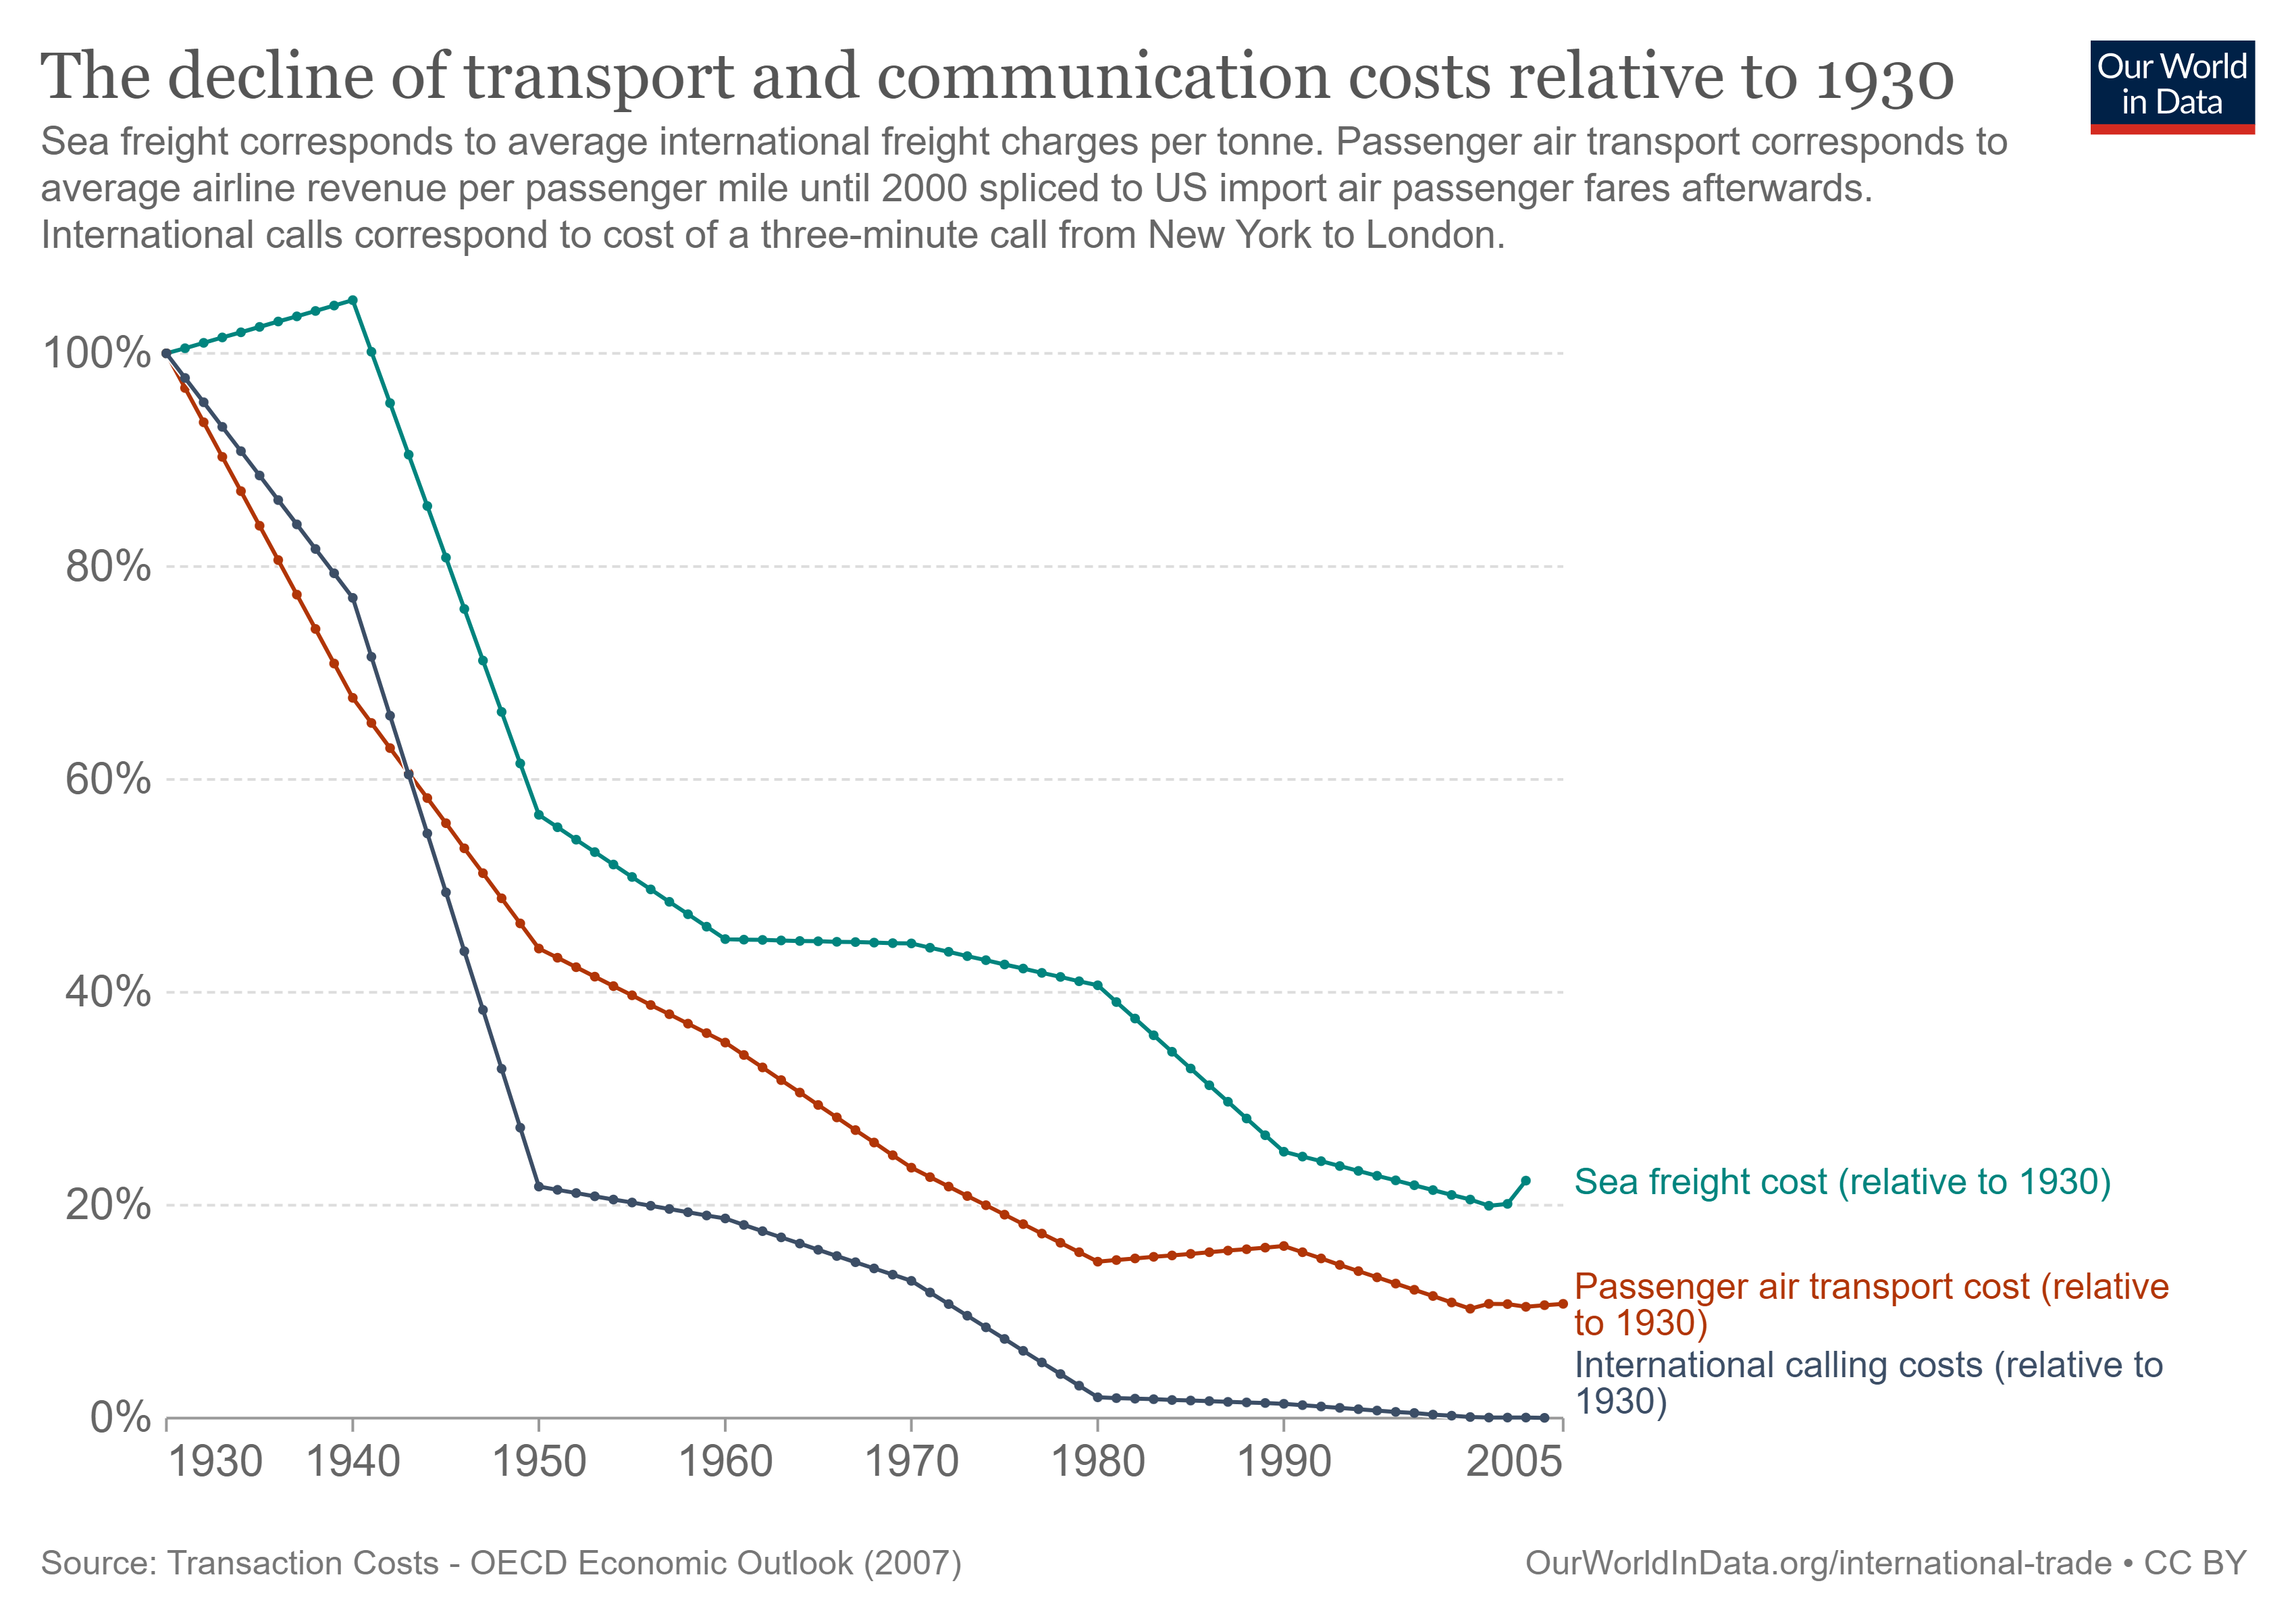
\includegraphics[width=0.70\linewidth]{Imagens/a1i4.png}
\end{figure}

\begin{figure}[H]
    \centering
    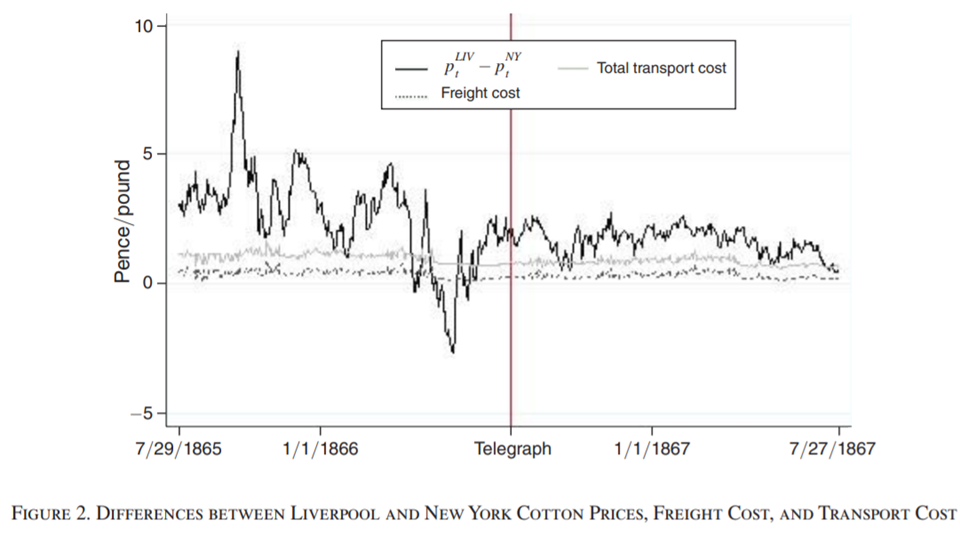
\includegraphics[width=0.70\linewidth]{Imagens/a1i5.png}
\end{figure}

\subsubsection{\textbf{Redução Tarifas}}
\begin{figure}[H]
    \centering
    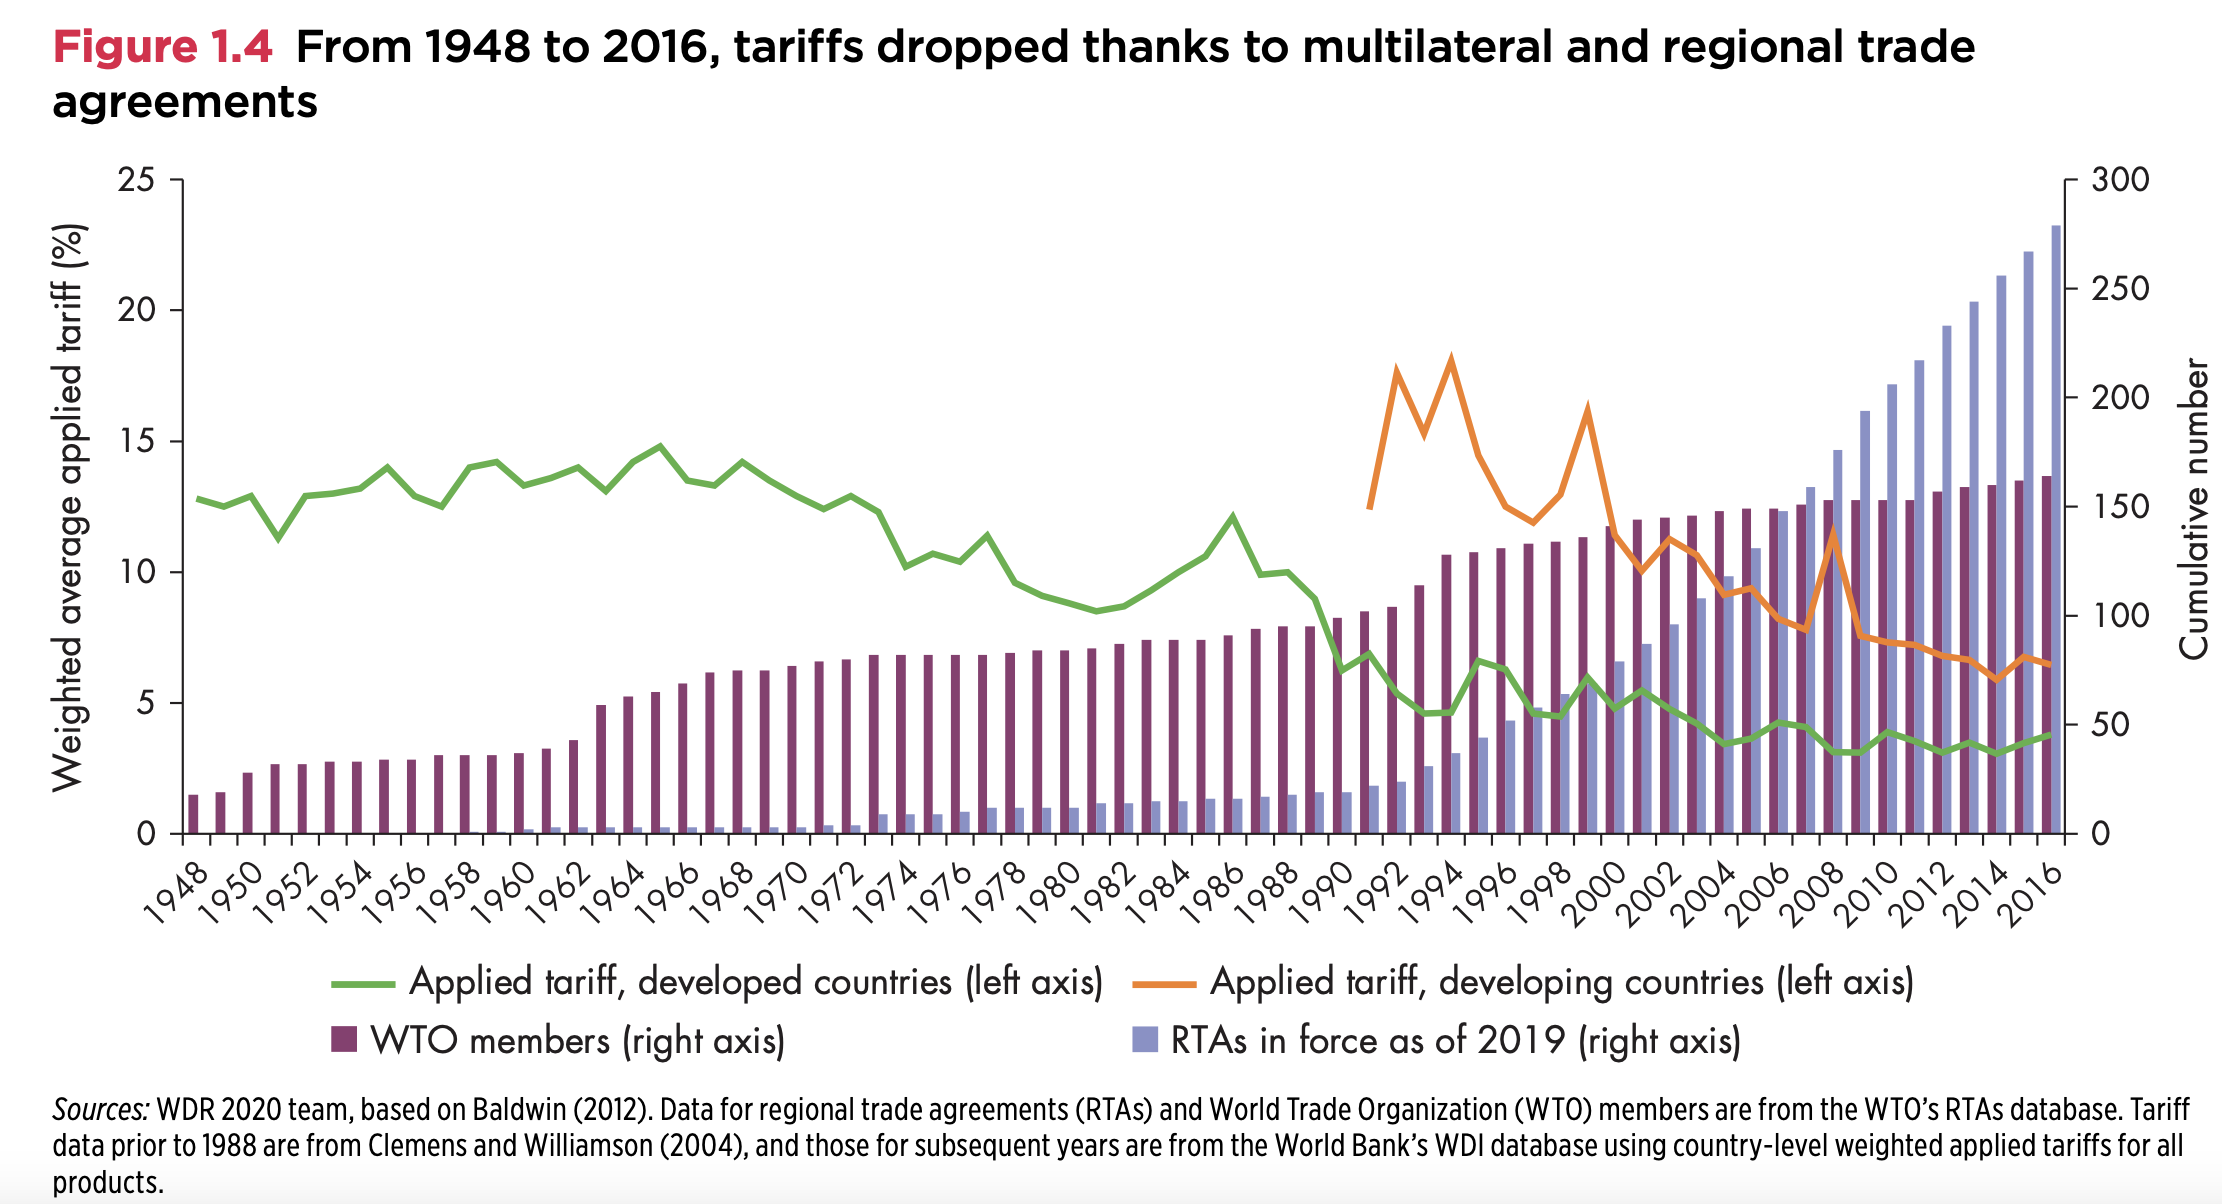
\includegraphics[width=0.70\linewidth]{Imagens/a1i6.png}
\end{figure}

\subsubsection{\textbf{Cadeias Globais de Valor}}
\begin{figure}[H]
    \centering
    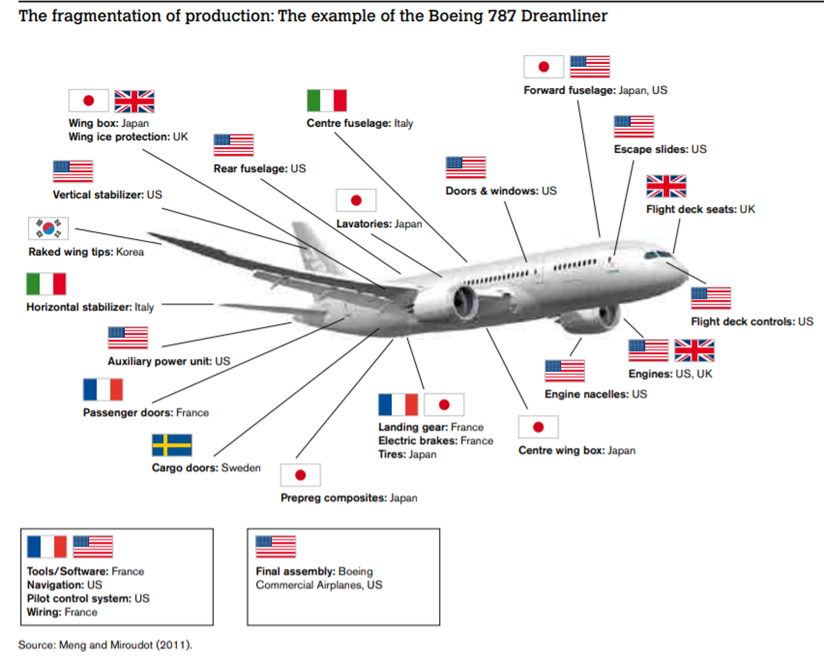
\includegraphics[width=0.70\linewidth]{Imagens/a1i7.png}
\end{figure}
O comércio de bens intermediários se fragmentou, onde cada parte do globo produz uma parte do produto final e depois elas se unem para a criação do bem final. 
\subsection{\textbf{Mapa de Comércio}}
\subsubsection{\textbf{Principais Países}}
\begin{itemize}
    \item Quais países comercializam mais?
    \item O tamanho da economia é diretamente proporcional ao volume de exportações e importações\begin{itemize}
        \item Economias maiores produzem mais bens e serviços para vender no mercado
        \item Economias maiores geram mais renda de bens e serviços vendidos, portanto, são capazes de importar mais
    \end{itemize}
\end{itemize}

\begin{figure}[H]
    \centering
    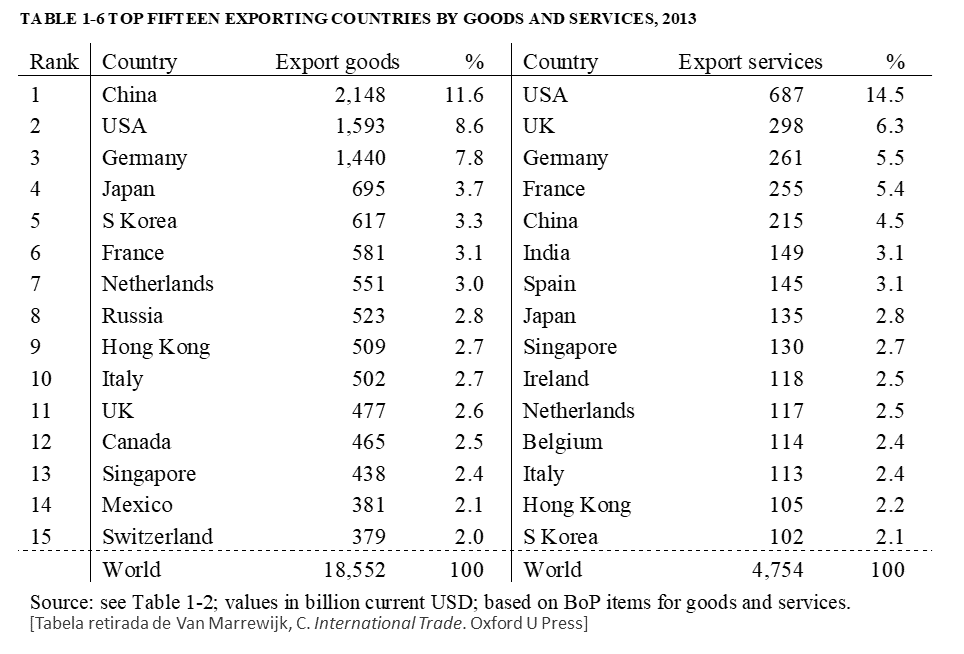
\includegraphics[width=0.70\linewidth]{Imagens/a1i8.png}
\end{figure}

Tamanho parece que importa, e além disso, a relação de importação e exportação , na maioria dos casos, é de um pra um.

\begin{figure}
    \centering
    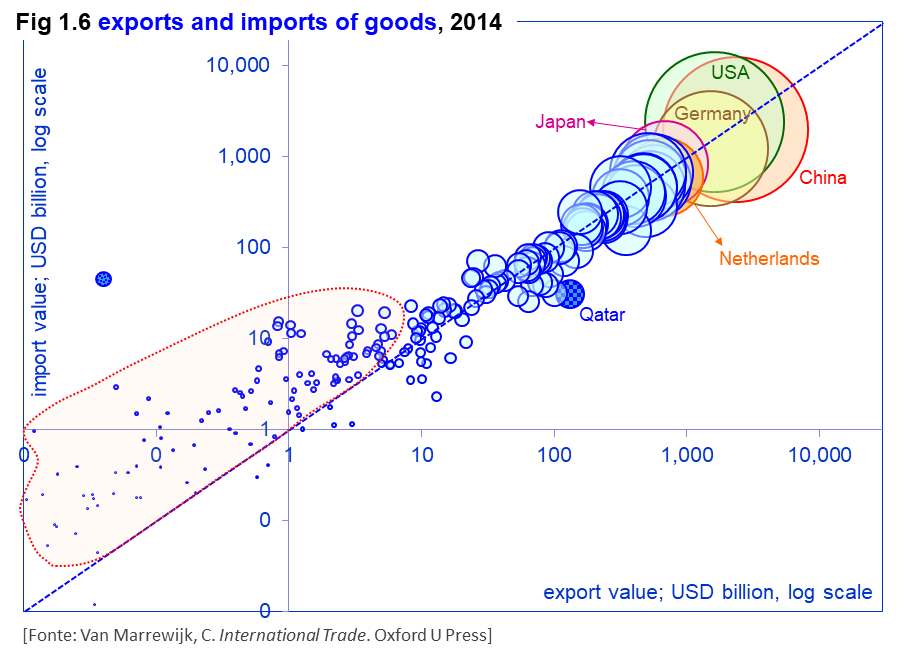
\includegraphics[width=0.70\linewidth]{Imagens/a1i9.png}
\end{figure}

Como proporção do PIB a relação é inversa (países menores fazem mais comércio)
\begin{figure}[H]
    \centering
    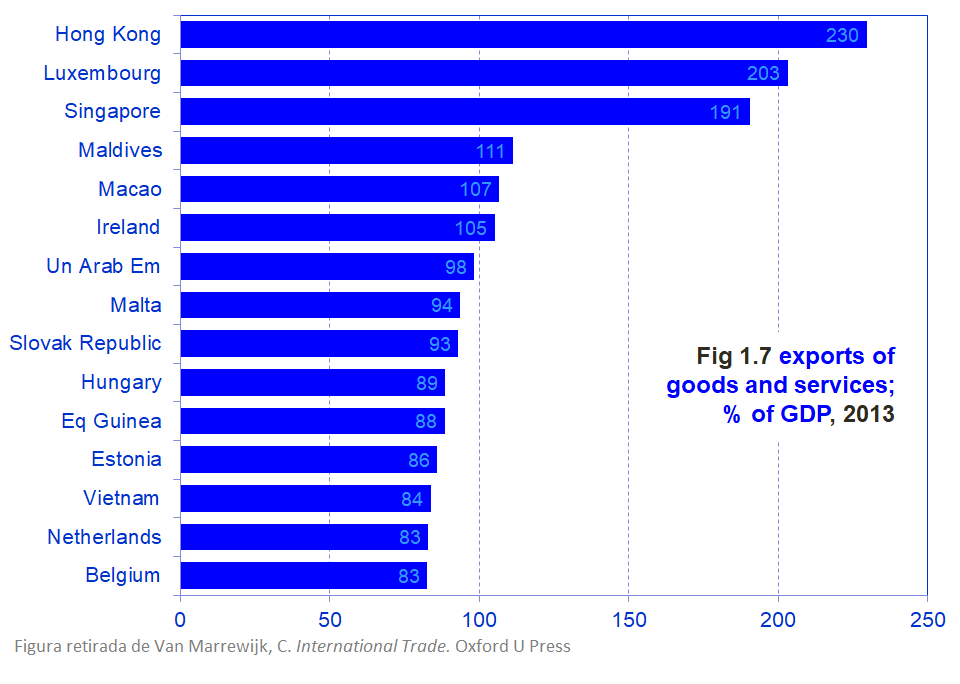
\includegraphics[width=0.70\linewidth]{Imagens/a1i16.png}
\end{figure}
Países pequenos não conseguem produzir tudo que precisam, por isso é difícil deles se fecharem, por isso eles dependem muito do comércio, e o ganho gerado pela abertura comercial é muito grande, em comparação ao seu fechamento.

\subsection{\textbf{Teorias de Comércio Internacional}}
\subsubsection{\textbf{Explicando o Padrão de Comércio}}
\textbf{Vantagens Comparativas}

\begin{figure}[H]
    \centering
     \caption{Net exports and price changes for 1869, Japan – Figure 4 in Bernhofen and Brown (2014)}
    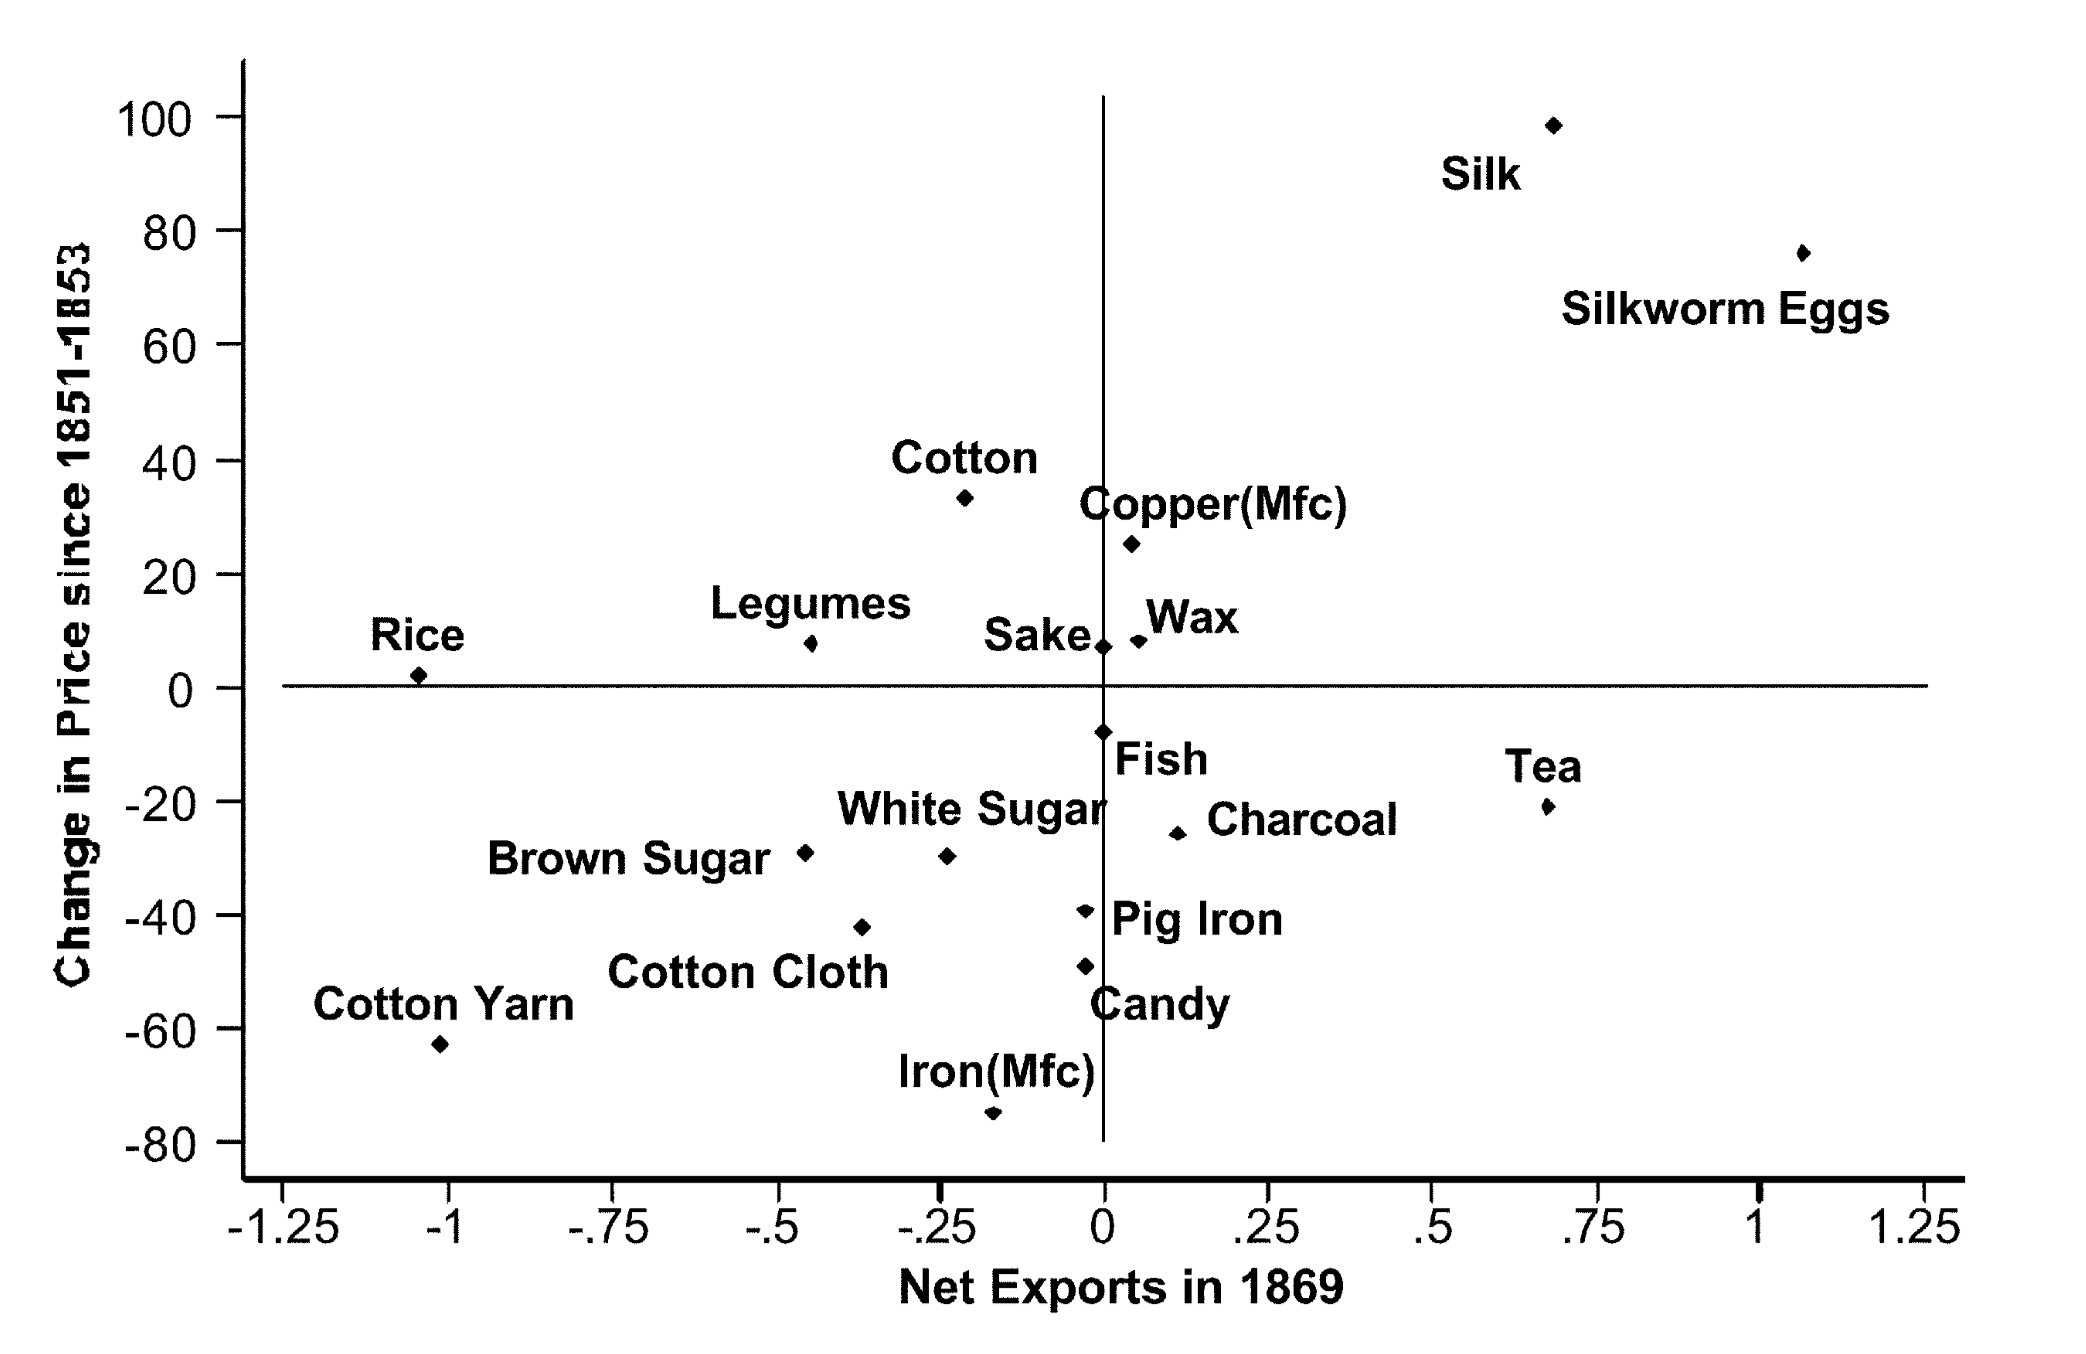
\includegraphics[width=0.70\linewidth]{Imagens/a1i10.png}
\end{figure}
Por que é bom fazer comércio? Parece ser bom. Mas teoricamente, como explicar suas relações comercias, o que ele vai exportar e o que importar ?

Na teoria do comércio clássica, a teoria das vantagens comparativas explica isso, países com vantagens de produzir, de maneira mais barata, um bem em relação aos outras países. Mas só isso explica? Isso é uma verdade absoluta?

Veremos modelos que detalham os resultados sobre preços de produtos de bens de países com vantagem comparativa(o bem da vantagem comparativa(o exportado) vai ficar mais caro no país, enquanto o bem importado vai ficar mais barato no país)

\subsubsection{\textbf{Economias de Escala}}
\begin{figure}[H]
    \centering
    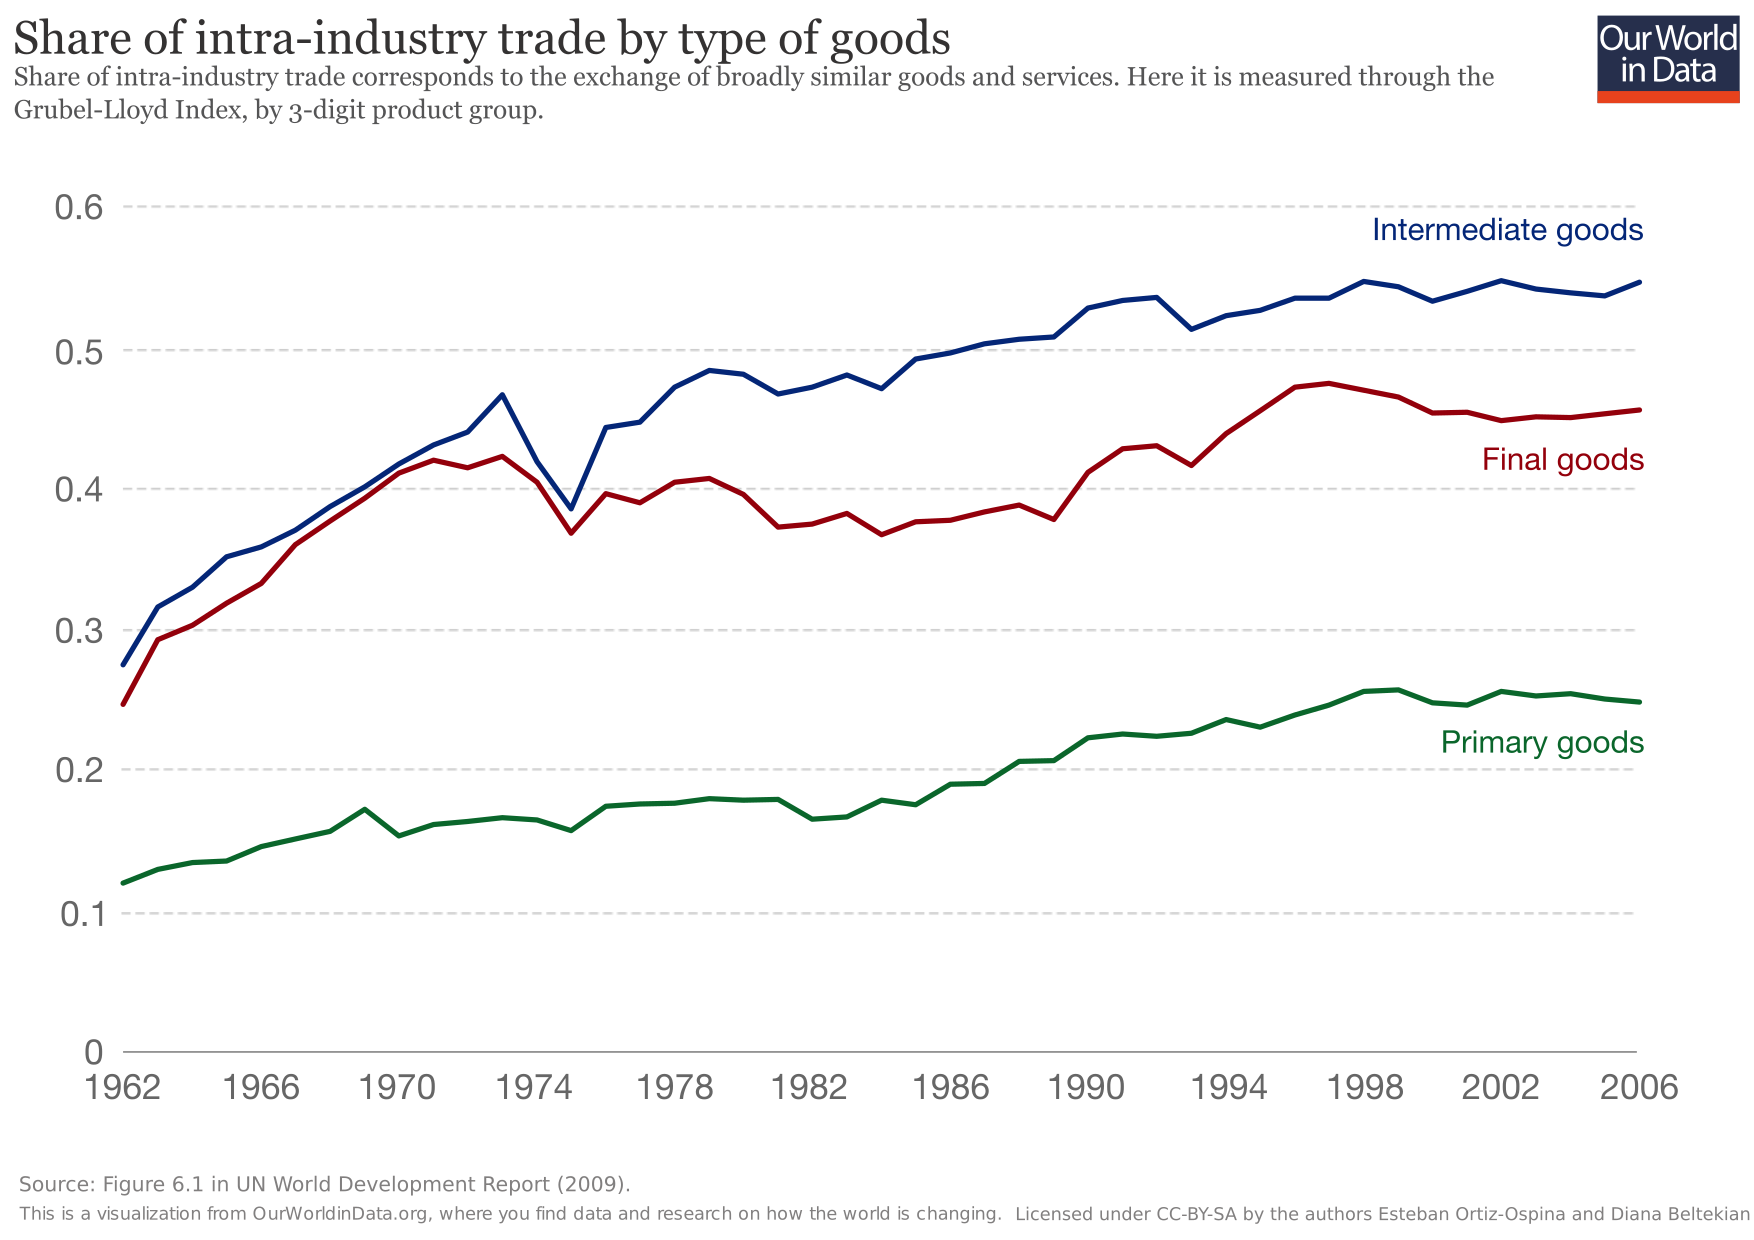
\includegraphics[width=0.70\linewidth]{Imagens/a1i11.png}
\end{figure}

\begin{figure}[H]
    \centering
    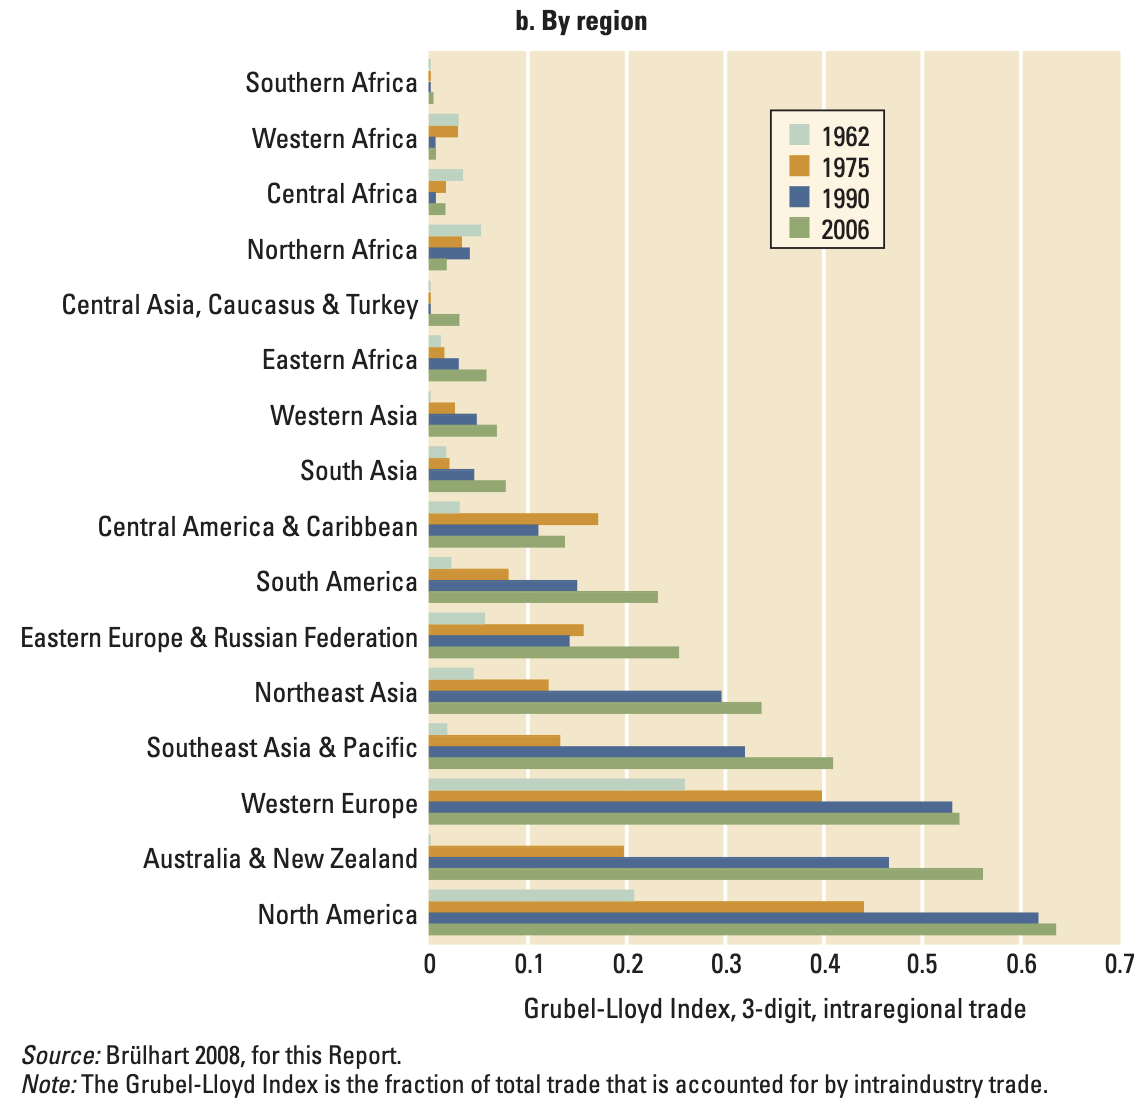
\includegraphics[width=0.70\linewidth]{Imagens/a1i12.png}
\end{figure}

Aqui veremos um furo na teoria, pois aqui países muitos são muito parecidos em termos tecnológicos, apesar da vantagem comparativa, ele importa bens que ele exporta. Algo que a teoria do comércio clássica não é capaz de explicar.

Já que, por exemplo, a França exporta vinhos, mas importa vinhos chilenos, apesar de ser \textbf{vinho}, é um outro tipo de vinho, assim que a população enxerga.

Mas só se abrir comércio gera crescimento? Mas crescer não aumenta comércio? É uma relação de sentido duplo? Há alguma variável secundária que gera ambos? 

\subsection{\textbf{Consequências do Comércio Internacional}}
\subsubsection{\textbf{Quais as consequências do comércio internacional para as economias?}}
\begin{figure}
    \centering
    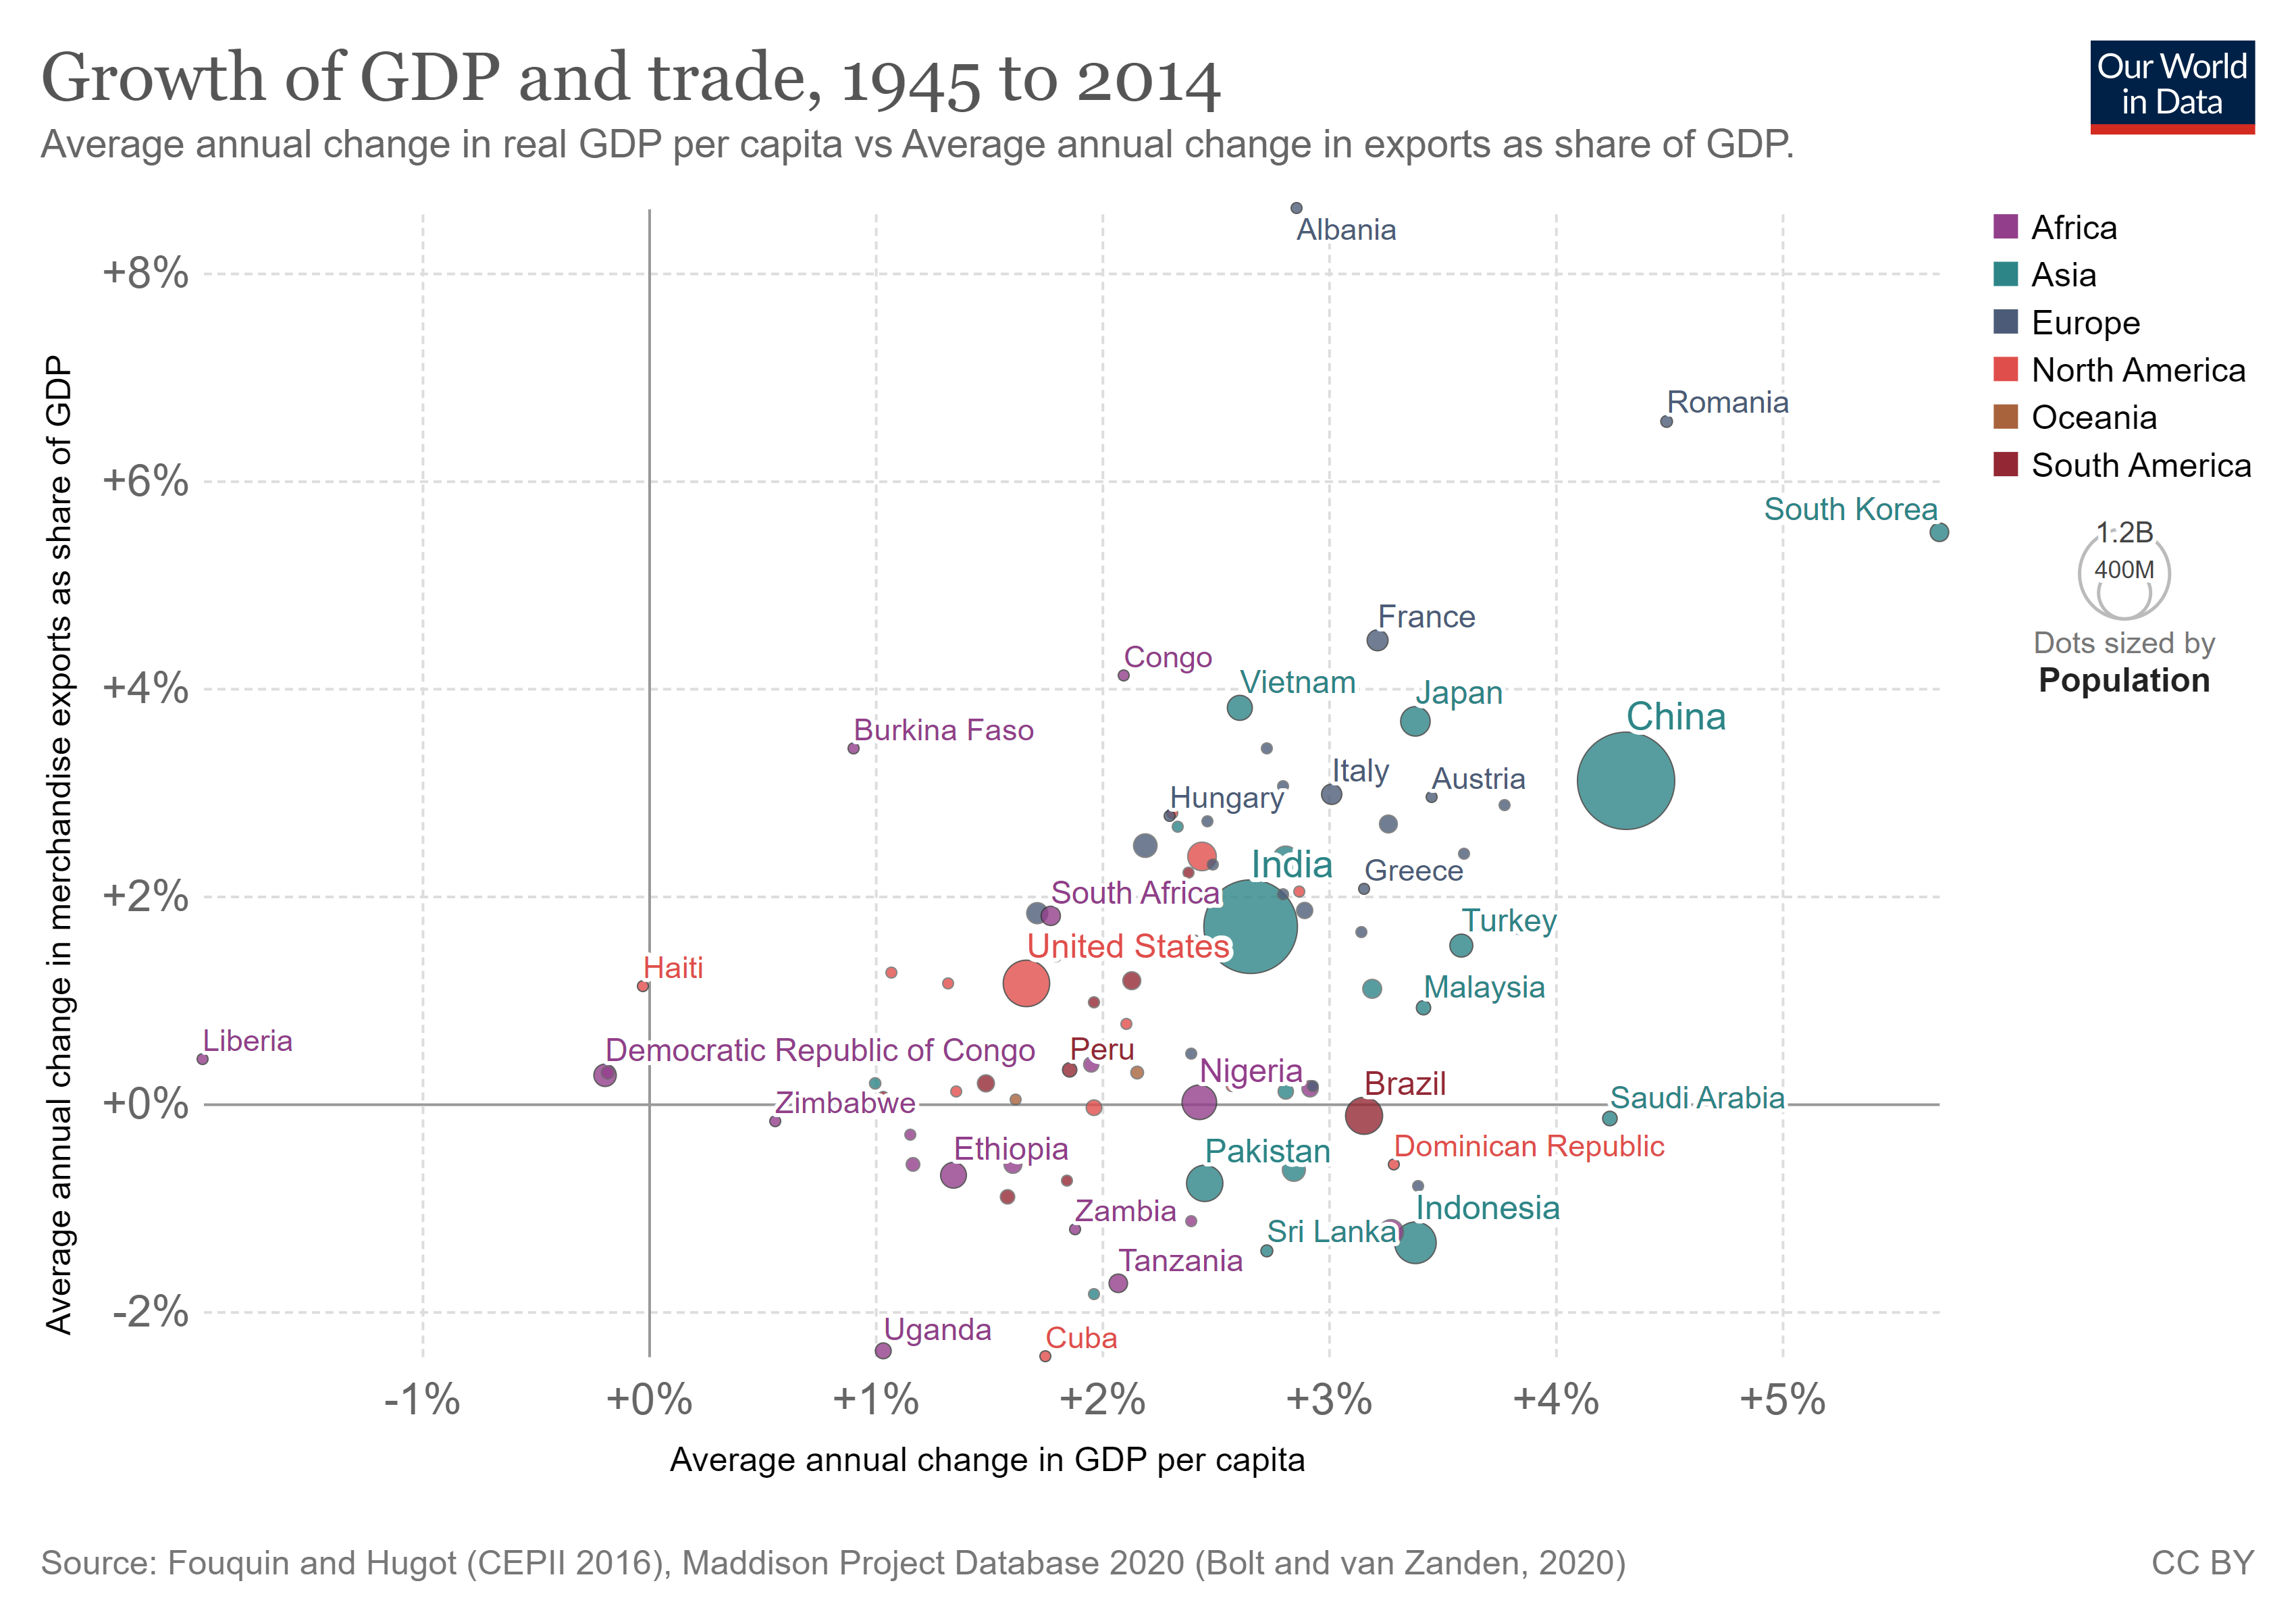
\includegraphics[width=0.70\linewidth]{Imagens/a1i13.png}
\end{figure}

\subsubsection{\textbf{Crescimento Econômico}}
Associação Positiva entre Crescimento Econômico e Comércio é Causal?

Potenciais Mecanismos
\begin{itemize}
    \item Aumento da competição
    \item Economias de escala
    \item Aprendizado e inovação
\end{itemize}

Em geral, a evidência empírica sugere que o comércio melhora a eficiência da economia. Mas ainda há muita coisa a ser descoberta em relação as causalidades de desenvolvimento.

Estes resultados são importantes, pois mostram que há ganhos com o comércio.

\subsubsection{\textbf{Efeitos Distributivos}}
Então, por que os países continuam adotando políticas comerciais para proteger suas indústrias da competição internacional?

O comércio possui consequências distributivas relevantes\begin{itemize}
    \item Nem todo mundo se beneficia da mesma maneira
    \item Efeitos de \textbf{equilíbrio geral}
\end{itemize}

A distribuição dos ganhos depende da cesta de consumo e do tipo de trabalho dos diferentes grupos de pessoas

\begin{figure}[H]
    \centering
    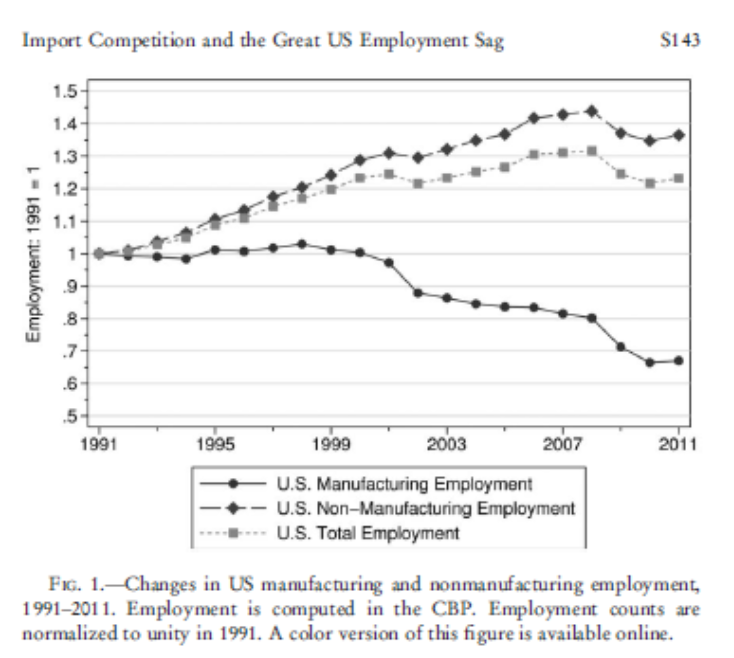
\includegraphics[width=0.70\linewidth]{Imagens/a1i14.png}
\end{figure}

\begin{figure}[H]
    \centering
    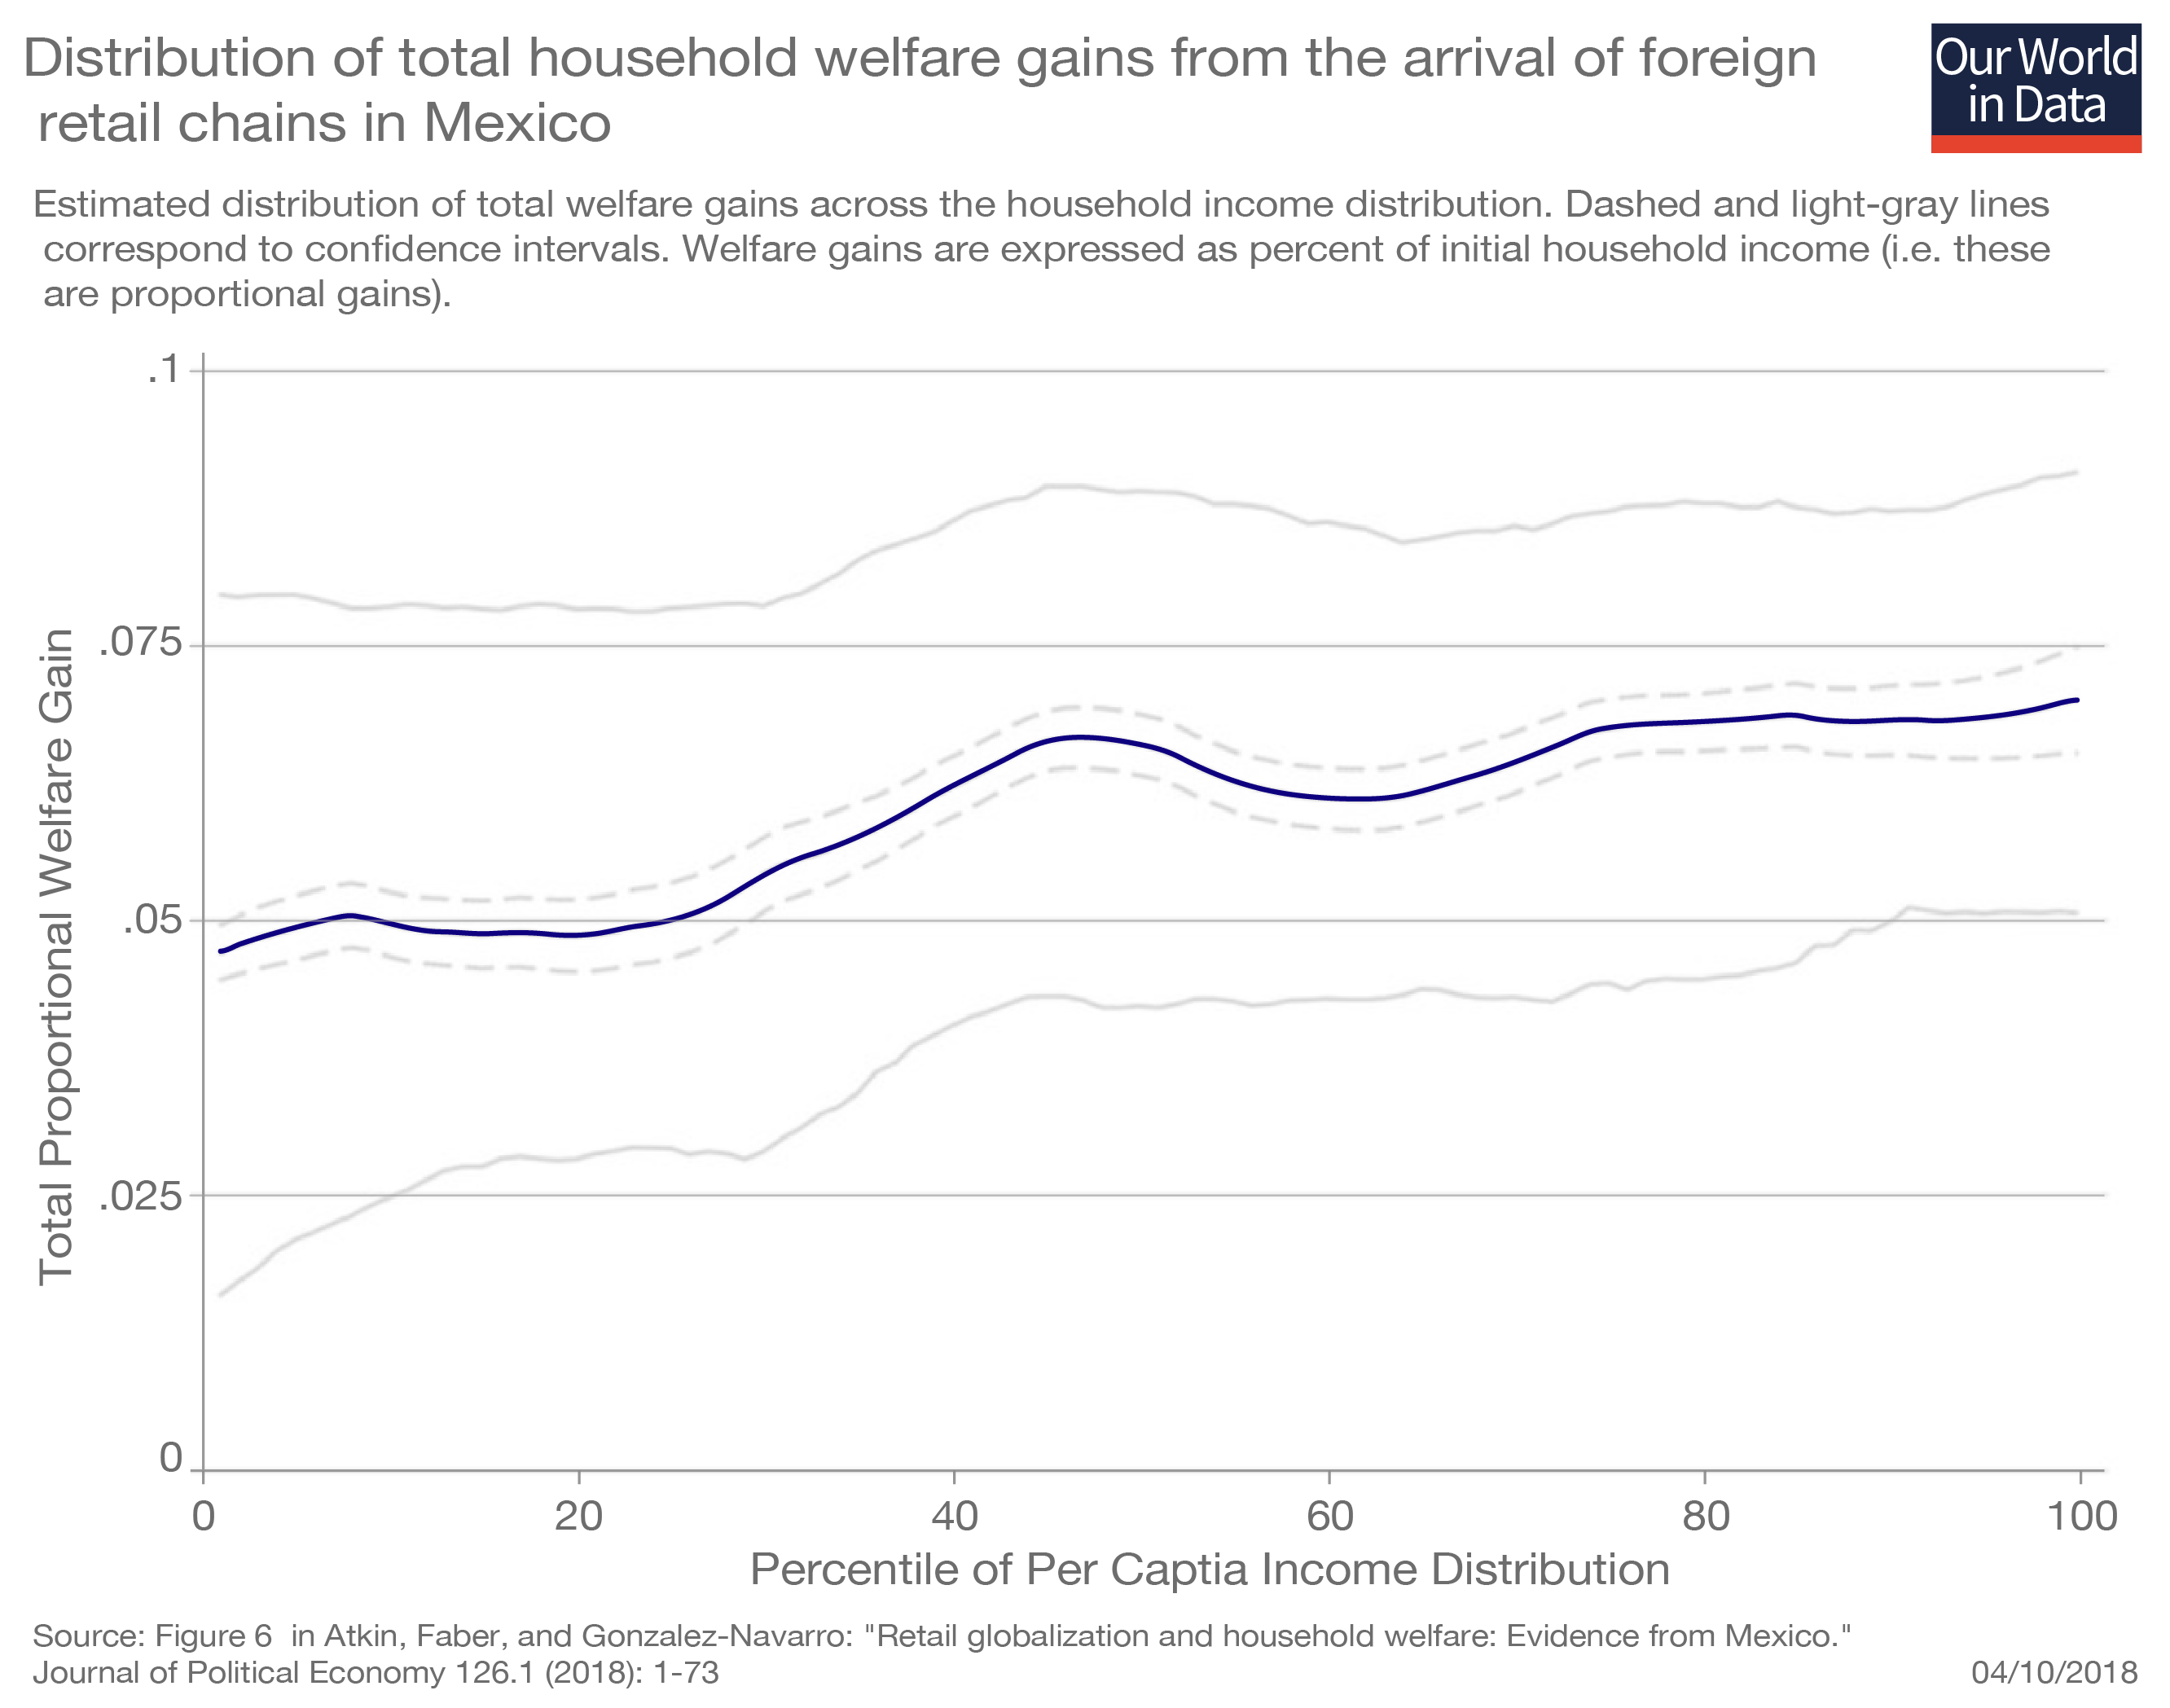
\includegraphics[width=0.70\linewidth]{Imagens/a1i15.png}
\end{figure}
Nem todos são afetados da mesma forma, Wallmart entrou no México fazendo o custo de vida caiu, mas todo o setor varejista perdeu. Esse é um resulto do poder distributivo do comércio. 
\newpage

\section{\textbf{Equilíbrio Geral: Economia de Trocas}}
\subsection{\textbf{Motivação}}
\textit{\textbf{Países Avançados podem ganhar comercializando com países Emergentes?}}
\begin{itemize}
    \item Pode até ser uma pergunta simples, mas podemos tirar muitas coisas em relação a ela 
    \item Estamos usando dois países muito distintos, avançados e emergentes(EUA e Cuba(ou grande parte dos outras países do globo)), esse tipo de comércio gera ganhos(em termos de bem estar) para ambos para os países
\end{itemize}
Até agora, estudamos o mercado de um único bem isolado, chamamos esse estudo de um único mercado damos o nome de equilíbrio parcial, pouco importa o que acontece em outros setores, independente se eles são correlacionados (é como se o mercado de carro fosse independente do mercado de aço).

Embora seja muito útil, esse tipo de modelo está bem distante da realidade, pois os mercados estão interligados\begin{itemize}
    \item Aumento na oferta de açúcar\begin{itemize}
        \item reduz preços do açúcar
        \item queda do emprego nas fazendas de cana-de-açúcar
        \item maior oferta de trabalhadores reduz os salários no campo 
        \item menor produção de cana eleva a disponibilidade de terra 
        \item aumento na produção de outras culturas
        \item preços dos alimentos diminuem
        \item renda real dos consumidores aumenta
        \item renda maior eleva a demanda por viagens internacionais 
        \item não há fim para essa sequência de eventos
        \end{itemize}
    \end{itemize}

Vemos que a realidade é muito mais complexa do que imaginamos, um mundo deixa de ser "unidimensional" e agora parece que os mercados estão em uma rede interligada, para isso começaremos a olhar em preços relativos.

O exemplo nos mostra que, em um certo sentido, não existe um mercado de um único bem

Todas as mudanças nas quantidades ou preços afetam a demanda e/ou oferta de outros bens\begin{itemize}
    \item Efeitos na renda
    \item Substituibilidade ou complementariedade de bens
    \item Abundância ou escassez de recursos
\end{itemize}

Precisamos, portanto, de um modelo que acomode as interações \textbf{entre todos os mercados simultaneamente}.

\subsection{\textbf{Hipótese}}

Na próximas aulas, vamos analisar um modelo de \textbf{equilíbrio geral} em contraposição aos modelos de \textbf{equilíbrio parcial} estudados até agora. Lembrando que o equilíbrio geral traz uma complexada muito grande quanto mais mercados estão envolvidos

Por se tratar de um problema complexo, vamos adotar algumas simplificações para tornar o problema analiticamente tratável:
\begin{itemize}
    \item Mercados competitivos, todos os a gentes econômicos são tomadores de preços, ninguém sozinho consegue escolher o preço do produto sozinho(não há agentes com poder de mercado)
    \item Menor número possível de consumidores e bens(2 países e 2 bens apenas, o que garante uma visualização gráfica e tirar conclusões relevantes)
\end{itemize}

Começaremos analisando o contexto de \textbf{trocas puras}:
\begin{itemize}
    \item Incluiremos a decisão de produção nas próximas aulas(cada país nasce com uma quantidade $x$ de um bem e se precisar de mais, é necessário realizar trocas com outros países)
\end{itemize}

\subsection{\textbf{Definições}}

\begin{itemize}
    \item Dois bens: Manufaturados (bem $x$) e Agrícolas (bem $y$)
    \item Dois países: Avançado ($A$) e Emergente ($E$)
    \item Cesta de consumo: $X_i = (x_i, y_i), \, i \in \{A, E\}$, a cesta vai ser a quantidade de bens consumidas por cada país, ela vai ser um vetor, no caso sairão dois vetores, uma para cada país no mercado
    \item Dotação: $W_i = (w_i^x, w_i^y), \, i \in \{A, E\}$, análogo ao que chamamos de oferta, mas como não temos produção, chamaremos de dotação, pois o país nasce com uma quantidade pré-definida, ela vai ser um vetor, no caso sairão dois vetores, uma para cada país no mercado
\end{itemize}

Um par de cestas de consumo $X_A, X_E$ é uma alocação

Uma alocação será uma \textbf{alocação factível}(nada mais é que oferta vai ser igual a demanda, a demanda mundial por um bem vai ser igual a dotação desse bem) se
\[
x_A + x_E = w_A^x + w_E^x
\]
\[
y_A + y_E = w_A^y + w_E^y
\]

\subsection{\textbf{Economia das Trocas}}

Considere o seguinte cenário:

\[
\text{País Emergente: } W_E = (w_E^x, w_E^y) = (100, 200) \quad \text{e} \quad u(x_E, y_E) = x_E^{1/2} y_E^{1/2}
\]

\[
\text{País Avançado: } W_A = (w_A^x, w_A^y) = (200, 100) \quad \text{e} \quad u(x_A, y_A) = x_A^{1/2} y_A^{1/2}
\]
Suponha que o Emergente sugira trocar 50 unidades do bem agrícola por 50 do bem manufaturado.

O país Avançado pode ganhar comercializando com o país Emergente?\begin{itemize}
    \item $u_a(x=200,y=100)=200^{1/2}100^{1/2}=141$ Utilidade do país avançado sem a troca
    \item $u_a(x=150,y=150)=150^{1/2}150^{1/2}=150$ Utilidade do país avançado com a troca
    \item A troca gerou um ganho de utilidade para o país avançado, logo a troca vale a pena
\end{itemize}

\subsection{\textbf{Caixa de Edgeworth}}

Acabamos de analisar uma possível troca entre os países, mas essa não é a única possibilidade.

Precisamos de uma ferramenta que nos permita representar as diferentes distribuições de recursos.

Temos os seguintes elementos:
\begin{itemize}
    \item Preferências dos países (estritamente convexas e monótonicas)
    \item Dotação inicial de cada país
\end{itemize}

Vamos utilizar a \textbf{Caixa de Edgeworth} de Consumo para analisar graficamente as possibilidades de troca entre os países.


A \textbf{soma} das alocações deve ser igual ao total das dotações (por construção)

A dotação inicial \textbf{pertence} à Caixa

\begin{figure}[H]
    \centering
    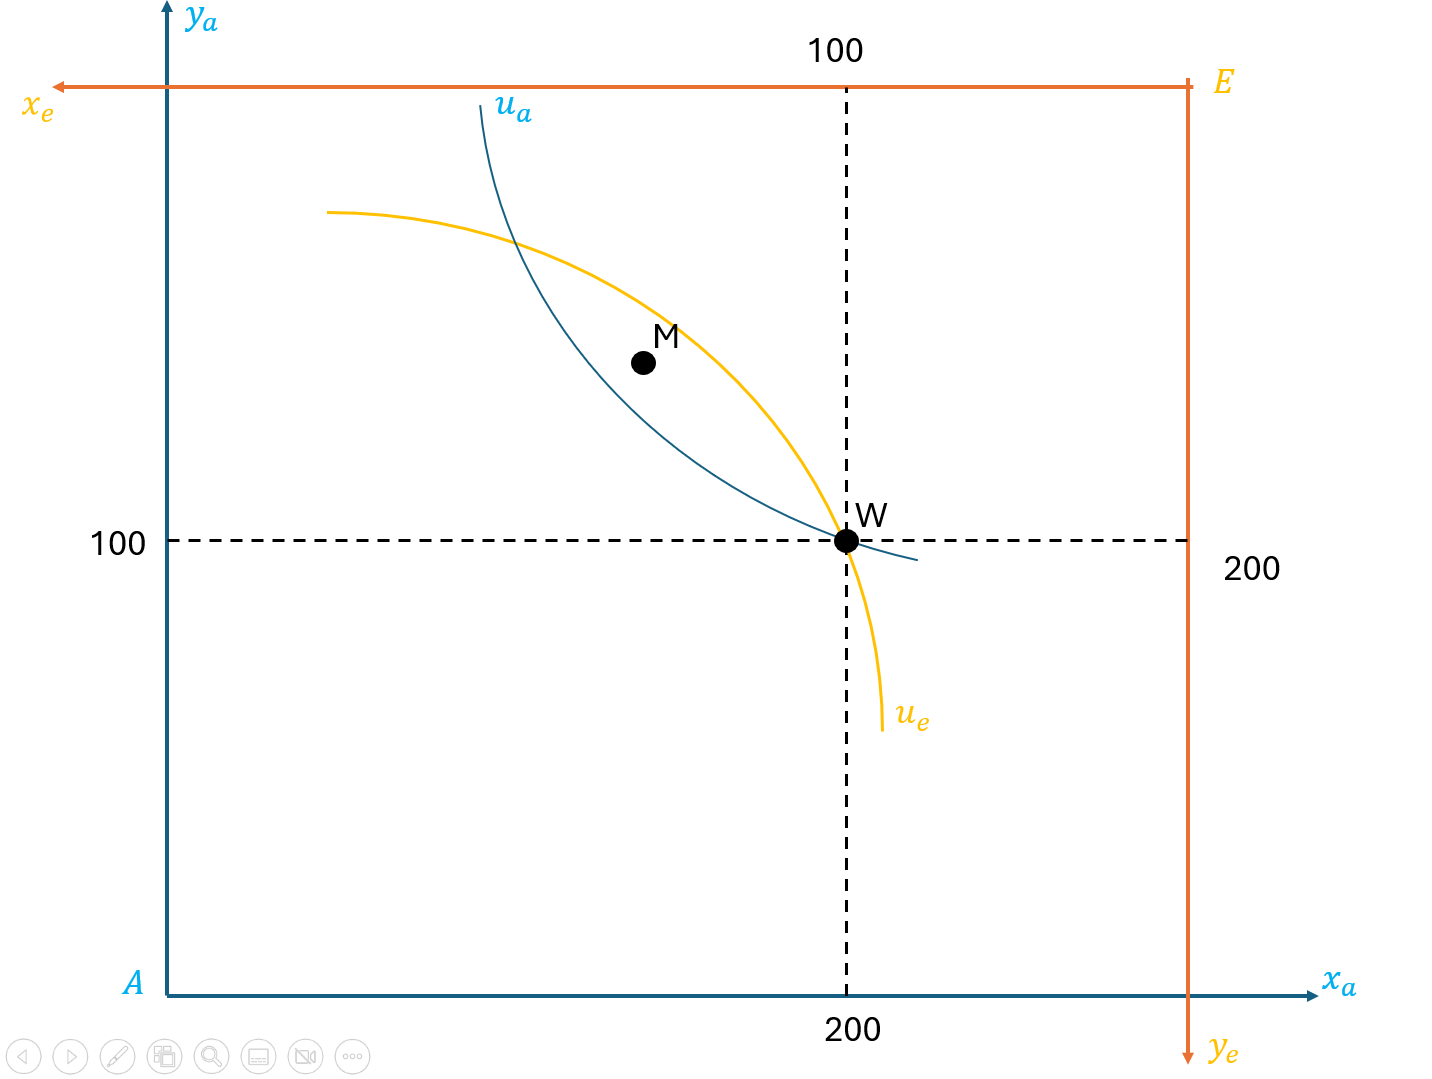
\includegraphics[width=0.70\linewidth]{Imagens/a2i11.png}
\end{figure}

\begin{figure}[H]
    \centering
    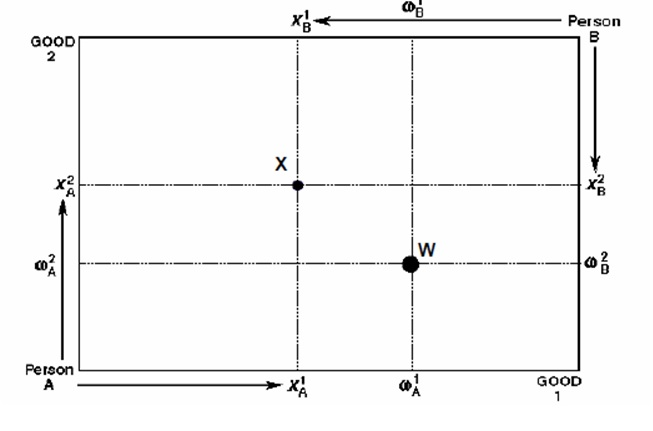
\includegraphics[width=0.70\linewidth]{Imagens/a2i1.png}
\end{figure}

Precisamos incluir as preferências dos consumidores

\begin{figure}[H]
    \centering
    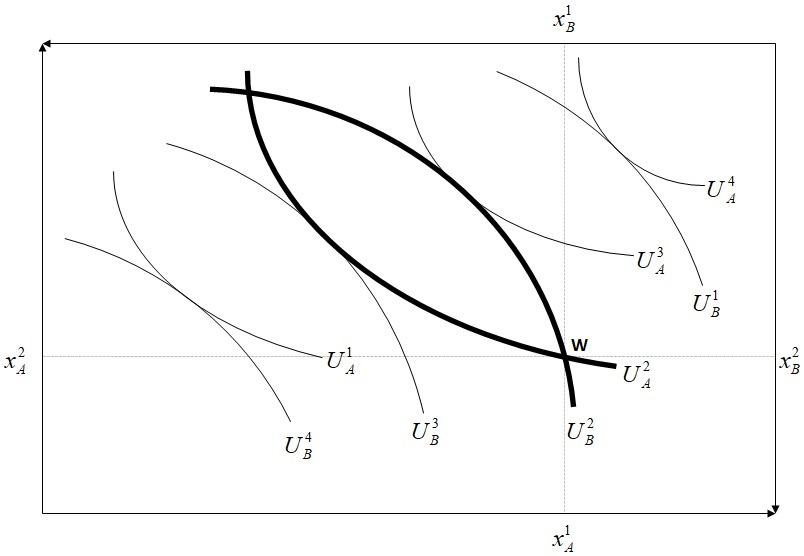
\includegraphics[width=0.70\linewidth]{Imagens/a2i2.png}
\end{figure}

Agora que temos a representação tanto das preferências quanto das dotações dos bens, podemos analisar como ocorrem as trocas

Partindo da dotação original (ponto W ), se ambos pudessem trocar seus bens, em qual região da caixa \textbf{os dois estariam em uma posição melhor?}

\begin{figure}[H]
    \centering
    
\includegraphics[width=0.70\linewidth]{Imagens/a2i3.png}
\end{figure}

Durante as negociações, os países chegarão a uma troca vantajosa que os moverá para um ponto dentro da área em formato de lente.

Não há nada particularmente especial sobre a alocação $M$. Qualquer alocação nessa região com forma de lente seria possível:
\begin{itemize}
    \item Há \textbf{ganhos de troca} nessa região.
\end{itemize}

De modo similar ao que fizemos anteriormente podemos:
\begin{itemize}
    \item Traçar as curvas de indiferença que passam por $M$.
    \item Construir uma nova região de vantagem mútua.
    \item Avaliar uma nova alocação em que os países aceitem a troca.
\end{itemize}

Poderíamos repetir esse processo até que nenhuma das partes tenha mais uma troca preferida. Quais as características de tal ponto?


\begin{figure}[H]
    \centering
    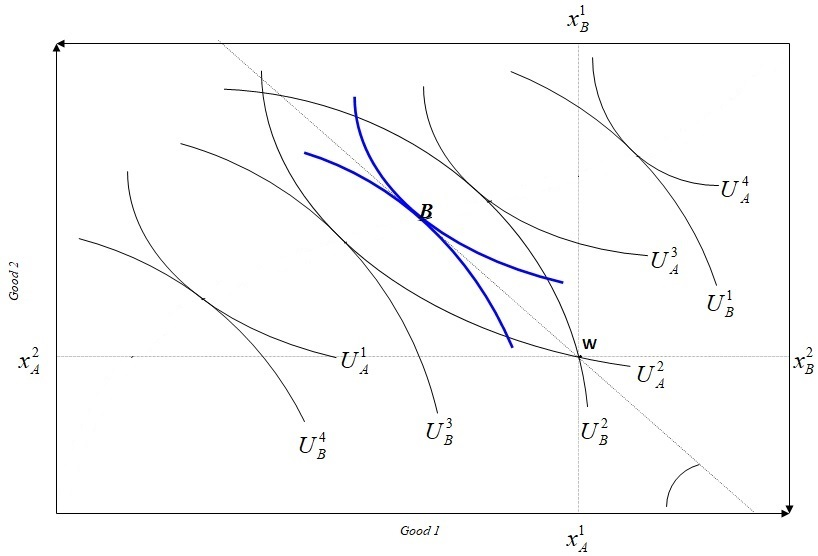
\includegraphics[width=0.70\linewidth]{Imagens/a2i4.png}
\end{figure}

Para que não existam mais trocas vantajosas para ambos os países, precisamos que as suas curvas de indiferença sejam tangentes

\textbf{Não} é possivel obter ganhos de troca no ponto B

Dizemos que B  é uma alocação \textbf{eficiente no sentido de Pareto}

O que significa esse conceito de \textbf{eficiência}?

\subsection{\textbf{Eficiência de Pareto}}

\textbf{Definição}

Em uma economia de trocas, uma alocação factível é \textbf{eficiente no sentido de Pareto} se não  for  possível  encontrar  uma  alocação  alternativa  em  que  pelo  menos  um  indivíduo esteja  melhor  e  nenhum  indivíduo  pior\begin{itemize}
    \item Vimos que se as curvas de indiferença dos consumidores se cruzarem, então terá de haver uma troca mutuamente vantajosa
    \item A partir da condição de tangência é fácil verificar que há muitas alocações eficientes no sentido de Pareto
\end{itemize}

Gostaríamos de ter um método para encontrar todas essas alocações eficientes

Dada uma curva de indiferença qualquer, mova-se ao longo dela até encontrar o melhor ponto para o outro consumidor

O conjunto de todas as alocações eficientes no sentido de Pareto é chamado de \textbf{curva de contrato} ou conjunto de Pareto

\begin{figure}[H]
    \centering
    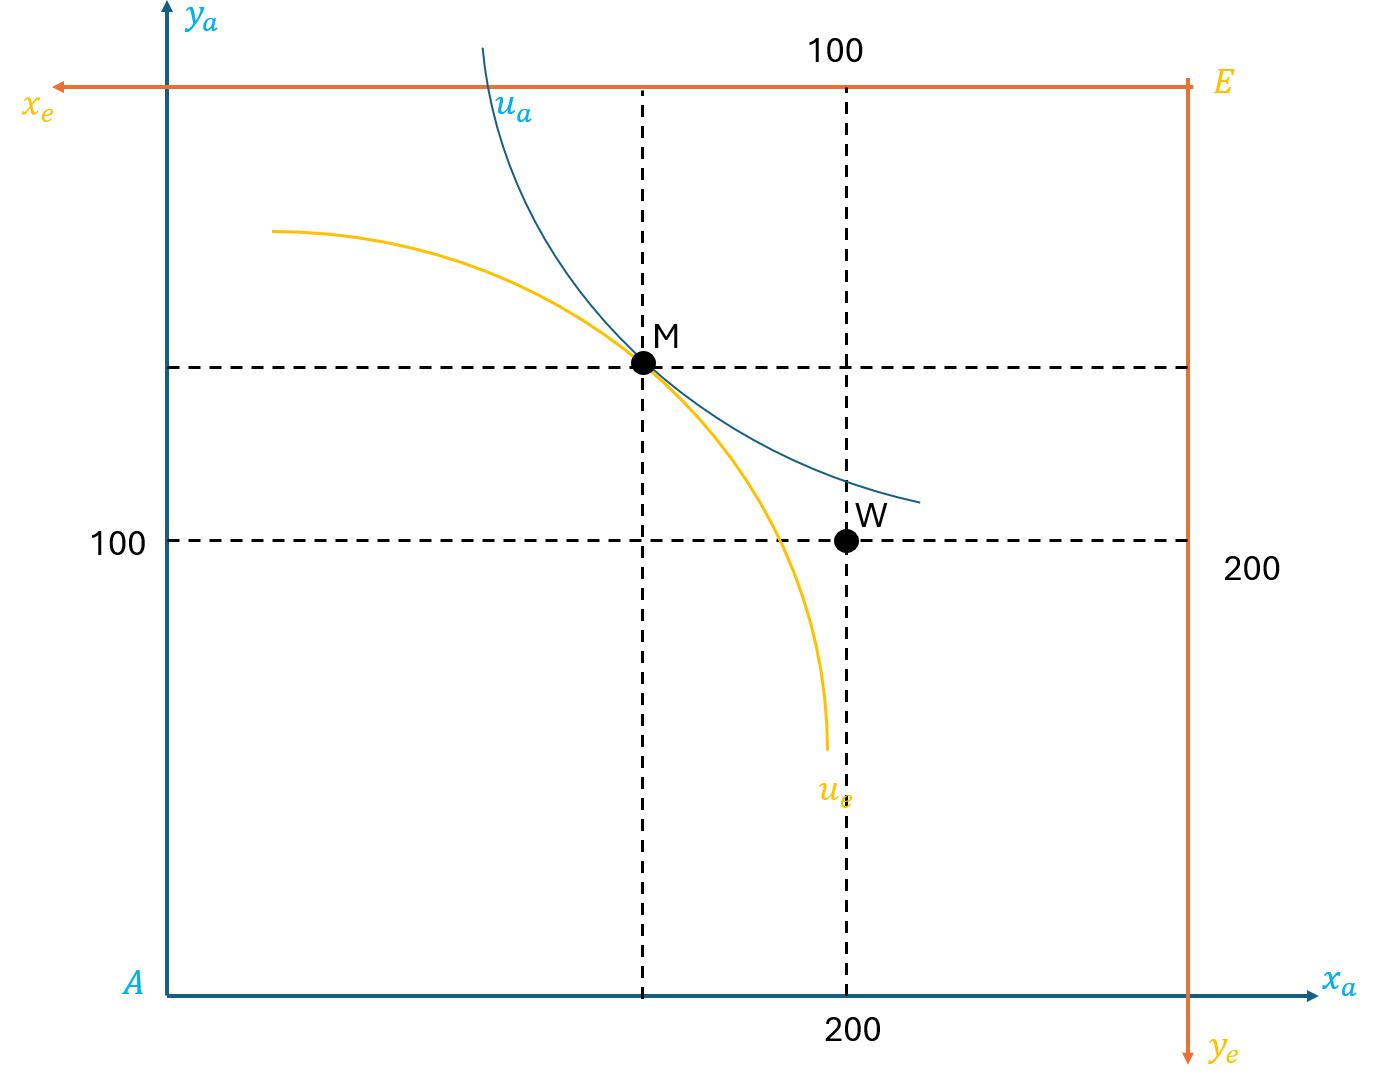
\includegraphics[width=0.70\linewidth]{Imagens/a2i12.png}
\end{figure}

\subsection{\textbf{Curva de Contrato}}

\begin{figure}[H]
    \centering
    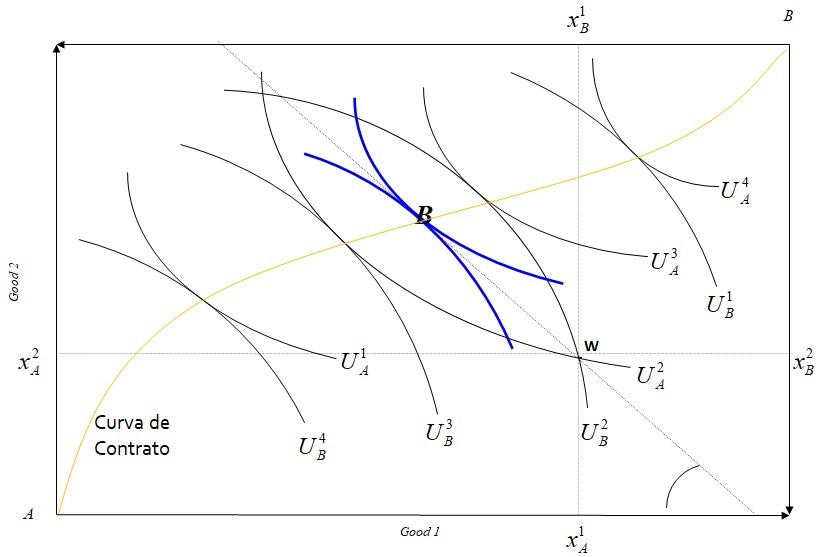
\includegraphics[width=0.70\linewidth]{Imagens/a2i5.png}
\end{figure}

\begin{figure}[H]
    \centering
    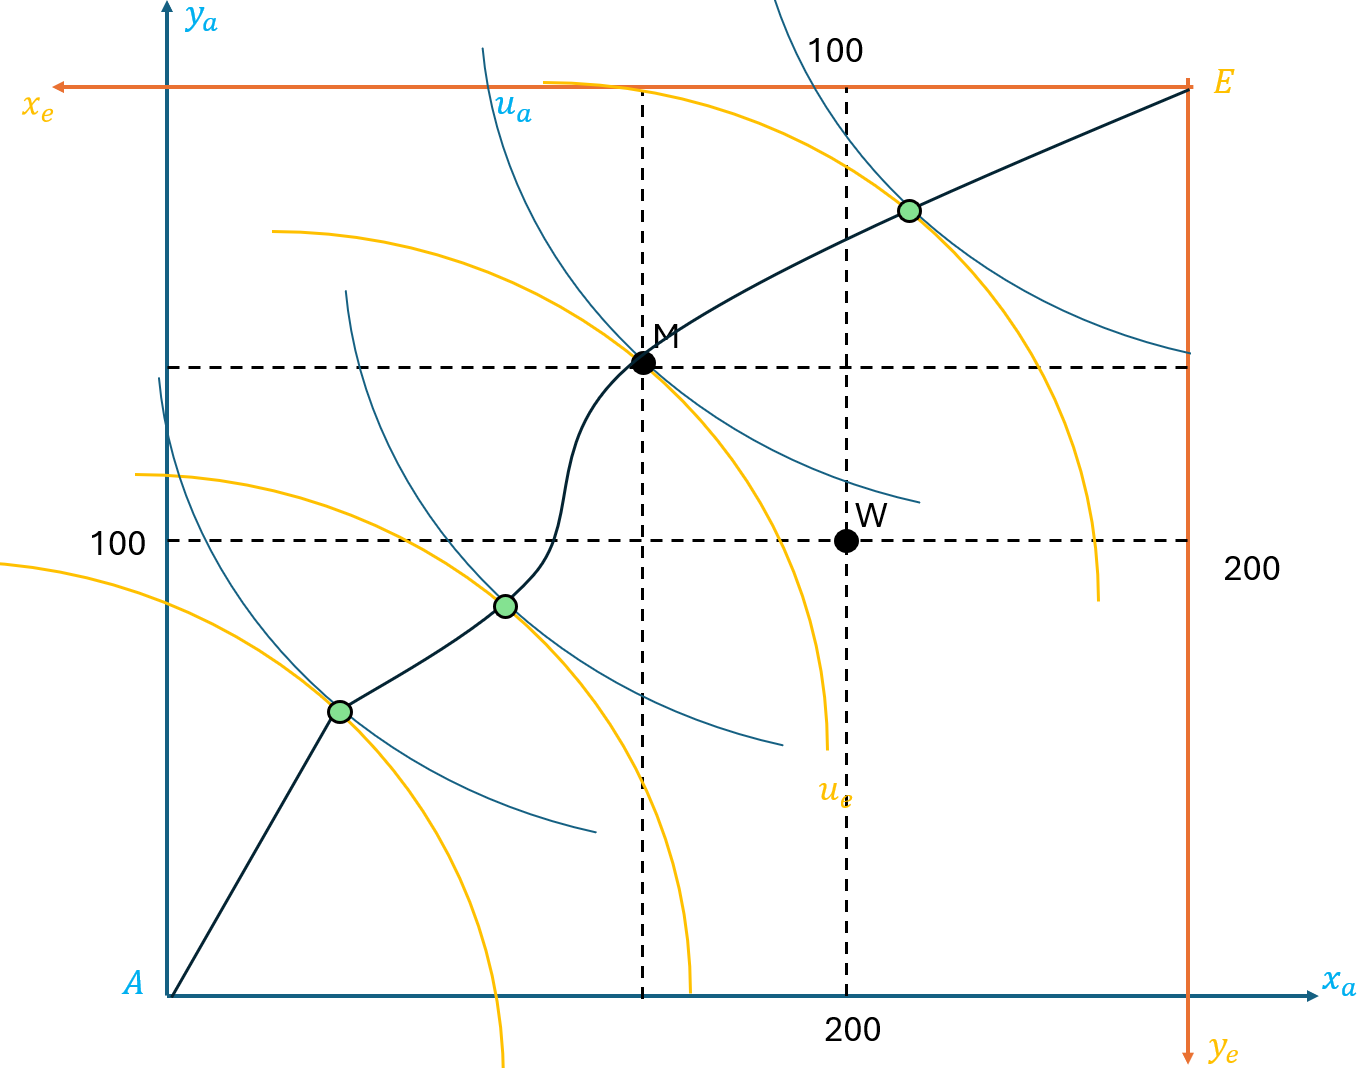
\includegraphics[width=0.70\linewidth]{Imagens/a2i13.png}
\end{figure}

\subsubsection{\textbf{Exercício de Curvas de Contrato}}

\textbf{Como calcular a Curva de Contrato?}

\begin{itemize}
    \item \textbf{Avançado:} \( u_A(x_A, y_A) = x_A^{3/4} y_A^{1/4} \)
    \item \textbf{Emergente:} \( u_E(x_E, y_E) = x_E^{1/4} y_E^{3/4} \)
    \item \textbf{Dotação:} \(w_A^x + w_E^x = 13 \quad ; \quad w_A^y + w_E^y = 10\)
\end{itemize}

\begin{itemize}
    \item Note que o conjunto de Pareto não depende de como a dotação inicial está distribuída entre os indivíduos.
    \item A dotação determina apenas as quantidades totais disponíveis de ambos os bens e, portanto, determina as dimensões da caixa.
\end{itemize}

Resolução\begin{enumerate}
    \item \textbf{Calcule as TMS de cada consumidor.}
    
    \begin{itemize}
        \item \emph{Consumidor A (Avançado):}  
        \[
            u_A(x_A, y_A) \;=\; x_A^{\frac{3}{4}}\,y_A^{\frac{1}{4}}.
        \]
        As derivadas parciais são:
        \[
            \frac{\partial u_A}{\partial x_A} 
            \;=\;\frac{3}{4}\,x_A^{-\frac{1}{4}}\,y_A^{\frac{1}{4}}, 
            \quad
            \frac{\partial u_A}{\partial y_A} 
            \;=\;\frac{1}{4}\,x_A^{\frac{3}{4}}\,y_A^{-\frac{3}{4}}.
        \]
        Assim, a TMS de A (razão entre as utilidades marginais) é
        \[
            \mathrm{TMS}_A 
            \;=\; 
            \frac{\frac{3}{4}\,x_A^{-\frac{1}{4}}\,y_A^{\frac{1}{4}}}
                 {\frac{1}{4}\,x_A^{\frac{3}{4}}\,y_A^{-\frac{3}{4}}}
            \;=\; 3\,\frac{y_A}{x_A}.
        \]

        \item \emph{Consumidor E (Emergente):}
        \[
            u_E(x_E, y_E) \;=\; x_E^{\frac{1}{4}}\,y_E^{\frac{3}{4}}.
        \]
        As derivadas parciais são:
        \[
            \frac{\partial u_E}{\partial x_E} 
            \;=\;\frac{1}{4}\,x_E^{-\frac{3}{4}}\,y_E^{\frac{3}{4}}, 
            \quad
            \frac{\partial u_E}{\partial y_E} 
            \;=\;\frac{3}{4}\,x_E^{\frac{1}{4}}\,y_E^{-\frac{1}{4}}.
        \]
        Logo, a TMS de E é
        \[
            \mathrm{TMS}_E 
            \;=\; 
            \frac{\frac{1}{4}\,x_E^{-\frac{3}{4}}\,y_E^{\frac{3}{4}}}
                 {\frac{3}{4}\,x_E^{\frac{1}{4}}\,y_E^{-\frac{1}{4}}}
            \;=\;\frac{1}{3}\,\frac{y_E}{x_E}.
        \]
    \end{itemize}
    
    \item \textbf{Imponha a condição de eficiência (igualar as TMS).}

    Num ótimo de Pareto,
    \[
        \mathrm{TMS}_A 
        \;=\; 
        \mathrm{TMS}_E 
        \;\;\Longrightarrow\;\;
        3\,\frac{y_A}{x_A} 
        \;=\; 
        \frac{1}{3}\,\frac{y_E}{x_E}.
    \]

    \item \textbf{Use as restrições de dotação total.}

    Sabemos que
    \[
        x_A + x_E = 13
        \quad\text{e}\quad
        y_A + y_E = 10.
    \]
    Logo,
    \[
        x_E = 13 - x_A
        \quad\text{e}\quad
        y_E = 10 - y_A.
    \]
    Substituindo na condição de eficiência:
    \[
        3\,\frac{y_A}{x_A}
        \;=\;
        \frac{1}{3}\,\frac{\,10 - y_A\,}{\,13 - x_A\,}.
    \]
    Multiplicando cruzado:
    \[
        9\,\frac{y_A}{x_A}
        \;=\;
        \frac{10 - y_A}{13 - x_A}
        \;\;\Longrightarrow\;\;
        9\,y_A\,(13 - x_A) \;=\; x_A\,(10 - y_A).
    \]

    \item \textbf{Expressar a Curva de Contrato.}

    A equação
    \[
        9\,y_A\,(13 - x_A) 
        \;=\; 
        x_A\,(10 - y_A)
    \]
    relaciona \((x_A,y_A)\) dentro da caixa de Edgeworth e define a Curva de Contrato. Para isolá-la, podemos escrever:
    \[
        9\,y_A\,(13 - x_A) 
        \;=\; 
        x_A\,(10 - y_A)
        \;\;\Longrightarrow\;\;
        117\,y_A - 9\,x_A\,y_A 
        \;=\; 
        10\,x_A - x_A\,y_A,
    \]
    \[
        117\,y_A 
        \;=\; 
        10\,x_A + 8\,x_A\,y_A
        \;\;\Longrightarrow\;\;
        117\,y_A - 8\,x_A\,y_A 
        \;=\; 
        10\,x_A,
    \]
    \[
        y_A\,\bigl(117 - 8\,x_A\bigr)
        \;=\;
        10\,x_A
        \;\;\Longrightarrow\;\;
        y_A
        \;=\;
        \frac{10\,x_A}{117 - 8\,x_A}.
    \]
    Esta é a equação da Curva de Contrato, sujeita às restrições de não‐negatividade e à disponibilidade total dos bens.
    \item \begin{figure}[H]
    \centering
    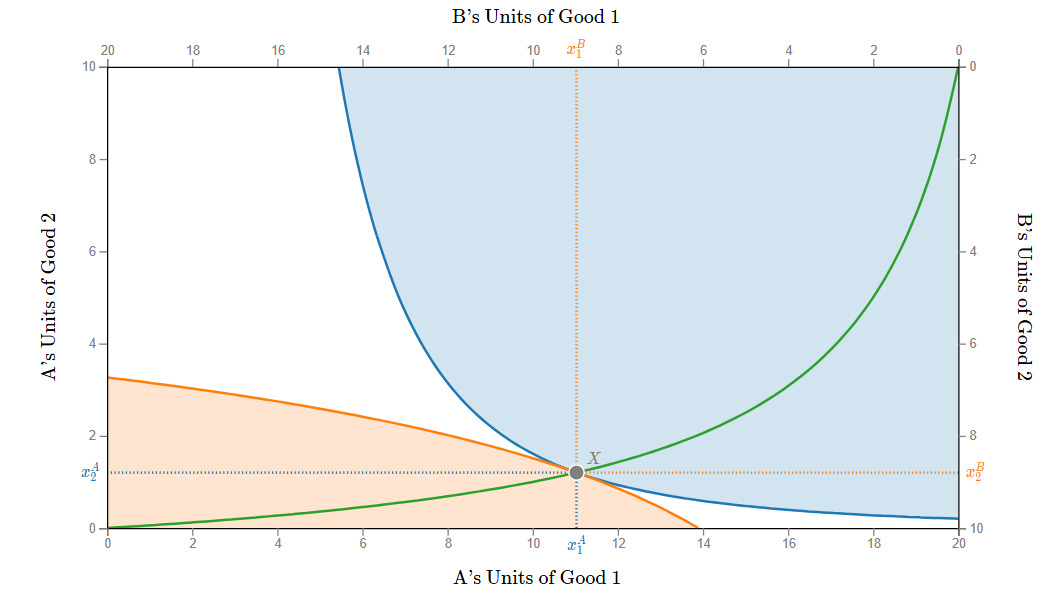
\includegraphics[width=0.70\linewidth]{Imagens/a2i14.png}
\end{figure}
\end{enumerate}


\subsection{\textbf{Equilíbrio Competitivo}}

Vimos uma ferramente muito útil para determinar as possíveis trocas entre as economias, que no caso seria a caixa de Edgeworth. Mas há pontos que pontos sobre a curva de contrato que podem ser atingidos via poder de barganha, em que um país vai "tirar" vantagem do outro para aumentar sua utilidade em detrimento do outro. Lembrando que não falamos de preços ainda, somente quantidades e essas quantidades eram pré-determinadas e limitadas.

Com preço, saberemos onde na curva de estaremos. 

\textbf{Como descrever o equilíbrio de maneira mais precisa?}\begin{itemize}
   \item  Discutimos como o conceito de eficiência no sentido de Pareto está associado com a inexistência de uma troca mutuamente benéfica
   \item  O grande problema com o processo de trocas descrito é que ele é muito impreciso
   \item  Aprendemos que a alocação final estará localizada sobre a curva de contrato, mas não conseguimos prever exatamente qual será essa alocação
   \item  Para tentar resolver esse problema, vamos tentar um processo diferente
\end{itemize}

Imagine a figura de um “leiloeiro”, o qual escolhe um vetor de preços ($p_x,p_y$)  para os bens e o apresenta aos agentes da nossa economia. Isso acaba por garantir que a oferta seja igual a demanda, garantindo a alocação factível. Para isso, iremos usar da ideia de restrição orçamentária: $P_xx_A+P_yy_A=I=P_xw_A^x+P_yw_A^y$.
\[
y_A=\frac{I}{P_y}-\underbrace{\frac{P_x}{P_y}}_{\text{Inclinação}}x_A
\]
\href{https://www.econgraphs.org/graphs/exchange/edgeworth_box/trading_at_price_ratio}{Gráfico Interativo de Caixa de Edgeworth com Restrição Orçamentária}

\begin{figure}[H]
    \centering
    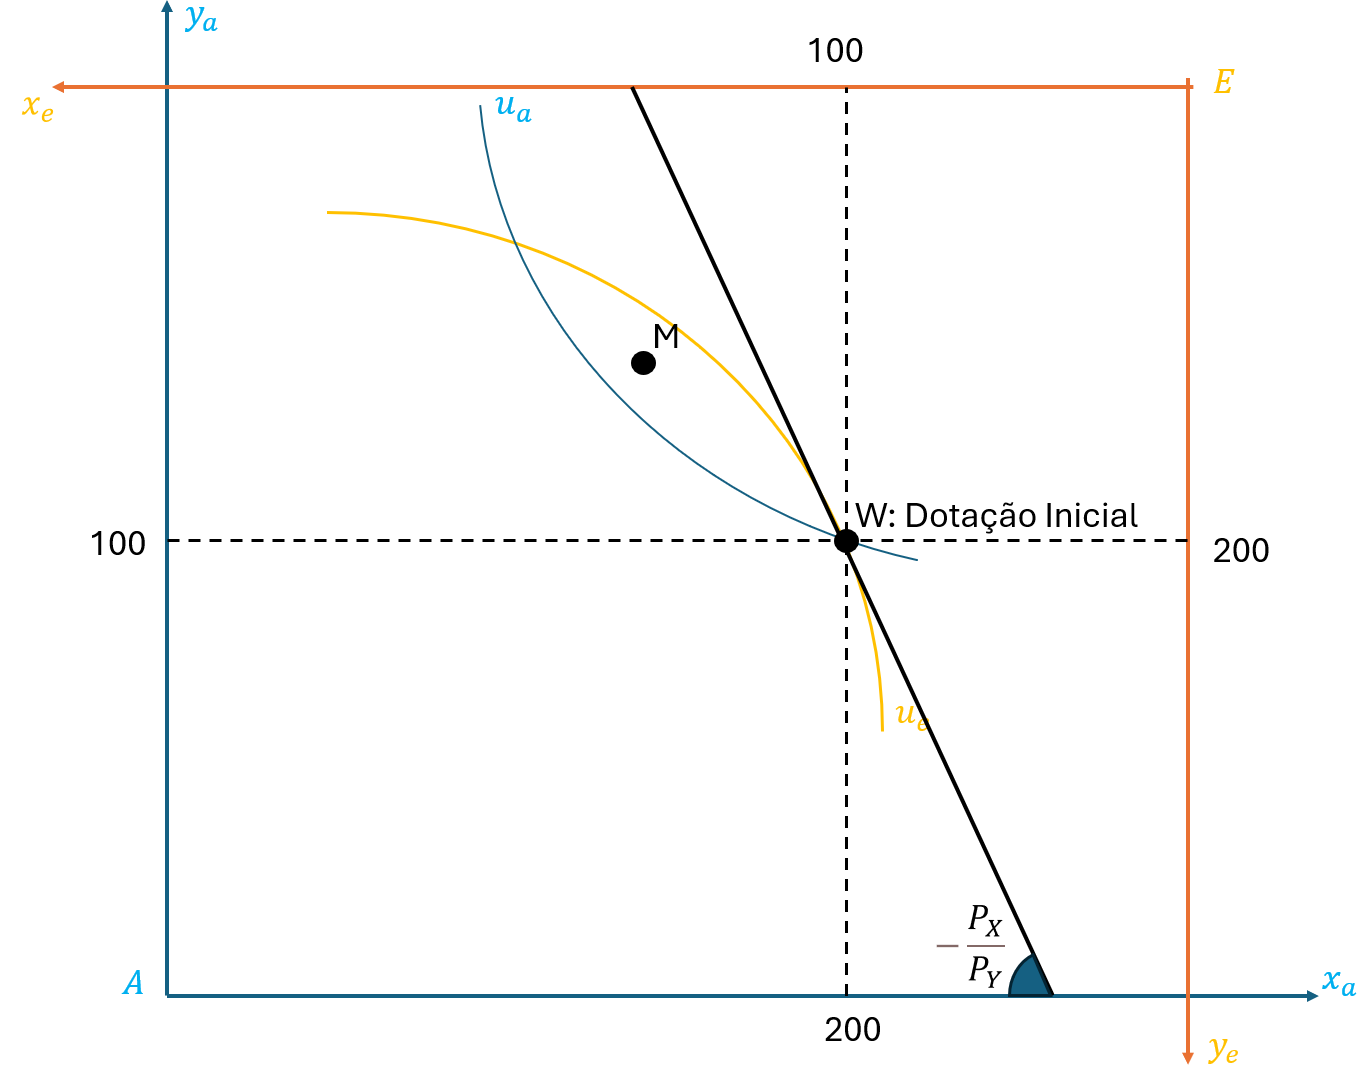
\includegraphics[width=0.70\linewidth]{Imagens/a3i8.png}
\end{figure}

Cada agente calcula, então, quanto vale a sua dotação e decide quanto de cada bem deseja comprar a esses preços.

Graficamente, a solução do problema do consumidor é caracterizada pelo ponto em que a sua curva de indiferença é tangente à restrição orçamentária.

Se representarmos tal ponto para os nossos dois países na caixa de Edgeworth, teremos a seguinte configuração

\begin{figure}[H]
    \centering
    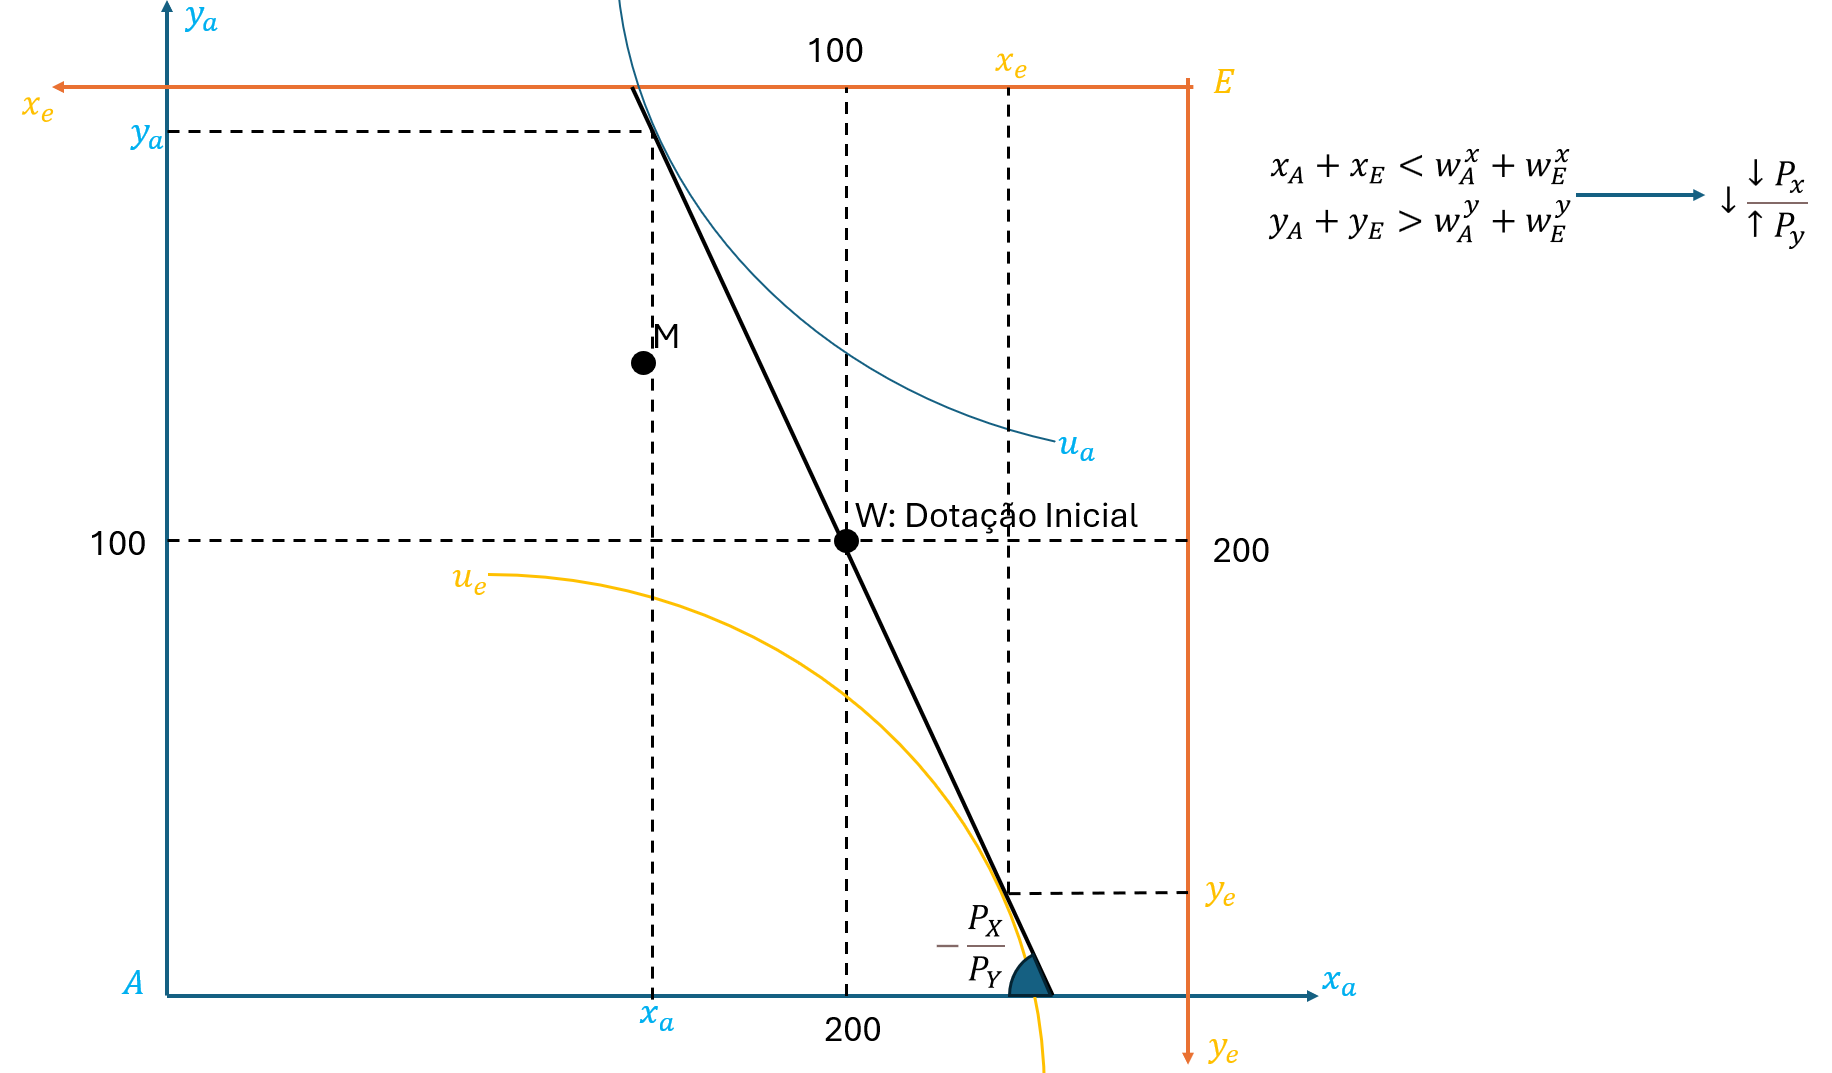
\includegraphics[width=0.70\linewidth]{Imagens/a3i9.png}
\end{figure}

\begin{figure}[H]
    \centering
    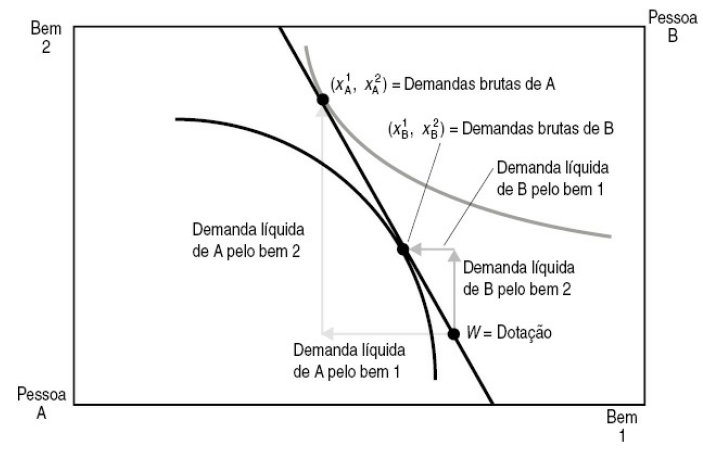
\includegraphics[width=0.70\linewidth]{Imagens/a2i6.png}
\end{figure}



Note que nada garante que a oferta se iguale à demanda para os preços arbitrários $(p_x, p_y)$. De fato, percebemos que
\[
x_A + x_E < w_A^x + w_E^x
\]
\[
y_A + y_E > w_A^y + w_E^y
\]

Ou seja, existe um excesso de oferta pelo bem $x$ (manufaturado) e um excesso de demanda pelo bem $y$ (agrícola).

Quando tal situação acontece, dizemos que o vetor de preços $(p_x, p_y)$ \textbf{não} equilibra os mercados para os dois bens.

Nessa situação, o leiloeiro \textbf{mudará os preços dos bens}

Se houver excesso de demanda por um dos bens, o leiloeiro aumentará o preço desse bem

Se houver excesso de oferta de um dos bens, o leiloeiro reduzirá o preço desse bem

Esse processo de ajustamento continua até que a demanda de cada um dos bens se iguale à oferta. Como será a configuração final?

\begin{figure}[H]
    \centering
    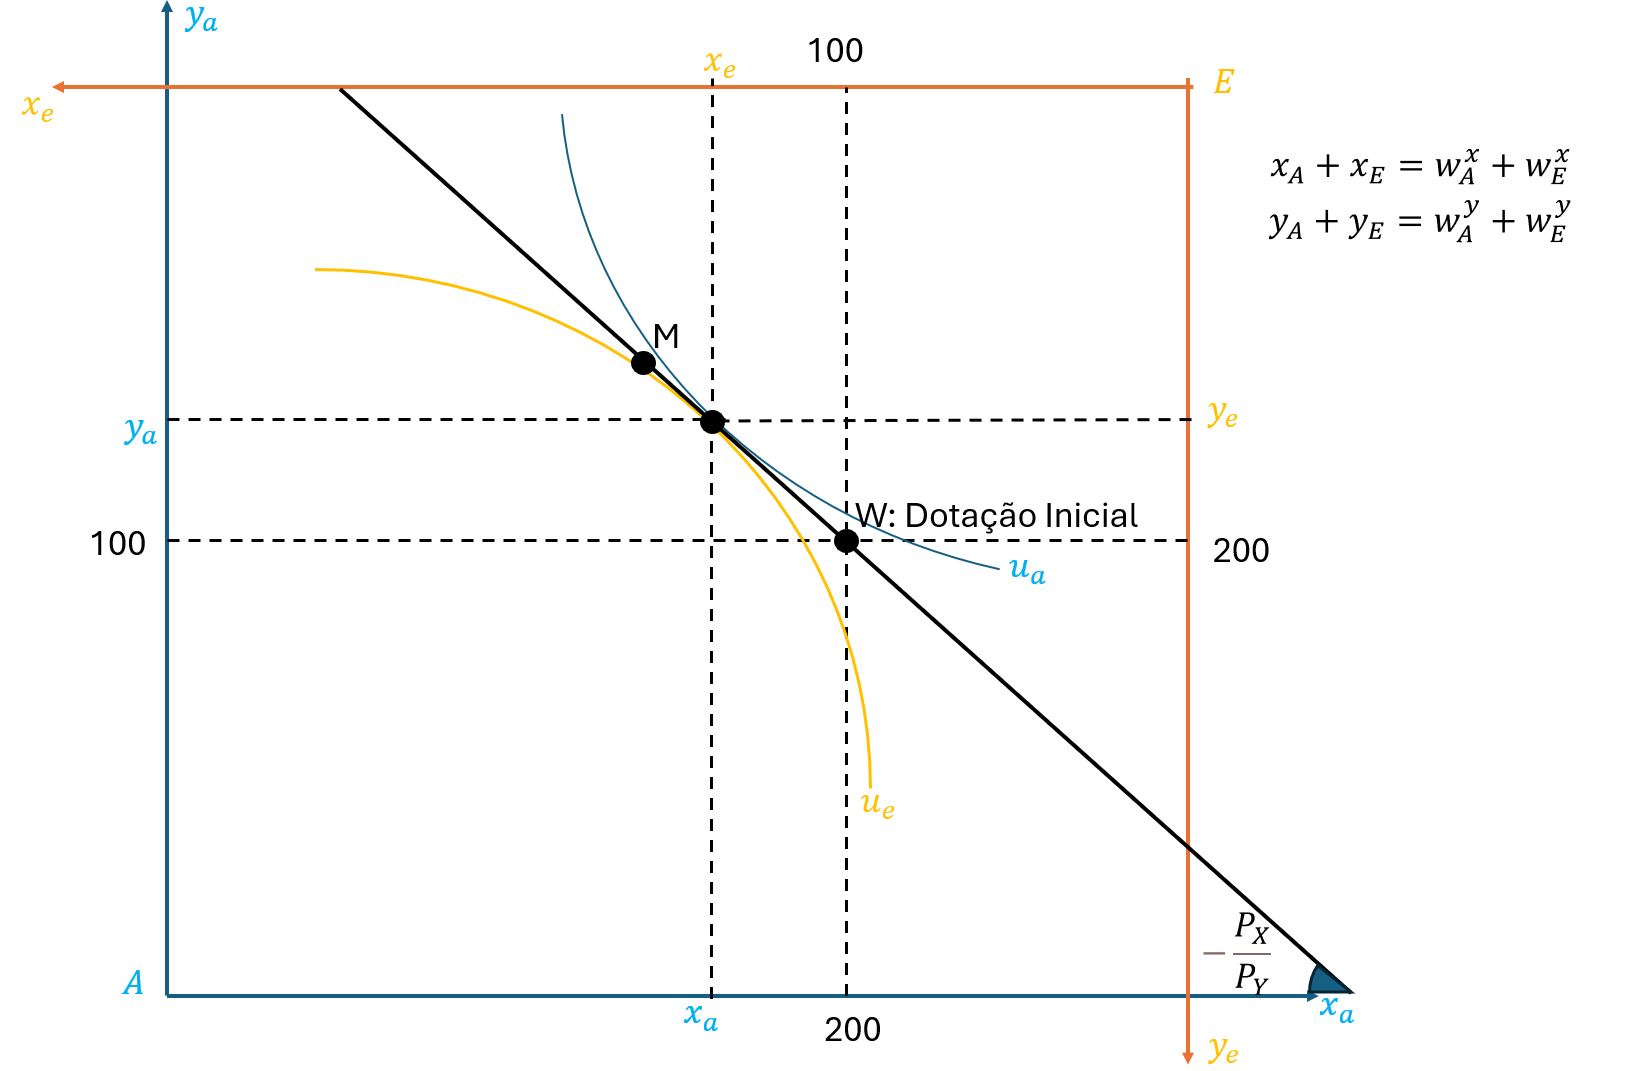
\includegraphics[width=0.70\linewidth]{Imagens/a3i10.png}
\end{figure}

Lembrando que essa solução(e todas as solução válidas) está sobre a cruva de contrato.


\begin{figure}[H]
    \centering
    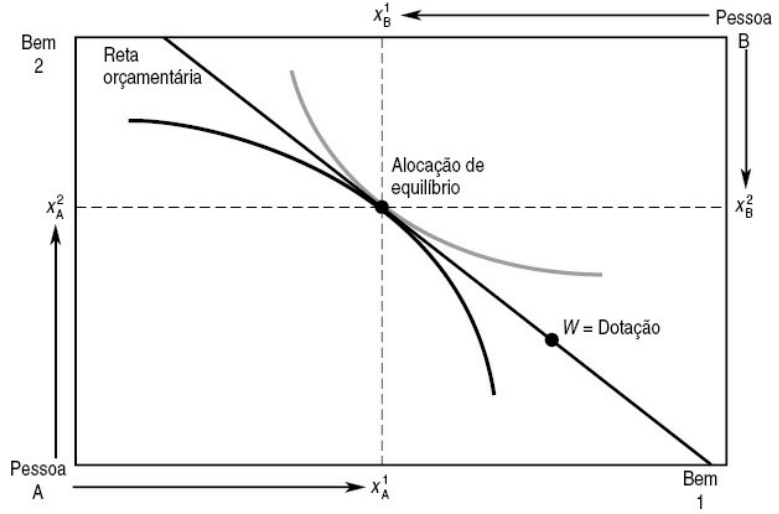
\includegraphics[width=0.70\linewidth]{Imagens/a2i7.png}
\end{figure}

Agora, a quantidade total que cada agente deseja comprar de cada bem, aos preços correntes, é igual à quantidade total disponível

Dizemos, portanto, que o mercado está em equilíbrio

\textbf{Definição}: Um equilíbrio competitivo constitui-se de uma alocação e um vetor de preços que satisfazem duas condições\begin{enumerate}
    \item Dado o vetor de preços, a cesta de escolha referente ao agente i  é uma solução para o seu problema do consumidor
    \item A alocação deve ser factível, ou seja, a demanda deve ser igual à oferta em todos os mercados
\end{enumerate}

\subsection{\textbf{Lei de Walras}}

Como podemos ter certeza de que todos os mercados estão equilibrados? Lembrando :
\[
P_xx_A+P_yy_A=P_xw_A^x+P_y^Y
\]

\[
P_x(x_A-w_A^x)+P_y(y_A-w_A^y) = 0 \ (1)
\]
\[
P_x(x_E-w_E^x)+P_y(y_E-w_E^y) = 0 \ (2)
\]

(1)+(2) = $P_x\underbrace{(x_A-w_A^x+x_E-w_E^x)}_{z_x}+P_y\underbrace{(y_A-w_A^y+y_E-w_E^y)}_{z_y}=0\rightarrow P_xz_x+P_yz_y=0$

As funções \textbf{excesso de demanda agregada} são
\[
z_x(p_x, p_y) = x_A(p_x, p_y) - w_A^x + x_E(p_x, p_y) - w_E^x
\]
\[
z_y(p_x, p_y) = y_A(p_x, p_y) - w_A^y + y_E(p_x, p_y) - w_E^y
\]

A \textbf{Lei de Walras} afirma que
\[
p_x z_x(p_x, p_y) + p_y z_y(p_x, p_y) = 0,
\]
ou seja, o valor do excesso de demanda agregada é sempre igual a zero (para todas as escolhas de preços possíveis).


\subsection{\textbf{Equilíbrio e Eficiência}}

Note que, se cada agente escolher a melhor cesta que puder pagar, a TMS entre dois bens tem de ser igual à razão dos preços

Mas se todos os consumidores se defrontam com os mesmos preços, então, no equilíbrio, todos devem ter a \textbf{mesma} TMS

Isso significa que as curvas de indiferença dos dois agentes devem ser tangentes

Portanto, segue que \textbf{o equilíbrio competitivo é eficiente no sentido de Pareto!}

\subsubsection{\textbf{Primeiro Teorema do Bem-Estar}}

Todo equilíbrio competitivo é uma alocação eficiente no sentido de Pareto

Premissas\begin{itemize}
    \item Não há externalidade no consumo
    \item Agentes se comportam de maneira competitiva
\end{itemize}

Tal alocação pode não ter outras propriedades desejáveis, mas será necessariamente eficiente

Se você fosse economista-chefe do Banco Mundial, como compararia os pontos B,C e Q*? O ponto que \(Q^*\) apesar dela ser um ponto eficiente, dado que está sobre a curva de contrato e tangenciando a curva de restrição orçamentário, ela é muito desigual, dado que a dotação do país A é maior que a de E, seria interessante redistribuir as quantidades entre os países, isso pode ser feito através de uma transferência de renda. Assim desloca as utilidades, criando uma nova região de lente, que fica mais no "centro" do gráfico que seria mais igual. Depois deixariámos o mercado agir por sí só.   

\begin{figure}[H]
    \centering
    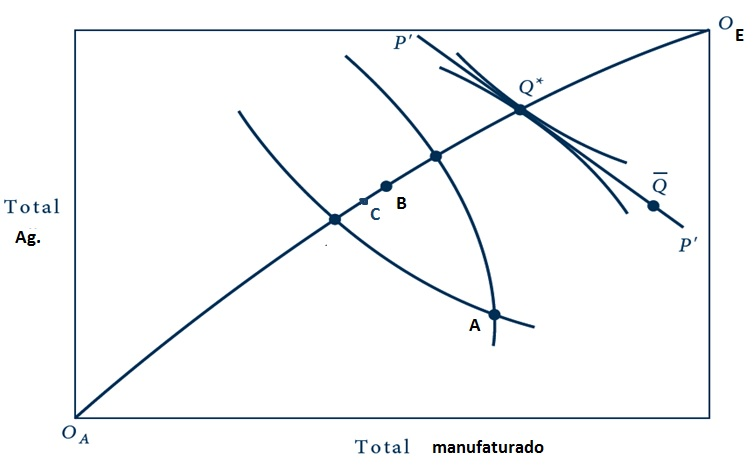
\includegraphics[width=0.70\linewidth]{Imagens/a2i8.png}
\end{figure}

O Primeiro Teorema do Bem-Estar não diz nada sobre a distribuição dos benefícios econômicos\begin{itemize}
    \item Equilíbrio competitivo depende da dotação inicial
\end{itemize}

Suponha que a dotação inicial da economia seja muito desigual\begin{itemize}
    \item O equilíbrio competitivo baseado nesta alocação inicial também seria injusto
\end{itemize}

Suponha ainda que a sociedade tenha decidido que há uma alocação eficiente no sentido de Pareto mais justa e desejável

Podemos encontrar preços que façam essa alocação constituir um equilíbrio de mercado?

Seja X   uma alocação Pareto-eficiente. Como sabemos, as curvas de indiferença dos dois agentes devem ser tangentes neste ponto

Suponha que associemos à economia acima um vetor de preços que induza como reta orçamentária exatamente a reta que separa as curvas de indiferença dos dois agentes

Escolha uma dotação inicial sobre esta reta orçamentária

Se cada agente escolher a melhor cesta em seu conjunto orçamentário, o equilíbrio resultante será a alocação Pareto-eficiente

\begin{figure}[H]
    \centering
    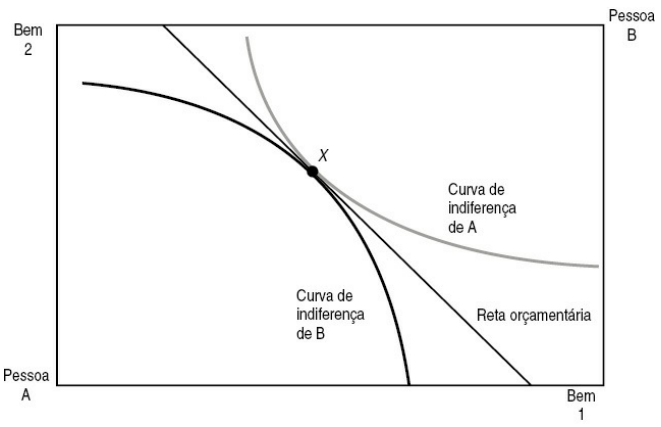
\includegraphics[width=0.70\linewidth]{Imagens/a2i9.png}
\end{figure}

Sempre podemos escolher uma dotação inicial e um vetor de preços de modo a fazer uma dada alocação eficiente parte de um equilíbrio competitivo?

Infelizmente nem sempre conseguimos alcançar alocações eficientes por mercados competitivos

\subsubsection{\textbf{Segundo Teorema do Bem-Estar}}

Se todos os agentes tiverem preferências estritamente convexas haverá sempre um conjunto de preços tal que cada alocação eficiente no sentido de Pareto seja um equilíbrio competitivo para uma distribuição apropriada de dotações
O Segundo Teorema de Bem-Estar implica que os problemas de distribuição e eficiência podem ser separados\begin{itemize}
    \item Papel alocativo dos preços: indicar a escassez relativa
    \item Papel distributivo dos preços: determinar quanto os agentes podem comprar
\end{itemize}

\subsection{\textbf{Equilíbrio Competitivo Exercício}}

\textbf{País Emergente:} $W_E = (w_E^x, w_E^y) = (100, 200)$ 

\textbf{País Avançado:} $W_A = (w_A^x, w_A^y) = (200, 100)$ 

\textbf{Preferências:} $u_i(x_i, y_i) = x_i^{1/2} y_i^{1/2}, \, i \in \{A, E\}$

\begin{enumerate}
    \item Encontre o equilíbrio competitivo (preços e quantidades) de autarquia(situação que não tem comércio; economia fechada) e de livre comércio.\begin{enumerate}
        \item Vamos montar o problema de maximização da utilidade de um País(no caso país A)
        \[
        \max_{x_A,y_A}u_A=x_A^{1/2}y_A^{1/2} \ \ s.a \ \ P_xx_A+P_yy_A=I=P_xw_A^x+P_yw_A^y
        \]
        \[
        \mathcal{L}=x_A^{1/2}y_A^{1/2} +\lambda(I-P_xx_A-P_yy_A)
        \]
        CPO's
        \[
        [x_A]:\frac{1}{2}x_A^{-1/2}y_A^{1/2}-\lambda P_x=0
        \]
        \[
        [y_A]:\frac{1}{2}x_A^{1/2}y_A^{-1/2}-\lambda P_y=0
        \]
        \[
        [\lambda]:I-P_xx_A-P_yy_A=0
        \]
        \[
        \frac{[x_A]}{[y_A]}=TMS=\frac{y_A}{x_A}=\frac{P_x}{P_y}
        \]
        \[
        y_A=\frac{P_xx_A}{P_y}
        \]
        \[
        I-P_xx_A-P_y\frac{P_xx_A}{P_y}=0 
        \]
        \[
        x_a=\frac{I}{2P_x} = \frac{P_xw_A^x+P_yw_A^y}{2P_x}=\frac{200P_x+100P_y}{2P_x}=100+\frac{50P_y}{P_x}
        \]
        \[
        y_A=\frac{I}{2P_y}=\frac{P_xw_A^x+P_yw_A^y}{2P_y}=\frac{200P_y+100P_x}{2P_y}=\frac{100P_x}{P_y}+50
        \]
    \item Vamos montar o problema de maximização da utilidade de um País(no caso país E; que é espelhada do País A)
        \[
        \max_{x_E,y_E}u_E=x_E^{1/2}y_E^{1/2} \ \ s.a \ \ P_xx_E+P_yy_E=I=P_xw_E^x+P_yw_E^y
        \]
        \[
        x_E=\frac{I}{2P_x}=\frac{100P_x+200P_y}{2P_x}=50+\frac{100P_y}{Px}
        \]
        \[
        y_E=\frac{I}{2P_y}=\frac{100P_x+200P_y}{2P_y}=\frac{50P_x}{P_y}+100
        \]
    \item Equilíbrio (Autarquia)\begin{itemize}
        \item Para o país avançado, eu preciso de \(x_A=w_A^x\rightarrow \underbrace{100+\frac{50P_y}{P_x}}_{x_A}=\underbrace{200}_{w_A^x}\rightarrow \frac{P_x}{P_y}=\frac{1}{2}\) e \(y_A=w_A^y\), dado a Lei de Walvas, como um dos mercados está em equilíbrio, o outro vai necessariamente vai estar, logo não preciso fazer o \(y_A=w_A^y\)
        \item \item Para o país emergente, eu preciso de \(x_E=w_E^x\rightarrow \underbrace{50+\frac{100P_y}{P_x}}_{x_E}=\underbrace{200}_{w_E^x}\rightarrow \frac{P_x}{P_y}=2\) e \(y_E=w_E^y\), dado a Lei de Walvas, como um dos mercados está em equilíbrio, o outro vai necessariamente vai estar, logo não preciso fazer o \(y_E=w_E^y\)
    \end{itemize}
    \item Equilíbrio (Comércio)\begin{itemize}
        \item Eu preciso garantir que \(x_A+x_E=w_A^x+w_E^x\) e \(y_A+y_E=w_A^y+w_E^y\), vamos usar a Lei de Walras, por uma questão de praticidade, \(\underbrace{100+\frac{50P_y}{P_x}}_{x_A}+\underbrace{50+\frac{100P_y}{Px}}_{x_E}=300\rightarrow\frac{Px}{Py}=1\)
        \item \(x_A=150\) , \(y_A=150\), \(x_E=150\) e \(y_E=150\) 
    \end{itemize}
    
    \end{enumerate}
    \item Represente em um único gráfico os equilíbrios competitivos de autarquia e de livre comércio (um gráfico para cada país).\begin{enumerate}
        \item Olhando para o país emergente sobre uma autarquia e livre comércio.\begin{itemize}
            \item \(P_xx_E+P_yy_E=P_xw_E^x+P_yw_E^y= P_x100+P_y200\)
            \item \(y_E= \frac{P_x100+P_y200}{Py}-\frac{Px}{Py}x_E\)
            \item \(y_E=200+200-2x_E=400-2x_E\) \textbf{Autarquia}
            \item \(y_E=100+200-2x_E=300-1x_E\) \textbf{Comércio}
            \begin{figure}[H]
            \centering
            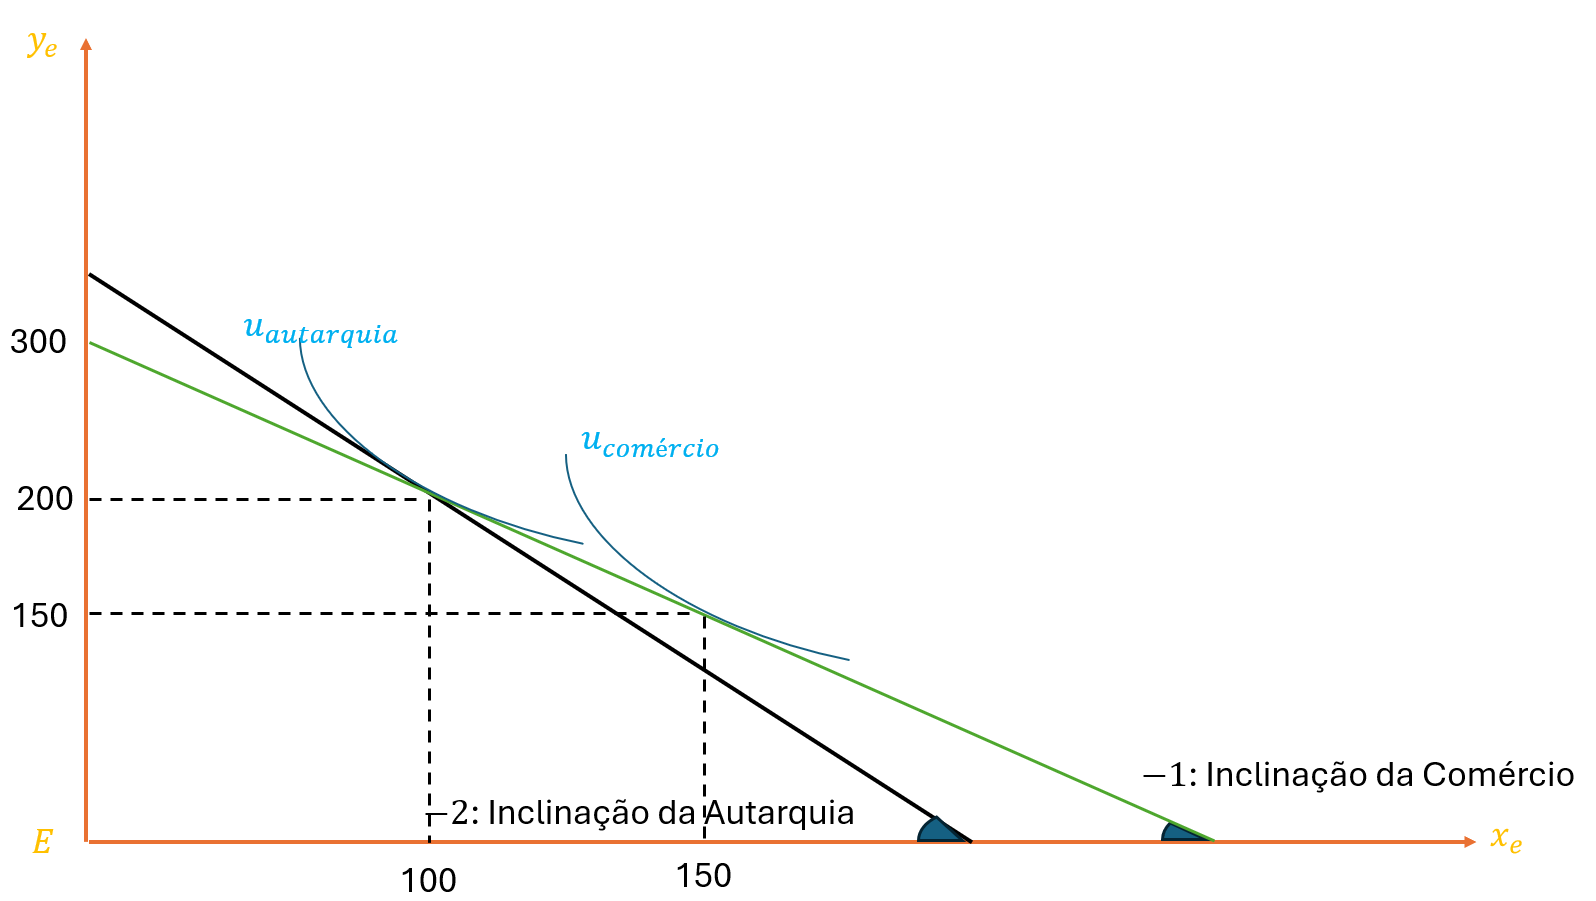
\includegraphics[width=0.7\linewidth]{Imagens/a4i1.png}
            \end{figure}
        \end{itemize}
        \item Olhando para o país avançado sobre uma autarquia e livre comércio.\begin{itemize}
            \item \(P_xx_A+P_Ay_A=P_xw_E^xP_yw_E^y=P_x200+P_y100\)
            \item \(y_A=\frac{P_x200+P_y100}{Py}-\frac{Px}{Py}x_A\)
            \item \(y_A= 100+100 - \frac{1}{2}x_A=200-\frac{1}{2}x_A\)\textbf{Autarquia}
            \item \(y_A= 200 + 100 -1x_A=300-1x_A\)\textbf{Comércio}
            \begin{figure}[H]
                \centering
                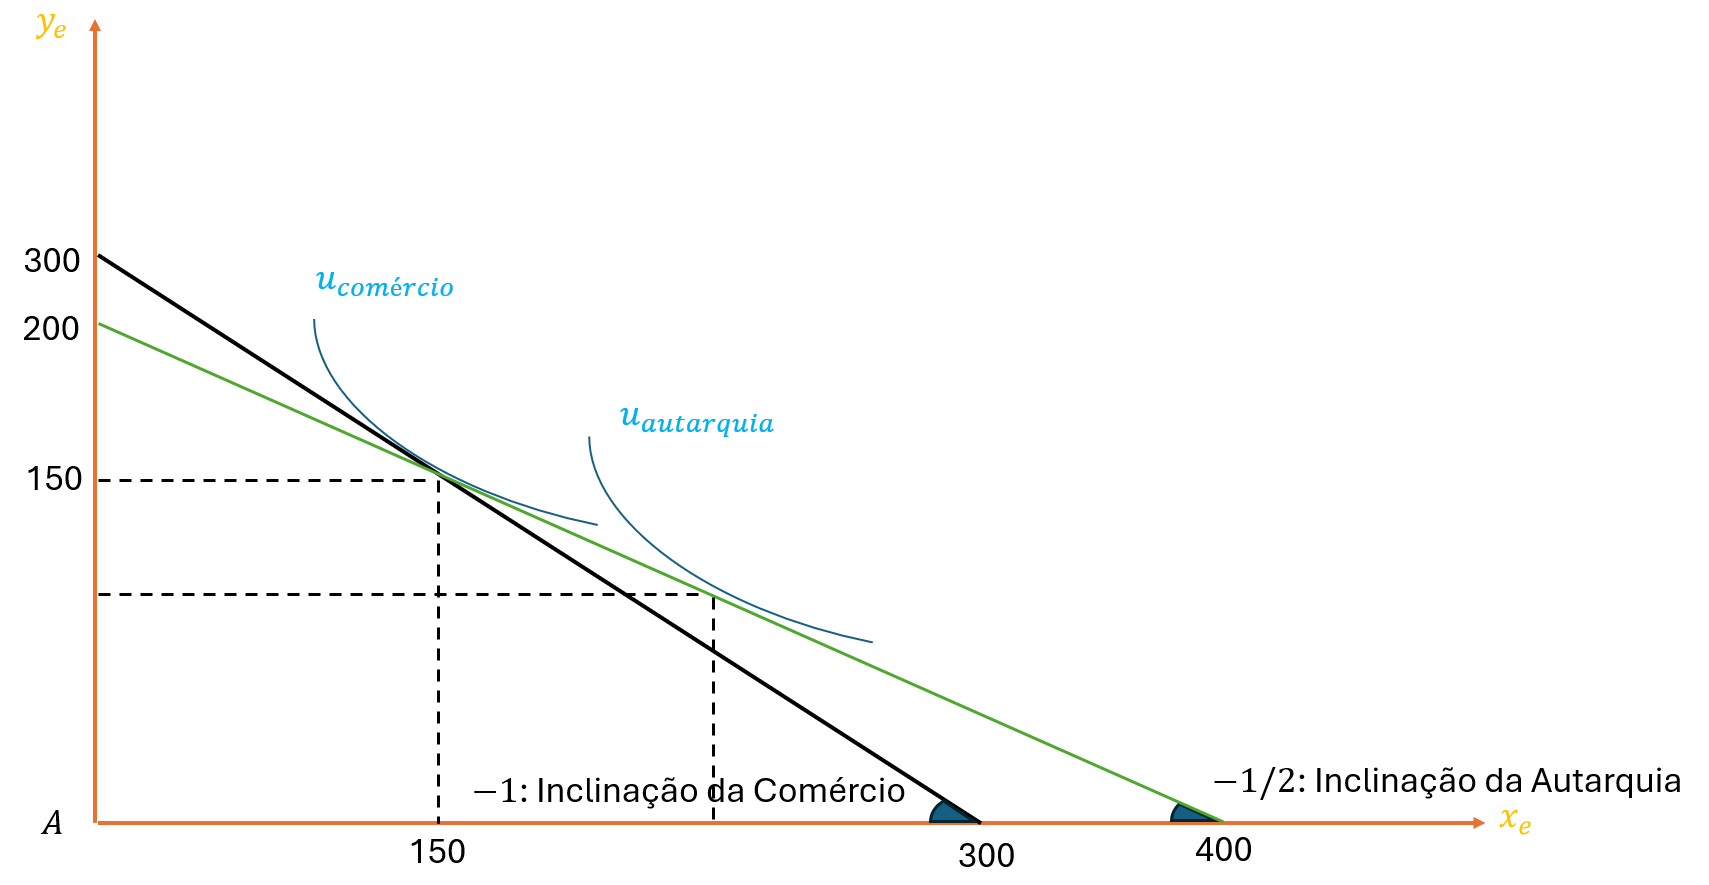
\includegraphics[width=0.7\linewidth]{Imagens/a4i2.png}
            \end{figure}
        \end{itemize}
        \end{enumerate}
    
    \item Qual o padrão de comércio que se estabelece entre os países?
    \item Como você compara os preços relativos de autarquia e de livre comércio?
    \item É possível estabelecer uma relação entre o padrão de comércio e a mudança de preços relativos?
\end{enumerate}
\newpage

\section{\textbf{Equilíbrio Geral em Produção}}

\subsection{\textbf{Motivação}}

Descrevemos o modelo de equilíbrio geral em uma economia de trocas puras(alocação de recursos quando uma quantidade fixa de cada bem está disponível)

Agora, vamos analisar como a \textbf{produção} se ajusta neste modelo(quantidade respondem aos preços de mercado)

Nosso objetivo é resolver três problemas simultaneamente:\begin{enumerate}
    \item \textbf{Eficiência alocativa}: os bens são consumidos pelos consumidores que mais os valorizam
    \item \textbf{Eficiência produtiva}: não é possível produzir mais de um bem sem produzir menos de outro
    \item \textbf{Eficiência do mix de produtos}: recursos devem ser alocados no seu uso mais valioso
\end{enumerate}

\subsection{\textbf{Produção}}

No modelo de trocas puras, consideramos dois países - Avançados e Emergentes - e dois bens: agrícolas e manufaturados.

Agora, vamos adicionar dois \textbf{fatores de produção} utilizados na produção dos bens finais: Capital(K) e Trabalho(L).

Por hipótese, as quantidades de K e L são fixas.

Podemos utilizar a caixa de Edgeworth para representar todas as possibilidades de alocação desses fatores de produção entre dois bens de um país.

\begin{figure}[H]
    \centering
    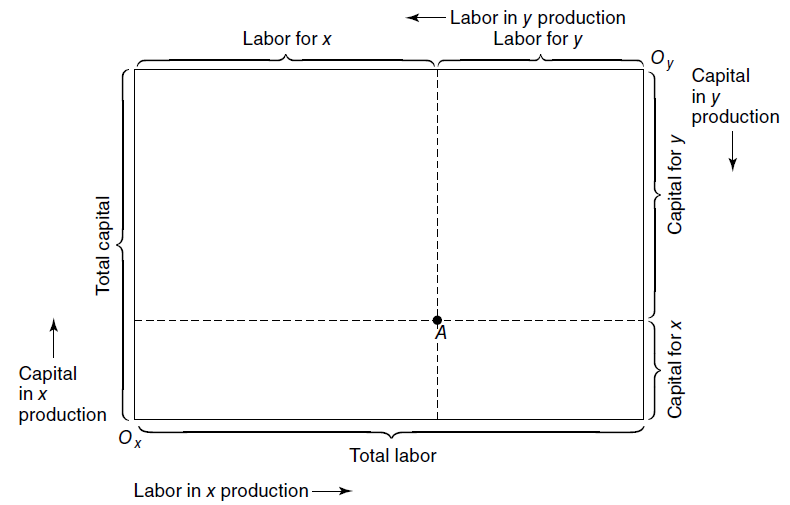
\includegraphics[width=0.70\linewidth]{Imagens/a3i1.png}
\end{figure}

\begin{figure}[H]
    \centering
    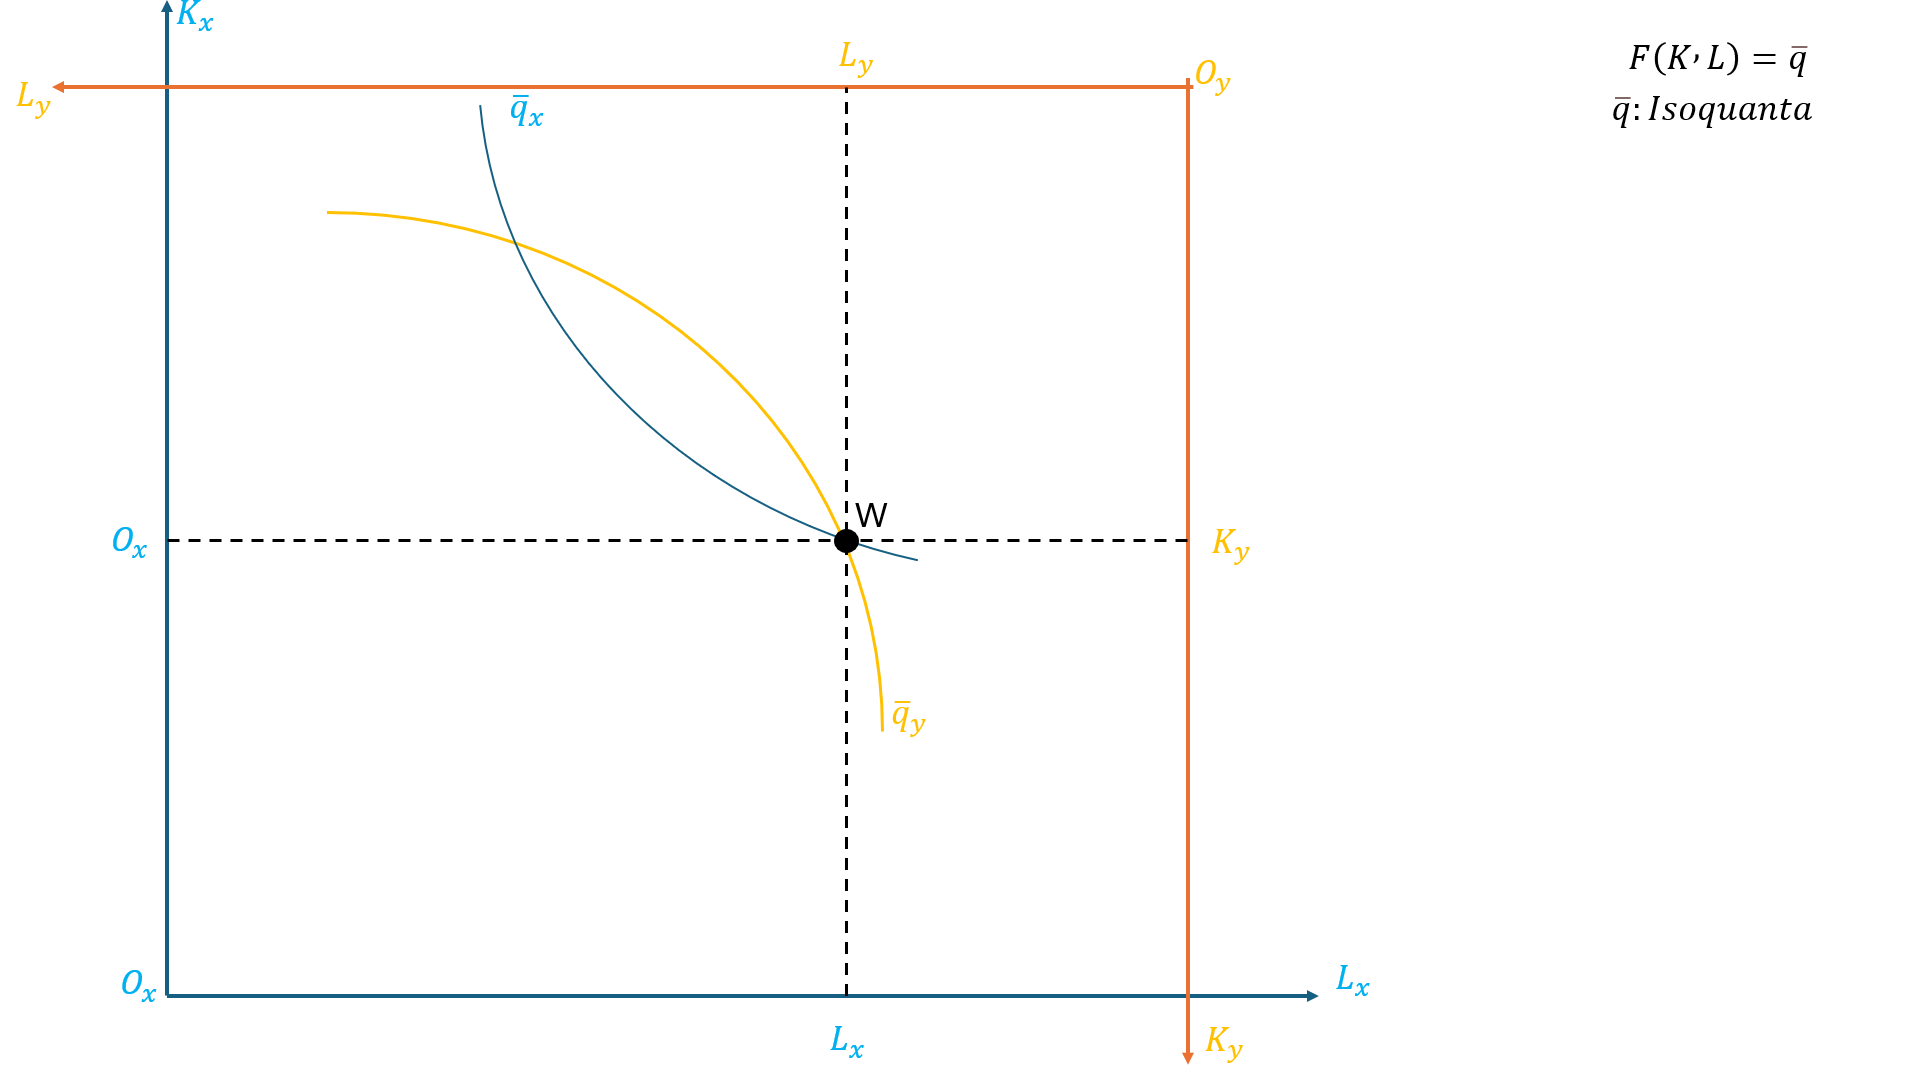
\includegraphics[width=0.7\linewidth]{Imagens/a5i1.png}
\end{figure}

Apesar de Z ser um ponto em que eu consigo produzir mais dos dois bens nesse país, não necessariamente o bem estar aumentou, em termos de eficiência produtiva, sim Z é melhor que W, mas temos que olhar para o olhar do consumidor também.

\begin{figure}[H]
    \centering
    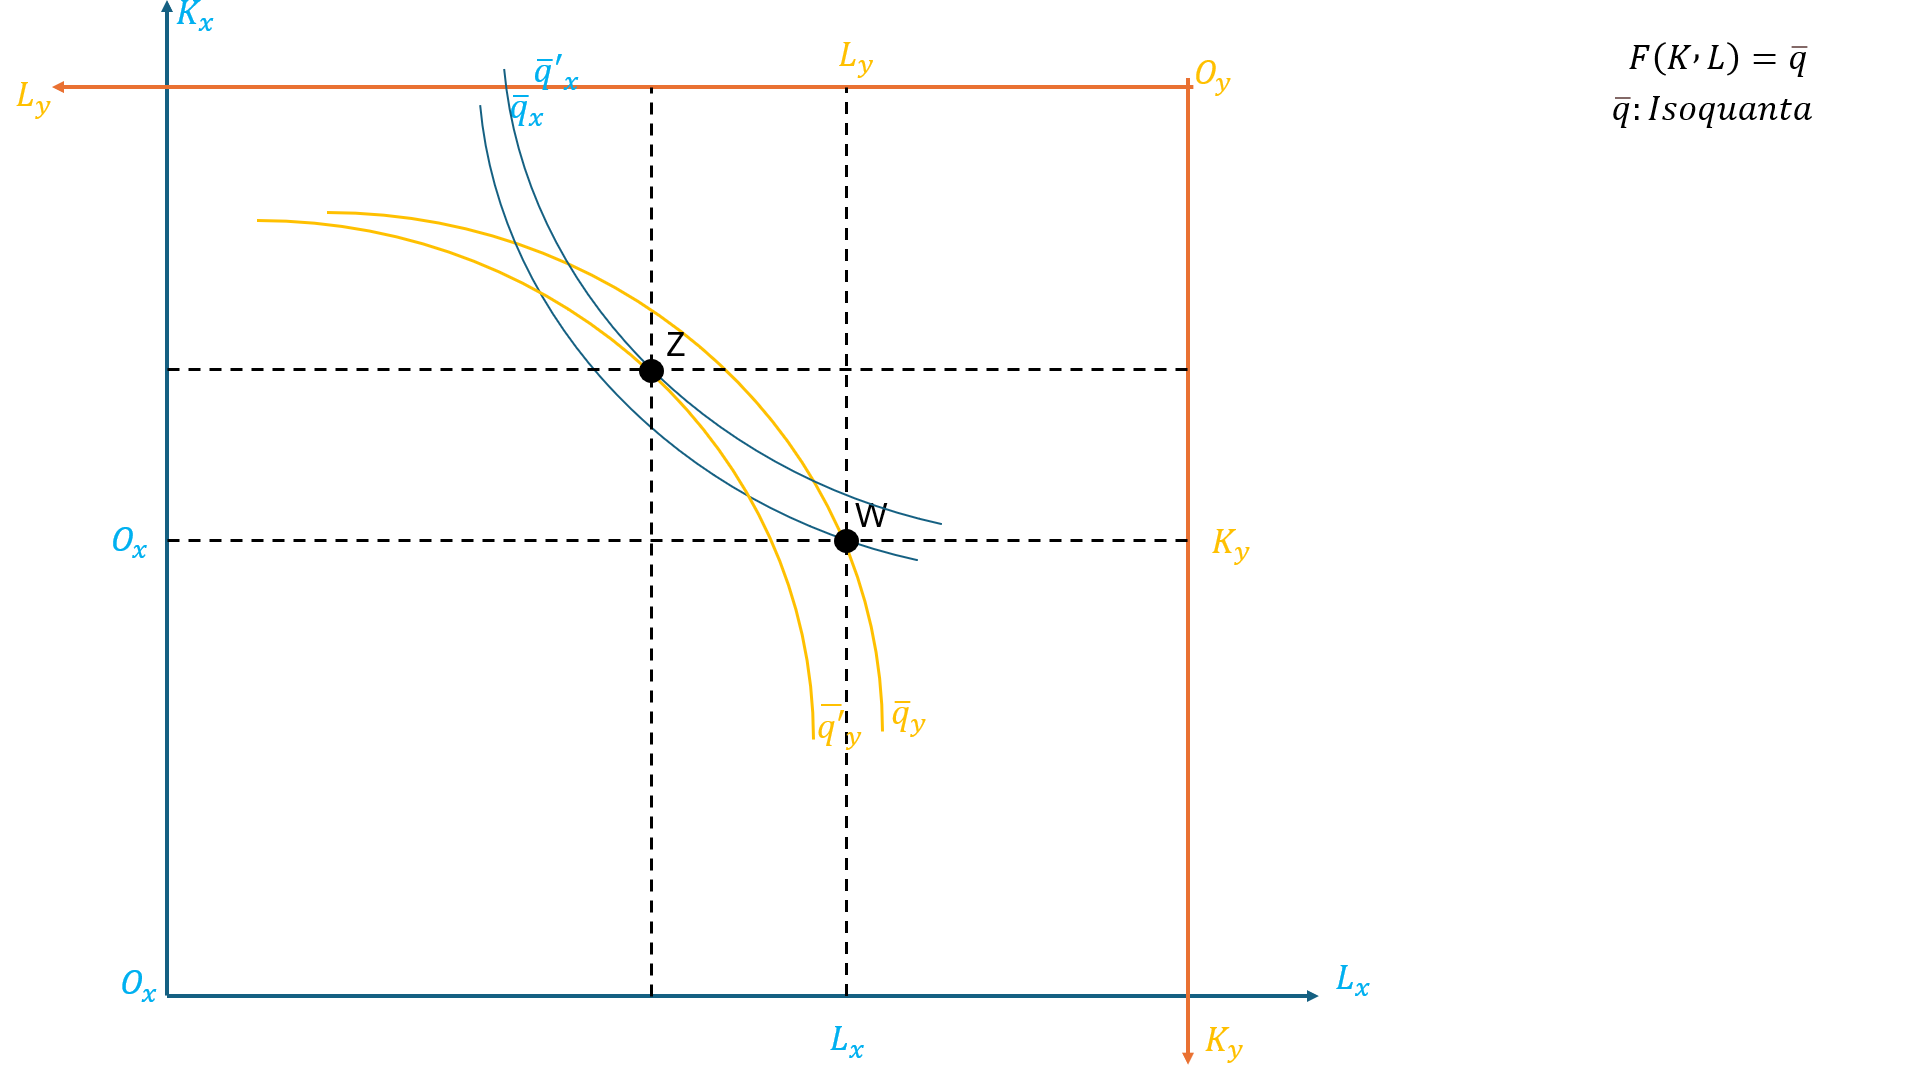
\includegraphics[width=0.7\linewidth]{Imagens/a5i2.png}
\end{figure}

Utilizaremos o mapa de \textbf{isoquantas} para representar a quantidade produzida de cada bem: \begin{itemize}
    \item Isoquantas estão associadas à tecnologias das firmas
    \item As isoquantas para o bem manufaturado utilizam \(O_x\) como origem
\end{itemize} 

O ponto A (da figura abaixo) é classificado como ineficiente\begin{itemize}
    \item É possível aumentar a produção dos bens apenas realocando os insumos 
\end{itemize}

\begin{figure}[H]
    \centering
    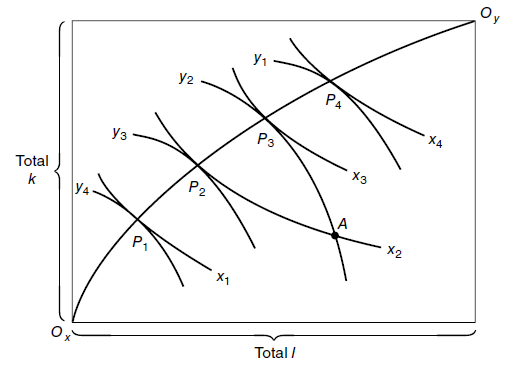
\includegraphics[width=0.70\linewidth]{Imagens/a3i2.png}
\end{figure}


Ligando todos os pontos eficientes, temos a "curva de contrato" só que dos produtores, aqui olhamos como combinamos capital e trabalho para produzir o máximo de bens. Todos os pontos sobre a curva de contrato são os pontos de produção eficiente.
\begin{figure}[H]
    \centering
    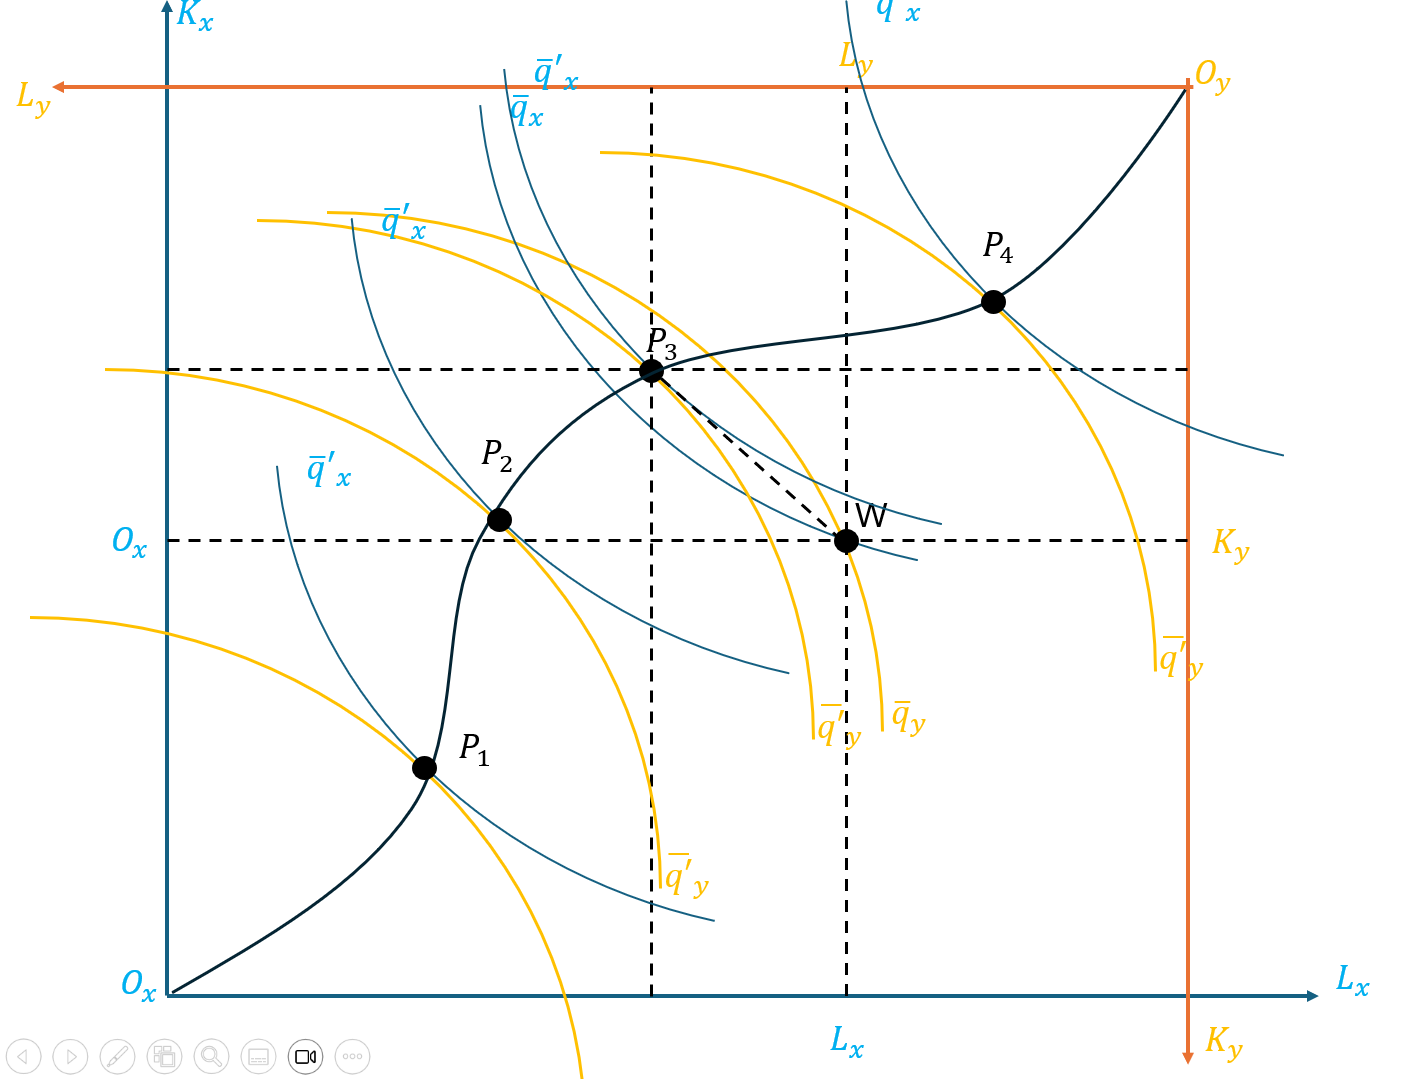
\includegraphics[width=0.7\linewidth]{Imagens/a5i3.png}
\end{figure}

Porém ficar olhando as caixas de Edgeworth é muito complexo, ainda mais quando formos olhar para o consumidor também, por isso que iremos olhar para a quantidade de bens finais produzidas.

\subsection{\textbf{Fronteira de Possibilidade de Produção (\textit{FPP})}}

\textbf{Conjunto Eficiente de Produção}\begin{itemize}
    \item As alocações eficientes ocorrem quando as isoquantas são tangentes entre si
    \item TMST é igual na produção de bens agrícolas e manufaturados 
    \item Podemos, então, construir a Fronteira de Possibilidades de Produção \textbf{FPP}
\end{itemize}

\begin{figure}[H]
    \centering
    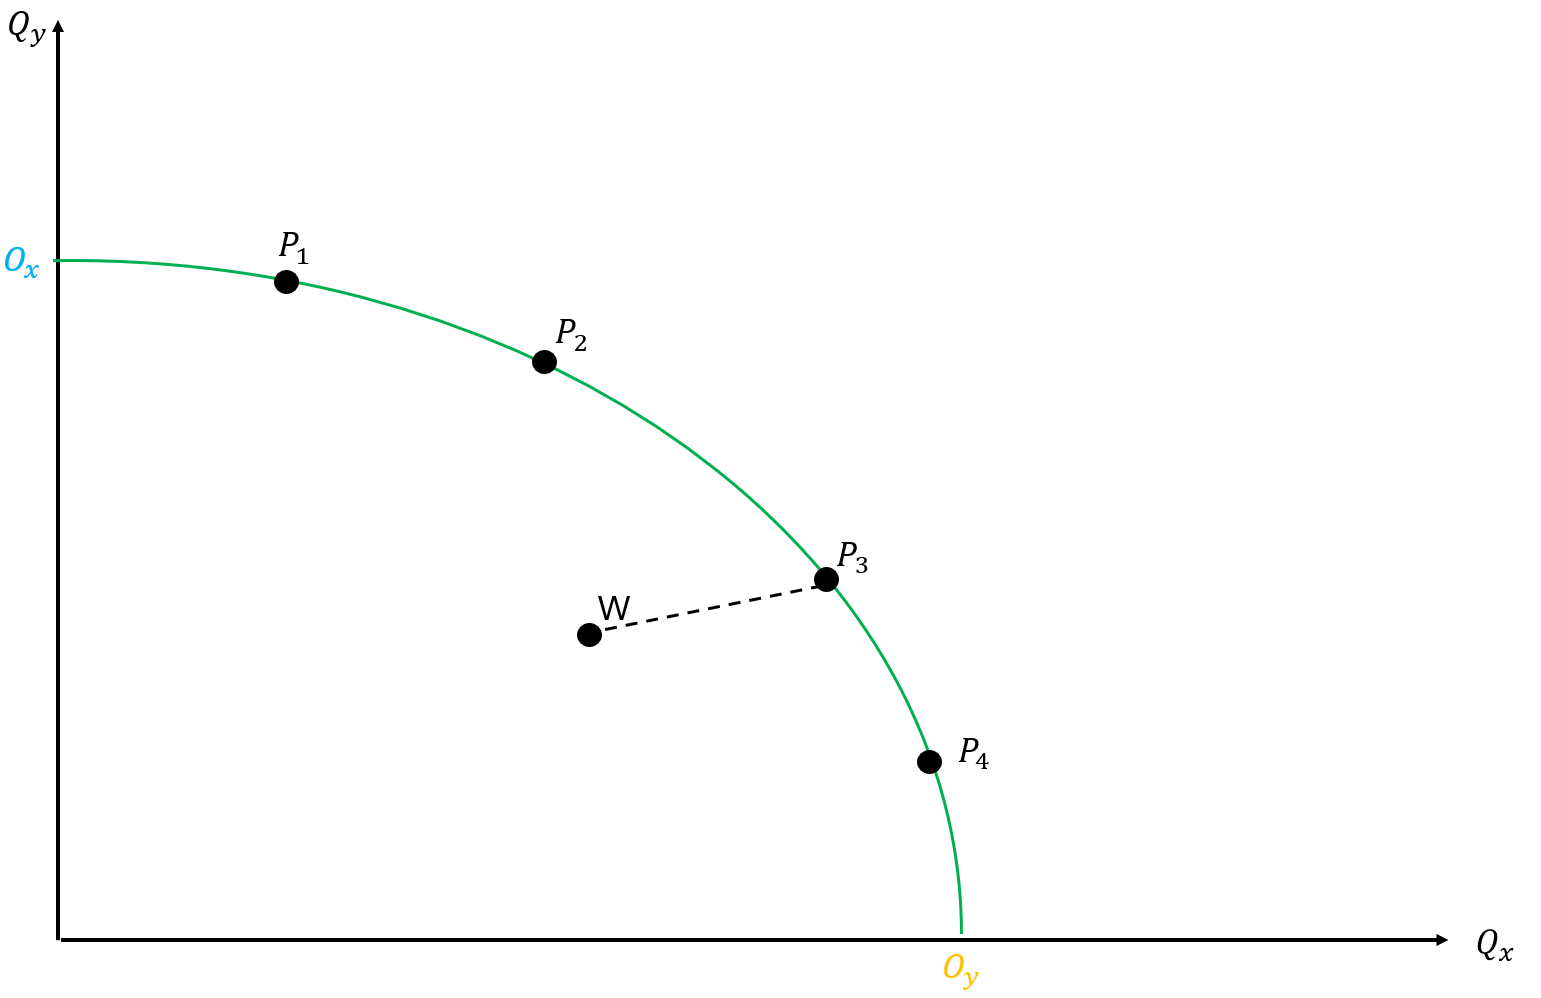
\includegraphics[width=0.7\linewidth]{Imagens/a5i4.png}
\end{figure}

\begin{figure}[H]
    \centering
    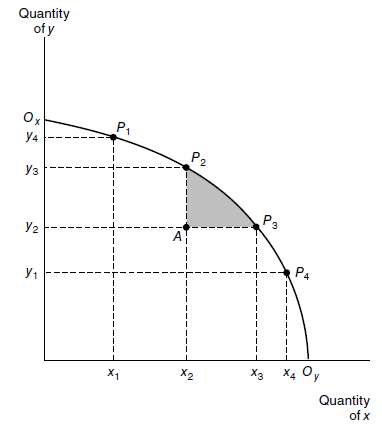
\includegraphics[width=0.70\linewidth]{Imagens/a3i3.png}
\end{figure}

A \textbf{FPP} representa as combinações possíveis de bens finais que podem ser produzidas dadas as quantidades de insumos.

A fronteira desse conjunto corresponde às combinações \textbf{eficientes de produção}

Os pontos dentro do conjunto são factíveis, mas ineficientes.

\textbf{Taxa Marginal de Trasnformação(\textit{TMT})} A inclinação da \textbf{FPP} representa a taxa em que a produção de um bem pode ser trocada pela produção de outro bem \[TMT = -\frac{dy}{dx}\].

\begin{figure}[H]
    \centering
    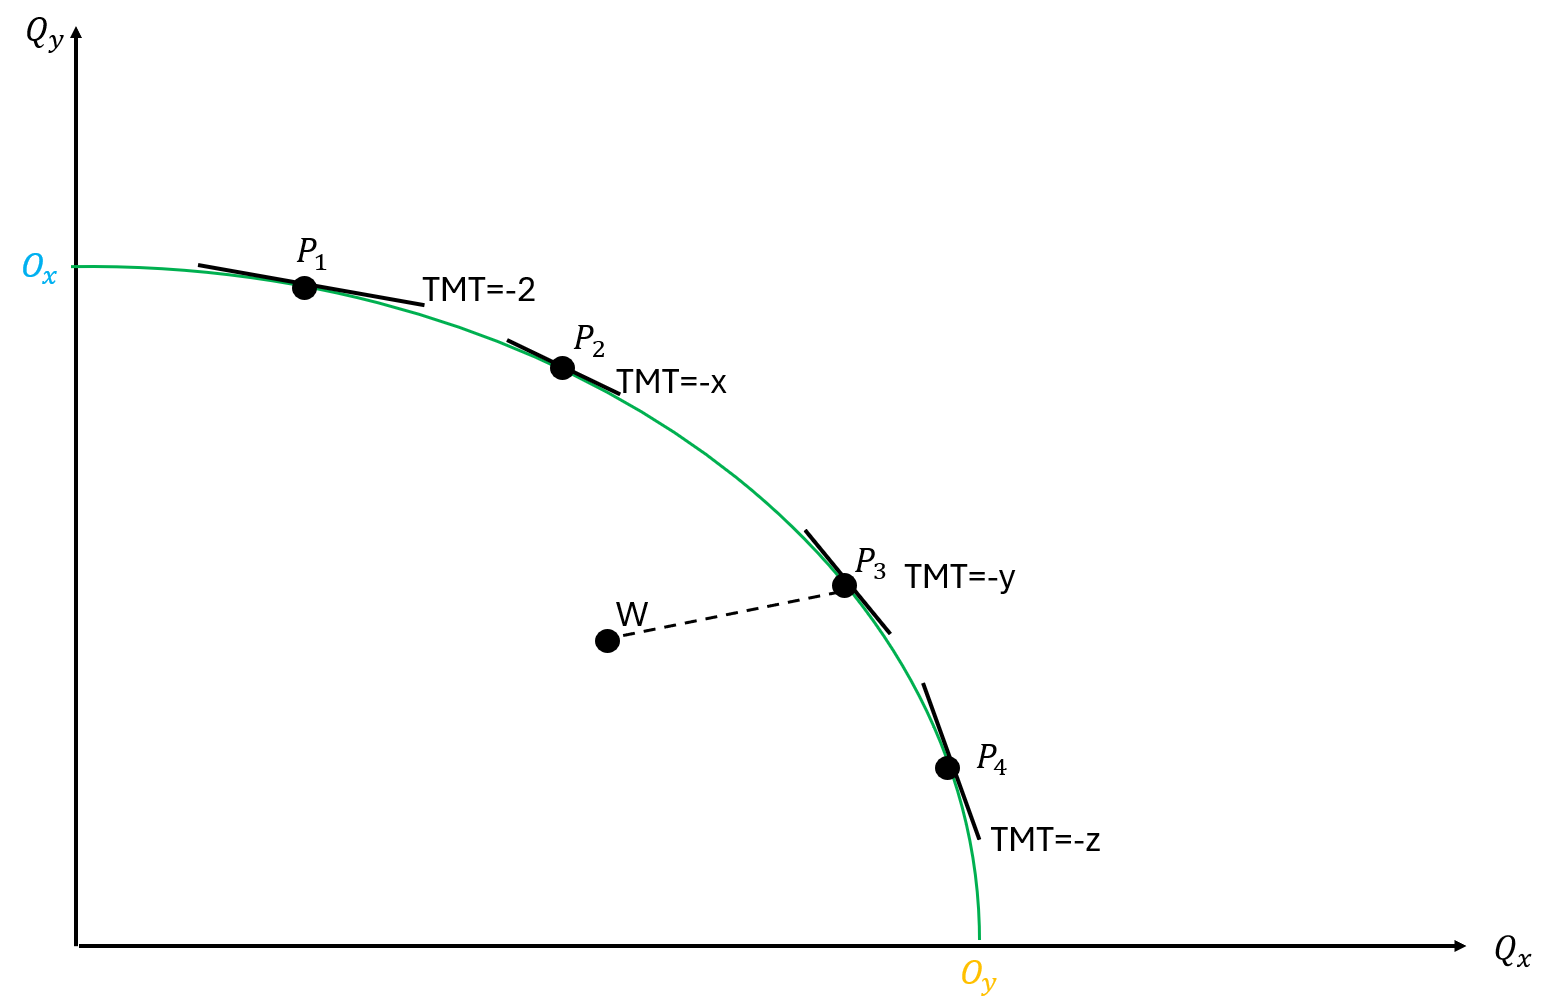
\includegraphics[width=0.7\linewidth]{Imagens/a5i5.png}
\end{figure}

A \textbf{FPP} apresentada anteriormente possui uma \textbf{TMT crescente}.

Por que esse formato côncavo da \textbf{FPP} caracteriza muitos processos produtivos?\begin{itemize}
    \item Retorno decrescentes de escala 
    \item Insumos especializados 
    \item Intensidade no uso dos fatores 
\end{itemize}

Cuidado! Apesar de muito comum, a \textbf{FPP} nem sempre será côncava(mais sobre isso a frente).

\subsubsection{\textbf{FPP-Exercício}}
Por simplicidade, suponha que os setores agrícola e de manufatura utilizem apenas o fator trabalho: 
\[
q_x=f(L_x)=L_x^{1/2}
\]
\[
q_y=f(L_y)=L_y^{1/2}
\]

A oferta total de trabalho é dada por $L_A+L_M=100$. Encontro uma expressão para a \textbf{FPP} e \textbf{TMT} associada.\begin{enumerate}
    \item \(q_x=f(L_x)=L_x^{1/2}\rightarrow L_x=q_x^2\)
    \item \(q_y=f(L_y)=L_y^{1/2}\rightarrow L_y=q_y^2\)
    \item \(q_x^2+q_y^2=100\rightarrow q_y=(q_x^2-100)^{1/2}\)
    \item 
\begin{figure}[H]
    \centering
    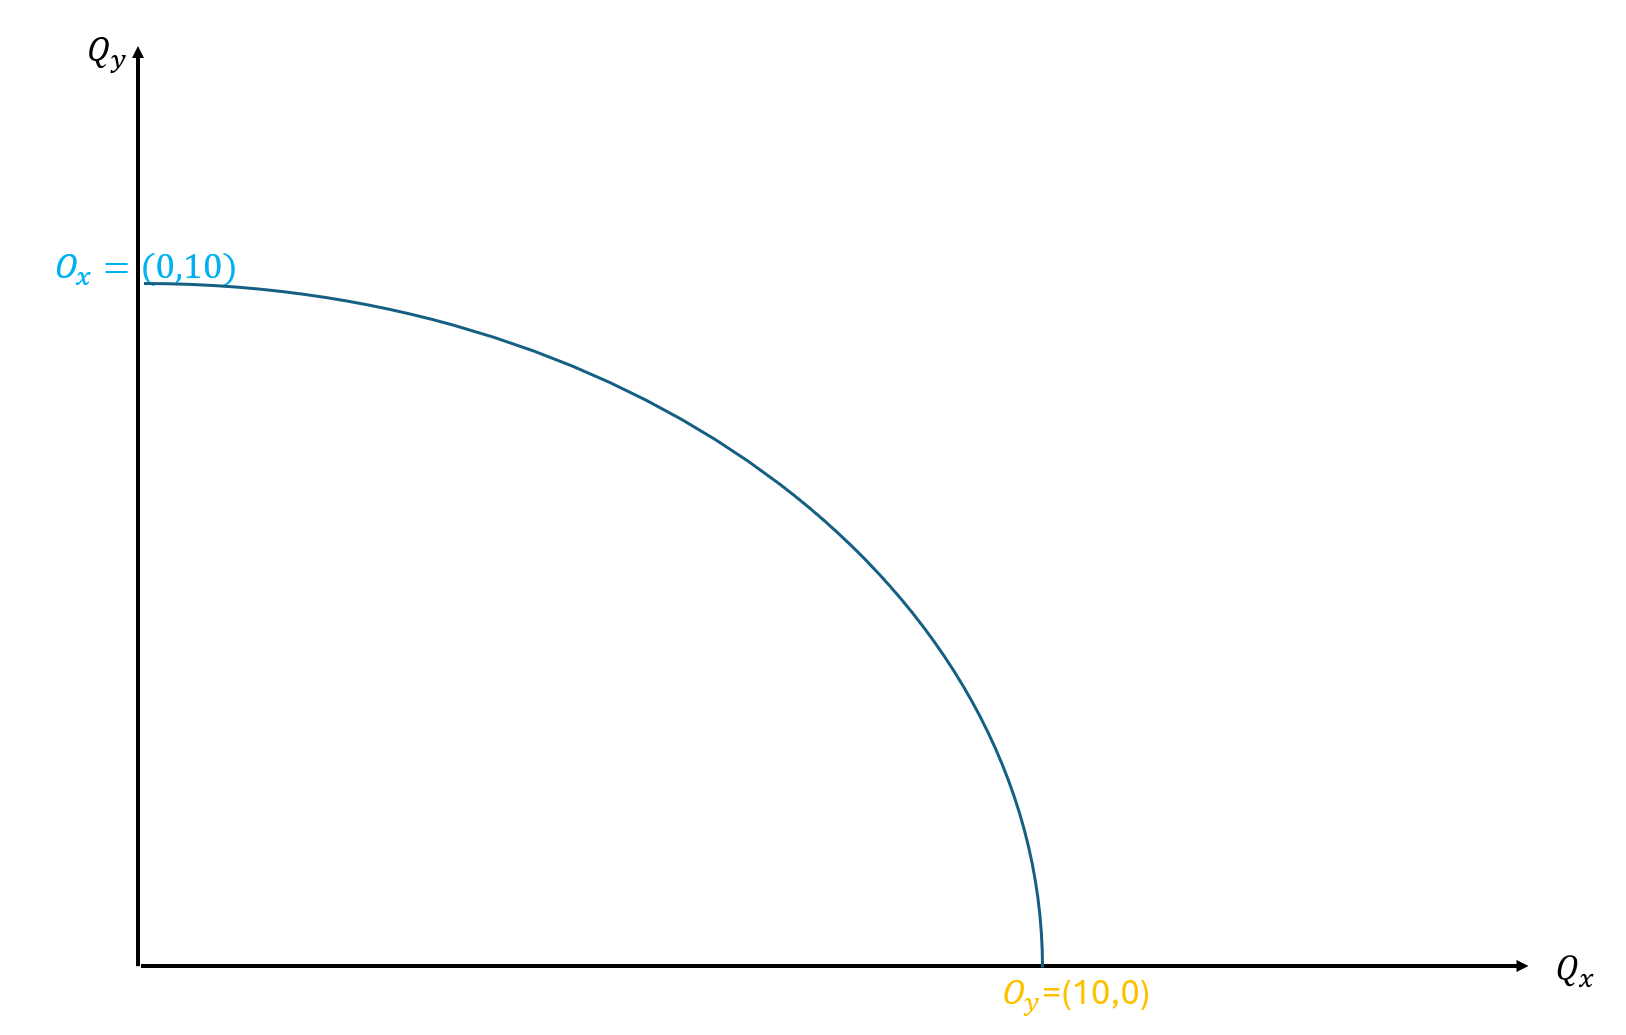
\includegraphics[width=0.7\linewidth]{Imagens/a5i6.png}
\end{figure}
    \item \(TMT=\frac{dQ_y}{dQ_x}=\frac{1}{2}(q_x^2-100)^{-1/2}(-2q_x)=-\frac{q_x}{(q_x^2-100)^{1/2}}=-\frac{q_x}{q_y}\)
    \item \(2q_x\cdot dq_x+2q_y\cdot dq_y=0\rightarrow q_x\cdot dq_x+q_y\cdot dq_y=0 \rightarrow \frac{dq_y}{dq_x}=-\frac{q_x}{q_y}\)
\end{enumerate}

Note que os pontos (10,0) e (0,10) são eficientes, mas o ponto (5,5) não.

\subsection{\textbf{Determinação dos Preços de Equilíbrio}}
A restrição orçamentária da produção:
\[
P_xx+P_yy=I=P_xQ_x+P_yQ_y
\]

Agora que já construímos a \textbf{FPP}, precisamos analisar como os preços de equilíbrio dos bens finais são determinados.

Lembre-se que a \textbf{FPP} mostra todas as combinações efientes de \textbf{produção}.

Precisamos determinar a demanda por esses bens a partir das preferências dos consumidores.

Por simplicidade, assuma uma função de utilidade agregada representada por curvas de indiferença comunitárias(mais detalhes a frente)

\begin{figure}[H]
    \centering
    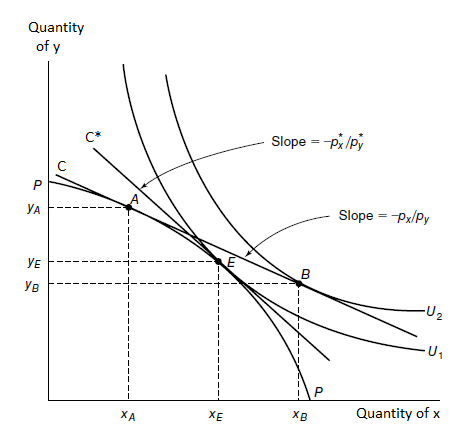
\includegraphics[width=0.70\linewidth]{Imagens/a3i4.png}
\end{figure}

\begin{figure}[H]
    \centering
    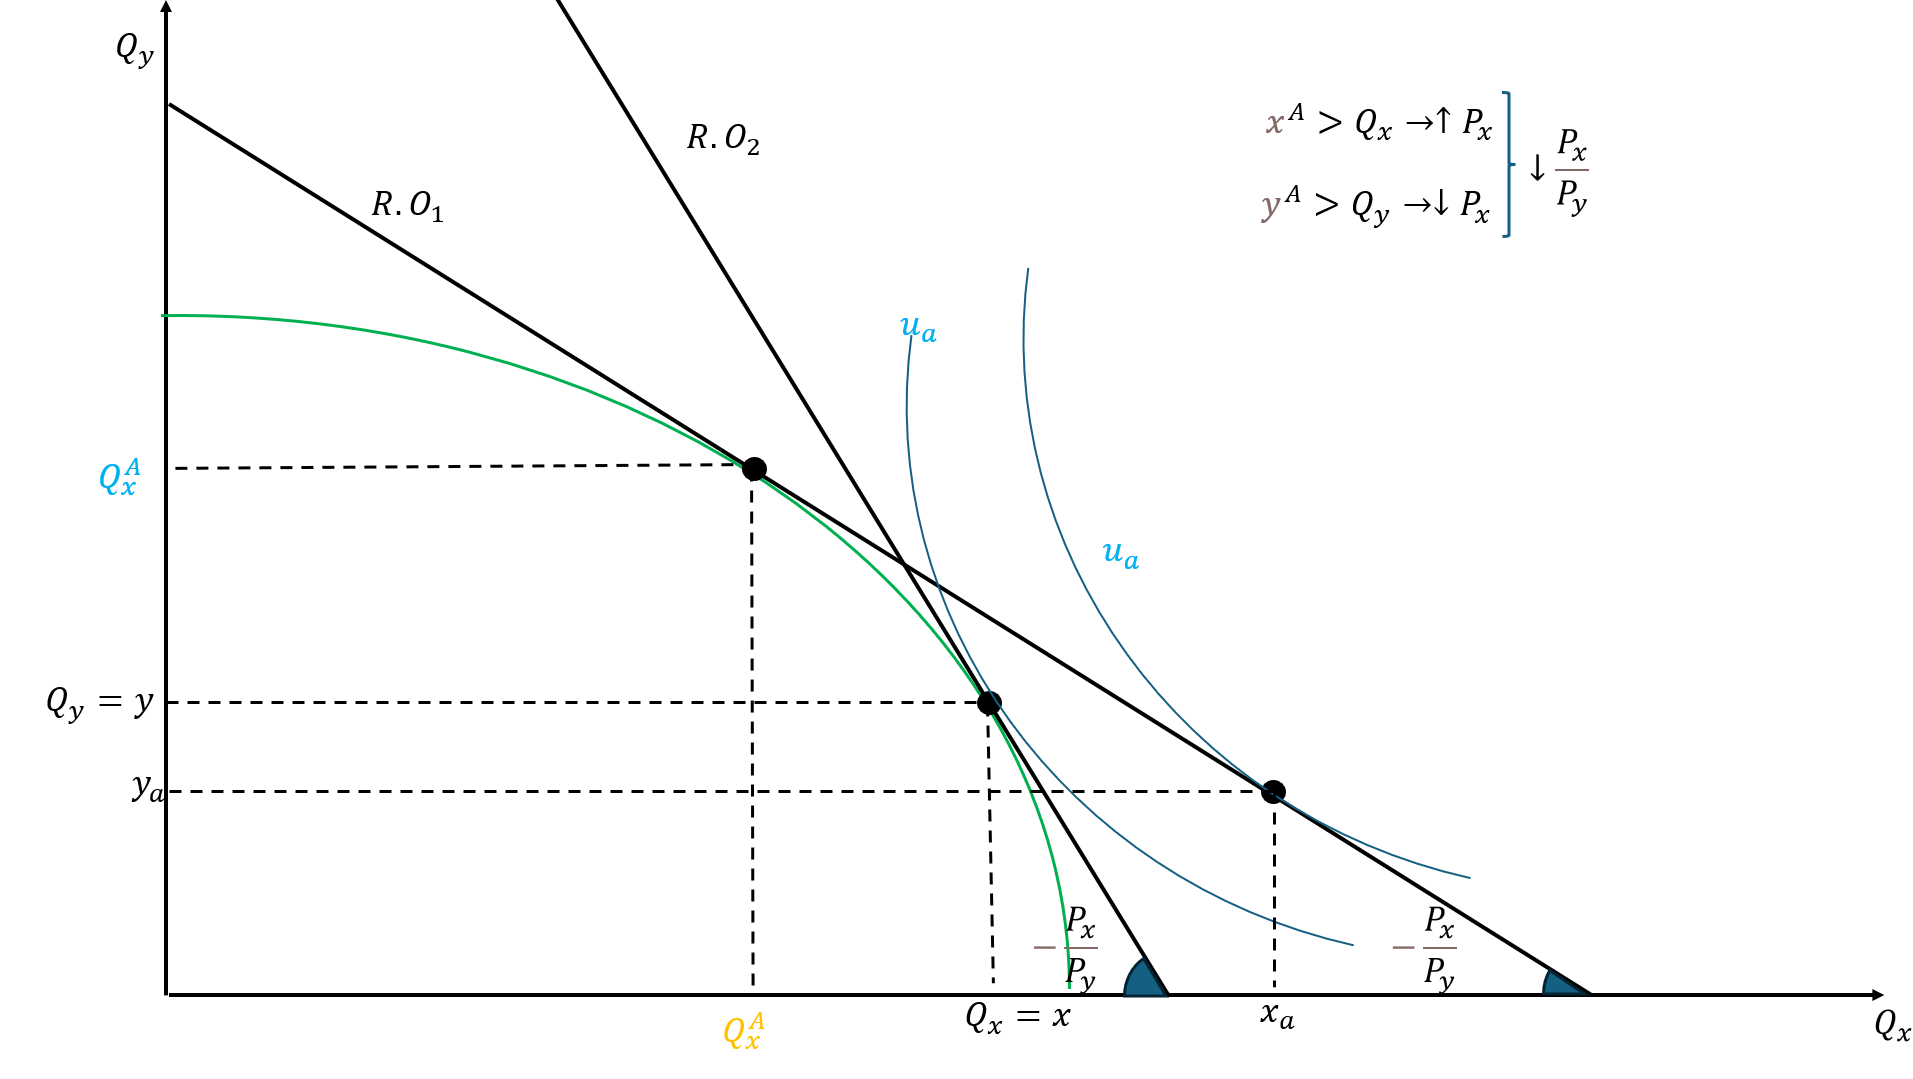
\includegraphics[width=0.7\linewidth]{Imagens/a5i7.png}
\end{figure}

Condições de equilíbrio\begin{itemize}
    \item TMT = \(\frac{P_x}{P_y}\)
    \item TMS = \(\frac{P_x}{P_y}\)
    \item TMS = TMT = \(\frac{P_x}{P_y}\)
    \item \(q_x=x\) e \(q_y=y\)
\end{itemize}

Se os preços de equilíbrio são $p_x \ e\ p_y$, então a restrição orçamentária da sociedade é C\begin{itemize}
    \item a produção será $(x_A,y_A)$
    \item os consumidores demandarão$(x_B,y_B)$
\end{itemize}

Teremos excesso de demanda para $x$ e excesso de oferta para $y$\begin{itemize}
    \item o preço de $x$ subirá 
    \item o preço de $y$ cairá 
\end{itemize}

O equilíbrio ocorrerá no ponto $(x_E,y_E)$, onde a curva de indiferença é tangente à \textbf{FPP}$\rightarrow$\textbf{TMT=TMS}

\subsubsection{\textbf{Determinação dos Preços de Equilíbrio - Exercício}}

Voltando ao exemplo anterior 
\[
q_M=f(L_M)=L_M^{1/2}
\]
\[
q_A=f(L_A)=L_A^{1/2}
\]
\[
L_A+L_M=100
\]

Supondo que as preferências da sociedade sejam representadas por $u(x,y)=x^{1/2}y^{1/2}$

Encontre os equilíbrios(preços e quantidades)\begin{enumerate}
    \item \(TMS=\frac{y}{x}\)
    \item \(TMT=\frac{q_x}{q_y}\)
    \item \(TMS=TMT\rightarrow \frac{y}{x}=\frac{q_x}{q_y}\)
    \item \(x=q_x \ ; \ y=q_y \)
    \item \(\frac{q_y}{q_x}=\frac{q_x}{q_y}=q_x^2=q_y^2\rightarrow q_x=q_y\)
    \item \(q_x^2+q_x^2=100 \rightarrow q_x^2=50 \rightarrow q_x=\sqrt{50} \rightarrow q_y=\sqrt{50}\)
    \item \(\frac{P_x}{P_y}\frac{\sqrt{50}}{\sqrt{50}}=1\)
    \begin{figure}[H]
        \centering
        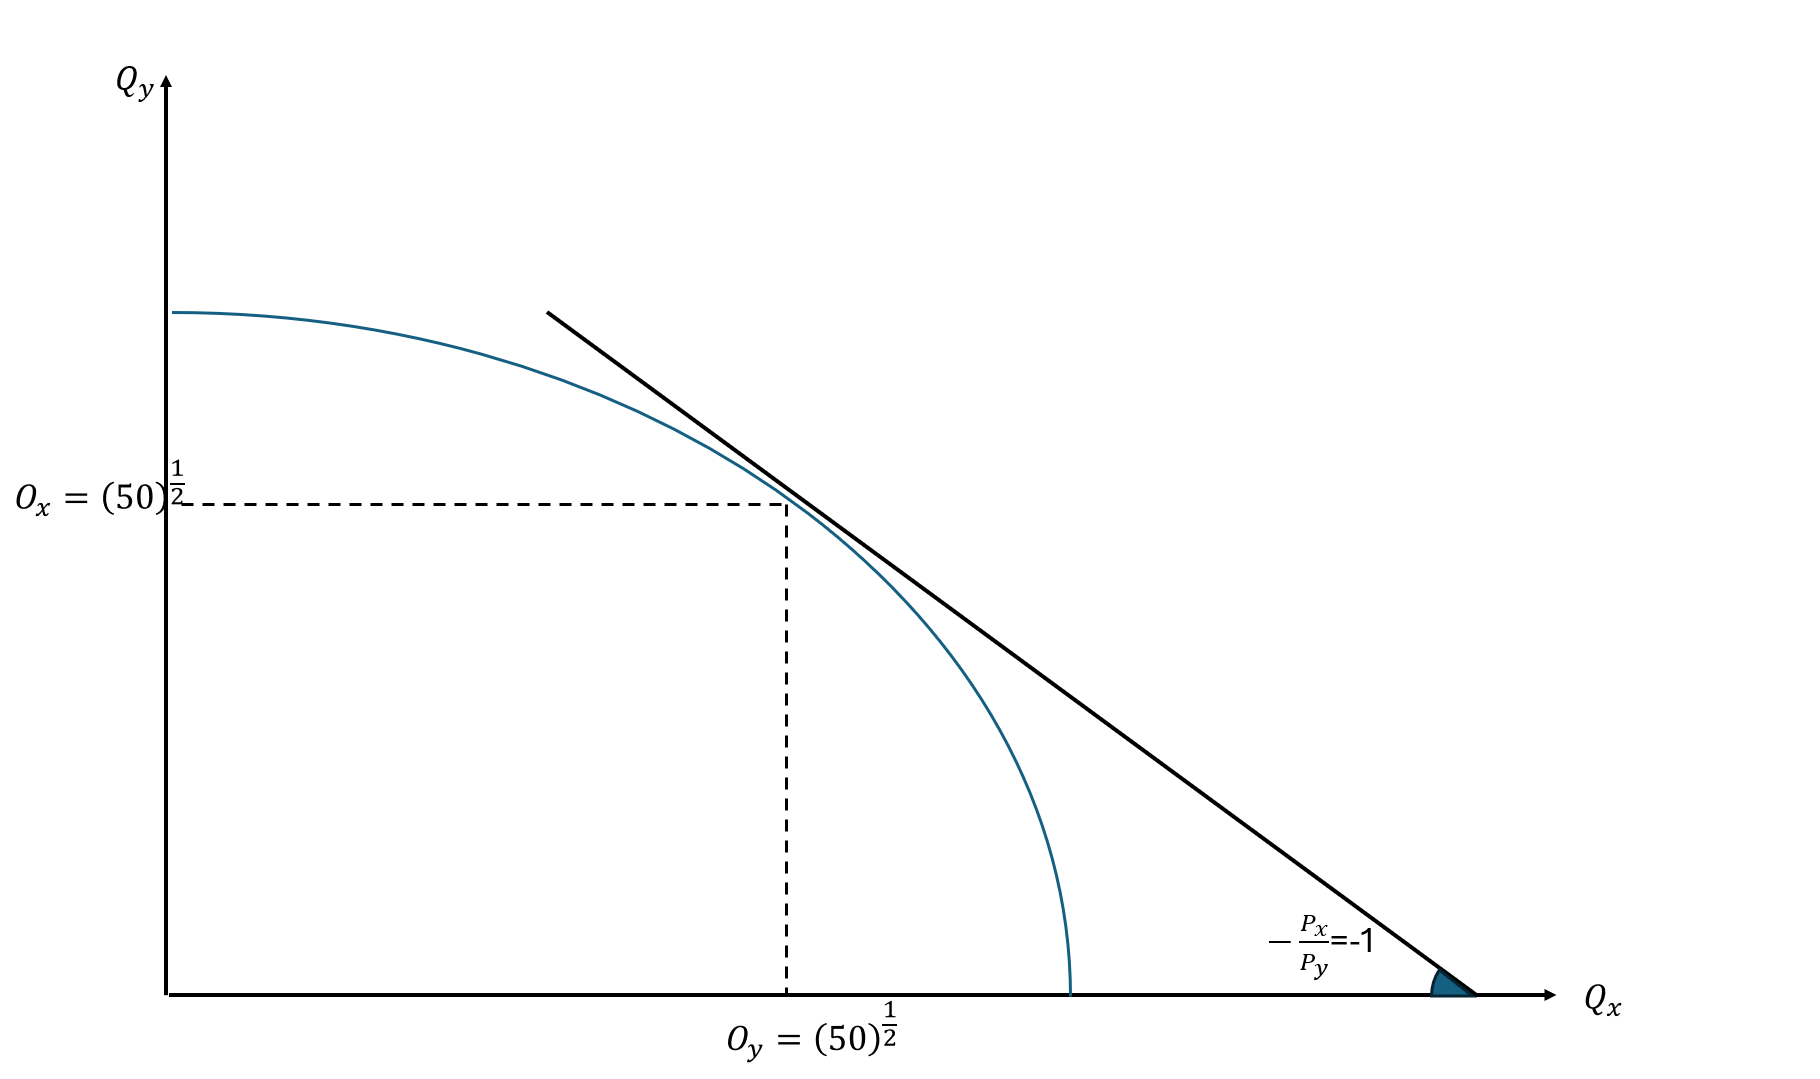
\includegraphics[width=0.7\linewidth]{Imagens/a6i1.png}
    \end{figure}
\end{enumerate}

Todos os preços são \textbf{endógenos} dentro do modelo. Os elementos \textbf{exógenos} são as preferências e as tecnologias de produção.

Mudanças nas preferências ou nas tecnologias levam a um novo equilíbrio de preços relativos e de produção/consumo.

A existência do equilíbrio depende das seguintes hipóteses\begin{itemize}
    \item Ausência de custos de transação 
    \item Informação completo 
    \item Ausência de externalidades
    \item Preferências racionais, contínuas e estritamente convexas 
    \item Ausência de poder de mercado
\end{itemize}

\subsection{\textbf{Preços Competitivos e Eficiência}}

Além do equilíbrio de oferta e demanda, quais outras propriedades estão presentes no sistema competitivo de alocação de recuros?

Para responder essa questão, vamos voltar às três dimensões de eficiência do início da aula \begin{enumerate}
    \item Eficiência alocativa
    \item Eficiência produtiva 
    \item Eficiência do mix de produtos
\end{enumerate}

\subsection{\textbf{Eficiência Alocativa}}

Cada consumidor $i$, $i=\{1,2\}$ toma os preços como dados e maximiza a sua utilidade sujeito a uma restrição orçamentária 
\[
\max_{x,y} u_i(x_i, y_i) \quad \text{s.a.} \quad p_x x_i + p_y y_i = l_i
\]

Note que os consumidores se deparam com os mesmos preços dos bens finais.

Resolvendo as condições de primeira ordem
\[
TMS_1=TMS_2=\frac{p_x}{p_y}
\]

Portanto, o equilíbrio de mercado satisfaz a eficiência alocativa

\subsection{\textbf{Eficiência Produtiva}}

Cada firma $j$, $j=\{A,M\}$ toma os preços dos bens finais e dos insumos como dados e maximiza o lucro
\[
\max_{K_j,L_j}=p_jF_j(K_j,L_j)-wL_j-rK_j
\]

Note que as firmas se deparam com os mesmo preços dos insumos .

Resolvendo as condições de primeira ordem 
\[
TMST_A=TMST_M=\frac{w}{r}
\]

Portanto, o equilíbrio de mercado satisfaz a eficiência produtiva. 

\subsection{\textbf{Eficiência do Mix de Produtos}}
É possível que o mercado tenha usado K e L  de maneira eficiente na produção dos bens agrícola e manufaturado.

E se o mercado produzir um mix de produtos que não corresponde às preferências da sociedade?

Por exemplo, muitos produtos agrícolas e poucos produtos manufaturados ou vice-versa?

Qual é a condição necessária para garantir que as quantidades corretas dos bens sejam produzidas?\begin{itemize}
    \item Tangência entre a curva de indiferença comunitária e a \textbf{FPP}
\end{itemize}

\begin{figure}[H]
    \centering
    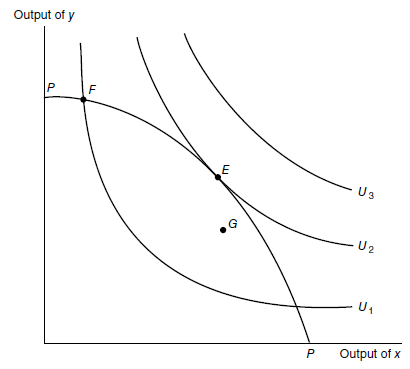
\includegraphics[width=0.70\linewidth]{Imagens/a3i5.png}
\end{figure}

Suponha que a \textbf{FPP} posssa ser escrita por uma função implícita da forma $T(x,y)=0$. Então,
\[
\max_{x,y}y(x,y) \quad \text{s.a.} \quad T(x,y)=0
\]

Resolvendo as condições de primeira ordem 
\[
TMS=\frac{\partial T/\partial x}{\partial T/\partial y}=-\frac{dy}{dx}=TMT
\]

Isso implica que, no equilíbrio, $TMT=\frac{p_x}{p_y}$

\begin{figure}[H]
    \centering
    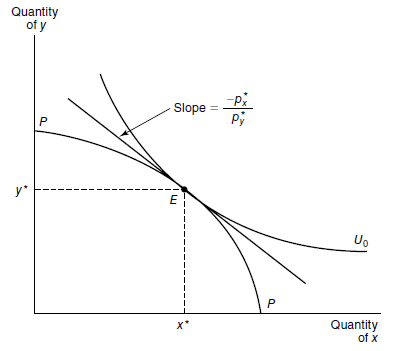
\includegraphics[width=0.70\linewidth]{Imagens/a3i6.png}
\end{figure}

\subsection{\textbf{Resumo}}

Mostramos que o equilíbrio de mercado competitivo satisfaz simultaneamente todos os critérios de eficiência

Dadas as quantidades de insumos, as preferências dos consumidores e as tecnologias das firmas, existe um vetor de preços tal que

\begin{itemize}
    \item Os mercados de bens finais e de insumos se equilibram (não há excesso de oferta ou demanda)
    \item Todos os ganhos do comércio entre consumidores e de realocação de recursos entre os setores serão esgotados
\end{itemize}

Portanto, o equilíbrio competitivo será eficiente no sentido de Pareto.

\begin{figure}[H]
    \centering
    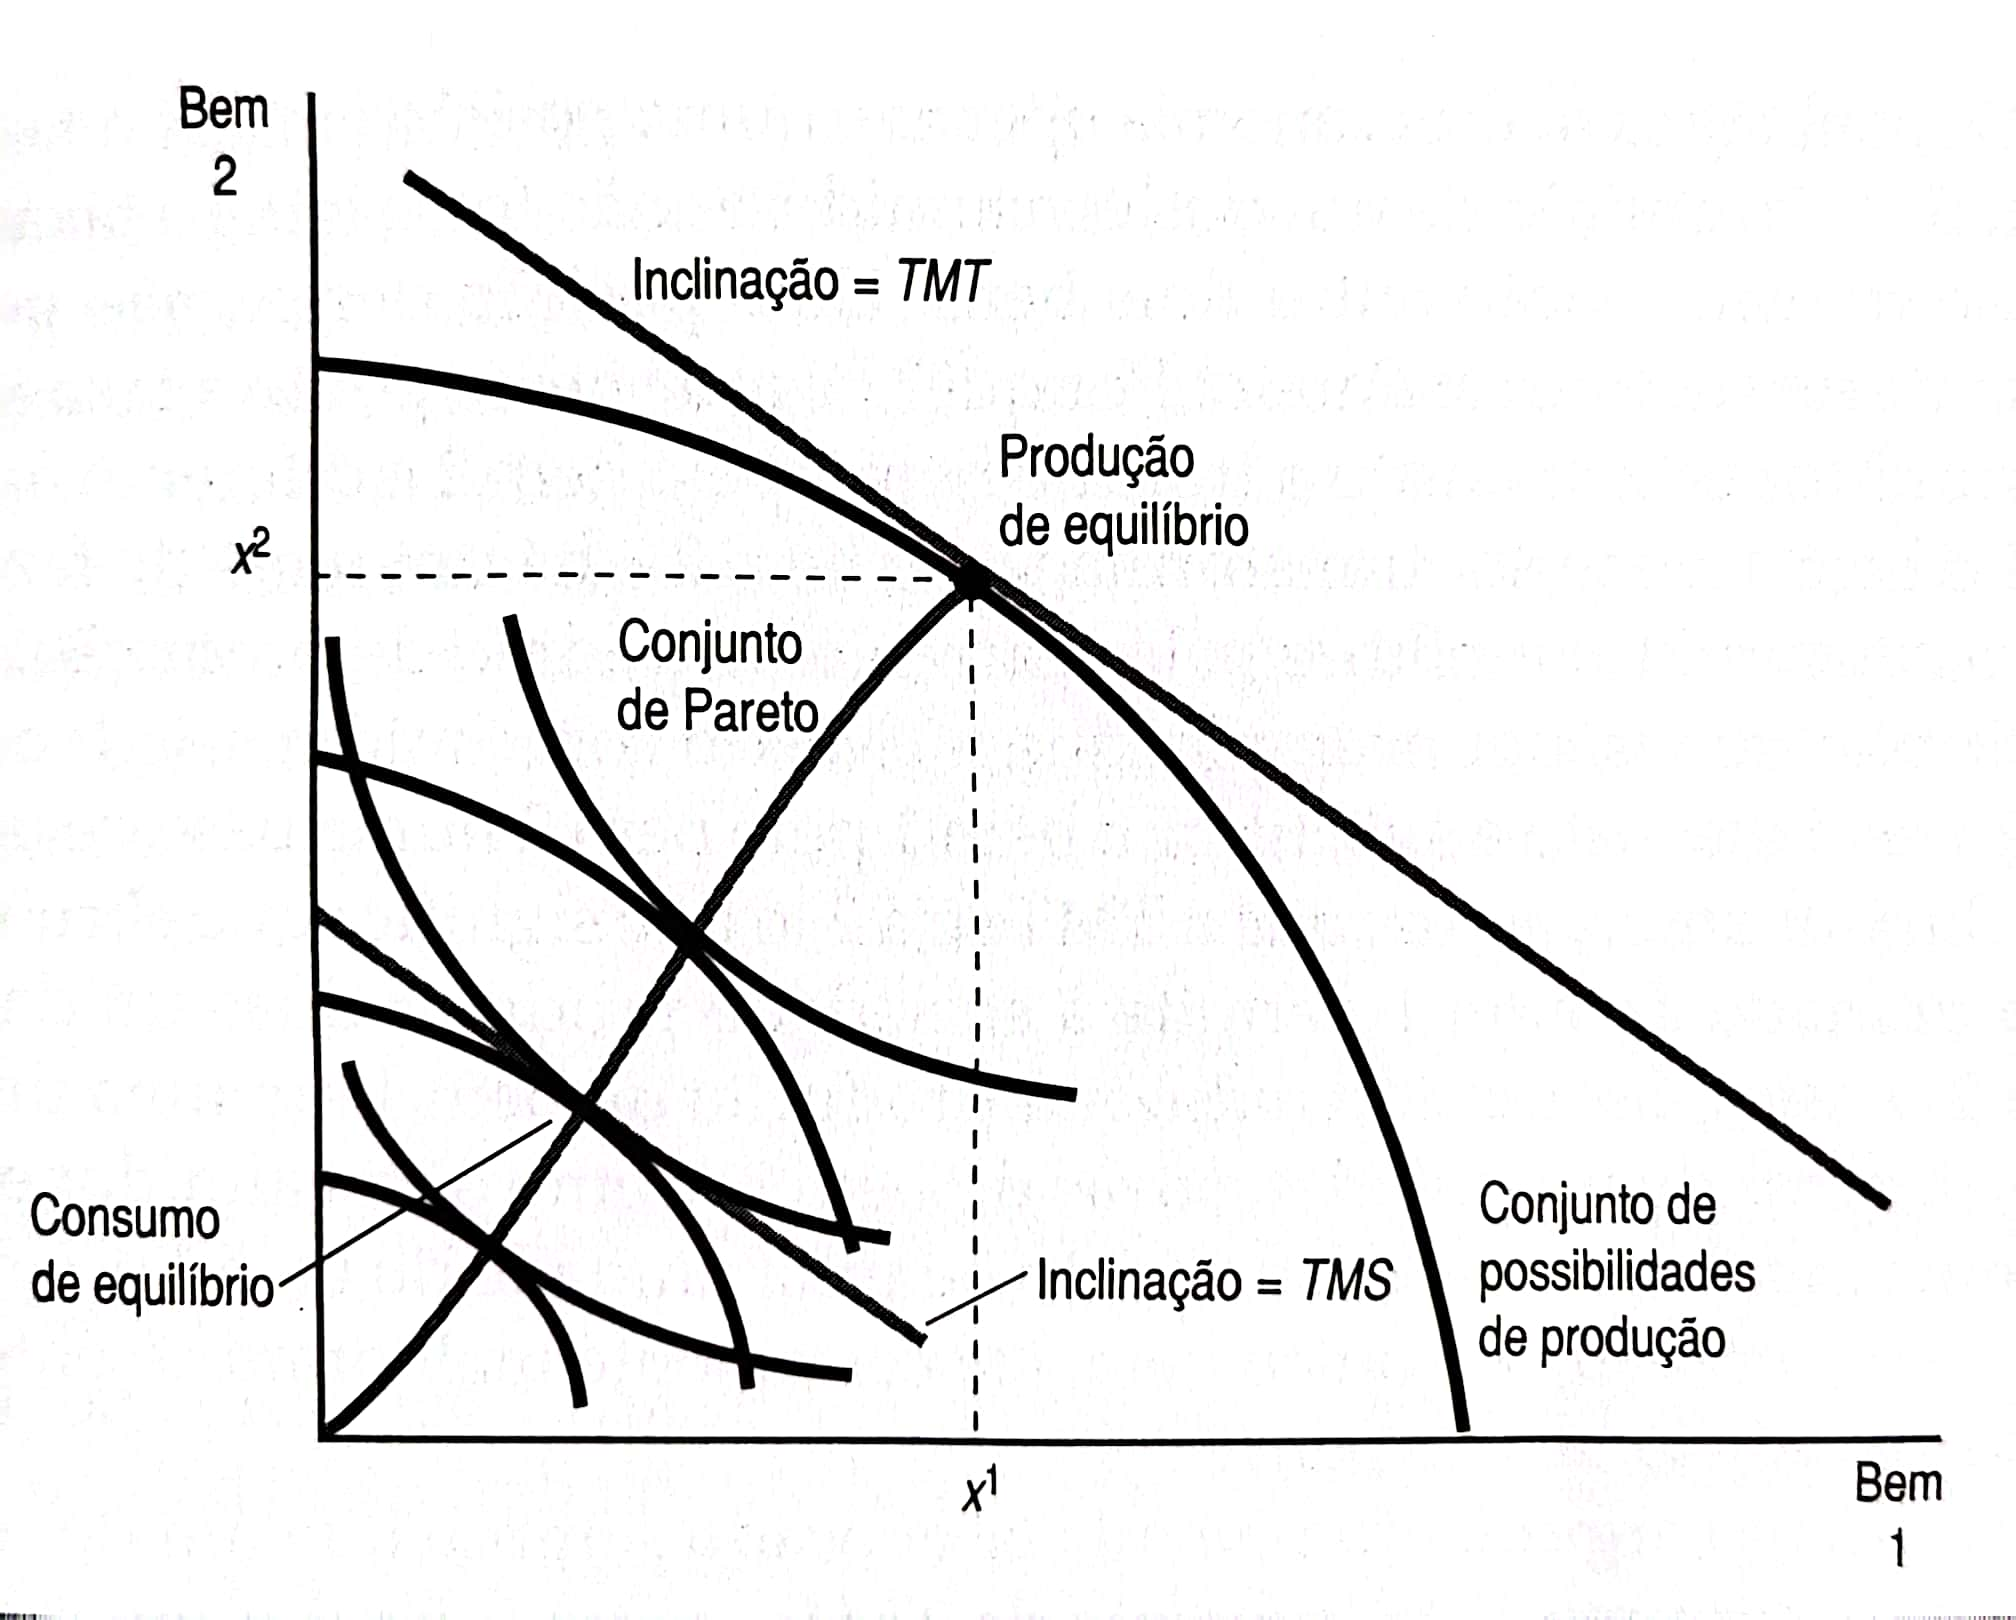
\includegraphics[width=0.70\linewidth]{Imagens/a3i7.png}
\end{figure}

\subsection{\textbf{Aplicação: Comércio Internacional}}

Vamos usar o arcabouço que acabamos de construir para analisar de maneira simplificada o impacto de uma abertura comercial

Considere uma pequena economia aberta inicialmente em autarquia (sem comércio)

Suponha que esse país retire todas as barreiras comerciais e passe a comercializar com o resto do mundo

Considere ainda que o preço relativo do bem x  no mercado internacional seja menor que no mercado doméstico

Represente graficamente essa situação e explique intuitivamente
\begin{figure}[H]
    \centering
    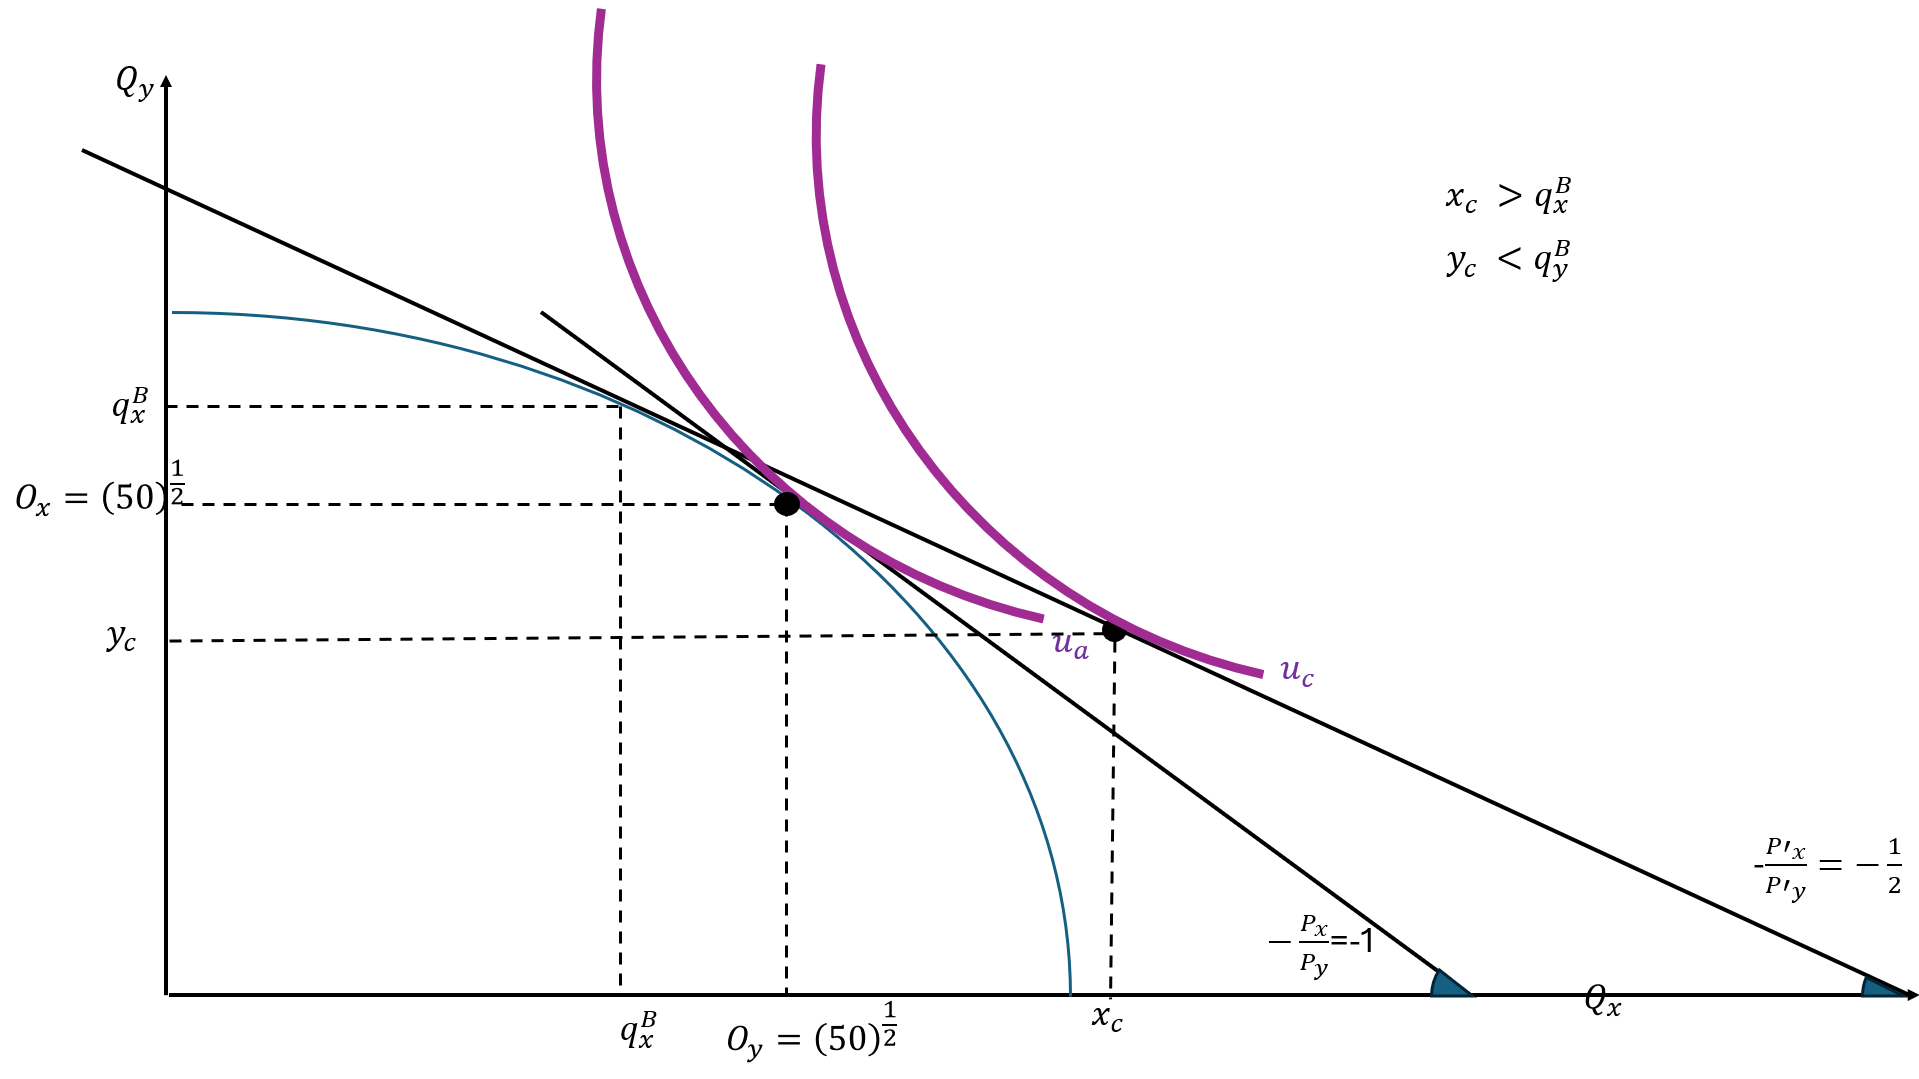
\includegraphics[width=0.7\linewidth]{Imagens/a6i2.png}
\end{figure}

\newpage

\section{\textbf{Modelo Ricardiano}}
\subsection{\textbf{Motivação}}
Um país que seja mais \textbf{produtivo} em todos os bens pode beneficiar-se ao participar do comércio internacional?

A especialização da produção pode trazer ganhos de bem-estar?

Baseado nas ideias do economista clássico David Ricardo (1772-1823)

Por que os países fazem comércio?\begin{itemize}
    \item As diferenças de tecnologias fomentam o comércio entre países 
    \item Explorar diferenças tecnológicas entre eles
    \item Um país produz um dado conjunto de bens de forma mais eficiente que o outro
    \item Poder concentrar esforços produtivos neste conjunto de bens e obter os outros bens de forma mais barata
    \item Especializar-se na produção, mas não no consumo
\end{itemize}

\textbf{Principais insights}\begin{itemize}
    \item Mesmo um país menos eficiente na produção de todos os bens produzirá e exportará algo
    \item O país somente precisa ser relativamente eficiente na produção de um conjunto de bens
    \item Vantagens comparativas vs vantagens absolutas
\end{itemize}

\textbf{Limitações}\begin{itemize}
    \item Mensuração
    \item Distribuição de renda 
\end{itemize}

\subsection{\textbf{Vantagens Absolutas x Vantagens Comparativas}}
\begin{table}[H]
    \centering
    \begin{tabular}{|c|c|c|}
    \hline
    \textbf{}                                                                          & \textit{\textbf{Portugal}} & \textit{\textbf{Inglaterra}} \\ \hline
    \textit{\begin{tabular}[c]{@{}c@{}}Vinho\\ (barril/hora de trabalho)\end{tabular}} & 6                          & 1                            \\ \hline
    \textit{\begin{tabular}[c]{@{}c@{}}Tecido\\ (rolo/hora de trabalho)\end{tabular}}  & 4                          & 2                            \\ \hline
    \end{tabular}
\end{table}
\begin{enumerate}
    \item Qual país apresenta \textbf{vantagem absoluta} na produção de vinhos? Portugal possui a vantagem absoluta na produção de vinhos, pois ele produz mais vinho em uma hora, o mesmo argumento é válido para produção de tecido. Ele é mais produtivo em ambos os bens. \(VA_V=Portugal \ \ , \ \ VA_T=Portugal\)
    \item Calcule o custo de oportunidade do vinho em cada país? Tudo o que eu abro mão para fazer outra coisa. Tenho uma hora de trabalho, eu vou produzir vinhos ou tecidos? \(CO_V^P=\frac{4}{6}=\frac{2}{3}\) rolos por barris. \(CO_V^I=\frac{2}{1}\) rolos por barris na Inglaterra. Olhando o custo de oportunidade de produzir tecido em Portugal \((CO_V^P)^{-1}=CO_T^P=\frac{6}{4}=\frac{3}{2}\) barril por rolo, o mesmo vale para a Inglaterra \((CO_V^I)^{-1}=CO_T^I=\frac{1}{2}\) barril por rolo
    \item Qual país apresenta \textbf{vantagem comparativa} na produção de vinho? Agora temos que olhar o custo de oportunidade, é mais custoso produzir vinho na Inglaterra do que em Portugal(Portugal possui vantagem comparativa na produção de vinho). É mais custoso produzir tecido em Portugal do que na Inglaterra(Inglaterra possui vantagem comparativa na produção de tecido).
    \item Se esses países decidissem se especializar em apenas um dos bens, qual seria o produto mais indicado para cada país? Portugal vai se especializar em produzir vinho e a Inglaterra vai se especializar em produzir tecido. Eles vão produzir aquilo que eles tem vantagem comparativa. 
    \item Qual poderia ser o preço(relativo) do vinho em uma eventual transação comercial entre os dois países?\(\frac{P_V}{P_T}\approx[\frac{2}{3},2]\) o preço relativo do vinho ficou entre os custos de oportunidade dos vinhos entre os países. Do tecido teria a mesma ideia.
\end{enumerate}

\subsubsection{\textbf{Vantagem comparativa}}
É a habilidade de um país de produzir um bem ou serviço a um custo de oportunidade menor do que o seu concorrente\begin{itemize}
    \item Ter vantagem comparativa \textbf{não} significa que o país é melhor na produção desse bem/serviço em termos \textbf{absolutos}
    \item Os países derivam \textbf{ganhos de comércio} a partir da especialização
    \item Vamos discutir um modelo para entender como a vantagem comparativa determina o padrão do comércio internacional
\end{itemize}

\subsection{\textbf{Um Modelo Simples}}
\subsubsection{\textbf{Hipóteses}}
Dois bens: bem 1 e bem 2
\begin{itemize}
    \item Cada um produzido em um setor diferente
\end{itemize}

Dois países: Local e Estrangeiro
\begin{itemize}
    \item Estrangeiro identificado por um asterisco
    \item Inicialmente isolado (sem comércio)
    \item Diferenças tecnológicas entre setores e países
\end{itemize}

Um único fator de produção: trabalho
\begin{itemize}
    \item Perfeita mobilidade entre setores (longo prazo)
    \item Nenhuma mobilidade entre países (não há imigração)
\end{itemize}

Concorrência perfeita; bens homogêneos

Funções de produção (Local)\begin{itemize}
    \item \(Q_1= \underbrace{\frac{1}{a_{L_1}}}_\text{Medida de Produtividade}L_1 \ \ ; \ \ Q_2= \frac{1}{a_{L_2}}L_2\)
    \item \(Q_i\): produção do bem \(i=1,2\)
    \item \(L_i\): quantidade de trabalho contratada pelo setor \(1,2\)
\end{itemize}

Analogamente para estrangeiro:
\[
Q^*_1=\frac{1}{a_{L_1}^*}L_1^* \ \ ; \ \ Q^*_2=\frac{1}{a_{L_2}^*}L_2^*
\]

\subsubsection{\textbf{Tecnologia}}
Parâmetros tecnológicos:\(a_{L_1},a_{L_2},a_{L_1}^*,a_{L_2}^*\)\begin{itemize}
    \item Quantidade de trabalho necessária para produzir 1 unidade de cada bem.
    \item Para produzir 1 unidade do bem 1 no país Local, uma firma precisa contratar \(a_{L_1}\) trabalhadores
    \item É uma medida de ineficiência, quanto maior o valor de \(a_{L_i}\), mais ineficiente é a produção de um bem. 
\end{itemize}

Retornos constantes de escala: para produzir \(Z\) unidades é necessário para contratar \(a_{L_1}Z\) trabalhadores:\begin{itemize}
    \item das funções de produção: \(L_i=a_{L_i}Q_i \ , \ i=1,2\)
\end{itemize}

\textbf{Hipótese principal}: parâmetros tecnológicos diferem entre países

\subsubsection{\textbf{Fronteira de Possibilidades de Produção (FPP)}}

Existem \(\overline{L}\) trabalhadores(dotação de trabalho) no país Local divididos entre setores 1 e 2
\[
L_1+L_2=\overline{L}
\]

Usando as funções de produção, podemos obter a \textbf{FPP} para o país loccal
\[
a_{L_1}Q_1+a_{L_2}Q_2=\overline{L}
\]

Analogamente, a dotação de trabalho do país Estrangeiro é \(\overline{L}^*\) e a \textbf{FPP}
\[
a_{L_1}^*Q_1^*+a_{L_2}^*Q_2^*=\overline{L}^*
\]

Rearranjando a equação para o país Local
\[
Q_2=\frac{\overline{L}}{a_{L_2}}-\frac{a_{L_1}}{a_{L_2}}Q_1
\]

\begin{figure}[H]
    \centering
    \includegraphics[width=0.7\linewidth]{Imagens/a7i4.png}
\end{figure}

Inclinação da \textbf{FPP} do país Local(em valores absolutos)
\[
-\frac{dQ_2}{dQ_1}=\frac{a_{L_1}}{a_{L_2}}=\textbf{TMT}
\]

\textbf{Custo de Oportunidade}\begin{itemize}
    \item Para aumentar a produção do bem 1, a economia precisa produzir menos do bem 2
    \item Trabalhadores precisam ser realocados
\end{itemize}

\begin{figure}[H]
    \centering
    \includegraphics[width=0.7\linewidth]{Imagens/a7i1.png}
\end{figure}

\subsection{\textbf{Produção}}
\subsubsection{\textbf{Concorrência Perfeita}}
\textbf{FPP}: combinações de \( Q_1 \) e \( Q_2 \) que um país \textbf{pode} produzir
\begin{itemize}
    \item \textbf{A produção} efetiva depende dos preços dos bens (\( P_1 \) e \( P_2 \))
\end{itemize}

\textbf{Concorrência perfeita}: firmas em cada setor decidem o quanto produzir e quantos trabalhadores contratar tomando como dados os preços dos bens e os salários (\( w \))

\textbf{Livre mobilidade}: trabalhadores escolhem o setor que paga o maior salário

Portanto, existirá apenas um salário \( w \) para toda a economia
\begin{itemize}
    \item Ambos os setores pagam os mesmos salários, ou
    \item Existe apenas um setor ativo (o outro está fora do mercado)
\end{itemize}

Lucro de uma firma do setor 1 no país Local(repare que o salário é o mesmo para todos os setores)
\[
\pi_1=P_1Q_1-wL_1=P_1\frac{L_1}{a_{L_1}}-wL_1
\]
\[
\pi_1=\left[\frac{P_1}{a_{L_1}}-w\right]L_1
\]
\[
\max_{L_1}\pi_1=\left[\frac{P_1}{a_{L_1}}-w\right]L_1 
\]
Como é um problema linear, as soluções serão de canto, dado que eu preciso derivar duas vezes em relação a \(L_1\) e a segunda derivada deve ser negativa, impossível nesse caso.

A expressão que está dentro dos colchetes\((\frac{P_1}{a_{L_1}}-w)\) não pode ser positiva\begin{itemize}
    \item Do contrário, as firmas poderiam aumentar os lucros indefinidamente contratando mais pessoas
    \item Demanda por trabalho seria infinita; não pode ser um equilíbrio, uma vez que há um número finito de trabalhadores
\end{itemize}

Se negativo\begin{itemize}
    \item \(w>\frac{P_1}{a_{L_1}}\).Logo \(\pi_1<0\) para \(L_1>0\)\begin{itemize}
        \item As firmas não vão produzir: \(Q_1=L_1=0\), esse setor está fechado, ele não produz nesse país.
    \end{itemize}
\end{itemize}

Se igual a zero\begin{itemize}
    \item \(w=\frac{P_1}{a_{L_1}}\).Logo \(\pi_1=0\) para \(L_1\ge0\)\begin{itemize}
        \item Firmas são indiferentes entre qualquer nível de emprego/produção
        \item Portanto, \(Q_1>0\) é o caso em que \(w=\frac{P_1}{a_{L_1}}\)
    \end{itemize}
\end{itemize}

Analogamente para o setor 2\begin{itemize}
    \item Se \(w>\frac{P_2}{a_{L_2}}\), então \(Q_2=L_2=0\)
    \item Se \(w=\frac{P_2}{a_{L_2}}\), então \(Q_2\ge 0\), \(L_2\ge 0\)
\end{itemize}

A situação em vermelho não existe.

\begin{table}[H]
\centering
\begin{tabular}{c|c|c|}
\cline{2-3}
\textbf{}                                                         & \textit{\textbf{\(w>\frac{P_2}{a_{L_2}}\)}}                                                                                         & \textit{\textbf{\(w=\frac{P_2}{a_{L_2}}\)}}                                                                                         \\ \hline
\multicolumn{1}{|c|}{\textit{\textbf{\(w>\frac{P_1}{a_{L_1}}\)}}} & \cellcolor[HTML]{FD6864}\begin{tabular}[c]{@{}c@{}}\(L_1=0 \ \ , \ \  Q_1=0 \)\\ \(L_2=0 \ \ , \ \ Q_2=0 \)\end{tabular}            & \begin{tabular}[c]{@{}c@{}}\(L_1=0 \ \ , \ \ Q_1=0\)\\ \(L_2=\overline{L} \ \ , \ \ Q_2=\frac{\overline{L}}{a_{L_2}}\)\end{tabular} \\ \hline
\multicolumn{1}{|c|}{\textit{\textbf{\(w=\frac{P_1}{a_{L_1}}\)}}} & \begin{tabular}[c]{@{}c@{}}\(L_1=\overline{L} \ \ , \ \ Q_1=\frac{\overline{L}}{a_{L_1}}\)\\ \(L_2=0 \ \ , \ \ Q_2=0\)\end{tabular} & \begin{tabular}[c]{@{}c@{}}\(L_1\ge 0 \ \ , \ \ Q_1 \ge 0\)\\ \(L_2\ge 0\ \  ,\ \ Q_2 \ge 0\)\end{tabular}                          \\ \hline
\end{tabular}
\end{table}


\subsubsection{\textbf{Três Possibilidades}}
\begin{table}[H]
    \centering
\begin{tabular}{c|c|c|}
    \cline{2-3}
    \textbf{}                                                         & \textit{\textbf{\(w>\frac{P_2}{a_{L_2}}\)}}                                                & \textit{\textbf{\(w=\frac{P_2}{a_{L_2}}\)}}                                               \\ \hline
    \multicolumn{1}{|c|}{\textit{\textbf{\(w>\frac{P_1}{a_{L_1}}\)}}} & \begin{tabular}[c]{@{}c@{}}\(Q_1=0 \)\\ \(Q_2=0\)\end{tabular}                             & \begin{tabular}[c]{@{}c@{}}\(Q_1=0\) \\ \(Q_2=\frac{\overline{L}}{a_{L_2}}\)\end{tabular} \\ \hline
    \multicolumn{1}{|c|}{\textit{\textbf{\(w=\frac{P_1}{a_{L_1}}\)}}} & \begin{tabular}[c]{@{}c@{}}\(Q_1=\frac{\overline{L}}{a_{L_1}}\) \\ \(Q_2=0 \)\end{tabular} & \begin{tabular}[c]{@{}c@{}}\(Q_1 \ge 0\)\\ \(Q_2 \ge 0\)\end{tabular}                     \\ \hline
    \end{tabular}
\end{table}

A primeira célula não pode ser um equilíbrio\begin{itemize}
    \item Demanda por trabalho seria igual a zero
\end{itemize}

Ficamos, então, com três possibilidades

Apenas o bem 1 é produzido quando:

\[
w = \frac{P_1}{a_{L_1}} > \frac{P_2}{a_{L_2}} \iff \frac{P_1}{P_2} > \frac{a_{L_1}}{a_{L_2}} \Rightarrow Q_1 = \frac{\bar{L}}{a_{L_1}} \ \ , \ \ \overline{L}=L_1 \ \ , \ \ Q_2 = 0 \ \ , \ \ L_2=0
\]

Apenas o bem 2 é produzido quando:

\[
w = \frac{P_2}{a_{L_2}} > \frac{P_1}{a_{L_1}} \iff \frac{P_1}{P_2} < \frac{a_{L_1}}{a_{L_2}} \Rightarrow Q_1 = 0 \ \ ,\ \ L_1=0 \ \ , \ \  Q_2 = \frac{\bar{L}}{a_{L_2}} \ \ , \ \ \overline{L}=L_2
\]

Ambos os bens são produzidos (potencialmente) quando:

\[
w = \frac{P_1}{a_{L_1}} = \frac{P_2}{a_{L_2}} \iff \frac{P_1}{P_2} = \frac{a_{L_1}}{a_{L_2}} \Rightarrow L_1 \ge 0 \ \ , \ \ Q_1 \geq 0 \ \ , \ \ L_2 \ge 0 \ \ , \ \ Q_2 \geq 0
\] (qualquer ponto na FPP).

\begin{figure}[H]
    \centering
    \includegraphics[width=0.7\linewidth]{Imagens/a7i2.png}
\end{figure}

\subsection{\textbf{Autarquia}}
\subsubsection{\textbf{Demanda}}
\textbf{Vamos assumir algumas hipóteses sobre a demanda}\begin{itemize}
    \item Consumidores gostam tanto do bem 1 quanto do bem 2
    \item Eles possuem curvas de indiferença convexas em direção à origem\begin{itemize}
        \item Preferem combinações balanceadas dos dois bens ao invés de cestas extremas 
    \end{itemize}
    \item Curvas de indiferença não tocam os eixos\begin{itemize}
        \item Utilidade marginal de consumir um dado bem vai ao infinito à medida que o seu consumo se aproxima de zero
    \end{itemize}
    \item \(C_i\): consumo total do bem \(i=1,2\)
\end{itemize}

\begin{figure}[H]
    \centering
    \includegraphics[width=0.7\linewidth]{Imagens/a7i3.png}
\end{figure}

\subsubsection{\textbf{Equilíbrio}}
Portanto, deve ser o caso em que
\[
C_1>0 \ \ , \ \ C_2>0 
\]

Em autarquia (sem comércio), todo o consumo de um país deve ser provido pelas firmas locais
\[
C_1=Q_1
\]
\[
C_2=Q_2
\]

Logo, 
\[Q_1>0 \ \ , \ \ Q_2>0 \]

Produção não pode ocorrer nos cantos da FPP\begin{itemize}
    \item Só é possível se \(\frac{P_1}{P_2}=\frac{a_{L_1}}{a_{L_2}}\)
\end{itemize}

Podemos, então, fixar os preços de equilíbrio em autarquia:\begin{itemize}
    \item \textbf{Local:}
    \[
    \left( \frac{P_1}{P_2} \right)_{\text{aut}} = \frac{a_{L_1}}{a_{L_2}}
    \]

    \item \textbf{Estrangeiro:}
    \[
    \left( \frac{P_1^*}{P_2^*} \right)_{\text{aut}} = \frac{a_{L_1}^*}{a_{L_2}^*}
    \]
\end{itemize}

\subsection{\textbf{Comércio}}
\subsubsection{\textbf{Vantagens Comparativas}}
\textbf{Hipótese principal}\begin{itemize}
    \item Diferenças tecnológicas: \( \frac{a_{L_1}}{a_{L_2}} \neq \frac{a^*_{L_1}}{a^*_{L_2}} \)
    \item Isso dá origem a diferenças de preços em autarquia
    \item Motivação para o comércio
\end{itemize}

Especificamente, o país \textit{Local} possui \textbf{vantagens comparativas} na produção do bem 1.

\textit{Estrangeiro} possui \textbf{vantagens comparativas} na produção do bem 2

\[
\frac{a_{L_1}}{a_{L_2}} < \frac{a^*_{L_1}}{a^*_{L_2}}
\]

Portanto, o bem 1 será relativamente mais barato no país \textit{Local}

\[
\left( \frac{P_1}{P_2} \right)_{\text{aut}} < \left( \frac{P_1^*}{P_2^*} \right)_{\text{aut}}
\]

Quando eles se abrem para o comércio, o país \textit{Local} irá exportar o bem 1 e o país \textit{Estrangeiro} exportará o bem 2.

Cada país exporta o bem em que possui vantagem comparativa.

\subsubsection{\textbf{Vantagens Comparativas vs Vantagens Absolutas}}
Dizemos que o país \textit{Local} tem \textbf{vantagens absolutas} na produção de um bem se 
\( a_{L_i} < a^*_{L_i} \)

\begin{itemize}
    \item \textit{Estrangeiro} tem vantagem absoluta \( \rightarrow a^*_{L_i} < a_{L_i} \)
\end{itemize}

No modelo Ricardiano, vantagem absoluta é irrelevante para determinar a direção dos fluxos de comércio (apenas vantagem comparativa importa).

Em outras palavras, um país pode ser menos eficiente na produção de todos os bens e ainda assim exportar alguma coisa.

\begin{itemize}
    \item Por exemplo, se \( a_{L_1} < a^*_{L_1} \) e \( a_{L_2} < a^*_{L_2} \), mas 
    \(
    \frac{a_{L_1}}{a_{L_2}} < \frac{a^*_{L_1}}{a^*_{L_2}}
    \)
    \item País \textit{Estrangeiro} não tem vantagem absoluta em nenhum dos bens, mas possui vantagem comparativa no bem 2.
    \item Quando os países comercializarem, o \textit{Estrangeiro} exportará o bem 2.
\end{itemize}

\subsubsection{\textbf{Equilíbrio em Economia Aberta}}
Suponha que os países possam trocar livremente um com o outro \begin{itemize}
    \item Por simplicidade, não há barreiras ao comércio
    \item Preços convergem
\end{itemize}

Agora, países podem se especializar \begin{itemize}
    \item Consumo Mundial = Produção Mundial (não em cada país)
\end{itemize}

\[
\mathcal{C}_1 + \mathcal{C}_1^* = Q_1 + Q_1^*
\]

\[
\mathcal{C}_2 + \mathcal{C}_2^* = Q_2 + Q_2^*
\]

Suponha que os países sejam diferentes apenas nos parâmetros tecnológicos e no tamanho \begin{itemize}
    \item Em particular, preferências homogêneas entre os países
    \item Foco em diferenças tecnológicas impulsionando comércio
\end{itemize}

Em uma economia aberta, os preços relativos são determinados pela interação entre a oferta relativa mundial e a demanda relativa.

\textbf{Oferta relativa} \begin{itemize}
    \item Para diferentes preços relativos $P_1/P_2$, quanto o mundo produz do bem 1 relativamente ao bem 2?
\end{itemize}

\textbf{Lembre-se da regra}

\[
\frac{P_1}{P_2} > \frac{a_{L_1}}{a_{L_2}} \Rightarrow Q_1 = \frac{\bar{L}}{a_{L_1}}, \quad Q_2 = 0 \tag{1}
\]

\[
\frac{P_1}{P_2} < \frac{a_{L_1}}{a_{L_2}} \Rightarrow Q_1 = 0, \quad Q_2 = \frac{\bar{L}}{a_{L_2}} \tag{2}
\]

\[
\frac{P_1}{P_2} = \frac{a_{L_1}}{a_{L_2}} \Rightarrow Q_1 \geq 0, \quad Q_2 \geq 0 \tag{3}
\]

\begin{figure}[H]
    \centering
    \includegraphics[width=0.7\linewidth]{Imagens/a8i1.png}
\end{figure}

\begin{figure}[H]
    \centering
    \includegraphics[width=0.7\linewidth]{Imagens/a8i2.png}
\end{figure}

Se \(\frac{P_1}{P_2} < \frac{a_{L_1}}{a_{L_2}} < \frac{a^*_{L_1}}{a^*_{L_2}}\), então (2) vale para ambos os países

\[
Q_1 = Q_1^* = 0, \quad Q_2 = \frac{\bar{L}}{a_{L_2}}, \quad Q_2^* = \frac{\bar{L}}{a^*_{L_2}} 
\]

\[
\frac{Q_1 + Q_1^*}{Q_2 + Q_2^*} = 0
\]

Se \(\frac{a_{L_1}}{a_{L_2}} < \frac{P_1}{P_2} < \frac{a^*_{L_1}}{a^*_{L_2}}\), então (1) vale para \textit{Local} e (2) para \textit{Estrangeiro}

\[
Q_1 = \frac{\bar{L}}{a_{L_1}}, \quad Q_2 = 0, \quad Q_1^* = 0, \quad Q_2^* = \frac{\bar{L}^*}{a^*_{L_2}}
\]

\[
\frac{Q_1 + Q_1^*}{Q_2 + Q_2^*} = \frac{\bar{L} / a_{L_1}}{\bar{L}^* / a^*_{L_2}}
\]

\begin{figure}[H]
    \centering
    \includegraphics[width=0.7\linewidth]{Imagens/a8i3.png}
\end{figure}

Se \(\frac{P_1}{P_2} = \frac{a_{L_1}}{a_{L_2}} < \frac{a^*_{L_1}}{a^*_{L_2}}\): (3) vale para \textit{Local} e (2) para \textit{Estrangeiro} \begin{itemize}
    \item \textbf{Produção do Local em algum ponto ao longo da FPP}
    \[
    Q_1, Q_2 \geq 0, \quad Q_1^* = 0, \quad Q_2^* = \frac{\bar{L}}{a^*_{L_2}}
    \]
\end{itemize}

Se \(\frac{a_{L_1}}{a_{L_2}} < \frac{P_1}{P_2} = \frac{a^*_{L_1}}{a^*_{L_2}}\): (1) vale para \textit{Local} e (3) para \textit{Estrangeiro} \begin{itemize}
    \item \textbf{Produção do Estrangeiro em algum ponto ao longo da FPP}
    \[
    Q_1 = \frac{\bar{L}}{a_{L_1}}, \quad Q_2 = 0, \quad Q_1^*, Q_2^* \geq 0
    \]
\end{itemize}

\begin{figure}[H]
    \centering
    \includegraphics[width=0.7\linewidth]{Imagens/a8i4.png}
\end{figure}

\subsubsection{\textbf{Curva de Demanda Relativa (RD)}}

\textbf{Consumidores possuem preferências homogêneas} \begin{itemize}
    \item Valorizam o consumo de ambos os bens
    \item A utilidade marginal de um bem vai a infinito à medida que o consumo vai para zero
    \item Se \( P_1 / P_2 \) aumenta, consumidores desejam menos do bem 1 relativamente ao bem 2
    \item Foco no comércio vindo de diferenças tecnológicas
\end{itemize}

\textbf{Logo, a curva de demanda relativa} \begin{itemize}
    \item Negativamente inclinada
    \item Não toca os eixos
    \item Igual para \textit{Local} e \textit{Estrangeiro} (e para o mundo)
\end{itemize}

\textbf{Preferências homogêneas e homotéticas}

\begin{figure}[H]
    \centering
    \includegraphics[width=0.7\linewidth]{Imagens/a8i5.png}
\end{figure}

\subsubsection{\textbf{Equilíbrio na Economia Aberta}}
No equilíbrio de economia aberta

\[
\boxed{\textit{Oferta Relativa} = \textit{Demanda Relativa}}
\]

Vamos mostrar um exemplo em que ambos os países se especializam

\[
\left( \frac{P_1}{P_2} \right)_{\textit{aberta}} \quad : \text{preço relativo de equilíbrio}
\]

\begin{figure}[H]
    \centering
    \includegraphics[width=0.7\linewidth]{Imagens/a8i6.png}
\end{figure}

Ambos os países se especializam \begin{itemize}
    \item \textit{Local} no bem 1 e \textit{Estrangeiro} no bem 2
\end{itemize}

Isso é possível em uma economia aberta, pois os consumidores podem obter o outro bem através do comércio.

\textbf{País Local}: exporta o bem 1, importa o bem 2

\textbf{País Estrangeiro}: exporta o bem 2, importa o bem 

\textbf{Resultado Principal}:Cada país exporta o bem em que possui vantagem comparativa

\subsubsection{\textbf{Mudando o Tamanho dos Países}}
Considere uma configuração diferente em que o país Local  é suficientemente grande comparado ao país Estrangeiro.\begin{enumerate}
    \item Determine o novo preço de equilíbrio de livre comércio
    \item O que você pode dizer sobre a eficiência da produção mundial?
    \item Como fica a divisão dos ganhos de comércio entre Local  e Estrangeiro  nesse caso?
\end{enumerate}

\newpage
\section{\textbf{Modelo Ricardiano: Bem Estar}}
\subsection{\textbf{Bem Estar}}
\subsubsection{\textbf{Efeitos sobre Salários}}
Para avaliar os efeitos do comércio sobre bem-estar, precisamos olhar apenas para os salários.\begin{itemize}
    \item Há um único fator de produção: trabalho. 
    \item Não há muito o que dizer sobre efeitos distributivos. Lembrando que nesse modelo, devido a está suposição, não há como ver efeitos de ganhadores e perdedores, por exemplo, se o salário de um trabalhador sobe, o de todos sobem.
\end{itemize}

Salário real: poder de compra dos salários, assim vamos saber quantos bens o indivíduo consegue comprar antes e depois do comércio. Mas para usar o salário real, temos que saber como funciona seu consumo, não supomos as preferências dos consumidores.

Não fizemos hipóteses específicas sobre a demanda.

Mas para usar o salário real, temos que saber como funciona seu consumo, não supomos as preferências dos consumidores.Portanto, vamos olhar para dois casos extremos.\begin{itemize}
    \item Consumidores se preocupam apenas com o bem 1: \( \frac{w}{P_1} \).
    \item Consumidores se preocupam apenas com o bem 2: \( \frac{w}{P_2} \).
    \item Impacto sobre os salários reais em algum lugar no meio.
    \item O mundo vai ser uma "média" desses dois extremos. 
\end{itemize}

Foco no caso em que ambos os países se especializam.

\begin{itemize}
    \item \textit{Local} se especializa no bem 1.
    \item \textit{Estrangeiro} se especializa no bem 2.
\end{itemize}

Em comparação com os preços relativos de autarquia (ver Figura):\begin{itemize}
    \item Comércio faz preços relativos aumentarem no país \textit{Local}.
    \item E caírem no país \textit{Estrangeiro}.
\end{itemize}

\[
\frac{a_{L_1}}{a_{L_2}} = \frac{P_1}{P_2} < \frac{P_1'}{P_2'} < \frac{P_1^*}{P_2^*} = \frac{a_{L_1}^*}{a_{L_2}^*}
\]

\begin{itemize}
    \item Linha = preços de economia aberta (igual para os países).
    \item Sem linha = preços de autarquia.
\end{itemize}

\begin{figure}[H]
    \centering
    \includegraphics[width=0.7\linewidth]{Imagens/a9i1.png}
\end{figure}

Lembre-se de que, em autarquia, os países precisam produzir ambos os bens:

\[
w = \frac{P_1}{a_{L_1}} = \frac{P_2}{a_{L_2}} \quad \text{e} \quad w^* = \frac{P_1^*}{a_{L_1}^*} = \frac{P_2^*}{a_{L_2}^*}
\]

Preços de autarquia em termos dos bens 1 e 2 são:

\textit{Local}:
\[
\frac{w}{P_1} = \frac{1}{a_{L_1}}; \quad \frac{w}{P_2} = \frac{1}{a_{L_2}}
\]

\textit{Estrangeiro}:
\[
\frac{w^*}{P_1^*} = \frac{1}{a_{L_1}^*}; \quad \frac{w^*}{P_2^*} = \frac{1}{a_{L_2}^*}
\]

Dado que os países se especializam em uma economia aberta:

\[
w' = \frac{P_1'}{a_{L_1}} > \frac{P_2'}{a_{L_2}} 
\quad \text{e} \quad 
w^{*'} = \frac{P_2^{*'}}{a_{L_2}^*} > \frac{P_1^{*'}}{a_{L_1}^*}
\]

Em termos reais:

\[
\underbrace{\frac{w'}{P_1'} = \frac{1}{a_{L_1}} = \frac{w}{P_1} : \text{Inalterado}}_\text{País Local e Bem 1}
\quad \text{e} \quad 
\underbrace{\frac{w^{*'}}{P_2^{*'}} = \frac{1}{a_{L_2}^*} = \frac{w^*}{P_2^*} : \text{Inalterado}}_\text{País Estrangeiro e Bem 2}
\]

Portanto, em termos do bem exportado, os salários não mudam.

Salários aumentam em termos do bem importado(bem 2) no país \textit{Local}

\[
\frac{w'}{P_2'} = \underbrace{\frac{P_1'}{P_2'}}_\text{Preço de Livre Comércio} \frac{1}{a_{L_1}} > \underbrace{\frac{a_{L_1}}{a_{L_2}}}_\text{Custo Relativo de Produzir o Bem 1} \frac{1}{a_{L_1}} = \frac{1}{a_{L_2}} = \frac{w}{P_2}
\]


Os salários no país \textit{Local}
\begin{itemize}
    \item São constantes em termos do bem 1 (exportado)
    \item Aumentam em termos do bem 2 (importado)o poder de compra em temos das importações aumentam.
\end{itemize}

Portanto, os salários reais aumentam.

Analogamente, para o país \textit{Estrangeiro}

\[
\frac{w^{*'}}{P_1'} = \frac{P_2'}{P_1'} \frac{1}{a_{L_2}^*}
\]

Dado que 
\[
\frac{P_1'}{P_2'} < \frac{P_1^*}{P_2^*} = \frac{a_{L_1}^*}{a_{L_2}^*}
\]
então 
\[
\frac{P_2'}{P_1'} > \frac{a_{L_2}^*}{a_{L_1}^*}
\]
Portanto,

\[
\frac{w^{*'}}{P_1'} = \underbrace{\frac{P_2'}{P_1'}}_\text{Preço de Livre Comércio} \frac{1}{a_{L_2}^*} > \underbrace{\frac{a_{L_2}^*}{a_{L_1}^*}}_\text{Custo Relativo de Produzir o Bem 2} \frac{1}{a_{L_2}^*} = \frac{1}{a_{L_1}^*} = \frac{w^*}{P_1^*}
\]

Os salários no país \textit{Estrangeiro}:
\begin{itemize}
    \item Constantes em termos do bem 2 (exportado)
    \item Aumentam em termos do bem 1 (importado)
\end{itemize}

Portanto, os salários reais aumentam.

Salários reais aumentam em ambos os países.

Ambos os países ganham com o comércio:
\begin{itemize}
    \item Ganhos são distribuídos igualmente - há apenas trabalho
    \item Não há perdedores
\end{itemize}

Você deve verificar o caso de países grandes/pequenos:
\begin{itemize}
    \item Se um país for suficientemente grande, então ele não ganhará nada com o comércio
\end{itemize}

Vamos revisitar esses resultados:
\begin{itemize}
    \item Mais estrutura do lado da demanda
    \item Primeiro, uma revisão de micro
\end{itemize}


\subsection{\textbf{Revisão}}
\subsubsection{\textbf{Curvas de Indiferença Comunitárias}}

Referência: Markussen et al., cap. 3 \href{https://mpra.ub.uni-muenchen.de/21989/1/MPRA_paper_21989.pdf}{[Link]}

Lado da demanda: consumidores/trabalhadores obtêm renda do trabalho; renda usada para comprar bens 1 e 2.

Existem \( j = 1,2, \cdots , N \) consumidores em um país (por ex., \textit{Local}).

Consumidor \( j \) gosta de ambos os bens; preferências podem ser representadas pela seguinte função utilidade:\begin{itemize}
    \item \[
            U_j(c_{1j}, c_{2j})
          \]
    \item Crescente em ambos os argumentos.
    \item Curvas de indiferença convexas em relação à origem e nunca tocam os eixos.
\end{itemize}

\begin{figure}[H]
    \centering
    \includegraphics[width=0.7\linewidth]{Imagens/a9i2.png}
\end{figure}

Consumidor \( j \) possui renda \( l_j \) e enfrenta preços \( P_1 \) e \( P_2 \).

\begin{itemize}
    \item Possui, portanto, a seguinte restrição orçamentária:
\end{itemize}

\[
P_1 c_{1j} + P_2 c_{2j} = l_j
\]

Reescrevendo:

\[
c_{2j} = \frac{l_j}{P_2} - \frac{P_1}{P_2} c_{1j}
\]

Inclinação da restrição orçamentária (em valores absolutos):

\[
- \frac{dc_{2j}}{dc_{1j}} = \frac{P_1}{P_2}
\]

\begin{figure}[H]
    \centering
    \includegraphics[width=0.7\linewidth]{Imagens/a9i3.png}
\end{figure}

Consumidor escolhe \( c_{1j} \) e \( c_{2j} \) que maximizam a utilidade dados os preços e a renda:

\[
\max U_j(c_{1j}, c_{2j}) \quad \text{s.a.} \quad P_1 c_{1j} + P_2 c_{2j} = l_j
\]

A solução é dada pela condição usual de tangência (próximo slide).

Funções demandas individuais:

\[
c_{1j} = c_{1j}(P_1, P_2, l_j)
\]

\[
c_{2j} = c_{2j}(P_1, P_2, l_j)
\]

\begin{figure}[H]
    \centering
    \includegraphics[width=0.7\linewidth]{Imagens/a9i4.png}
\end{figure}

As demandas totais são dadas por:

\[
C_1 = \sum_{j=1}^{N} c_{1j}(P_1, P_2, l_j)
\]

\[
C_2 = \sum_{j=1}^{N} c_{2j}(P_1, P_2, l_j)
\]

Em princípio, as demandas totais podem depender da distribuição de renda:

\[
C_1 = C_1(P_1, P_2, l_1, l_2, \cdots , l_N)
\]

\[
C_2 = C_2(P_1, P_2, l_1, l_2, \cdots , l_N)
\]

\textbf{Caso especial}  

Se todos os consumidores tiverem a mesma preferência e elas forem \textbf{homotéticas}, as demandas totais dependerão apenas dos preços e da renda total.

\textbf{Preferências homotéticas}: razão \( C_1 / C_2 \) depende apenas dos preços e não da renda.

\[
C_1 = C_1(P_1, P_2, l)
\]

\[
C_2 = C_2(P_1, P_2, l)
\]

onde \( l = \sum_{j=1}^{N} l_j \) é a renda total da economia.

No agregado, a economia é igual ao problema de uma única pessoa que possui renda \( l \):

\begin{itemize}
    \item Bem-estar total é dado pela altura da curva de indiferença dessa pessoa.
    \item \textbf{Curvas de indiferença comunitárias}
\end{itemize}

\begin{figure}[H]
    \centering
    \includegraphics[width=0.7\linewidth]{Imagens/a9i5.png}
\end{figure}

\subsection{\textbf{Bem-Estar}}
\subsubsection{\textbf{De volta ao Modelo Ricardiano}}
Inicialmente, vamos focar no caso em que ambos os países se especializam:

\begin{itemize}
    \item Preferências homogêneas e homotéticas (use curvas de indiferença comunitárias).
    \item Renda total (\textit{Local}) \( l = w \bar{L} \).
\end{itemize}

\textbf{Restrição orçamentária agregada (\textit{Local})}

\[
P_1 C_1 + P_2 C_2 = l
\]

\[
\text{inclinação} = -\frac{dC_2}{dC_1} = \frac{P_1}{P_2}
\]

\begin{figure}[H]
    \centering
    \includegraphics[width=0.7\linewidth]{Imagens/a9i6.png}
\end{figure}

\begin{figure}[H]
    \centering
    \includegraphics[width=0.7\linewidth]{Imagens/a9i7.png}
\end{figure}

Em autarquia, inclinação da restrição orçamentária do país \textit{Local} é:

\[
- \frac{dC_2}{dC_1} = \left(\frac{P_1}{P_2} \right)_{\text{aut}} = \frac{a_{L_1}}{a_{L_2}}
\]

\begin{itemize}
    \item Que é a mesma inclinação da FPP do país \textit{Local}.
\end{itemize}

Portanto, em autarquia, a FPP e a restrição orçamentária agregada coincidem.

Bem-estar é dado pela altura da curva de indiferença comunitária que é tangente a ambas as linhas.

\begin{figure}[H]
    \centering
    \includegraphics[width=0.7\linewidth]{Imagens/a9i8.png}
\end{figure}

\subsubsection{\textbf{Economia Aberta}}
Quando o país \textit{Local} se abre ao comércio, o preço relativo do bem 1 \textbf{aumenta}:

\[
\left( \frac{P_1}{P_2} \right)_{\text{open}} > \left( \frac{P_1}{P_2} \right)_{\text{aut}} = \frac{a_{L_1}}{a_{L_2}}
\]

A restrição orçamentária se torna \textbf{mais inclinada} para o país \textit{Local}:

\begin{itemize}
    \item Ela precisa cruzar o ponto de produção (valor da produção = valor da renda).
\end{itemize}

Comércio permite que o consumo aconteça fora da FPP:

\begin{itemize}
    \item Os pontos de produção e consumo não são mais os mesmos.
\end{itemize}

\begin{figure}[H]
    \centering
    \includegraphics[width=0.7\linewidth]{Imagens/a9i9.png}
\end{figure}

Para o país \textit{Estrangeiro}, o preço relativo do bem 1 \textbf{diminui}:

\[
\left( \frac{P_1}{P_2} \right)_{\text{open}} < \left( \frac{P_1^*}{P_2^*} \right)_{\text{aut}} = \frac{a_{L_1}^*}{a_{L_2}^*}
\]

Restrição orçamentária se torna \textbf{menos inclinada}.

\begin{figure}[H]
    \centering
    \includegraphics[width=0.7\linewidth]{Imagens/a9i10.png}
\end{figure}

\begin{figure}[H]
    \centering
    \includegraphics[width=0.7\linewidth]{Imagens/a9i11.png}
\end{figure}

Ganho de comércio depende do quanto os preços mudam em relação à autarquia.

Veja o exemplo do país \textit{Local} no próximo slide (você pode checar para o \textit{Estrangeiro}).

Diferenças tecnológicas maiores entre os países levam a maiores ganhos de comércio.

\begin{figure}[H]
    \centering
    \includegraphics[width=0.7\linewidth]{Imagens/a9i12.png}
\end{figure}

Considere duas situações com relação às diferenças tecnológicas:

\begin{itemize}
    \item \textbf{Países similares}: \( a_{L_1}/a_{L_2} \) próximo a \( a_{L_1}^*/a_{L_2}^* \).
    \item \textbf{Países bem diferentes}: \( a_{L_1}/a_{L_2} \) muito menor que \( a_{L_1}^*/a_{L_2}^* \).
\end{itemize}

\begin{figure}[H]
    \centering
    \includegraphics[width=0.7\linewidth]{Imagens/a9i13.png}
\end{figure}

Tamanho dos países também pode afetar como os preços relativos mudam:

\begin{itemize}
    \item Países pequenos possuem variação maior nos preços relativos comparado ao nível de autarquia; tendem a se beneficiar mais do comércio.
    \item Países maiores possuem variação menor nos preços relativos comparado ao nível de autarquia.
\end{itemize}

Se um país for suficientemente grande, então seu preço relativo não vai se alterar:

\begin{itemize}
    \item Terá que produzir ambos os bens.
    \item Não há ganho de bem-estar para países grandes.
\end{itemize}

\begin{figure}[H]
    \centering
    \includegraphics[width=0.7\linewidth]{Imagens/a9i14.png}
\end{figure}

\begin{figure}[H]
    \centering
    \includegraphics[width=0.7\linewidth]{Imagens/a9i15.png}
\end{figure}

\begin{figure}[H]
    \centering
    \includegraphics[width=0.7\linewidth]{Imagens/a9i16.png}
\end{figure}

\newpage
\section{\textbf{Modelo de Heckscher-Ohlin: Teorema de Stolper-Samuelson}}
\subsection{\textbf{Motivação}}
\textbf{Por  que  os  países  fazem  Comércio?}\begin{itemize}
    \item Diferenças na dotação de fatores: mão de obra, capital, terra, recursos naturais, etc.
    \item Fatores não podem ser comercializados
    \item Bens funcionam como instrumentos para exportar/importar serviços de fatores
\end{itemize}

\textbf{Mecanismos}\begin{itemize}
    \item Um país tem abundância de um determinado fator (ex: mão de obra) \(\rightarrow\) os salários serão mais baixos neste país
    \item Assim, é possível que bens intensivos em mão de obra sejam produzidos de forma mais barata neste país
    \item Por outro lado, outros fatores (ex: capital) são escassos e caros \(\rightarrow\) produzir bens intensivos em capital é mais custoso
\end{itemize}

\textbf{Portanto,  há  motivação  para  o  Comércio}\begin{itemize}
    \item A abundância de fatores de produção determinará quais bens serão exportados
    \item Um país com uma oferta relativamente alta de mão de obra exportará bens intensivos em trabalho
    \item De forma análoga, países com uma abundância relativa de capital exportarão bens intensivos neste fator
\end{itemize}

\textbf{O  Comércio  traz  uma  transformação  estrutural}\begin{itemize}
    \item No país abundante em mão de obra, o setor trabalho intensivo se expande, enquanto o de bens de capital se contrai
    \item A demanda por trabalho e os salários aumentam
    \item A demanda por capital e a remuneração deste fator diminuem 
\end{itemize}

\textbf{Implicações  para  a  distribuição  de  renda}

\subsection{\textbf{Hipóteses}}
Dois Bens: bem 1 e bem 2   \begin{itemize}
    \item Produzidos em setores separados
\end{itemize}

Dois Países: Local e Estrangeiro\begin{itemize}
    \item Estrangeiro identificado por asterisco
    \item \textbf{Não} há diferença tecnológica entre setores-países
\end{itemize}

Dois fatores de produção: capital (\(K\)) e trabalho (\(L\))\begin{itemize}
    \item Ambos os fatores são móveis entre setores (longo prazo)
    \item Imóveis entre países
\end{itemize}

Competição Perfeita

Países são diferentes na dotação de capital (\(K\)) e trabalho (\(L\))

Idênticos em todas as outras dimensões\begin{itemize}
    \item Tecnologias
    \item Preferências
    \item Comércio motivado por diferenças na dotação de fatores
\end{itemize}

Comparado ao Modelo Ricardiano\begin{itemize}
    \item Dois fatores de produção \(\rightarrow\) distribuição de renda
    \item Tecnologias neste caso são idênticas
\end{itemize}

Ainda são mantidas as hipóteses de competição perfeita, bens homogêneos e retornos constantes de escala

\subsection{\textbf{Tecnologia}}
Países são diferentes na dotação de capital (\(K\)) e trabalho (\(L\))

Idênticos em todas as outras dimensões
\begin{itemize}
    \item Tecnologias
    \item Preferências
    \item Comércio motivado por diferenças na dotação de fatores
\end{itemize}

Comparado ao Modelo Ricardiano
\begin{itemize}
    \item Dois fatores de produção \(\rightarrow\) distribuição de renda
    \item Tecnologias neste caso são idênticas
\end{itemize}

Ainda são mantidas as hipóteses de competição perfeita, bens homogêneos e retornos constantes de escala.

\textbf{Funções de produção apresentam retornos constantes de escala}

\begin{itemize}
    \item Se multiplicarmos todos os insumos por um fator \(\lambda > 0\), então o produto também é multiplicado por \(\lambda\)
    \[
    \lambda Q_i = F_i(\lambda K_i, \lambda L_i) \quad \text{para todo } \lambda > 0, \quad i = 1,2
    \]
\end{itemize}

\textbf{Produtos Marginais}
\[
PMg_{L_i} = \frac{\partial F_i(K_i, L_i)}{\partial L_i}
\]
\[
PMg_{K_i} = \frac{\partial F_i(K_i, L_i)}{\partial K_i}
\]

Produtos marginais são positivos e decrescentes\begin{itemize}
    \item Aumento na quantidade de um insumo mantendo o outro constante
    \item O produto cresce, mas a taxas decrescentes
\end{itemize}

Em termos de derivadas parciais:
\[
\frac{\partial F_i}{\partial L_i} > 0 \quad ; \quad \frac{\partial F_i}{\partial K_i} > 0
\]
\[
\frac{\partial^2 F_i}{\partial L_i^2} < 0 \quad ; \quad \frac{\partial^2 F_i}{\partial K_i^2} < 0
\]

\textbf{Hipótese chave 1}: diferenças tecnológicas entre setores\begin{itemize}
    \item  Setor 1 é \textbf{intensivo em trabalho}
    \item  Setor 2 é \textbf{intensivo em capital}
\end{itemize}

As funções \(F_1\) e \(F_2\) são tais que o setor 1 emprega \textbf{relativamente} mais trabalho que o setor 2

Sob estas condições, podemos definir as seguintes relações capital-trabalho:

\[
k_1 = \frac{K_1}{L_1} \quad ; \quad k_2 = \frac{K_2}{L_2}
\]

Hipótese implica: \( k_1 < k_2 \)


\subsection{\textbf{Retomando as Hipóteses}}
\textbf{Competição Perfeita:} firmas dos dois setores tomam como dados\begin{itemize}
    \item Preços dos bens: \( P_1, P_2 \)
    \item Preços de insumos: salários (\( w \)) e remuneração do capital (\( r \))
\end{itemize}

\textbf{Bens são comercializados entre os países:} comércio afeta preços \(\rightarrow\) preços dos insumos se alteram \(\rightarrow\) muda a distribuição de renda

\textbf{Perfeita mobilidade}\begin{itemize}
    \item Capital e trabalho são móveis entre setores (não entre países)
    \item Para um dado país, salários e remuneração de capital se equalizam
\end{itemize}

\subsection{\textbf{Dotação de Fatores de Produção}}
Dotações de capital e trabalho\begin{itemize}
    \item País Local: \( \bar{K} \) e \( \bar{L} \)
    \item País Estrangeiro: \( \bar{K}^* \) e \( \bar{L}^* \)
\end{itemize}

Equilíbrio no mercado de fatores no país Local

\[
L_1 + L_2 = \bar{L}
\]

\[
K_1 + K_2 = \bar{K}
\]

Analogamente, para o Estrangeiro

\[
L_1^* + L_2^* = \bar{L}^*
\]

\[
K_1^* + K_2^* = \bar{K}^*
\]

\textbf{Hipótese chave 2}: países possuem dotações diferentes dos fatores de produção

\begin{itemize}
    \item Local é \textbf{abundante em capital} (\textit{escasso em trabalho})
    \item Estrangeiro é \textbf{abundante em trabalho} (\textit{escasso em capital})
\end{itemize}

\[
\frac{\bar{K}}{\bar{L}} > \frac{\bar{K}^*}{\bar{L}^*}
\]

\subsection{\textbf{Revisão Micro : Teoria da Produção}}
Agora que há 2 fatores de produção, as firmas devem escolher a combinação de capital e trabalho que irão utilizar
\begin{itemize}
    \item Um dado nível de produção \( Q_i \) pode ser obtido com diferentes combinações de \( K \) e \( L \)
    \item As firmas escolherão a combinação de insumos de menor custo
\end{itemize}

\subsubsection{\textbf{Isoquanta}}
\textbf{Isoquanta}: combinações de capital e trabalho que geram o mesmo nível de produto. Para o setor \( i = 1,2 \)

\[
F_i(K_i, L_i) = \bar{Q}_i
\]

Como as produtividades marginais \( PMg_L \) e \( PMg_K \) são decrescentes, as isoquantas são convexas em relação à origem.

\begin{figure}[H]
    \centering
    \includegraphics[width=0.7\linewidth]{Imagens/a10i1.png}
\end{figure}

\subsubsection{\textbf{Isocusto}}

Combinações de capital e trabalho com o mesmo custo

\[
wL_i + rK_i = C_i
\]

Rearranjando

\[
K_i = \frac{C_i}{r} - \frac{w}{r} L_i
\]

Inclinação

\[
-\frac{dK_i}{dL_i} = \frac{w}{r}
\]

\begin{figure}[H]
    \centering
    \includegraphics[width=0.7\linewidth]{Imagens/a10i2.png}
\end{figure}

\subsubsection{\textbf{Minimização de Custos}}

Qual a combinação de capital e trabalho gera um determinado nível de produto \(\bar{Q}_i\) com o menor custo?

Assuma como dada a isoquanta \(\bar{Q}_i\)

Encontre o ponto associado à menor isoquanta

\[
\min_{L_i,K_i} C_i = wL_i + rK_i \quad \text{s.a.} \quad F_i(K_i, L_i) = \bar{Q}_i
\]


\begin{figure}[H]
    \centering
    \includegraphics[width=0.5\linewidth]{Imagens/a10i3.png}
\end{figure}

\subsubsection{\textbf{Retornos Constantes de Escala}}

Dados \(w , r\), a razão capital-trabalho não depende do nível de produção

Dessa forma é possível resolver o problema para um dado nível \(Q_i\)e escalá-lo para níveis maiores ou menores de produção

\begin{figure}[H]
    \centering
    \includegraphics[width=0.7\linewidth]{Imagens/a10i4.png}
\end{figure}

Assuma que \( a_{K_i} \) e \( a_{L_i} \) sejam a solução do problema para \( Q_i = 1 \)

Para identificar as quantidades de trabalho e capital associadas a diferentes níveis de \( Q_i \), basta multiplicar da maneira apropriada

\[
L_i = a_{L_i} Q_i \quad ; \quad K_i = a_{K_i} Q_i
\]

Razão capital-trabalho: \( k_i = \frac{a_{K_i}}{a_{L_i}} \)

\begin{figure}[H]
    \centering
    \includegraphics[width=0.7\linewidth]{Imagens/a10i5.png}
\end{figure}

Mudanças em \(w/r\) afetam a estratégia de produção das firmas

\begin{figure}[H]
    \centering
    \includegraphics[width=0.7\linewidth]{Imagens/a10i6.png}
\end{figure}

Nesse caso, a empresa está ficando mais capital intensiva, dado o aumento da razão de preços.

\subsection{\textbf{Dois Setores}}
\textbf{Agora podemos expressar os dois setores no mesmo diagrama}\begin{itemize}
    \item Setor 1 é intensivo em trabalho (baixa razão capital-trabalho)
    \item Isoquantas do setor 1 mais próximas do canto inferior direito
    \item Isoquantas do setor 2 mais próximas do canto superior esquerdo
    \item Dado que trabalho e capital são móveis entre setores, \(w\) e \(r\) são equalizados\begin{itemize}
        \item As isocustos dos dois setores são paralelas
    \end{itemize}
\end{itemize}

\begin{figure}[H]
    \centering
    \includegraphics[width=0.7\linewidth]{Imagens/a10i7.png}
\end{figure}

Vamos tornar os setores comparáveis

\begin{itemize}
    \item Nível de produção associado a \$1 em ambos os setores
    \item Permite incorporar os preços dos bens na análise \(\rightarrow\) os quais podem ser afetados pelo Comércio
    \item Inicialmente assumimos que os preços são dados (\textit{``pequena economia aberta''})
    \item Isoquantas de Valor Unitário (setor 1)
\end{itemize}

\[
P_1 Q_1 = 1 \rightarrow P_1 F_1(K_1, L_1) = 1 \Rightarrow F_1(K_1, L_1) = \frac{1}{P_1}
\]

Analogamente, para o setor 2

\[
F_2(K_2, L_2) = \frac{1}{P_2}
\]

Isoquantas agora estão na mesma altura

Vamos supor que ambos os bens são produzidos

\textbf{Importante:} As isoquantas normalizadas em valores unitários não mostram o nível de produção

\subsubsection{\textbf{Isoquantas de Valor Unitário}}
\begin{figure}[H]
    \centering
    \includegraphics[width=0.7\linewidth]{Imagens/a10i8.png}
\end{figure}

Para certas escolhas de insumos, as curvas de isocusto serão as mesmas em ambos os setores

Retornos Constantes de Escala + Competição Perfeita = Lucro Zero

\[
P_1 Q_1 = wL_1 + rK_1 = 1
\]
\[
P_2 Q_2 = wL_2 + rK_2 = 1
\]

Nesse cenário, se ambos os bens são produzidos \(\rightarrow\) \textbf{a mesma isocusto} passa por ambas as isoquantas

Isso nos permite determinar os preços dos fatores \(w\) e \(r\) (nos interceptos)

\begin{itemize}
    \item E também encontrar as razões capital-trabalho
\end{itemize}

\subsubsection{\textbf{Diagrama de Lerner}}
\begin{figure}[H]
    \centering
    \includegraphics[width=0.7\linewidth]{Imagens/a10i9.png}
\end{figure}

\subsection{\textbf{Teorema de Stolper-Samuelson}}
\subsubsection{\textbf{Mudanças nos preços dos bens}}
Podemos usar esse framework para entender como mudanças nos preços dos bens afetam os preços dos fatores\begin{itemize}
    \item E, portanto, a distribuição de renda
\end{itemize}

Política comercial pode influenciar os preços dos bens (mais detalhes depois)\begin{itemize}
    \item Liberalização tende a aumentar o preço do bem exportado
    \item Aumento da proteção eleva o preço do bem importado
\end{itemize}

Considere um aumento em \( P_1 \)\begin{itemize}
    \item No diagrama de Lerner isso leva a um deslocamento para baixo da isoquanta de valor unitário do setor 1
    \item É necessário um número menor de trabalho e capital para gerar o equivalente a \$1
\end{itemize}

\begin{figure}[H]
    \centering
    \includegraphics[width=0.7\linewidth]{Imagens/a10i10.png}
\end{figure}

Um aumento no preço do bem 1 (intensivo em trabalho) gera\begin{itemize}
    \item Aumento nos salários \((1/w\) diminui no diagrama)
    \item Redução na taxa de aluguel \((1/r\) aumenta no diagrama)
\end{itemize}

Dado que o trabalho se torna relativamente mais caro, as firmas de ambos os setores usam \textbf{relativamente} mais capital\begin{itemize}
    \item Como resultado, as razões capital-trabalho aumentam em ambos os setores
\end{itemize}

\subsubsection{\textbf{Mecanismo}}
Aumento de preço incentiva as firmas no setor 1 a expandir a produção\begin{itemize}
    \item Precisam de capital e trabalho, porém, relativamente mais trabalho (tecnologia intensiva em trabalho)
    \item Estes fatores vêm do setor 2 (que está encolhendo)
\end{itemize}

As firmas do setor 1 demandam relativamente mais trabalho, mas o setor 2 libera relativamente mais capital\begin{itemize}
    \item Aos preços iniciais, há excesso de demanda por trabalho e excesso de oferta por capital
    \item Portanto, o salário aumenta e o preço do capital diminui
\end{itemize}

\textbf{Resultado:} expansão do setor 1, contração do setor 2, salários maiores e taxas de aluguel mais baixas

Vamos agora analisar os efeitos de um aumento no preço do bem 2
\begin{figure}[H]
    \centering
    \includegraphics[width=0.7\linewidth]{Imagens/a10i11.png}
\end{figure}

Um aumento no preço do bem 2 (intensivo em capital) gera\begin{itemize}
    \item Redução nos salários (\(1/w\) aumenta no diagrama)
    \item Aumento na taxa de aluguel (\(1/r\) diminui no diagrama)
\end{itemize}

Dado que o capital se torna relativamente mais caro, as firmas de ambos os setores usam \textbf{relativamente} mais trabalho\begin{itemize}
    \item Dado que o capital se torna relativamente mais caro, as firmas de ambos os setores usam \textbf{relativamente} mais trabalho
    \item Como resultado, as razões capital-trabalho diminuem em ambos os setores
\end{itemize}

Aumento de preço incentiva as firmas no setor 2 a expandir a produção\begin{itemize}
    \item Precisam de capital e trabalho, porém, relativamente mais capital (tecnologia intensiva em capital)
    \item Estes fatores vêm do setor 1 (que está encolhendo)
\end{itemize}

As firmas do setor 2 demandam relativamente mais capital, mas o setor 1 libera relativamente mais trabalho\begin{itemize}
    \item Aos preços iniciais, há excesso de demanda por capital e excesso de oferta por trabalho
    \item Portanto, o salário diminui e o preço do capital aumenta
\end{itemize}

\textbf{Resultado:} expansão do setor 2, contração do setor 1, salários menores e taxas de aluguel mais altas.

\subsubsection{\textbf{Resumo}}
\textbf{RESULTADO PRINCIPAL}: \textit{Um aumento no preço de um bem aumenta a remuneração do fator usado intensivamente na produção desse bem e reduz a remuneração do outro fator}

\subsubsection{\textbf{Comentários}}
Efeitos reais sobre os preços dos fatores
\begin{itemize}
    \item Se \(P_1\) sobe, \(w\) aumenta mais do que proporcionalmente
    \item Se \(P_2\) sobe, \(r\) aumenta mais do que proporcionalmente
\end{itemize}

Considere o caso em que \(P_1\) aumenta (\(P_2\) constante)
\begin{itemize}
    \item No diagrama, a linha amarela mostra o quanto a isoquanta de valor unitário se deslocou, i.e., redução de \(1/P_1\)
    \item Note que a redução em \(1/w\) é maior que a queda em \(1/P_1\): \( |\Delta(1/w)| > |\Delta(1/P_1)| \)
    \item Logo, o aumento em \(w\) é maior que o aumento em \(P_1\)
    \item \(w/P_1\) e \(w/P_2\) aumentam; salário real sobe
    \item \(r/P_1\) e \(r/P_2\) diminuem; taxa de aluguel real diminui
\end{itemize}

\begin{figure}[H]
    \centering
    \includegraphics[width=0.7\linewidth]{Imagens/a10i12.png}
\end{figure}

Analogamente para o caso em que \(P_2\) aumento (\(P_1\) constante)\begin{itemize}
    \item No diagrama, você pode verificar que \(|\Delta(1/r)|>|\Delta(1/P_2)|\)
    \item Logo, o aumento em \(r\) é maior que o aumento em \(P_2\)
    \item \(r/P_1\) e \(r/P_2\) aumentam; taxa de aluguel real sobe
    \item \(w/P_1\) e \(w/P_2\) diminuem; salário real dimuniu
\end{itemize}

Efeitos distributivos: alguns fatores podem ser distribuídos de maneira desigual entre os agentes\begin{itemize}
    \item Capital vs Trabalho 
    \item Isto cria um link entre comércio e distribuição de renda
\end{itemize}

Como as razões capital-trabalho nos dois setores aumentam se as dotações de fatores são constantes?\begin{itemize}
    \item Por ex.: quando \(P_1\) aumenta \(\rightarrow k_1 \ e \ k_2 \) sobem 
    \item Com salários relativos mais altos, firmas usam relativamente mais capital em ambos os setores 
    \item Mas as quantidades de capital e trabalho permanecem constantes 
\end{itemize}

Isto pode acontecer porque o tamanho dos setores está mudando\begin{itemize}
    \item Setor trabalho-intensivo se expande
    \item Setor capital-intensivo se contrai
\end{itemize}

Equilíbrio no mercado de capital:
\[
K_1+K_2=\bar{K}
\]

\[
\frac{L_1}{\bar{L}}\frac{K_1}{L_1} + \frac{L_2}{\bar{L}}\frac{K_2}{L_2} =\frac{\bar{K}}{\bar{L}}
\]

\[
\frac{L_1}{\bar{L}}k_1+\frac{L_2}{\bar{L}}k_2=\frac{\bar{K}}{\bar{L}}
\]

Tanto \(k_1\) quanto \(k_2\) podem subir e equação acima continua satisfeita\begin{itemize}
    \item Setor 1 expande : \(\uparrow \frac{L_1}{\bar{L}}\); setor 2 contrai \(\downarrow \frac{L_2}{\bar{L}}\)
    \item Adicionalmente: \(k_1<k_2\)
    \item Este movimento tem que ser tal que o lado esquerdo da equação permanece inalterado.
\end{itemize}

\newpage
\section{\textbf{Modelo de Heckscher-Ohlin: Teorema de Rybczynski}}
\subsection{\textbf{Efeito Rybczynski}}
\subsubsection{\textbf{Mudanças nas Dotações de Fatores}}
O que acontece quando a dotação de capital ou de trabalho de um país aumenta?\begin{itemize}
    \item Migração ou fluxo de capitais
\end{itemize}

\textbf{Hipótese}: os preços $P_1$ e $P_2$ dos bens são mantidos constantes
\begin{itemize}
    \item Improvável, a menos que o país seja infinitamente pequeno
    \item Do contrário, a mudança na produção alteraria os preços
\end{itemize}

Resultado útil para comparar a estrutura industrial de países com diferentes dotações de fatores sob os mesmos preços (\textbf{comércio}).

Considere um país sob os preços $P_1$ e $P_2$
\begin{itemize}
    \item Produz ambos os bens (condições a seguir)
\end{itemize}

Os preços $w$ e $r$ dos fatores de produção dependem apenas de $P_1$ e $P_2$ e das tecnologias $F_1$ e $F_2$ (Diagrama de Lerner)
\begin{itemize}
    \item Definem a posição das isoquantas de valor unitário
\end{itemize}

Mudanças em $\bar{K}$ e $\bar{L}$ com preços e tecnologias fixos não afetarão $w$ e $r$
\begin{itemize}
    \item Enquanto ambos os bens estiverem sendo produzidos
\end{itemize}

Portanto, as razões capital-trabalho permanecem constantes.

\begin{figure}[H]
    \centering
    \includegraphics[width=0.7\linewidth]{Imagens/a11i1.png}
\end{figure}

Logo, $a_{L1}$, $a_{K1}$, $a_{L2}$, $a_{K2}$ não serão afetados.

As quantidades de capital e trabalho usadas para produzir cada unidade do bem $i$, $i = 1,2$ são

\[
L_i = a_{Li} Q_i
\]

\[
K_i = a_{Ki} Q_i
\]

Usando as condições de equilíbrio nos mercados de trabalho e de capital

\[
L_1 + L_2 = \bar{L}
\]

\[
K_1 + K_2 = \bar{K}
\]

Temos que

\[
a_{L1} Q_1 + a_{L2} Q_2 = \bar{L}
\]

\[
a_{K1} Q_1 + a_{K2} Q_2 = \bar{K}
\]

Duas equações e duas incógnitas

Encontrar $Q_1$ e $Q_2$ como funções de $\bar{K}$ e $\bar{L}$

Reescrevendo

\[
\begin{bmatrix} 
a_{L1} \\ 
a_{K1} 
\end{bmatrix} Q_1 + 
\begin{bmatrix} 
a_{L2} \\ 
a_{K2} 
\end{bmatrix} Q_2 = 
\begin{bmatrix} 
\bar{L} \\ 
\bar{K}
\end{bmatrix}
\]

\begin{figure}[H]
    \centering
    \includegraphics[width=0.7\linewidth]{Imagens/a11i2.png}
\end{figure}

\begin{figure}[H]
    \centering
    \includegraphics[width=0.7\linewidth]{Imagens/a11i3.png}
\end{figure}

\begin{figure}[H]
    \centering
    \includegraphics[width=0.7\linewidth]{Imagens/a11i4.png}
\end{figure}

Setor 1 (trabalho intensivo) se expande\begin{itemize}
    \item Absorve todo o trabalho extra e um pouco de capital e trabalho do setor 2
\end{itemize}

Setor 2 (capital intensivo) encolhe

Razões capital-trabalho e preços dos fatores permanecem constantes\begin{itemize}
    \item Possível porque o setor 1 se torna maior
\end{itemize}

\begin{figure}[H]
    \centering
    \includegraphics[width=0.7\linewidth]{Imagens/a11i5.png}
\end{figure}

Setor 2 (capital intensivo) se expande
\begin{itemize}
    \item Absorve todo o capital extra e um pouco de capital e trabalho do setor 1
\end{itemize}

Setor 1 (trabalho intensivo) encolhe

Razões capital-trabalho e preços dos fatores permanecem constantes
\begin{itemize}
    \item Possível porque o setor 2 se torna maior
\end{itemize}

\subsubsection{\textbf{Resumo}}
\textbf{RESULTADO PRINCIPAL}:\textit{Um aumento na dotação de um fator leva a um aumento na produção do setor que usa intensivamente aquele fator e uma redução na produção do outro setor}

\subsubsection{\textbf{Cone de Diversificação}}
\begin{figure}[H]
    \centering
    \includegraphics[width=0.7\linewidth]{Imagens/a11i6.png}
\end{figure}

Aumentos na dotação de capital levam a uma expansão do setor 2 e contração do setor 1

A partir do ponto A, aumentos em $\bar{K}$
\begin{itemize}
    \item Capital e trabalho migram do setor 1 para o setor 2
    \item Se o aumento for suficientemente grande, o setor 1 fecha
    \item Ponto B em diante: todo o capital e trabalho estão no setor 2
\end{itemize}

O oposto acontece quando a dotação de capital diminui
\begin{itemize}
    \item Ponto C em diante: setor 2 fecha e todo o capital e trabalho estão no setor 1
\end{itemize}

Analogamente, para $\bar{L}$
\begin{itemize}
    \item Se dotação de trabalho é muito alta (ponto D em diante), país produz apenas bem 1
    \item Se dotação de trabalho é muito baixa (ponto E em diante), país produz apenas bem 2
\end{itemize}

Portanto, o país produzirá os dois bens se as dotações de fatores não forem muito altas ou muito baixas.

Pontos das dotações estão dentro da região chamada de \textbf{Cone de Diversificação}
\begin{itemize}
    \item Focaremos em situações como essas
\end{itemize}

Se $\bar{K}/\bar{L}$ é muito baixa, país produz apenas o bem 1 (trabalho intensivo).

Se $\bar{K}/\bar{L}$ é muito alta, país produz apenas o bem 2 (capital intensivo).

\begin{figure}[H]
    \centering
    \includegraphics[width=0.7\linewidth]{Imagens/a11i7.png}
\end{figure}

\subsection{\textbf{Teorema de Rybczynski}}
\subsubsection{\textbf{Comércio Internacioanl}}
Considere dois países: Local e Estrangeiro
\begin{itemize}
    \item Mesmos preços relativos (livre comércio)
    \item Mas diferentes em termos de dotação de fatores
\end{itemize}

\[
\frac{\bar{K}}{\bar{L}} > \frac{\bar{K}^*}{\bar{L}^*}
\]

Local produzirá relativamente mais do bem 2, enquanto o Estrangeiro produzirá relativamente mais do bem 1

\[
\frac{Q_1}{Q_2} < \frac{Q_1^*}{Q_2^*}
\]

Se as preferências são homogêneas
\begin{itemize}
    \item Local (abundante em capital) exportará o bem 2 (intensivo em capital)
    \item Estrangeiro (abundante em trabalho) exportará o bem 1 (intensivo em trabalho)
\end{itemize}

\newpage
\section{\textbf{Modelo de Heckscher-Ohlin: Economia Aberta}}
\subsection{\textbf{Fronteira de Possibilidade de Produção}}
\subsubsection{\textbf{Ideia Principal}}
Qual é a melhor maneira de distribuir os fatores entre os setores?

A Fronteira de Possibilidade de Produção descreve as combinações eficientes de \( Q_1 \) e \( Q_2 \):
\begin{itemize}
    \item Escolher a distribuição de capital e trabalho entre setores de modo a maximizar \( Q_2 \), dado \( Q_1 \)
    \item À medida que variamos \( Q_1 \), obtemos os diferentes níveis eficientes de \( Q_2 \), os quais decrecem a FPP
\end{itemize}

Dadas as diferenças tecnológicas entre os setores, a FPP é côncava:
\begin{itemize}
    \item Setor 1: intensivo em trabalho
    \item Setor 2: intensivo em capital
\end{itemize}

\begin{figure}[H]
    \centering
    \includegraphics[width=0.7\linewidth]{Imagens/a12i1.png}
\end{figure}

\subsubsection{\textbf{Inclinação}}
Inclinação da FPP
\begin{itemize}
    \item Mover os fatores (eficientemente) do setor 2 para o setor 1
\end{itemize}

Onde a produção irá ocorrer?
\begin{itemize}
    \item Depende das decisões das firmas (afetadas pelos preços)
\end{itemize}

Produção ocorrerá no ponto em que a inclinação da FPP é igual ao preço relativo do bem 1

\subsubsection{\textbf{Firmas}}
\begin{figure}[H]
    \centering
    \includegraphics[width=0.7\linewidth]{Imagens/a12i2.png}
\end{figure}

\begin{figure}[H]
    \centering
    \includegraphics[width=0.7\linewidth]{Imagens/a12i3.png}
\end{figure}

\subsubsection{\textbf{Mudanças nas Dotações dos Fatores}}

Considere um aumento na oferta de trabalho \( \overline{L} \) (tudo o mais constante, incluindo preços relativos)

Este aumento leva a um deslocamento da FPP para fora
\begin{itemize}
    \item Mas deslocamento é enviesado em direção ao setor 1 (trabalho intensivo)
    \item \textbf{Teorema de Rybczynski}: para um dado preço relativo, o aumento na oferta de trabalho leva a uma expansão do setor 1 e contração do setor 2
\end{itemize}

Analogamente, se aumentarmos a oferta de capital \( \overline{K} \) (tudo o mais constante)
\begin{itemize}
    \item Deslocamento da FPP para fora, enviesado na direção do setor 2 (intensivo em capital)
    \item Setor 2 expande, setor 1 contrai
\end{itemize}


\begin{figure}[H]
    \centering
    \includegraphics[width=0.7\linewidth]{Imagens/a12i4.png}
\end{figure}

\begin{figure}[H]
    \centering
    \includegraphics[width=0.7\linewidth]{Imagens/a12i5.png}
\end{figure}

\subsection{\textbf{Comércio}}
\subsubsection{\textbf{Dois Países}}
Seguindo de perto Krugman, Obstfeld \& Melitz, cap. 5

Lembre-se que temos dois países
\begin{itemize}
    \item Local: abundante em capital
    \item Estrangeiro: abundante em trabalho
\end{itemize}

\[
\frac{\overline{K}}{\overline{L}} > \frac{\overline{K^*}}{\overline{L^*}}
\]

FPP do Local enviesada para capital

FPP do Estrangeiro enviesada para trabalho

\begin{figure}[H]
    \centering
    \includegraphics[width=0.7\linewidth]{Imagens/a12i6.png}
\end{figure}

\subsubsection{\textbf{Curva de Oferta Relativa}}

Vamos agora construir a curva de oferta relativa para cada país

Para diferentes valores de preços relativos, \( P_1 / P_2 \), quanto cada país produz do bem 1 relativamente ao bem 2?

Ponto de produção: FPP é tangente à linha de preços relativos
\begin{itemize}
    \item Se o preço relativo do bem 1 aumenta, a linha se torna mais inclinada
    \item Produção do bem 1 aumenta e produção do bem 2 diminui
    \item Curva de oferta relativa é positivamente inclinada
    \item Próximo slide mostra como construir a curva para Local (mesma ideia para Estrangeiro)
\end{itemize}

\begin{figure}[H]
    \centering
    \includegraphics[width=0.7\linewidth]{Imagens/a12i7.png}
\end{figure}

Teorema de Rybczynski
\begin{itemize}
    \item Dois países que se deparam com os mesmos preços (por ex., devido ao comércio)
    \item Mas eles são diferentes em termos de dotação de fatores
\end{itemize}

\[
\frac{\overline{K}}{\overline{L}} > \frac{\overline{K^*}}{\overline{L^*}}
\]

Local irá produzir relativamente mais do bem 2 e Estrangeiro irá produzir relativamente mais do bem 1

\[
\frac{Q_1}{Q_2} < \frac{Q_1^*}{Q_2^*}
\]

Portanto, para o mesmo preço relativo \( P_1 / P_2 \), Local irá produzir menos do bem 1 relativamente ao bem 2
\begin{itemize}
    \item Oferta relativa do Local fica à esquerda da oferta relativa do Estrangeiro
\end{itemize}

\begin{figure}[H]
    \centering
    \includegraphics[width=0.7\linewidth]{Imagens/a12i8.png}
\end{figure}

Como sempre, vamos supor preferências homogêneas e homotéticas

Consumidores possuem preferências homogêneas
\begin{itemize}
    \item Eles valorizam o consumo dos dois bens
    \item Utilidade marginal de um bem vai ao infinito à medida que o consumo vai para zero
    \item Se \( P_1 / P_2 \) aumenta, consumidores querem menos do bem 1 relativamente ao bem 2
    \item Foco no comércio vindo de diferenças nas dotações dos fatores
\end{itemize}

Logo, a curva de demanda relativa
\begin{itemize}
    \item Negativamente inclinada
    \item Não toca os eixos
    \item Igual para Local e Estrangeiro (e para o Mundo)
\end{itemize}

\begin{figure}[H]
    \centering
    \includegraphics[width=0.7\linewidth]{Imagens/a12i9.png}
\end{figure}

\subsection{\textbf{Autarquia}}
\subsubsection{\textbf{Equilíbrio}}
Em autarquia, todo o consumo de um país deve ser provido pelas firmas locais

\[
C_1 = Q_1 \quad ; \quad C_2 = Q_2
\]
\[
C_1^* = Q_1^* \quad ; \quad C_2^* = Q_2^*
\]

Equilíbrio de autarquia é tal que \( OR = DR \) e \( OR^* = DR^* \)

Encontrar preços de autarquia

\begin{figure}[H]
    \centering
    \includegraphics[width=0.7\linewidth]{Imagens/a12i10.png}
\end{figure}

\subsection{\textbf{Comércio}}
\subsubsection{\textbf{Equilíbrio em Economia Aberta}}

Em autarquia, preço relativo do bem 1 é menor no país Estrangeiro

\[
\left( \frac{P_1}{P_2} \right)_{aut} > \left( \frac{P_1^*}{P_2^*} \right)_{aut}
\]

Há motivação para comércio

Países se abrem ao comércio
\begin{itemize}
    \item Não há barreiras \( \rightarrow \) preços convergem
    \item Preço relativo fica entre os preços de autarquia
\end{itemize}

Oferta relativa: produção do bem 1 relativo ao bem 2

Demanda relativa: consumo do bem 1 relativo ao bem 2

\begin{figure}[H]
    \centering
    \includegraphics[width=0.7\linewidth]{Imagens/a12i11.png}
\end{figure}
Note que

\[
\left( \frac{Q_1}{Q_2} \right)_{aberta} < \left( \frac{C_1}{C_2} \right)_{aberta}
\]
\[
\left( \frac{Q_1^*}{Q_2^*} \right)_{aberta} > \left( \frac{C_1^*}{C_2^*} \right)_{aberta}
\]

Local
\begin{itemize}
    \item Produção relativa do bem 1 \( < \) Consumo relativo do bem 1
    \item Portanto, Local importa bem 1 e exporta bem 2
\end{itemize}

Estrangeiro
\begin{itemize}
    \item Produção relativa do bem 1 \( > \) Consumo relativo do bem 1
    \item Portanto, Estrangeiro exporta bem 1 e importa bem 2
\end{itemize}

\subsection{\textbf{Teorema de Heckscher-Ohlin}}
\subsubsection{\textbf{Resumindo}}
\textbf{RESULTADO PRINCIPAL}: Um país exporta o bem que usa intensivamente o fator de produção relativamente abundante

\subsection{\textbf{Comércio}}
\subsubsection{\textbf{Equilíbrio em Economia Aberta}}
\textbf{País Local}
\begin{itemize}
    \item Abundante em capital (escasso em trabalho)
    \item Exporta o bem intensivo em capital (bem 2)
    \item Importa o bem intensivo em trabalho (bem 1)
\end{itemize}

\textbf{País Estrangeiro}
\begin{itemize}
    \item Abundante em trabalho (escasso em capital)
    \item Exporta o bem intensivo em trabalho (bem 1)
    \item Importa o bem intensivo em capital (bem 2)
\end{itemize}

\subsection{\textbf{Bem-Estar}}
\subsubsection{\textbf{Curvas de Indiferença Comunitárias}}
Vamos assumir todas as condições do lado da demanda para termos curvas de indiferença comunitárias (ver Modelo Ricardiano)\begin{itemize}
    \item Consumidores têm preferências idênticas e homotéticas
    \item Eles gostam dos bens 1 e 2
    \item Curvas de indiferença são convexas com relação à origem e não tocam os eixos
\end{itemize}

Curvas de indiferença comunitárias dão uma ideia do efeito médio do comércio sobre o bem-estar\begin{itemize}
    \item Somar os ganhos e as perdas e encontrar o efeito líquido
\end{itemize}

Temos também restrição orçamentária agregada que informa as cestas dos bens 1 e 2 disponíveis para consumo

\[
P_1 C_1 + P_2 C_2 = I, \quad \text{inclinação} = \frac{P_1}{P_2}
\]

Lembre-se que o preço relativo do bem 1 também determina o ponto de produção – FPP tangente à linha de preço relativo

Além disso,

\[
\left( \frac{P_1^*}{P_2^*} \right)_{aut} < \left( \frac{P_1}{P_2} \right)_{aberta} < \left( \frac{P_1}{P_2} \right)_{aut}
\]

Com comércio, preço relativo do bem 1 cai no Local e aumenta no Estrangeiro

\begin{figure}[H]
    \centering
    \includegraphics[width=0.7\linewidth]{Imagens/a12i12.png}
\end{figure}

\subsubsection{\textbf{Ganhos de Comércio}}
Comércio aumenta o bem-estar dos dois países
\begin{itemize}
    \item Este é o resultado líquido, o qual inclui ganhos e perdas
    \item Em outras palavras, ganhos superam as perdas
    \item Mas há ganhadores e perdedores
\end{itemize}

Lembre-se do Teorema de Stolper-Samuelson
\begin{itemize}
    \item Comércio afeta preço relativo
    \item Ele diminui para o Local e aumenta para o Estrangeiro
    \item Um aumento no preço relativo do bem 1 aumenta salários e diminui o aluguel do capital (em termos reais)
\end{itemize}

\begin{figure}[H]
    \centering
    \includegraphics[width=0.7\linewidth]{Imagens/a12i13.png}
\end{figure}

\subsection{\textbf{Efeitos Distributivos do Comércio}}
\subsubsection{\textbf{Efeitos nos Preços dos Fatores}}

\textbf{País Local (abundante em capital)}
\begin{itemize}
    \item Preço relativo do bem 1 diminui
    \item Aluguel do capital aumenta
    \item Salários caem
\end{itemize}

\textbf{País Estrangeiro (abundante em trabalho)}
\begin{itemize}
    \item Preço relativo do bem 1 aumenta
    \item Salários aumentam
    \item Aluguel do capital cai
\end{itemize}

Aumento/Redução nos preços dos fatores em termos reais

\subsubsection{\textbf{Resumindo}}
\textbf{RESULTADO PRINCIPAL}: Os donos do fator abundante em um país se beneficiam do comércio, mas os donos do fator escasso perdem

\subsubsection{\textbf{Efeitos nos Preços dos Fatores}}
\textbf{País Local}
\begin{itemize}
    \item Capital: fator abundante
    \item Trabalho: fator escasso
\end{itemize}

\textbf{País Estrangeiro}
\begin{itemize}
    \item Trabalho: fator abundante
    \item Capital: fator escasso
\end{itemize}

Além disso, comércio faz os preços dos fatores convergirem
\begin{itemize}
    \item Este é o \textbf{Teorema da Equalização dos Preços dos Fatores}
\end{itemize}


\subsection{\textbf{Teorema da Equalização dos Preços dos Fatores}}
\subsubsection{\textbf{Resumindo}}
\textbf{RESULTADO PRINCIPAL} : Se não há barreiras ao comércio e ambos os países produzem o mesmo conjunto de bens, então os preços dos fatores serão os mesmos

\subsection{\textbf{Efeitos Distributivos do Comércio}}
\subsubsection{\textbf{Discussão}}
Em cada país há ganhadores e perdedores

Mas, em geral, comércio é eficiente no sentido de Pareto
\begin{itemize}
    \item Em conjunto, ganhos superam as perdas
\end{itemize}

Isto significa que há redistribuições possíveis tais que ninguém está pior
\begin{itemize}
    \item Compensa potenciais perdedores
\end{itemize}

Dos preços dos fatores para distribuição de renda
\begin{itemize}
    \item Cada pessoa é dotada de capital e trabalho; renda vem destes dois fatores
    \item Mudanças nos preços dos fatores irá afetar esta renda
\end{itemize}

Suponha que o trabalho seja distribuído de maneira mais igualitária que o capital (em ambos os países) e que os donos do capital tendem a ser mais ricos

Portanto, comércio afeta a distribuição de renda
\begin{itemize}
    \item Renda se torna ainda mais concentrada no país Local (taxa de aluguel aumenta, salários caem)
    \item E menos concentrada no país Estrangeiro (salários sobem, taxa de aluguel cai)
\end{itemize}

\newpage
\section{\textbf{Modelo de Heckscher-Ohlin: Evidência Empírica}}
\subsection{\textbf{Motivação}}
\subsubsection{\textbf{Krugman, Obstfeld \& Melitz, Cap. 5}}
No modelo de Heckscher-Ohlin o comércio é impulsionado por diferenças na abundância dos fatores entre os países

Vimos como isso leva à previsão natural de que o comércio de mercadorias está substituindo o de fatores

Portanto, o comércio de mercadorias entre os países deveria \textbf{incorporar} essas diferenças de fatores

Essa previsão, com base no \textbf{conteúdo de fatores do comércio}, é muito poderosa e pode ser testada empiricamente

\subsection{\textbf{Paradoxo de Leontief}}
\subsubsection{\textbf{Conteúdo de fatores no comércio}}
Conteúdo de fatores no comércio\begin{itemize}
    \item Wassily Leontief foi um dos precursores desta abordagem
    \item Estimar a quantidade de fatores incorporada nos produtos
\end{itemize}

Modelo prevê que \textbf{as exportações deveriam ser intensivas no fator relativamente abundante}

Para os EUA, as exportações deveriam ser mais intensivas em capital que as importações

Leontief encontrou resultados contrários: exportações dos EUA mais intensivas em trabalho que as importações

\begin{figure}[H]
    \centering
    \includegraphics[width=0.7\linewidth]{Imagens/a13i1.png}
\end{figure}

Tabela fornece outras informações além da análise de Leontief\begin{itemize}
    \item Exportações tendem a ser mais intensivas em capital humano/trabalho qualificado
    \item Exportações tendem ser mais intensivas em tecnologia
\end{itemize}

Diversas explicações foram sugeridas para esse paradoxo\begin{itemize}
    \item Foco apenas em capital e trabalho
    \item Diferenças tecnológicas entre EUA e resto do mundo
    \item Diferenciação da mão de obra por nível de qualificação
    \item Ano de 1947 atípico (fim da Segunda Guerra Mundial)
    \item Comércio não era totalmente livre
\end{itemize}

Novas pesquisas buscaram refazer a análise considerando o \textbf{conteúdo de fatores de comércio para vários países e fatores}

Como determinar se um país é abundante em um determinado fator (ex.:, capital ou trabalho) nesse contexto?

Comparar a participação do fator de um país em relação à oferta mundial daquele fator com a participação do país no PIB mundial\begin{itemize}
    \item Se a proporção do fator em um país for maior do que a sua parcela no PIB mundial, o país é “abundante nesse fator”
\end{itemize}

\textbf{Exemplo:} Se um país possui 10\% do PIB mundial e mais de 10\% da mão de obra mundial, então dizemos que ele é abundante em trabalho

Para verificar as previsões do modelo HO, normalmente nos concentramos no “conteúdo líquido de fatores do comércio”\begin{itemize}
    \item Quando um país exporta computadores e importa calçados, é como se exportasse capital e importasse mão de obra
\end{itemize}

O \textbf{conteúdo líquido de fator de comércio} para um fator \((K  \ ,\ L)\)  representa a diferença entre o uso desse fator na produção de exportações e o uso desse fator na produção de importações

Se a participação de um fator em um país excede a sua participação no PIB mundial (i.e., se o país é “abundante nesse fator”), então o conteúdo líquido de fator de comércio desse fator deve ser positivo

\subsubsection{\textbf{Testes com dados de outros países}}

\textbf{Bowen, Leamer and Sveikauskas (1981)} \begin{itemize}
    \item Calculam as exportações líquidas de serviços de fatores incorporados nos bens
    \item Dados de 27 países e 12 fatores de produção
\end{itemize}

\textbf{Hipótese chave:} tecnologia idêntica para todos os países \begin{itemize}
    \item Serviços de fatores estimados usando a matriz de insumo-produto dos EUA
\end{itemize}

Sucesso preditivo pouco acima de 60\%  \begin{itemize}
    \item Evidência de problemas com as hipóteses do modelo HO
    \item Em particular, com a hipótese de tecnologia comum
\end{itemize}

\subsection{\textbf{Erros de Previsão}}
\subsubsection{\textbf{Missing Data}}

Diferenças nas dotações de fatores são muito grandes:
    \begin{itemize}
        \item Em 2011, os EUA tinham 25\% da renda mundial, mas apenas 5\% do total de trabalhadores
        \item Isso implicaria um volume enorme de comércio
    \end{itemize}

Porém, existem grandes discrepâncias entre volumes de comércio reais e previstos pelo modelo HO (\textit{``Missing Trade''}):
    \begin{itemize}
        \item Evidência de diferenças tecnológicas significativas entre países
    \end{itemize}

Trefler, D. (1995). \textit{The case of the missing trade and other mysteries}. The American Economic Review, 1029--1046.

\textbf{Reconsidere a medida de dotação de trabalho:} trabalho ajustado pela produtividade (\textit{``unidades eficiência de trabalho''}):

\[
\bar{L}_j = z_j \bar{N}_j
\]

$\bar{N}_j$: número de trabalhadores

$z_j$: produtividade média do trabalho (em relação aos EUA)

Os trabalhadores dos EUA tendem a ser mais produtivos ($z_j < 1$):
\begin{itemize}
    \item Diferenças nas dotações de trabalho são reduzidas
    \item Forma simples de introduzir diferenças tecnológicas
\end{itemize}


\subsubsection{\textbf{Equalização dos Preços dos Fatores}}

Modelo HO também prevê Equalização dos Preços dos Fatores:
\begin{itemize}
    \item Os salários devem convergir com comércio
    \item Previsão amplamente rejeitada pelos dados
\end{itemize}

Grandes diferenças na renda per capita entre países:
\begin{itemize}
    \item Fração grande vem de diferenças na renda do trabalho
    \item Essas diferenças não diminuíram apesar do aumento do comércio nas últimas décadas
\end{itemize}

Se considerarmos diferenças na produtividade do trabalho, podemos ter Equalização dos Preços dos Fatores e diferenças nos salários:
\begin{itemize}
    \item Salário por unidade de eficiência no país $j$: $w_j$
    \item Salário no país $j$: $z_j w_j$
\end{itemize}

Equalização dos Preços dos Fatores implica $w_j$ igual entre países:
\begin{itemize}
    \item Logo, podemos ainda observar diferenças de salário advindas de diferenças tecnológicas ($z_j$)
\end{itemize}

Trefler (1993) usa dados de comércio para estimar $z_j$ de modo que o modelo se encaixe exatamente nos dados.

Compara essas estimativas de $z_j$ com dados de salários entre países:
\begin{itemize}
    \item Relação linear entre parâmetros tecnológicos e salário
    \item Reforça a importância de considerar diferenças tecnológicas
\end{itemize}

Trefler, Daniel, 1993. \textit{“International Factor Price Differences: Leontief Was Right!”, Journal of Political Economy, University of Chicago Press, vol. 101(6), pages 961-987, December.}

\begin{figure}[H]
    \centering
    \includegraphics[width=0.7\linewidth]{Imagens/a13i2.png}
\end{figure}

\subsection{\textbf{Diferenças na Qualificação da Mão-de-Obra}}
\subsubsection{\textbf{Trabalho Qualificado e Não Qualificado}}
Analisamos o modelo com dois fatores: capital e trabalho. Considere a seguinte versão: trabalho qualificado e não qualificado
\begin{itemize}
    \item Parece fazer mais sentido nos dados (Paradoxo de Leontief)
\end{itemize}

Nos dados, esses fatores são geralmente medidos de duas formas:
\begin{itemize}
    \item Educação: indivíduos com nível superior vs sem nível superior
    \item Trabalhadores não ligados à produção vs ligados à produção
\end{itemize}

\textbf{Artigo de John Romalis} (figuras dos próximos slides)
\begin{itemize}
    \item \% das importações dos EUA por indústria (ordenadas por intensidade da qualificação)
    \item Intensidade da qualificação: \% de trabalhadores não ligados à produção nos EUA (nível da indústria)
\end{itemize}

Romalis, John. 2004. \textit{“Factor Proportions and the Structure of Commodity Trade.” American Economic Review, 94 (1): 67–97.}

\subsubsection{Germany x Bangladesh}
\begin{figure}[H]
    \centering
    \includegraphics[width=0.7\linewidth]{Imagens/a13i3.png}
\end{figure}

\subsubsection{\textbf{Tigres Asiáticos: Coreia do Sul, Hong Kong, Taiwan, Singapura}}
\begin{figure}[H]
    \centering
    \includegraphics[width=0.7\linewidth]{Imagens/a13i4.png}
\end{figure}

\subsubsection{\textbf{Países Desenvolvidos x Em Desenvolvimento}}
\begin{figure}[H]
    \centering
    \includegraphics[width=0.7\linewidth]{Imagens/a13i5.png}
\end{figure}

\subsubsection{\textbf{Exportações Chinesas ao longo do tempo}}
\begin{figure}[H]
    \centering
    \includegraphics[width=0.7\linewidth]{Imagens/a13i6.png}
\end{figure}

\subsection{\textbf{Desigualdade Salarial}}
\subsubsection{\textbf{Fatos}}
A desigualdade aumentou significativamente desde os anos 1980

\texttt{https://wid.world/country/usa/}

Em parte devido à desigualdade nos salários:
\begin{itemize}
    \item W90: salário no percentil 90
    \item W10: salário no percentil 10
    \item EUA (1970): W90/W10 = 3{,}2 entre trabalhadores homens
    \item EUA (2016): W90/W10 = 5{,}5
\end{itemize}

Prêmio salarial devido à educação superior (vs ensino médio):
\begin{itemize}
    \item EUA (1980): 40\% maior
    \item EUA (1990): 80\% maior
\end{itemize}


\subsubsection{\textbf{Prêmio salarial do Ensino Superior}}
\begin{figure}[H]
    \centering
    \includegraphics[width=0.7\linewidth]{Imagens/a13i7.png}
\end{figure}
\href{https://www.clevelandfed.org/newsroom-and-events/publications/economic-commentary/economic-commentary-archives/2012-economic-commentaries/ec-201210-the-college-wage-premium.aspx}{Link}

\subsubsection{\textbf{Aumento da demanda por trabalhadores qualificados}}
No período que analisamos houve um aumento substancial na \textbf{oferta} de trabalhadores de alta qualificação.

Entretanto, a \textbf{demanda das firmas} por estes profissionais também cresceu de forma expressiva (apesar do custo relativo maior):
\begin{itemize}
    \item O aumento na demanda deve ser maior que o aumento da oferta para que os salários subam
\end{itemize}

Assuma que a oferta de cada tipo de trabalhador seja inelástica:
\begin{itemize}
    \item $S$: trabalho qualificado e $U$: trabalho não-qualificado
    \item $w_S$: salário dos trabalhadores qualificados
    \item $w_U$: salário dos trabalhadores não-qualificados
\end{itemize}

\begin{figure}[H]
    \centering
    \includegraphics[width=0.7\linewidth]{Imagens/a13i8.png}
\end{figure}

\subsubsection{\textbf{Possíveis efeitos do Comércio Internacional}}
\textbf{O que está por trás do aumento na demanda por trabalhador qualificado?}
\begin{itemize}
    \item Possível aumento do comércio com países em desenvolvimento
\end{itemize}

Retomando o Modelo de Heckscher-Ohlin:
\begin{itemize}
    \item Dois fatores: trabalho qualificado e trabalho não qualificado
    \item Dois setores: Setor 1 (intensivo em trabalho não qualificado) e Setor 2 (intensivo em trabalho qualificado)
    \item 2 países: EUA (abundante em trabalho qualificado) e China (abundante em trabalho não qualificado)
    \item Países inicialmente em autarquia
\end{itemize}

\begin{figure}[H]
    \centering
    \includegraphics[width=0.7\linewidth]{Imagens/a13i9.png}
\end{figure}

\begin{figure}[H]
    \centering
    \includegraphics[width=0.7\linewidth]{Imagens/a13i10.png}
\end{figure}

O Modelo aponta na direção correta:
\begin{itemize}
    \item Maior comércio entre EUA e China
    \item Aumento da desigualdade de salários nos EUA
\end{itemize}

Aumento na demanda por trabalho qualificado ocorre via mudanças na composição setorial

Como o trabalho qualificado agora está relativamente mais caro, firmas deveriam usar relativamente mais trabalho não qualificado

Isto \textbf{não} se verifica nos dados desagregados por setor:
\begin{itemize}
    \item Aumento no uso relativo de trabalhadores qualificados
    \item Tamanho relativo dos setores relativamente estável
\end{itemize}

\begin{figure}[H]
    \centering
    \includegraphics[width=0.7\linewidth]{Imagens/a13i11.png}
\end{figure}

\newpage
\section{\textbf{Modelo de Fatores Específicos}}
\subsection{\textbf{Fatores Específicos}}
\subsubsection{\textbf{Motivação}}
Modelos até agora
\begin{itemize}
    \item Fatores de produção perfeitamente móveis entre setores
    \item Preços dos fatores (salários, aluguel do capital) iguais
    \item Se há um choque de comércio, fatores movem do setor que contrai para o que expande
\end{itemize}

Isto é usualmente visto como uma situação de longo prazo.

No \textbf{curto prazo} não é tão simples mudar de setor
\begin{itemize}
    \item Trabalhadores fizeram escolhas ocupacionais e investiram em habilidades específicas a certa indústria
    \item Escolha de onde morar no passado pode dificultar a mudança
    \item Empreendedores fazem decisões de investimento que são difíceis de serem revertidas no curto prazo
\end{itemize}

\textbf{Modelo de fatores específicos}
\begin{itemize}
    \item Alguns fatores de produção não podem mudar para outro setor
    \item São específicos de um setor (só podem ser usados nele)
    \item Haverá diferenças na remuneração dos fatores entre setores
    \item Versão de curto prazo do modelo de Heckscher-Ohlin
\end{itemize}

Implicações para a distribuição de renda são diferentes
\begin{itemize}
    \item Comércio beneficia os fatores específicos às indústrias que crescem
    \item Os fatores específicos às indústrias que contraem perdem
\end{itemize}

No modelo de Heckscher-Ohlin: fator abundante vs escasso

\subsection{\textbf{Modelo}}
\subsubsection{\textbf{Hipótese}}
Dois bens: bem 1 e bem 2
\begin{itemize}
    \item Cada um produzido por um setor diferente
\end{itemize}

Dois fatores de produção – capital e trabalho
\begin{itemize}
    \item Trabalho é perfeitamente móvel entre setores
    \item Mas capital é específico
\end{itemize}

Por simplicidade, os preços dos bens são exógenos
\begin{itemize}
    \item Pequena economia aberta
    \item Esses preços podem ser afetados por política comercial
\end{itemize}

Competição perfeita

\textbf{Hipótese chave:} capital é específico a cada setor
\begin{itemize}
    \item Capital do setor 1 só pode ser usado no setor 1
    \item Capital do setor 2 só pode ser usado no setor 2
\end{itemize}

Como o capital é imóvel existirão duas taxas de aluguel, uma para cada setor ($r_1$ e $r_2$)

Trabalho é móvel $\rightarrow$ salários iguais

Fatores não são necessariamente capital e trabalho. Exemplos de fatores específicos:
\begin{itemize}
    \item Trabalhadores experientes que fizeram sua escolha ocupacional há algum tempo
    \item Empreendedores que já fizeram decisões de investimento (imóveis no curto prazo)
\end{itemize}

\subsubsection{\textbf{Tecnologia}}
Funções de produção:

\begin{align*}
Q_1 &= F_1(K_1, L_1) \\
Q_2 &= F_2(K_2, L_2)
\end{align*}

\begin{itemize}
    \item $Q_i$: produção do bem $i = 1, 2$
    \item $K_i$: quantidade de capital usada na produção do setor $i = 1, 2$
    \item $L_i$: quantidade de trabalho usada na produção do setor $i = 1, 2$
    \item $F_1$ e $F_2$ podem ser distintas
\end{itemize}

Funções de produção satisfazem retornos constantes de escala:

Se aumentarmos ambos os insumos por um fator $\lambda > 0$, a produção também é multiplicada por $\lambda$:

\[
\lambda Q_i = F_i(\lambda K_i, \lambda L_i) \quad \text{para qualquer } \lambda > 0, \quad i = 1, 2
\]

Produtos marginais:

\begin{align*}
PMg_{L_i} &= \frac{\partial F_i(K_i, L_i)}{\partial L_i} \\
PMg_{K_i} &= \frac{\partial F_i(K_i, L_i)}{\partial K_i}
\end{align*}

Produtos marginais são positivos e decrescentes:

Aumentar um insumo mantendo o outro constante $\Rightarrow$ produto aumenta, mas a taxas decrescentes:

\[
\frac{\partial F_i}{\partial L_i} > 0, \quad \frac{\partial F_i}{\partial K_i} > 0
\]
\[
\frac{\partial^2 F_i}{\partial L_i^2} < 0, \quad \frac{\partial^2 F_i}{\partial K_i^2} < 0
\]

\subsubsection{\textbf{Pequena economia aberta}}
Preços dos bens, $P_1$ e $P_2$, são dados exogenamente:
\begin{itemize}
    \item Isso é só uma simplificação
\end{itemize}

Interpretaremos alterações nesses preços como mudanças de política comercial.

Foco em um só país (Local), já aberto ao comércio.

\subsubsection{\textbf{Dotações de fatores}}
Dotações de fatores:
\begin{itemize}
    \item Trabalho (fator móvel): $\bar{L}$
    \item Capital específico do setor 1: $\bar{K}_1$
    \item Capital específico do setor 2: $\bar{K}_2$
\end{itemize}

Equilíbrio no mercado de fatores:
\begin{itemize}
    \item Fator móvel: $L_1 + L_2 = \bar{L}$
    \item Fatores específicos:
    \begin{align*}
        K_1 &= \bar{K}_1 \\
        K_2 &= \bar{K}_2
    \end{align*}
\end{itemize}

\subsection{\textbf{Firmas}}
\subsubsection{\textbf{Maximização de lucro}}
Firmas em ambos setores escolhem quanto contratar de capital e trabalho, tomando os preços dos bens ($P_1$ e $P_2$) e dos fatores ($w$ e $r_i$) como dados.

Capital é imóvel $\rightarrow$ uma taxa de aluguel para cada setor.

Problema de uma firma no setor $i = 1, 2$
\[
\max_{L_i, K_i} \pi_i = P_i F_i(K_i, L_i) - w L_i - r_i K_i
\]

Condições de primeira ordem:
\[
[L_i]:\frac{\partial \pi_i}{\partial L_i} =\underbrace{P_i \underbrace{\frac{\partial F_i}{\partial L_i}}_\text{Produtividade Marginal do Trabalho}}_\text{Receita Marginal do Trabalho} - \underbrace{w}_\text{Custo Marginal do Trabalho} = 0 \Rightarrow P_i PMg_{L_i} = w
\]
\[
[K_i]:\frac{\partial \pi_i}{\partial K_i} = \underbrace{P_i \underbrace{\frac{\partial F_i}{\partial K_i}}_\text{Produtividade Marginal do Capital}}_\text{Receita Marginal do capital} - \underbrace{r_i}_\text{Custo Marginal do Capital} = 0 \Rightarrow P_i PMg_{K_i} = r_i
\]

Segue, então, que:
\[
\overbrace{P_1 PMg_{L_1} = P_2 PMg_{L_2} = w}^{P_i PMg_{L_i} = w}
\]

\[
P_i \cdot PMg_{K_i} = r_i \quad \begin{cases}
    P_1 PMg_{K_1} = r_1 \\
    P_2 PMg_{K_2} = r_2
\end{cases}
\]



\subsection{\textbf{Um Desvio}}
\subsubsection{\textbf{Retornos constantes de escala}}
Funções de produção $F_1$ e $F_2$ exibem retornos constantes de escala  
- São homogêneas de grau 1

Isso significa que as derivadas são homogêneas de grau zero  
- Derivadas são os produtos marginais

Se multiplicarmos ambos os insumos pelo mesmo fator, as derivadas continuam iguais  
- Nesse caso, manteríamos a razão capital-trabalho constante

Isso significa que os produtos marginais dependerão apenas da razão capital-trabalho  
- Um aumento na razão capital-trabalho leva a uma queda no produto marginal do capital  
- ... E um aumento no produto marginal do trabalho

\textbf{Exemplo}: Tecnologia Cobb-Douglas:  
\[
Q = F(K, L) = K^{\alpha} L^{1 - \alpha}, \quad 0 < \alpha < 1
\]
\begin{itemize}
    \item \(PMg_L=(1-\alpha)K^{\alpha}L^{-\alpha}=(1-\alpha) \left (\frac{\bar{K}}{L}\right)^{\alpha}\)
    \item \(\uparrow(L) \rightarrow \downarrow(\frac{\bar{K}}{L})\rightarrow \downarrow (PMg_L)\)
    \item \(PMg_K=\alpha K^{\alpha-1}L^{1-\alpha}=\alpha \left (\frac{\bar{K}}{L}\right)^{\alpha-1}\)
    \item \(\uparrow(L) \rightarrow \downarrow(\frac{\bar{K}}{L})\rightarrow \uparrow (PMg_K)\)
\end{itemize}


\subsection{\textbf{Resolvendo o Modelo}}
\subsubsection{\textbf{Equilíbrio}}
Condições de ótimo das firmas:
\[
P_1 PMg_{L_1} \left( \frac{K_1}{L_1} \right) = P_2 PMg_{L_2} \left( \frac{K_2}{L_2} \right) = w
\]
\[
P_1 PMg_{K_1} \left( \frac{K_1}{L_1} \right) = r_1
\quad
P_2 PMg_{K_2} \left( \frac{K_2}{L_2} \right) = r_2
\]

Equilíbrio no mercado de fatores:
\[
L_1 + L_2 = \bar{L}
\quad
K_1 = \bar{K}_1
\quad
K_2 = \bar{K}_2
\]

Variáveis endógenas: $L_1, L_2, w, r_1, r_2$  

Variáveis exógenas: $\bar{L}, \bar{K}_1, \bar{K}_2, P_1, P_2$

\textbf{Rearranjando}
\[
P_1 PMg_{L_1} \left( \frac{\bar{K}_1}{L_1} \right) = P_2 PMg_{L_2} \left( \frac{\bar{K}_2}{L_2} \right) = w
\]
\[
L_1 + L_2 = \bar{L}
\]

Com essas três equações, conseguimos descobrir a distribuição de trabalho entre setores e o salário.

\textbf{Solução desse sistema de equações}\begin{enumerate}
    \item Mercado de Trabalho(Fator Móvel) : \(P_1 PMg_{L_1} \left( \frac{\bar{K_1}}{L_1} \right) = P_2 PMg_{L_2} \left( \frac{\bar{K_2}}{L_2} \right) = w\) ; \(L_1+L_2=\bar{L}\)\begin{itemize}
        \item O ponto de encontro entre as curvas\textbf{(A)} vai definir o salário de equilíbrio da economia.
    \end{itemize}
    \item Fator Fixo: \(P_1 PMg_{K_1} \left( \frac{\bar{K_1}}{L_1} \right) = r_1 \ , \  P_2 PMg_{K_2} \left( \frac{\bar{K_2}}{L_2} \right) = r_2\)\begin{itemize}
        \item Esse fator da economia não pode ser representado graficamente.
        \item Dado que encontramos o ponto \textbf{(A)}, e com isso \(L_1 \ \ e \ \ L_2\), só substituímos na equação acima, dado os capitais pré definidos, descobriremos os valores de \(r_1 \ \ e \ \ r_2\)
    \end{itemize}
\end{enumerate}

Dados $L_1$ e $L_2$, encontramos a taxa de aluguel dos fatores específicos:
\[
r_1 = P_1 PMg_{K_1} \left( \frac{\bar{K}_1}{L_1} \right)
\quad
r_2 = P_2 PMg_{K_2} \left( \frac{\bar{K}_2}{L_2} \right)
\]

\begin{figure}[H]
    \centering
    \includegraphics[width=0.7\linewidth]{Imagens/a14i1.png}
\end{figure}

\begin{figure}[H]
    \centering
    \includegraphics[width=0.7\linewidth]{Imagens/a14i2.png}
\end{figure}

\begin{figure}[H]
    \centering
    \includegraphics[width=0.7\linewidth]{Imagens/a14i3.png}
\end{figure}

\textbf{Estática comparativa}: Aumento do preço do bem 1\begin{enumerate}
    \item A demanda por trabalho do setor 1 vai aumentar, dado que há um aumento de receita, gerando um aumento na demanda por produção. 
    \item Setor do bem 1 está crescendo, puxando o salário para cima, deslocando a curva do setor 1 para cima/direita, aumentado \(L_1\) para \(L_1'\), isso faz com \(L_2\) diminua para \(L_2'\).
\end{enumerate}

\subsection{\textbf{Política Comercial}}
\subsubsection{\textbf{Mudança no preço dos bens}}
Vamos analisar como um aumento no preço do bem 1 afeta o equilíbrio

Podemos interpretar como política comercial:
\begin{itemize}
  \item País é exportador do bem $\rightarrow$ redução nas barreiras comerciais com outros países
  \item País é importador $\rightarrow$ aumento na proteção contra competição estrangeira
\end{itemize}

No diagrama, a demanda por trabalho do setor 1 move-se para fora

\begin{figure}[H]
    \centering
    \includegraphics[width=0.7\linewidth]{Imagens/a14i4.png}
\end{figure}

\textbf{Estática comparativa}: Aumento do preço do bem 1\begin{enumerate}
    \item A demanda por trabalho do setor 1 vai aumentar, dado que há um aumento de receita, gerando um aumento na demanda por produção. 
    \item Setor do bem 1 está crescendo, puxando o salário para cima, deslocando a curva do setor 1 para cima/direita, aumentado \(L_1\) para \(L_1'\), isso faz com \(L_2\) diminua para \(L_2'\).
    \item Assumindo dois casos extremos (\(\frac{w}{P_1} \ \ , \ \ \frac{w}{P_2}\)):\begin{itemize}
        \item \(\uparrow(\frac{\uparrow w}{\bar{P_2}})\)
        \item \(\uparrow\downarrow(\frac{\uparrow w}{\uparrow{P_1}})=?\), \(\frac{w}{P_1}=\downarrow{PMg_{\downarrow{L_1}(\bar{K_1}/\uparrow{L_1})}}\), logo \(\downarrow PMg_{L_1}\rightarrow \downarrow\frac{w}{P_1}\)
        \item Efeito ambíguo por conta da perda de bem estar em um setor e ganho de bem estar no outro setor. Isso é um efeito do modelo avaliar no curto prazo(capital fixo) e no longo prazo o efeito é possível de se definir(capital é móvel) 
    \end{itemize}
    \item Fator Específico/Fixo:\begin{itemize}
        \item Setor 1 : \(\uparrow\uparrow r_1 = \uparrow P_1 \uparrow PMg_{K_1} \left( \downarrow\frac{\bar{K}_1}{\uparrow L_1} \right) \rightarrow \frac{\uparrow\uparrow r_1}{\uparrow P_1} = \Uparrow \ \ , \ \ \Uparrow=\frac{\uparrow\uparrow r_1}{\bar{P_2}} \) 
        \item Setor 2 : \( \downarrow r_2 =\bar{P_2}  \downarrow PMg_{K_2} \left( \uparrow\frac{\bar{K}_2}{\downarrow L_2} \right) \rightarrow \frac{\downarrow{r_2}}{\uparrow P_1} = \Downarrow   \ \ , \ \ \downarrow=\frac{\downarrow r_2}{\bar{P_2}} \) 
    \end{itemize}
\end{enumerate}

Com o preço mais alto, firmas do setor 1 expandem:
\begin{itemize}
  \item Elas demandam mais trabalho e capital (específico)
  \item Trabalho move-se do setor 2 para o setor 1
  \item Setor 1 expande ($Q_1$ aumenta)
  \item Setor 2 contrai ($Q_2$ diminui)
\end{itemize}

Salário sobe, mas também aumenta o custo de vida

O efeito da remuneração do fator móvel é ambíguo:
\begin{itemize}
  \item Aumenta em termos do bem 2
  \item Diminui em termos do bem 1
\end{itemize}

\[
\frac{w}{P_2} \text{ aumenta, uma vez que } w \text{ sobe e } P_2 \text{ fica constante}
\]

Salário em termos do bem 1:
\[
\frac{w}{P_1} = PMg_{L_1} \left( \frac{\bar{K}_1}{L_1} \right)
\]

Como $L_1$ aumenta (para um dado $\bar{K}_1$), razão capital-trabalho cai...  
... E também diminui o produto marginal do trabalho do setor 1

O efeito no salário real vai depender do quanto os trabalhadores móveis valorizam o bem 1 vs o bem 2:
\begin{itemize}
  \item Não estamos fazendo suposições sobre isso
  \item Não temos muito a dizer sobre a remuneração do fator móvel
  \item Efeito principal é na remuneração dos fatores específicos
\end{itemize}

\textbf{Fator específico ao setor 1}
\[
r_1 = P_1 PMg_{K_1} \left( \frac{\bar{K}_1}{L_1} \right)
\]

Aumento via dois canais:
\begin{itemize}
  \item Aumento em $P_1$
  \item Maior $L_1$ (para dado $\bar{K}_1$) leva a uma menor razão capital-trabalho e maior $PMg_{K_1}$
\end{itemize}

A remuneração real do fator específico do setor 1 aumenta com certeza:
\begin{itemize}
  \item $r_1 / P_2$ sobe, pois $r_1$ aumenta e $P_2$ é constante
  \item $r_1 / P_1$ também aumenta, pois $PMg_{K_1}$ é maior
\end{itemize}

\textbf{Fator específico ao setor 2}
\[
r_2 = P_2 PMg_{K_2} \left( \frac{\bar{K}_2}{L_2} \right)
\]

$r_2$ cai:
\begin{itemize}
  \item Menor $L_2$ (para dado $\bar{K}_2$) leva a uma maior razão capital-trabalho e menor $PMg_{K_2}$
\end{itemize}

A remuneração real do fator específico do setor 2 cai com certeza:
\begin{itemize}
  \item $r_2 / P_1$ diminui, pois $r_2$ cai e $P_1$ é mais alto
  \item $r_2 / P_2$ diminui, pois $r_2$ cai e $P_2$ é constante
\end{itemize}

\subsection{\textbf{Efeito nas Remunerações dos Fatores Específicos}}
\subsubsection{\textbf{Resumindo}}
\textbf{RESULTADO CHAVE}: Um aumento no preço de um bem\begin{itemize}
    \item \(\uparrow\) remuneração real do fator específico a esta indústria
    \item \(\downarrow\)remuneração real do fator específico a outra indústria
\end{itemize}

\subsection{\textbf{Exercício}}
 Analise como um aumento no preço do bem 2 impacta\begin{itemize}
    \item A remuneração real do fator móvel
    \item A remuneração real dos fatores específicos
\end{itemize}

Analise o impacto de um aumento da força de trabalho (L)  sobre\begin{itemize}
    \item A remuneração real do fator móvel
    \item A remuneração real dos fatores específicos
\end{itemize}

\subsection{\textbf{Evidência Empírica}}
\subsubsection{\textbf{Choque China}}
Queda na proporção de manufatura dos EUA

Aumento do comércio com a China – especialmente em bens manufaturados\begin{itemize}
    \item Fim dos anos 1990 e nos anos 2000
\end{itemize}

Proporção da manufatura no emprego tem caído desde os anos 1960\begin{itemize}
    \item Comércio com a China só começou a crescer nos anos 1980 – acelerou nos anos 1990 e 2000
\end{itemize}

Mas comércio pode ter efeitos distributivos

\begin{figure}[H]
    \centering
    \includegraphics[width=0.7\linewidth]{Imagens/a15i1.png}
\end{figure}

\begin{figure}[H]
    \centering
    \includegraphics[width=0.7\linewidth]{Imagens/a15i2.png}
\end{figure}

Algumas regiões dos EUA foram mais expostas ao comércio com a China do que outras

Modelo de fatores específicos:
\begin{itemize}
  \item Fator imóvel de setores importadores perdem
  \item Dado que regiões se especializam em certas indústrias, podemos ter efeitos espaciais
\end{itemize}

Se trabalhadores fossem móveis, não deveríamos esperar efeitos locais:
\begin{itemize}
  \item Eles se mudariam para regiões que pagam salários mais altos (ou com desemprego mais baixo)
\end{itemize}

Mas observamos efeitos locais no mercado de trabalho:
\begin{itemize}
  \item Evidência de que mobilidade é baixa
\end{itemize}

Primeiro olhar sobre o efeito entre manufaturas:
\[
\Delta L_{j\tau} = \alpha_{\tau} + \beta_1 \Delta IP_{j\tau} + \gamma X_{j0} + e_{j\tau}
\]
\begin{itemize}
  \item $\Delta L_{j\tau}$: mudança no emprego na indústria $j$ no período $\tau$
  \item $\Delta IP_{j\tau}$: mudança na penetração de importações da China na indústria $j$ e no período $\tau$
  \item $\beta_1$: parâmetro de interesse
\end{itemize}

Usam exportações da China para outros países desenvolvidos como instrumento

$\beta_1 < 0$, especialmente nos anos 2000:
\begin{itemize}
  \item Setores que sofreram mais com a competição com a China reduziram mais (ou aumentaram menos) o emprego
\end{itemize}
\textit{Acemoglu, D., Autor, D., Dorn, D., Hanson, G. H., Price, B. (2016). Import competition and the great US employment sag of the 2000s. Journal of Labor Economics, 34(S1), S141-S198}

Regiões se especializam em certas indústrias:
\begin{itemize}
  \item Portanto, são mais expostas ao choque China
\end{itemize}

Autores regredem resultados do mercado de trabalho local na exposição da região ao choque de comércio:
\[
\Delta Y_i = \alpha + \beta \Delta T_i + \gamma X_i + e_i
\]
\begin{itemize}
  \item $\Delta Y_i$: mudança na variável de mercado de trabalho na região $i$ (emprego, salários, etc.)
\end{itemize}

\textit{Autor, D., Dorn, D., Hanson, G. H. (2013). The China syndrome: Local labor market effects of import competition in the United States. American economic review, 103(6), 2121-68.}

$\Delta T_i$: Choque China na região $i$
\[
\Delta T_i = \sum_j s_{ij,1990} \Delta IC_j
\]
\begin{itemize}
  \item $s_{ij,1990}$: proporção da indústria $j$ na região $i$ em 1990
  \item $\Delta IC_j$: importações da China (1990–2007) da indústria $j$
  \item Instrumento: exportações chinesas para outras economias desenvolvidas
\end{itemize}

Resultados: Comércio associado com:
\begin{itemize}
  \item Maior desemprego em áreas mais expostas
  \item Menores salários
  \item Menor emprego em manufatura
\end{itemize}

Mobilidade aparenta ser baixa:
\begin{itemize}
  \item Mesmo depois de uma década, notamos efeitos fortes nos mercados de trabalho locais
\end{itemize}

Efeito é mais forte para trabalhadores com salários mais baixos:
\begin{itemize}
  \item Trabalhadores mais velhos, sem educação superior; tendem a ser mais pobres
  \item Quando realocados, tendem a mover dentro de sua própria indústria (continuam expostos)
  \item Trabalhadores de salários mais altos mudam para outras indústrias
\end{itemize}

\url{https://chinashock.info}

\newpage
\section{\textbf{Economias de Escala e Concorrência Perfeita Modelo de Krugman}}
\subsection{\textbf{Economia de Escala}}
\subsubsection{\textbf{Motivação}}
Modelos Ricardiano e de Heckscher-Ohlin\begin{itemize}
    \item Comércio motivado por diferenças entre países
    \item Comércio entre países desenvolvidos e em desenvolvimento
    \item Comercio \textbf{interindústria}  (bens homogêneos)
\end{itemize}

Os dados mostram intenso comércio entre países desenvolvidos\begin{itemize}
    \item Comércio \textbf{intraindústria}
    \item Comércio entre países semelhantes (no limite, idênticos)
    \item Permite acesso a variedades distintas de um mesmo bem
\end{itemize}

\begin{figure}[H]
    \centering
    \includegraphics[width=0.7\linewidth]{Imagens/a16i1.png}
\end{figure}

\subsection{\textbf{Comércio Interindustria}}
\subsubsection{\textbf{Índice de Grubel-Lloyd}}
Índice de comércio intraindústria (Grubel-Loyd) para dado setor \(i\)
    \[
    GL_i=1-\frac{|X_i-M_i|}{X_i+M_i}
    \]\begin{itemize}
    \item \(X_i\): exportações da indústria \(i\)
    \item \(M_i\): importações da indústria \(i\)
\end{itemize}

\(GL_i\) é um número entre 0 e 1:\begin{itemize}
    \item Se comércio é somente do tipo intraindústria, então \(X_i=M_i\) e \(GL_i = 1\)
    \item Se comércio é somente do tipo interindústria, então \(X_i=0\) ou \(M_i=0\) e \(GL_i = 0\)    
\end{itemize}

Quanto mais perto \(GL_i\) de 1, mais importante é o componente intraindústria

\begin{figure}[H]
    \centering
    \includegraphics[width=0.7\linewidth]{Imagens/a16i2.png}
\end{figure}

\begin{figure}[H]
    \centering
    \includegraphics[width=0.7\linewidth]{Imagens/a16i3.png}
\end{figure}

\begin{figure}[H]
    \centering
    \includegraphics[width=0.7\linewidth]{Imagens/a16i4.png}
\end{figure}

\subsection{\textbf{Economias de Escala}}
\subsubsection{\textbf{Algumas definições}}
Retornos constantes de escala
\begin{itemize}
    \item Se produção aumenta, custos variam proporcionalmente
    \item Custo por unidade não depende da produção total
    \item Tamanho do mercado não importa
\end{itemize}

Economias de escala (retornos crescentes de escala)
\begin{itemize}
    \item Se a produção aumenta, custo por unidade cai
    \item Custo médio vai mudar, no sentido do custo por unidade
    \item Tamanho do mercado importa
\end{itemize}

Comércio pode impactar o tamanho do mercado

Economias \textit{internas} de escala
\begin{itemize}
    \item No nível da firma
    \item Firma internaliza que, quanto mais produzir, menor o custo por unidade
    \item Por exemplo, na presença de custos fixos
\end{itemize}

Economias \textit{externas} de escala
\begin{itemize}
    \item No nível da indústria
    \item Individualmente, cada firma é incapaz de afetar o custo por unidade de sua indústria
    \item Mas firmas podem mudar produtividade da indústria conjuntamente
    \item Externalidade: caso para política industrial
\end{itemize}

\subsection{\textbf{Modelo de Krugman}}
\subsubsection{\textbf{Motivação}}
Primeiro falaremos de economias \textit{internas} de escala e comércio

Modelo de Krugman
\begin{itemize}
    \item Consumidores valorizam \textbf{diversidade} de produtos
    \item Há diferentes variedades do mesmo bem
    \item Produtos são \textbf{heterogêneos}
    \item Variedades não são substitutos perfeitos
    \item Produtores têm poder de mercado (\textbf{competição imperfeita})
\end{itemize}

Tamanho do mercado importa
\begin{itemize}
    \item Consumidores têm acesso a uma gama maior de produtos
    \item Comércio aumenta tamanho do mercado e permite acesso a mais variedades
\end{itemize}

\subsubsection{\textbf{Ingredientes}}

\textbf{Referência}: Krugman, P. R. (1979). “Increasing returns, monopolistic competition, and international trade.” \textit{Journal of International Economics} 9: 469-479.\\
\texttt{http://ideas.repec.org/a/eee/inecon/v9y1979i4p469-479.html}

Somente um setor composto de diversas variedades do bem\begin{itemize}
    \item Substitutos imperfeitos
\end{itemize}

\textbf{Competição monopolística}: cada variedade produzida apenas por uma firma (poder de mercado)

\textbf{Economias de escala}: produção sujeita a um custo fixo

Somente um fator: trabalho
\begin{itemize}
    \item “Desligar” o canal do modelo de Heckscher-Ohlin
\end{itemize}

Sem diferenças tecnológicas
\begin{itemize}
    \item “Desligar” o canal do modelo Ricardiano
\end{itemize}

Sem diferenças nas preferências

Países só diferem no tamanho (número de trabalhadores)
\begin{itemize}
    \item Mesmo que eles tenham o mesmo tamanho haverá comércio
\end{itemize}

Comércio motivado pelo \textbf{acesso a um conjunto maior de variedades}

\subsubsection{\textbf{Preferências}}

Um dado país (Local) tem \(\bar{L}\) consumidores/trabalhadores idênticos
\begin{itemize}
    \item Medida do tamanho do país
\end{itemize}

Nesse país, suponha que consumidores têm acesso a \(i = 1, 2, ..., n\) variedades
\begin{itemize}
    \item Inicialmente em \textit{autarquia}, de modo que \textbf{consumidores só têm acesso às variedades produzidas em seu país}
\end{itemize}

Vamos assumir uma função utilidade CES para representar a preferência do consumidor sobre as variedades disponíveis
\[
U = U(c_1, c_2, ..., c_n) = \frac{1}{\gamma} \left[c_1^{\gamma} + c_2^{\gamma} + \cdots + c_n^{\gamma}\right] = \frac{1}{\gamma} \sum_{i=1}^{n} c_i^{\gamma}
\]

Em que \(c_i\) é o consumo individual da variedade \(i\) e \(\gamma \in (0, 1)\) é um parâmetro de preferência

Parâmetro \(\gamma\) é importante aqui
\begin{itemize}
    \item Como \(\gamma < 1\), não há substituição perfeita entre variedades
    \item Induz diferenciação de produtos
\end{itemize}

Para entender isso, vamos desenhar a curva de indiferença entre duas variedades quaisquer \(i\) e \(j\)
\begin{itemize}
    \item Inclinação é a taxa marginal de substituição (TMS) – razão das utilidades marginais
\end{itemize}

\[
TMS_{c_i, c_j} = \frac{\partial U/\partial c_i}{\partial U/\partial c_j} = \frac{c_i^{\gamma - 1}}{c_j^{\gamma - 1}} = \left(\frac{c_j}{c_i}\right)^{1 - \gamma}
\]

Curvas de indiferença convexas em relação à origem

\begin{figure}[H]
    \centering
    \includegraphics[width=0.7\linewidth]{Imagens/a16i5.png}
\end{figure}

Se \(\gamma = 1\), TMS é constante
\begin{itemize}
    \item Curvas de indiferença lineares
    \item Substitutos perfeitos, produtos homogêneos
\end{itemize}

Como assumimos \(\gamma < 1\), então teremos diferenciação de produto

Essa suposição induz preferência por diversidade
\begin{itemize}
    \item Por simplicidade, suponha que preço das variedades seja 1 (consumo é constante entre variedades)
    \item Então, aumentaremos o número de variedades disponíveis, mas manteremos o orçamento constante
    \item Consumidor terá que cortar o consumo de cada variedade, mas seu bem-estar aumentará?
\end{itemize}

Com renda \(I\) e \(n\) variedades, consumidor tem \(c_i = I/n\). Sua utilidade é
\[
U = \frac{1}{\gamma} \sum_{i=1}^{n} c_i^{\gamma} = \frac{1}{\gamma} n \left( \frac{I}{n} \right)^{\gamma} = \frac{1}{\gamma} I^{\gamma} n^{1 - \gamma}
\]

Logo, como \(\gamma < 1\), se aumentarmos \(n\) (mantendo a renda constante), a utilidade aumenta
\begin{itemize}
    \item Acesso a mais variedades aumenta a utilidade
    \item Mas dividir o consumo entre mais variedades reduz o bem-estar
    \item Se \(\gamma < 1\), o primeiro efeito predomina
\end{itemize}

Até agora, consideramos um conjunto discreto de variedades \(i = 1, 2, ..., n\)

É mais fácil resolver o modelo com um contínuo de variedades \(i \in [0, n]\)

Interpretar \(n\) como o tamanho do conjunto de variedades disponível
\begin{itemize}
    \item Maior \(n\), acesso a uma gama maior de produtos diferenciados
\end{itemize}

Na função utilidade, trocar somatório por integral
\[
U = \frac{1}{\gamma} \int_0^n c_i^{\gamma} \, di, \quad 0 < \gamma < 1
\]

\subsection{\textbf{Consumidores}}
\subsubsection{\textbf{Problema do consumidor}}
Cada consumidor tem renda \(I\) (do trabalho) a ser dividida entre todas as variedades

Consumidores escolhem consumo de cada variedade \(\{c_i\}_{i \in [0,n]}\) tomando preços das variedades \(\{p_i\}_{i \in [0,n]}\) e \(I\) como dados para maximizar a utilidade

\[
\max_{\{c_i\}_{i \in [0,n]}} \left\{ U = \frac{1}{\gamma} \int_0^n c_i^{\gamma} \, di \right\} \quad \text{s.a.} \quad \int_0^n p_i c_i \, di = I \quad \text{(restrição orçamentária)}
\]
\begin{itemize}
    \item \(p_i\): preço da variedade \(i \in [0,n]\)
    \item \(c_i\): consumo individual da variedade \(i \in [0,n]\)
    \item \(p_i c_i\): gasto individual com a variedade \(i \in [0,n]\)
\end{itemize}

Quando integramos entre todas as variedades, temos o gasto total do consumidor
\begin{itemize}
    \item Deve ser igual à renda
\end{itemize}

Lagrangeano
\[
\mathcal{L} = \frac{1}{\gamma} \int_0^n c_i^{\gamma} \, di + \lambda \left[ I - \int_0^n p_i c_i \, di \right]
\]

Condição de primeira ordem (em relação a \(c_i\))
\[
\frac{\partial \mathcal{L}}{\partial c_i} = c_i^{\gamma - 1} - \lambda p_i = 0
\]

\subsubsection{\textbf{Função Demanda}}
Resolvendo para \(c_i\), temos a demanda individual pela variedade \(i\)
\[
c_i = (\lambda p_i)^{\frac{1}{\gamma - 1}}
\]

Como existem \(\bar{L}\) consumidores idênticos, \textbf{a demanda de mercado} pela variedade \(i\) é simplesmente
\[
x_i = \bar{L} c_i
\]
\[
x_i = \bar{L} \overbrace{(\lambda p_i)^{\frac{1}{\gamma - 1}}}^{c_i} \tag{1}
\]

Essa equação entra como restrição no problema do produtor da variedade \(i\)

Demanda de mercado é isoelástica (elasticidade-preço constante)

Elasticidade-preço da demanda:
\[
\varepsilon =\frac{\%\Delta x}{\%\Delta p}=\frac{\partial x}{\partial p}\frac{p}{x}= \frac{d \ln x_i}{d \ln p_i}
\]

Vamos usar a seguinte formula
\[
\varepsilon = -\frac{d \ln x_i}{d \ln p_i}
\]

Note que
\[
\ln x_i =\ln (\bar{L}(\lambda p_i)^{\frac{1}{\gamma - 1}}) =\ln \bar{L} + \frac{1}{\gamma - 1} (\ln \lambda + \ln p_i)
\]

\[
\varepsilon = -\frac{d \ln x_i}{d \ln p_i} = \frac{1}{1 - \gamma} \quad \ \gamma \ \epsilon \ [0,1]
\]

Maior \(\gamma\ (\lim 1) \rightarrow\) Demanda mais elástica
\begin{itemize}
    \item Consumidores substituem com mais facilidade entre variedades
    \item Menor diferenciação de produtos, menor poder de mercado.
\end{itemize}

\subsection{\textbf{Produção}}
\subsubsection{\textbf{Tecnologia}}
Tecnologia é comum aos produtores de todas as variedades
\begin{itemize}
    \item Só um fator: trabalho
    \item Para produzir \(x_i\) unidades da variedade \(i\), a firma precisa contratar \(L_i\) trabalhadores
    \[
    L_i = \alpha + \beta x_i
    \]
    \item \(\alpha\) gera um custo fixo
\end{itemize}

Trabalho perfeitamente móvel entre variedades
\begin{itemize}
    \item Um só salário \(w\) para toda a economia
\end{itemize}

Firma só tem poder de mercado para afetar preço de seu produto
\begin{itemize}
    \item Não pode afetar salário (tomadora de preço no mercado de trabalho)
\end{itemize}

Custo total da variedade \(i\) é
\[
C(x_i) = w L_i = w(\alpha + \beta x_i)
\]

Então,
\[
C(x_i) = \alpha w + \beta w x_i
\]

\begin{itemize}
    \item Custo fixo: \(\alpha w\)
    \item Custo variável: \(\beta w x_i\)
\end{itemize}

Custo médio (custo por unidade)
\[
CMe = \frac{C(x_i)}{x_i} = \frac{\alpha w}{x_i} + \beta w
\]
\begin{itemize}
    \item Decrescente
    \item Converge para \(\beta w\) à medida que produção vai para infinito
\end{itemize}

Custo marginal
\[
CMg = C'(x_i) = \frac{\partial C_i}{\partial x_i}   =\beta w
\]

\begin{figure}[H]
    \centering
    \includegraphics[width=0.75\linewidth]{Imagens/a16i6.png}
\end{figure}

\subsection{\textbf{Estrutura de Mercado}}
\subsubsection{\textbf{Competição Monopolística}}
\textbf{Competição monopolística}
\begin{itemize}
    \item Variedade \(i\) pode ser produzida apenas por um produtor
    \item Produtor tem poder de mercado (pode colocar preço acima do custo marginal)
\end{itemize}

Se lucro é positivo, novas variedades são introduzidas
\begin{itemize}
    \item Isso cria ligação entre tamanho do mercado e gama de variedades disponíveis
    \item Mercados maiores têm maior gama de variedades
    \item Maior bem-estar
\end{itemize}

\subsubsection{\textbf{Problema do produtor}}
Produtor da variedade \(i\) escolhe preço \(p_i\) e quantidade \(x_i\) para maximizar lucro

Toma como dado o salário ...

... e a função demanda de mercado (1) da decisão dos consumidores
\[
\max_{p_i, x_i} \ \pi = \underbrace{p_i x_i}_{Receita} - \underbrace{C(x_i)}_{Custo} = p_i x_i - (\alpha w + \beta w x_i)
\quad \text{s.a.} \quad x_i = \bar{L} (\lambda p_i)^{\frac{1}{\gamma - 1}}
\]

Mais fácil resolver para \(p_i\) e substituir na função lucro
\[
p_i = \left( \frac{x_i}{\bar{L}} \right)^{\gamma - 1} \frac{1}{\lambda} = \frac{x_i^{\gamma - 1} \bar{L}^{1 - \gamma}}{\lambda} \tag{2}
\]

Função lucro
\[
\pi_i = p_i x_i - \alpha w - \beta w x_i = \underbrace{\frac{x_i^{\gamma-1} \bar{L}^{1 - \gamma}}{\lambda}}_{p_i}x_i - \alpha w - \beta w x_i=\frac{x_i^{\gamma} \bar{L}^{1 - \gamma}}{\lambda}- \alpha w - \beta w x_i
\]

Problema de maximização agora é
\[
\max_{x_i} \ \pi_i = \frac{x_i^{\gamma} \bar{L}^{1 - \gamma}}{\lambda} - \alpha w - \beta w x_i
\]

Condição de primeira ordem
\[
\frac{\partial \pi_i}{\partial x_i} = \gamma \overbrace {\left( \frac{x_i^{\gamma - 1} \bar{L}^{1 - \gamma}}{\lambda}\right)}^{p_i} - \beta w = 0
\]

Expressão em abaixo da chave é, na verdade, o preço da variedade \(i\) (eq. (2))
\[
\gamma p_i - \beta w = 0
\]

Portanto,
\[
p_i = p = \frac{1}{\gamma} \beta w \tag{3} \ , \ \text{Preço igual para todas as firmas}
\]
\[
\text{Se \(\gamma=1\)}, \ p=\beta w
\]
Em concorrência perfeita, dado o preço igual ao custo marginal, as pessoas não querem diversidade, querem o mais barato

Como \(\gamma < 1\), então \(\frac{1}{\gamma} > 1\)

Firmas são capazes de cobrar \textit{mark-up} sobre custo marginal (\(\beta w\))
\begin{itemize}
    \item Quanto maior \(\gamma\), menor o \textit{mark-up}
    \item Maior substitutibilidade entre variedades
\end{itemize}

Em equilíbrio, todas as firmas acabam cobrando mesmo preço
\begin{itemize}
    \item Mesmo custo marginal (tecnologia comum)
    \item Mesma elasticidade-preço da demanda (simetria nas preferências)
\end{itemize}

Da demanda de mercado (1), segue que todas as firmas produzem a mesma quantidade
\[
x_i = x = \bar{L} (\lambda p)^{\frac{1}{\gamma - 1}}
\]

\subsubsection{\textbf{Entrada}}
Se o lucro é positivo, mais variedades são introduzidas

Logo, o número de variedades é tal que o lucro é zero
\[
\pi = px - \alpha w - \beta w x = 0
\]c
\[
x(p - \beta w) = \alpha w
\]

Da condição de primeira ordem da firma (3), \(p = \frac{\beta w}{\gamma}\). Então,
\[
x \left( \frac{\beta w}{\gamma} - \beta w \right) = \alpha w
\]
\[
x = \frac{\alpha}{\beta} \cdot \frac{\gamma}{1 - \gamma}
\]\begin{itemize}
    \item \(\uparrow\alpha\rightarrow\uparrow x\). 
    \item \(\uparrow\beta\rightarrow\downarrow x\).
    \item \(\uparrow\gamma\rightarrow\uparrow x\). 
\end{itemize}

Produção por variedade não depende do tamanho do mercado
\begin{itemize}
    \item Efeito do tamanho do mercado afeta apenas a quantidade de variedades disponível
    \item Isso é específico da preferência CES
\end{itemize}

\subsection{\textbf{Equilíbrio}}
\subsubsection{\textbf{Mercado de trabalho}}
Existem \(n\) firmas, cada uma produzindo \(x\) unidades
\begin{itemize}
    \item Cada firma contrata \(L_i = L = \alpha + \beta x\) (ver função de produção)
    \item Demanda total por trabalho \(= nL_i = n(\alpha + \beta x)\)
\end{itemize}

Oferta de trabalho \(= \bar{L}\), podemos ler como tamanho do país, ou tamanho do mercado/mercado consumidor.

Em equilíbrio, demanda por trabalho \(=\) oferta de trabalho:
\[
n(\alpha + \beta x) = \bar{L}
\]

Logo, a gama de variedades disponíveis é
\[
n = \frac{\bar{L}}{\alpha + \beta x} \quad \text{onde} \quad x = \frac{\alpha}{\beta} \cdot \frac{\gamma}{1 - \gamma}
\]

\subsubsection{\textbf{Extensão do mercado}}
\textbf{RESULTADO}: Em uma economia fechada, mercados maiores (\(\bar{L}\)) terão um conjunto maior de variedades diferentes (\(n\))

\subsection{\textbf{Equilíbrio}}
\subsubsection{\textbf{Escala e bem-estar}}
Maior escala também afeta bem-estar

Bem-estar medido usando função utilidade do consumidor representativo
\[
U = \frac{1}{\gamma} \int_0^n c_i^{\gamma} \, di
\]

Produção/consumo total da variedade \(i\) é igual a \(x\)
\begin{itemize}
    \item Consumo individual: \(c_i = \frac{x}{\bar{L}}\)
    \item Gama de variedades: \(n = \frac{\bar{L}}{\alpha + \beta x}\)
\end{itemize}

Então, bem-estar é
\[
U = \frac{1}{\gamma} \int_0^n \left( \frac{x}{\bar{L}} \right)^{\gamma} di = \frac{1}{\gamma} n \left( \frac{x}{\bar{L}} \right)^{\gamma}
\]
\[
U = \frac{1}{\gamma} \left( \frac{\bar{L}}{\alpha + \beta x} \right) \left( \frac{x}{\bar{L}} \right)^{\gamma}
= \frac{1}{\gamma} \cdot \frac{x^{\gamma}}{\alpha + \beta x} \cdot \bar{L}^{1 - \gamma}
\]

Portanto, em economia fechada, mercados maiores também têm maior bem-estar
\begin{itemize}
    \item Como \(\gamma < 1\), \(U\) é crescente em \(\bar{L}\)
    \item Como \(\gamma = 1\), \(U\) é constante em \(\bar{L}\)
\end{itemize}


\subsection{\textbf{Modelo de Krugman}}
\subsubsection{\textbf{Exercício}}
Suponha que vinhos sejam produzidos por uma indústria com estrutura de  
competição monopolística com livre entrada de firmas. Todos os produtores são  
idênticos, mas cada um produz uma variedade diferente de vinho. A curva de  
demanda voltada para qualquer produtor de vinho é dada por:

\[
Q_i = V \left[ \frac{1}{n} - b(P_i - \bar{P}) \right],
\]

onde \(V\) é um parâmetro que mede o tamanho total do mercado,  
\(n\) é o número de empresas, \(b\) representa a resposta das vendas da firma  
a seu preço e \((P_i - \bar{P})\) é a diferença entre o preço dos vinhos do produtor  
\(i\) e o preço médio cobrado por outras empresas. Suponha que os custos totais  
de cada produtor sejam dados por  
\[
C(q_i) = F + c q_i.
\]  
Determine o equilíbrio em autarquia.\\

\textbf{Dica:} As firmas são simétricas(\(P=P_i=\bar{P}\)).
\(
Q_i=\frac{V}{n}
\)

\subsubsection{\textbf{Resolução}}
\[
\max_{P_i,Q_i}\pi_i=P_iQ_i-F-cQ
\]
\[
s.a. \ \ Q_i=V[\frac{1}{N}-b(P_i-\bar{P})]
\]

Dado que as firmas estão são simétricas (\(P_i=P\)), temos que 
\[
Q_i=\frac{V}{N}
\]

Isolando \(P_i=\frac{V}{N}-VbP_i+Vb\bar{P}\) temos \(VbP_i=\frac{V}{N}+Vb\bar{P}-Q_i\) chegando em \(P_i=\frac{1}{Nb}+\bar{P}-\frac{Q_i}{Vb}\).

Chegando em :
\[
\max_{Q_i} \pi_i=(\frac{1}{Nb}+\bar{P}-\frac{Q_i}{Vb})Q_i-F-cQ_i
\]
\[
\textbf{CPO}: \frac{\partial \pi_i}{\partial Q_i}=0 \rightarrow P_i-\frac{1}{Vb}Q_i-c=0
\]
\[
P_i=c+\frac{Q_i}{Vb} \ \ , \ \ Q_i=V/N
\]
\[
P_i=c+\frac{1}{Nb} \ \ :\textbf{Curva PP}
\]

Por fim , temos que estar em um Lucro zero
\[
\pi = PQ-F-cQ=0
\]
\[
(P-c)Q=F
\]
\[
(\underbrace{c+\frac{1}{Nb}}_{P}-c)Q=F
\]
\[
Q=NbF \ \ , \ \ Q=\frac{V}{N}
\]
\[
\frac{V}{N}=NbF
\]
\[
N=\sqrt{\frac{V}{bF}}
\]
\[
CM_e=\frac{F}{Q}+c \ \ , \ \ Q=\frac{V}{N}
\]
\[
CM_e=\frac{F}{\frac{V}{N}}+c\rightarrow CM_e=\frac{F}{V}N+c \ \ :\textbf{Curva CC}
\]

\begin{figure}[H]
    \centering
    \includegraphics[width=0.7\linewidth]{Imagens/a17i1.png}
\end{figure}

\newpage
\section{\textbf{Economias de Escala e Concorrência Perfeita Extensões}}
\subsection{\textbf{Modelo de Krugman}}
\subsubsection{\textbf{Economia Aberta}}
Considere o modelo de Krugman como discutido anteriormente.

Agora temos dois países: \textbf{Local} e \textbf{Estrangeiro}

\begin{itemize}
    \item Estrangeiro identificado por um asterisco
    \item Mesma tecnologia (parâmetros \(\alpha\) e \(\beta\) da função de produção)
    \item Mesmas preferências (utilidade CES com parâmetro \(\gamma\))
\end{itemize}

Países diferem (potencialmente) somente no tamanho do mercado:
\begin{itemize}
    \item \(\bar{L}\): número de consumidores/trabalhadores no Local
    \item \(\bar{L}^*\): número de consumidores/trabalhadores no Estrangeiro
\end{itemize}

Mesmo com \(\bar{L} = \bar{L}^*\) (países idênticos) ainda teremos comércio.

\subsubsection{\textbf{Equilíbrio de autarquia}}
Suponha que inicialmente os dois países estejam em autarquia.\begin{itemize}
    \item Na última aula, mostramos como encontrar o número de variedades \(n\) em autarquia.
\end{itemize}

\textbf{No país Local}

\[
n = \frac{\bar{L}}{\alpha + \beta x}
\quad \text{onde} \quad
x = \frac{\alpha}{\beta} \cdot \frac{\gamma}{1 - \gamma}
\]

\textbf{No país Estrangeiro}

\[
n^* = \frac{\bar{L}^*}{\alpha + \beta x}
\quad \text{onde} \quad
x = \frac{\alpha}{\beta} \cdot \frac{\gamma}{1 - \gamma}
\]

\textbf{\(x\)} é a produção de cada variedade\begin{itemize}
    \item Mesma em ambos os países, pois \(\alpha\), \(\beta\) e \(\gamma\) são idênticos.
\end{itemize}

\subsubsection{\textbf{Equilíbrio de economia aberta}}
Suponha agora que os países se abram ao comércio:

\begin{itemize}
    \item Sem barreiras ao comércio
    \item Consumidores em cada país têm acesso a mais variedades
\end{itemize}

\textbf{Variedades produzidas no Local são diferentes das produzidas no Estrangeiro}

\begin{itemize}
    \item Se fossem idênticas, produtores teriam incentivo para diferenciar
\end{itemize}

Vamos supor que esses conjuntos são disjuntos:

\begin{itemize}
    \item Conjunto de variedades produzidas no Local: \([0, n]\)
    \item Conjunto de variedades produzidas no Estrangeiro: \((n, n + n^*]\)
\end{itemize}

\textbf{Em economia aberta}, ambas economias têm acesso a todas as variedades:
\[
[0, n + n^*]
\]

Podemos agora resolver o modelo como se fosse uma economia fechada de tamanho \(\bar{L} + \bar{L}^*\)

\textbf{Gama de variedades na economia global (Local + Estrangeiro)}

\[
n + n^* = \frac{\bar{L} + \bar{L}^*}{\alpha + \beta x}
\quad \text{onde} \quad
x = \frac{\alpha}{\beta} \cdot \frac{\gamma}{1 - \gamma}
\]

\textbf{Distribuição da produção entre os países}

A gama de variedades produzidas em cada país é proporcional ao seu tamanho:

\[
n = \frac{\bar{L}}{\bar{L} + \bar{L}^*}(n + n^*)
\qquad
n^* = \frac{\bar{L}^*}{\bar{L} + \bar{L}^*}(n + n^*)
\]

\subsubsection{\textbf{Fluxos de comércio}}
\textbf{Local}
\begin{itemize}
    \item Produz variedades \([0, n]\)
    \item Consome variedades \([0, n + n^*]\)
    \item Importa variedades \((n, n + n^*]\); exporta variedades \([0, n]\)
\end{itemize}

\textbf{Estrangeiro}
\begin{itemize}
    \item Produz variedades \((n, n + n^*]\)
    \item Consome variedades \([0, n + n^*]\)
    \item Importa variedades \([0, n]\); exporta variedades \((n, n + n^*]\)
\end{itemize}

\textbf{Comércio Intraindústria}
\begin{itemize}
    \item Cada país importa e exporta variedades de um mesmo produto
\end{itemize}

\subsubsection{\textbf{Ganhos de comércio}}

Ganhos de comércio vêm do acesso a um maior número de variedades.

\begin{itemize}
    \item Vamos comparar autarquia com economia aberta
\end{itemize}


Em autarquia, consumidores do país Local têm acesso a \(n\) variedades; cada um consome:
\[
c_i = \frac{x}{\bar{L}} \quad \text{da variedade } i
\]

\[
n = \frac{\bar{L}}{\alpha + \beta x}
\quad \text{onde} \quad
x = \frac{\alpha}{\beta} \cdot \frac{\gamma}{1 - \gamma}
\]


Em autarquia, consumidores do país Estrangeiro têm acesso a \(n^*\) variedades; cada um consome:
\[
c^*_i = \frac{x}{\bar{L}^*} \quad \text{da variedade } i
\]

\[
n^* = \frac{\bar{L}^*}{\alpha + \beta x}
\quad \text{onde} \quad
x = \frac{\alpha}{\beta} \cdot \frac{\gamma}{1 - \gamma}
\]

Bem-estar em Autarquia

Local

\begin{align*}
U_{\text{aut}} &= \frac{1}{\gamma} \int_0^n c_i^\gamma \, di 
= \frac{1}{\gamma} \int_0^n \left( \frac{x}{\bar{L}} \right)^\gamma \, di 
= \frac{1}{\gamma} n \left( \frac{x}{\bar{L}} \right)^\gamma \\
\\
U_{\text{aut}} &= \frac{1}{\gamma} \cdot \frac{\bar{L}}{\alpha + \beta x} \left( \frac{x}{\bar{L}} \right)^\gamma 
= \frac{1}{\gamma} \cdot \frac{x^\gamma}{\alpha + \beta x} \cdot \bar{L}^{1 - \gamma}
\end{align*}

Estrangeiro

\begin{align*}
U^*_{\text{aut}} 
&= \frac{1}{\gamma} \cdot \frac{\bar{L}^*}{\alpha + \beta x} \left( \frac{x}{\bar{L}^*} \right)^\gamma 
= \frac{1}{\gamma} \cdot \frac{x^\gamma}{\alpha + \beta x} \cdot \bar{L}^{* \, 1 - \gamma}
\end{align*}

Em economia aberta, consumidores têm acesso a \( n + n^* \) variedades

\begin{itemize}
  \item Cada um consome \( c_i = c_i^* = \frac{x}{\bar{L} + \bar{L}^*} \) da variedade \( i \)
\end{itemize}

\[
n + n^* = \frac{\bar{L} + \bar{L}^*}{\alpha + \beta x}
\qquad \text{onde} \qquad
x = \frac{\alpha}{\beta} \cdot \frac{\gamma}{1 - \gamma}
\]

Bem-estar é o mesmo em ambos os países:

\begin{align*}
U_{\text{open}} = U^*_{\text{open}} 
&= \frac{1}{\gamma} \int_0^{n+n^*} c_i^\gamma \, di 
= \frac{1}{\gamma} \int_0^{n+n^*} \left( \frac{x}{\bar{L} + \bar{L}^*} \right)^\gamma \, di \\
&= \frac{1}{\gamma} (n + n^*) \left( \frac{x}{\bar{L} + \bar{L}^*} \right)^\gamma \\
&= \frac{1}{\gamma} \cdot \frac{\bar{L} + \bar{L}^*}{\alpha + \beta x} \left( \frac{x}{\bar{L} + \bar{L}^*} \right)^\gamma \\
&= \frac{1}{\gamma} \cdot \frac{x^\gamma}{\alpha + \beta x} \cdot (\bar{L} + \bar{L}^*)^{1 - \gamma}
\end{align*}


Compare o bem-estar em economia aberta com o de autarquia

\begin{align*}
\text{Local:} \quad 
\frac{U_{\text{open}}}{U_{\text{aut}}} 
&= \frac{\displaystyle \frac{1}{\gamma} \frac{x^\gamma}{\alpha + \beta x} (\overline{L} + \overline{L}^*)^{1-\gamma}}{\displaystyle \frac{1}{\gamma} \frac{x^\gamma}{\alpha + \beta x} \overline{L}^{1-\gamma}} 
= \left( \frac{\overline{L} + \overline{L}^*}{\overline{L}} \right)^{1 - \gamma} > 1
\end{align*}

\begin{align*}
\text{Estrangeiro:} \quad 
\frac{U^*_{\text{open}}}{U^*_{\text{aut}}} 
= \left( \frac{\overline{L} + \overline{L}^*}{\overline{L}^*} \right)^{1 - \gamma} > 1
\end{align*}

Ganhos de comércio vêm do acesso a um número maior de variedades

\begin{itemize}
  \item \textbf{Países pequenos tendem a se beneficiar mais:}
  \begin{itemize}
    \item Quanto menor um país ($\overline{L}$), maior a razão de utilidades;
    \item Países pequenos experimentam variação grande no número de variedades disponíveis.
  \end{itemize}

  \item \textbf{Note a importância de termos o parâmetro $\gamma$ entre 0 e 1 (i.e., variedades são diferenciadas):}
  \begin{itemize}
    \item Se $\gamma \to 1$, a razão de utilidades vai pra 1 (ganhos com comércio vão pra zero);
    \item Produtos homogêneos.
  \end{itemize}
\end{itemize}

\subsection{\textbf{Modelo Híbrido}}
\subsubsection{\textbf{Incorporar comércio intraindústria e interindústria}}
Dois países: Local e Estrangeiro

Dois bens
\begin{itemize}
  \item Bem 1: homogêneo, tecnologia intensiva em trabalho
  \item Bem 2: diferenciado, tecnologia intensiva em capital
\end{itemize}

Dois fatores de produção: capital e trabalho

Local é abundante em capital (Estrangeiro abundante em trabalho)
\[
\frac{\bar{K}}{\bar{L}} > \frac{\bar{K}^*}{\bar{L}^*}
\]

Estrutura de Heckscher-Ohlin entre bens 1 e 2
\begin{itemize}
  \item Este é o componente interindústria
\end{itemize}

Setor 2: variedades diferenciadas (como no modelo de Krugman)
\begin{itemize}
  \item Produção sujeita a um custo fixo (CMe decrescente, CMg constante)
  \item Competição monopolística
  \item Consumidores valorizam diversidade do bem 2 (gostariam de ter acesso a variedades produzidas em ambos os países)
  \item Este é o componente intraindústria
\end{itemize}

Preferência
\[
U = u(c_1) + v(c_2)
\]
\[
v(c_2) = \frac{1}{\gamma} \int_0^{n+n^*} c_{2i}^\gamma di, \quad 0 < \gamma < 1
\]

\[
[0, n + n^*] : \text{conjunto de variedades disponíveis do bem 2}
\]
\[
c_{2i} : \text{consumo da variedade } i \in [0, n + n^*] \text{ do bem 2}
\]

Funções de produção
\begin{itemize}
  \item Bem 1: $Q_1 = F_1(K_1, L_1)$
  \item Variedades do Bem: 2 $Q_{2i} = F_2(K_{2i}, L_{2i}) - f$
\end{itemize}

\[
\frac{K_1}{L_1} < \frac{K_{2i}}{L_{2i}}
\]
\begin{itemize}
  \item setor 1 intensivo em trabalho
  \item setor 2 intensivo em capital
\end{itemize}

\begin{itemize}
  \item $F_1$ e $F_2$ têm retornos constantes de escala
  \begin{itemize}
    \item Custo marginal constante em ambos os setores
  \end{itemize}
  \item $f$ gera um custo fixo
  \begin{itemize}
    \item Custo médio decrescente no setor 2
  \end{itemize}
\end{itemize}

$K_1, L_1$: capital e trabalho empregados pelo setor 1

$K_{2i}, L_{2i}$: capital e trabalho empregados pela variedade $i$ do setor 2

Mobilidade perfeita de capital e trabalho

Equilíbrio nos mercados de fatores (Local)
\[
K_1 + nK_{2i} = \bar{K}
\]
\[
L_1 + nL_{2i} = \bar{L}
\]

\begin{figure}[H]
    \centering
    \includegraphics[width=0.7\linewidth]{Imagens/a17i2.png}
\end{figure}

\subsubsection{\textbf{Comércio Interindústria}}
Como Local é abundante em capital, produzirá a maior parte das variedades do mundo
\begin{itemize}
  \item Logo, será exportador líquido do bem 2
  \item Importador do bem 1
\end{itemize}

Estrangeiro produz uma proporção menor das variedades do mundo
\begin{itemize}
  \item Importador líquido do bem 2
  \item Exportador do bem 1
\end{itemize}


\subsubsection{\textbf{Comércio Intraindústria}}
Consumidores dos dois países consomem todas as variedades disponíveis $[0, n + n^*]$:
\begin{itemize}
  \item Variedades $[0, n]$ produzidas no país Local
  \item Variedades $(n, n + n^*]$ produzidas no país Estrangeiro
\end{itemize}


Local exporta $[0, n]$; importa $(n, n + n^*]$

Estrangeiro exporta $(n, n + n^*]$; importa $[0, n]$


Diferenças maiores entre países (diferença entre $\frac{\bar{K}}{\bar{L}} > \frac{\bar{K}^*}{\bar{L}^*}$):
\begin{itemize}
  \item Maior fração das variedades produzida no Local
  \item Componente interindústria fica mais importante
\end{itemize}

Nesse caso, teremos efeitos mais fortes sobre distribuição de renda:
\begin{itemize}
  \item Maior impacto nos preços relativos, mudança na estrutura industrial
\end{itemize}

Comércio intraindústria:
\begin{itemize}
  \item Ganhos de bem-estar são distribuídos mais uniformemente (acesso a mais variedades)
\end{itemize}

\subsection{\textbf{Competição Imperfeita}}
\subsubsection{\textbf{Diferenças internacionais de preços}}
Preços de bens variam consideravelmente entre países
\begin{itemize}
  \item Grandes diferenças no custo de vida
\end{itemize}


Comércio é custoso
\begin{itemize}
  \item Restrições ao comércio
  \item Custo de transporte
  \item Fricções de informação
\end{itemize}


Modelo gravitacional
\begin{itemize}
  \item Comércio entre países explicado pelas diferenças de tamanho (PIBs) e distância
  \item Países maiores comercializam mais
  \item Países mais distantes tendem a comercializar menos
\end{itemize}

\subsubsection{\textbf{Modelo Gravitacional}}
\[
T_{ij} = \frac{A \times Y_i^{\rho} \times Y_j^{\mu}}{d_{ij}^{\sigma}}
\]

\begin{itemize}
  \item $T_{ij}$: comércio bilateral entre países $i$ e $j$
  \item $A$: constante
  \item $Y_i$ e $Y_j$: PIB do país $i$ e $j$, respectivamente
  \item $d_{ij}$: distância entre $i$ e $j$
\end{itemize}

$\rho$, $\mu$ e $\sigma$: parâmetros a serem estimados (com dados de comércio)
\begin{itemize}
  \item Obtemos estimativas consistentemente positivas
  \item Distância afeta negativamente o comércio (evidência de custos de comércio)
\end{itemize}

\textit{“Enviando as boas maçãs pra fora”}
\begin{itemize}
  \item Países tendem a exportar produtos de maior qualidade
  \item Consistente com custo fixo de transporte
\end{itemize}

\subsubsection{\textbf{Diferenças internacionais de preços}}
Mas há outros fatores governando as diferenças de preço:
\begin{itemize}
  \item Fricções de informação (exemplo do telégrafo)
  \item Produtos heterogêneos
\end{itemize}

Mesmo com produtos idênticos, ainda temos diferenças de preço:
\begin{itemize}
  \item Preços online na UE
  \item Países na zona do Euro $=$ diferenças pequenas nos preços
  \item Países com moedas diferentes $=$ maiores diferenças nos preços
\end{itemize}

Discriminação internacional de preços:
\begin{itemize}
  \item Firmas com poder de mercado (diferente entre países)
  \item Competição no mercado doméstico menor do que no internacional
  \item Firma pode cobrar preço maior no mercado doméstico
\end{itemize}

\subsubsection{\textbf{Um exemplo simples}}
Monopolista opera em 2 mercados
\begin{itemize}
    \item \textbf{Mercado doméstico}: maior poder de mercado;
    \item \textbf{Mercado externo}: menor poder de mercado (\textit{competição});
    \item Cobrará preços diferentes para o mesmo bem.
\end{itemize}

Por simplicidade, suponha que
\begin{itemize}
    \item No mercado doméstico, a firma encontra demanda negativamente inclinada;
    \item Mas é tomadora de preços no mercado externo (curva de demanda externa é infinitamente elástica).
\end{itemize}

Hipótese chave: produto não pode ser exportado de volta ao mercado doméstico

Demanda doméstica é linear
\begin{itemize}
    \item Receita marginal doméstica é negativamente inclinada e mais inclinada do que a demanda.
\end{itemize}

No mercado externo a firma é tomadora de preços
\begin{itemize}
    \item Demanda externa = Receita marginal externa = Preço externo.
\end{itemize}

\(CM_g\) crescente (mesmo custo para vender mercado interno ou exportar)

Para uma dada unidade do bem
\begin{itemize}
    \item Vende domesticamente se \( MR_{DOM} > MR_{EXT} \);
    \item Exporta se \( MR_{DOM} < MR_{EXT} \).
\end{itemize}

Receita marginal total é a soma das duas curvas de receita marginal
\begin{itemize}
    \item Firma vende domesticamente unidades abaixo de \( Q_{DOM} \);
    \item Exporta o restante.
\end{itemize}

\begin{figure}[H]
    \centering
    \includegraphics[width=0.9\linewidth]{Imagens/a18i1.png}
\end{figure}

Monopolista escolhe quantidade tal que receita marginal = custo marginal (ponto A)
\begin{itemize}
    \item Encontrar quantidade produzida \( Q_{TOT} \).
\end{itemize}

Vende \( Q_{DOM} \) domesticamente
\begin{itemize}
    \item \( MR_{DOM} > MR_{EXT} \) para essas unidades.
\end{itemize}

O restante (\( Q_{TOT} - Q_{DOM} \)) é exportado
\begin{itemize}
    \item Para essas unidades, \( MR_{DOM} < MR_{EXT} \).
\end{itemize}

Use a curva de demanda doméstica para encontrar \( P_{DOM} \)
\begin{itemize}
    \item Note que \( P_{DOM} > P_{EXT} \).
\end{itemize}

\subsection{\textbf{Economias de Escala Externas}}
\subsubsection{\textbf{Definições}}

\textbf{Referência}: Krugman, Obstfeld e Melitz, cap. 7

Economias de escala no nível da indústria
\begin{itemize}
    \item Quanto maior a produção de uma indústria, menor o custo por unidade das firmas;
    \item Maior produção da indústria \( \rightarrow \) mais inovação \( \rightarrow \) maior produtividade de toda a indústria.
\end{itemize}

Concentração espacial das firmas

Externalidade
\begin{itemize}
    \item Firmas não internalizam seu efeito na produtividade agregada;
    \item Papel para intervenção governamental (\textit{política comercial}).
\end{itemize}

\subsubsection{\textbf{Possíveis canais}}
Concentração espacial da atividade econômica
\begin{itemize}
    \item Especialização de fornecedores;
    \item \textit{Pooling} de mercado de trabalho;
    \item \textit{Spillovers} de conhecimento.
\end{itemize}

Curva de custo médio decrescente no nível da indústria
\begin{itemize}
    \item Maior produção da indústria associada a um menor custo por unidade.
\end{itemize}

\begin{figure}[H]
    \centering
    \includegraphics[width=0.7\linewidth]{Imagens/a18i2.png}
\end{figure}

Foco no setor cuja produção tem economias externas de escala

Dois países potencialmente servindo a demanda global pelo bem

Local é mais eficiente — curva de custo médio (AC) mais baixa
\begin{itemize}
    \item Por motivos históricos, Estrangeiro é o único país produzindo.
\end{itemize}

Local pode entrar nesse mercado?

\subsubsection{\textbf{Modelo simples}}
Dentro da indústria cada firma é tomadora de preços
\begin{itemize}
    \item Define produção tal que preço = custo médio;
    \item A curva de oferta para cada país coincide com a de custo médio (AC).
\end{itemize}

Considere uma curva de demanda mundial negativamente inclinada
\begin{itemize}
    \item Local tem curva de demanda negativamente inclinada, mas à esquerda da mundial (mercado Local < mercado mundial).
\end{itemize}

Ponto A: equilíbrio em que somente o Estrangeiro produz
\begin{itemize}
    \item Nesse ponto, custo por unidade = \( P_1 < C_0 \);
    \item Local não produz: custo muito alto vis-à-vis o preço mundial;
    \item Só Estrangeiro produz, mesmo tendo uma curva AC mais alta.
\end{itemize}

\begin{figure}[H]
    \centering
    \includegraphics[width=0.7\linewidth]{Imagens/a18i3.png}
\end{figure}

\subsubsection{\textbf{Possíveis canais}}
Na presença de economias externas de escala não necessariamente o país mais eficiente vai ser o produtor de um bem
\begin{itemize}
    \item Motivos históricos: outro país começou a produzir o bem antes;
    \item Ele tem alta produção e custos médios mais baixos;
    \item País com custo médio menor não consegue entrar no mercado.
\end{itemize}

Isso pode levar a um resultado ineficiente sob livre comércio

Política comercial pode ajudar a melhorar a eficiência?

\subsubsection{\textbf{Ganhos de eficiência dinâmicos}}

Política comercial  
\begin{itemize}
  \item Governo protege a indústria de competição;
  \item Demanda local atendida apenas por produtores domésticos.
\end{itemize}

Equilíbrio autarquia: Demanda local = AC local (ponto B)  
\begin{itemize}
  \item Indústria local agora pode expandir e reduzir seus custos;
  \item Torna‐se competitiva: \(P_{B} < P_{A}\);
  \item Proteção pode ser removida posteriormente.
\end{itemize}

\subsubsection{\textbf{Modelo simples}}

\begin{figure}[H]
    \centering
    \includegraphics[width=0.7\linewidth]{Imagens/a19i1.png}
\end{figure}

\subsubsection{\textbf{Ganhos de eficiência dinâmicos}}

Tamanho do mercado doméstico é crucial para essa estratégia

Se o mercado doméstico for pequeno:\begin{itemize}
      \item A produção não será capaz de expandir substancialmente
    \end{itemize}

Custos por unidade não vão cair o suficiente para tornar a indústria local competitiva

\subsubsection{\textbf{Argumento de indústria nascente}}
Economias de escala dinâmicas  
\begin{itemize}
  \item Custo médio cai com o tempo – aprendizado, experiência
  \item Experiência medida pelo produto acumulado até o momento
\end{itemize}

Curva de aprendizado (próximo slide)  
\begin{itemize}
  \item Maior produto acumulado \(\to\) menor custo médio (no nível da indústria)
\end{itemize}

Com proteção, produto acumulado cresce com o tempo  
\begin{itemize}
  \item Maior experiência = ganhos de produtividade dinâmicos
  \item Mas preços temporariamente mais altos = custo estático
\end{itemize}

\begin{figure}[H]
    \centering
    \includegraphics[width=0.7\linewidth]{Imagens/a19i2.png}
\end{figure}

Suponha que o resto do mundo venha produzindo o bem há bastante tempo (por motivos históricos):
\begin{itemize}
  \item Alto produto acumulado \(\to\) baixo custo médio/preço.
\end{itemize}

Se um país não tem experiência, pode não entrar no mercado (mesmo se tiver uma curva de aprendizado mais baixa):
\begin{itemize}
  \item Experiência acumulada externa é tal que \(P_A < C_0\);
  \item Logo, produção é zero;
  \item Indústria não acumula experiência e país fica fora do mercado (indústria nascente).
\end{itemize}

Proteção: mercado local atendido por firmas domésticas
\begin{itemize}
  \item Produção é positiva; experiência acumulada com o tempo;
  \item Ganhos de produtividade dinâmicos.
\end{itemize}

Mas os preços são temporariamente mais altos:
\begin{itemize}
  \item Caem com o tempo à medida que os custos diminuem.
\end{itemize}

Proteção melhora bem‐estar?
\begin{itemize}
  \item Comparar os ganhos de produtividade dinâmicos com o custo estático vindo de preços mais altos.
\end{itemize}

\begin{figure}[H]
    \centering
    \includegraphics[width=0.7\linewidth]{Imagens/a19i3.png}
\end{figure}

Trade‐off mais favorável quando:
\begin{itemize}
  \item Mercados domésticos são maiores (produto acumulado cresce mais rápido);
  \item Curva de aprendizado é mais inclinada;
  \item Nesses casos, preços e custos caem mais rápido.
\end{itemize}

Proteção deve ser temporária:
\begin{itemize}
  \item Os preços caíram e proteção não é mais necessária;
  \item Ou a política falhou em reduzir os preços substancialmente;
  \item Há custos estáticos de manutenção da proteção.
\end{itemize}

Problemas de implementação:
\begin{itemize}
  \item “Escolhendo campeões”;
  \item Curva de aprendizado não é conhecida \textit{ex‐ante};
  \item Aspectos de economia política.
\end{itemize}

\subsection{\textbf{Exercício}}
\textbf{Demanda Doméstica}: \(Q^{Dom}=100-2P\)

\textbf{Custo Marginal}: \(Cm_g=2Q\)

\textbf{Preço Externo}: \(P^W=40\)

\subsubsection{\textbf{Autarquia}}
\textbf{Receita Total:} \(Rt=PQ\) , \(Q^{Dom}=100-2P \rightarrow P = 50 - \frac{Q^{Dom}}{2} \rightarrow Rt=(50 - \frac{Q^{Dom}}{2})Q^{Dom}\)

\textbf{Receita Marginal Doméstica:} \(Rm_g^{Dom}=\frac{\partial Rt}{\partial Q^{Dom}}=50-Q^{Dom}\)

\textbf{Receita Marginal Doméstica = Custo Marginal:} \(50-Q^{m}=2Q^{m}\rightarrow Q^{m}=\frac{50}{3}\)

\textbf{Preço de Monopólio:} \(P^m=50 - \frac{\frac{50}{3}}{2} \rightarrow P^m=\frac{250}{6}\)

\begin{figure}[H]
    \centering
    \includegraphics[width=0.7\linewidth]{Imagens/a19i5.png}
\end{figure}

\subsubsection{\textbf{Comércio}}

\textbf{Receita Marginal Doméstica = Receita Marginal Externa:} \(50 - Q= 40\rightarrow Q^{Dom}=10 \)

\textbf{Receita Marginal Externa = Custo marginal:} \(40=2Q \rightarrow Q^{total}=20\)

\textbf{Quantidade Exportada:} \(Q^{total}=Q^{Dom}+Q^{Exp}\rightarrow Q^{Exp}=10\)

\textbf{Preço Doméstico}:\(P^{Dom}=50-\frac{10}{2}\rightarrow P^{Dom}=45\)

\subsubsection{\textbf{Margem de Dumping}}

\textbf{Preço Doméstico - Preço Externo} \(P^{Dom}-P^{W}=45-40=5\)

\begin{figure}[H]
    \centering
    \includegraphics[width=0.7\linewidth]{Imagens/a19i6.png}
\end{figure}

\newpage
\section{\textbf{Instrumentos de Política Comercial}}
\subsection{\textbf{Política Comercial}}
\subsubsection{\textbf{Motivação}}
\textbf{Quais os efeitos dos instrumentos de política comercial?}
\begin{itemize}
  \item Quem se beneficia e quem perde?
\end{itemize}

Quais são os custos e benefícios da proteção?
\begin{itemize}
  \item Os benefícios compensam os custos?
\end{itemize}

Análise de equilíbrio parcial
\begin{itemize}
  \item Foco em apenas um mercado
  \item Vamos ignorar possíveis efeitos em outros mercados
\end{itemize}

Efeitos distributivos sobre os participantes daquele mercado
\begin{itemize}
  \item Consumidores e produtores do produto
  \item Pagadores de impostos
\end{itemize}

\subsubsection{\textbf{Instrumentos}}
Os instrumentos de política comercial mais utilizados são
\begin{itemize}
  \item Tarifas
  \item cotas
  \item Restrições à exportação
  \item Requerimentos de conteúdo local
  \item Subsídios à exportação
  \item Aquisição nacional
  \item Burocracia e medidas sanitárias
\end{itemize}

Focaremos inicialmente nos efeitos das \textbf{tarifas}

\subsubsection{\textbf{Tarifas}}
\textbf{Tarifas específicas}
\begin{itemize}
  \item Impostos cobrados como montante adicional sobre cada unidade de bem importado
  \item \textit{Exemplo}: Uma tarifa específica de \$10 em cada bicicleta importada ao preço internacional de \$100 significa que autoridades aduaneiras coletam o montante fixo de \$10
\end{itemize}

\textbf{Tarifas \textit{ad valorem}}
\begin{itemize}
  \item Impostos cobrados como uma fração do valor do produto importado
  \item \textit{Exemplo}: Uma tarifa \textit{ad valorem} de 20\% sobre bicicletas gera um pagamento de \$20 em cada bicicleta importada a \$100
\end{itemize}

\subsubsection{\textbf{Equilíbrio no mercado mundial}}
\textbf{Oferta, demanda e comércio em uma única indústria}

Suponha que existam dois países: Local e Estrangeiro
\begin{itemize}
  \item Ambos produzem e consomem trigo (transportado sem custo)
  \item Em cada país, trigo é uma indústria competitiva
\end{itemize}

Suponha que, na ausência de comércio, o preço do trigo no Local ($P_L$) é maior que o preço no Estrangeiro ($P_{L*}$)

Se não houver custos de transporte ou barreiras ao comércio, o país Estrangeiro exportará trigo para o país Local
\begin{itemize}
  \item Local: Importa trigo $\rightarrow$ Maior Oferta $\rightarrow \downarrow P_L$
  \item Estrangeiro: Exporta trigo $\rightarrow$ Menor Oferta $\rightarrow \uparrow P_{L*}$
\end{itemize}

\subsubsection{\textbf{Curva de demanda por importações}}
Para determinar o preço mundial ($P^W$) e a quantidade comercializada ($Q^W$), vamos definir duas curvas

\textbf{Demanda por importações} do país Local
\begin{itemize}
  \item Mostra a quantidade máxima de importações que o Local gostaria de consumir para cada preço do bem importado
  \item É a diferença entre o que consumidores demandam e o que produtores ofertam no país Local
  \item $MD = D(P) - S(P)$
\end{itemize}

Propriedades da curva de \textbf{Demanda por Importações}
\begin{itemize}
  \item Intercepta o eixo vertical no preço de autarquia do país importador
  \item É negativamente inclinada
\end{itemize}

\textbf{Figure: 8-1: Derivando a curva de Demanda por Importações do Local}

\begin{figure}[H]
    \centering
    \includegraphics[width=0.7\linewidth]{Imagens/a19i4.png}
\end{figure}

\subsubsection{\textbf{Curva de oferta de exportações}}
\textbf{Oferta de exportações} do país Estrangeiro
\begin{itemize}
  \item Mostra a quantidade máxima de exportações que o Estrangeiro oferta ao resto do mundo a cada preço
  \item É a diferença entre o que produtores ofertam e o que os consumidores demandam no país Estrangeiro
  \item $XS = S^*(P) - D^*(P)$
\end{itemize}

Propriedades da curva de \textbf{Oferta de Exportações}
\begin{itemize}
  \item Intercepta o eixo vertical no preço de autarquia do país exportador
  \item É positivamente inclinada
\end{itemize}

\textbf{Figure: 8-2: Derivando a curva de Oferta de Exportações do Estrangeiro}
\begin{figure}[H]
    \centering
    \includegraphics[width=0.7\linewidth]{Imagens/a19i7.png}
\end{figure}

\subsubsection{\textbf{Equilíbrio no mercado mundial}}
\textbf{Figure: 8-3: Equilíbrio no Mercado Mundial}
\begin{figure}[H]
    \centering
    \includegraphics[width=0.7\linewidth]{Imagens/a19i8.png}
\end{figure}

\subsubsection{\textbf{Definições}}
\textbf{Termos de troca}: preço relativo do bem exportado em unidades do bem importado

\textbf{País pequeno}: país que não é capaz de afetar os termos de troca, não importa o quanto ele comercialize com o resto do mundo

Framework analítico baseado em uma das seguintes situações
\begin{itemize}
  \item Dois países grandes comercializando entre si
  \item Um país pequeno comercializando com o resto do mundo
\end{itemize}

\subsection{\textbf{Tarifa}}
\textbf{Efeitos de uma Tarifa}\begin{itemize}
    \item Suponha que dois países grandes comercializem entre si

    \item Suponha que o país Local imponha uma tarifa de \$2 em cada unidade de trigo importada

    \item Exportadores não estarão dispostos a mover o trigo a não ser que a diferença de preço entre os dois mercados seja de pelo menos \$2
\end{itemize}

Figura a seguir ilustra os efeitos de uma tarifa específica de \$t por unidade de trigo

\textbf{Figure: 8-4: Efeitos de uma Tarifa}

\begin{figure}[H]
    \centering
    \includegraphics[width=0.75\linewidth]{Imagens/a19i9.png}
\end{figure}

Na ausência da tarifa, o preço mundial do trigo ($P_W$) seria equalizado nos dois países

A tarifa eleva o preço do trigo no Local para $P_T$, enquanto o preço no Estrangeiro cai para $P_T^*$, de modo que a diferença seja $t$

\textbf{Local}: preço mais alto incentiva os produtores a ofertarem mais e consumidores a demandarem menos
\begin{itemize}
  \item Como resultado, as importações de trigo diminuem
\end{itemize}

\textbf{Estrangeiro}: preço mais baixo faz com que produtores ofertem menos e consumidores demandem mais
\begin{itemize}
  \item Como resultado, as exportações diminuem
\end{itemize}

\textbf{O volume de trigo comercializado cai} com a imposição da tarifa

O preço doméstico no país Local aumenta menos do que o valor da tarifa
\begin{itemize}
  \item Parte dela é repassada ao Estrangeiro na forma de um preço de exportação mais baixo
\end{itemize}

Se o Local for uma economia pequena e impuser uma tarifa
\begin{itemize}
  \item Preço de exportação do Estrangeiro não será afetado
  \item Preço doméstico no Local sobe no mesmo montante que a tarifa
\end{itemize}

\textbf{Figure: 8-5: Uma tarifa em um país pequeno}
\begin{figure}[H]
    \centering
    \includegraphics[width=0.7\linewidth]{Imagens/a20i1.png}
\end{figure}

\subsubsection{\textbf{Custos e Benefícios de uma Tarifa}}

Uma tarifa aumenta o preço de um bem no país importador e diminui no exportador

Como resultado dessas mudanças de preço
\begin{itemize}
  \item Consumidores perdem no país importador e ganham no exportador
  \item Produtores ganham no país importador e perdem no exportador
  \item Governo que impõe a tarifa ganha receita
\end{itemize}

Para medir e comparar esses custos e benefícios precisamos definir excedentes do consumidor e do produtor

\textbf{Excedente do Consumidor}
\begin{itemize}
  \item Mede o montante que um consumidor ganha com uma compra como a diferença entre o preço que ele efetivamente paga e o preço que estaria disposto a pagar
  \item Pode ser derivado da curva de demanda do mercado
  \item Graficamente é igual à área abaixo da curva de demanda e acima do preço
\end{itemize}

\textbf{Exemplo}: suponha que uma pessoa esteja disposta a pagar \$20 por um bem, mas o preço é apenas \$5. Então, o excedente do consumidor obtido com a compra do bem é de \$15

\textbf{Figure: 8-6: Derivando o Excedente Consumidor da curva de demanda}

\begin{figure}[H]
    \centering
    \includegraphics[width=0.7\linewidth]{Imagens/a20i2.png}
\end{figure}

\begin{figure}[H]
    \centering
    \includegraphics[width=0.7\linewidth]{Imagens/a20i3.png}
\end{figure}

\textbf{Excedente do Produtor}
\begin{itemize}
  \item Mede o montante que um produtor ganha com uma venda como a diferença entre o preço que ele efetivamente vende e o preço que ele estaria disposto a vender
  \item Pode ser derivado da curva de oferta do mercado
  \item Graficamente é igual à área acima da curva de oferta e abaixo do preço
\end{itemize}

\textbf{Exemplo}: suponha que um produtor esteja disposto a vender um bem por \$2, mas o preço recebido é \$5. Então, o excedente do produtor obtido com a venda do bem é de \$3

\textbf{Figure: 8-8: Geometria do Excedente do Produtor}

\begin{figure}[H]
    \centering
    \includegraphics[width=0.75\linewidth]{Imagens/a20i4.png}
\end{figure}

\textbf{Caso de uma pequena economia aberta}
\begin{itemize}
  \item País incapaz de afetar preços internacionais
  \item Preço no Local sobe no montante completo da tarifa
  \item Antes da tarifa, preço $= P_w$
  \item Após a tarifa, preço no país Local $= P_w + t$
  \item Preço no Estrangeiro $= P_w$
\end{itemize}

\begin{figure}[H]
    \centering
    \includegraphics[width=0.75\linewidth]{Imagens/a20i5.png}
\end{figure}

Em uma pequena economia aberta, tarifa reduz o bem-estar

\begin{figure}[H]
    \centering
    \includegraphics[width=0.75\linewidth]{Imagens/a20i6.png}
\end{figure}

Perda total de bem-estar: \(B + D\)

\textbf{Área B:} perda por distorção na produção\begin{itemize}
    \item Produtores menos eficientes entram no setor
\end{itemize}

\textbf{Área D:} distorção no consumo\begin{itemize}
    \item Redução no consumo
\end{itemize}

\subsection{\textbf{Subsídio x Tarifa}}
\textbf{Suponha que o governo queira estimular a produção local}

Em vez de impor uma tarifa, ele oferece um subsídio aos produtores locais
\begin{itemize}
  \item O governo local paga \$s para cada unidade produzida
  \item Preço recebido pelos produtores locais: $P_w + s$
  \item Preço pago pelos consumidores locais: $P_w$
\end{itemize}

Por simplicidade, continue supondo uma pequena economia aberta

Para comparar com a tarifa, vamos supor que ambos os instrumentos induzam a mesma quantidade de produção local

\subsubsection{\textbf{Custos e Benefícios de um Subsídio}}
\textbf{Figure: 8-11: Subsídio a produtores locais do país importador}
\begin{figure}[H]
    \centering
    \includegraphics[width=0.7\linewidth]{Imagens/a20i7.png}
\end{figure}

Subsídio leva a menor perda de bem-estar \(\rightarrow\) sem distorção no consumo
\begin{figure}[H]
    \centering
    \includegraphics[width=0.75\linewidth]{Imagens/a20i8.png}
\end{figure}

\subsection{\textbf{Outros Instrumentos}}
\textbf{Cotas de Importação}
\begin{itemize}
  \item Uma cota de importação é uma restrição direta sobre a quantidade de um bem que é importada.
  \item A restrição é implementada emitindo licenças para um grupo de indivíduos ou firmas.
  \item Em alguns casos, o direito a vender é dado diretamente ao governo dos países exportadores.
  \item Uma cota de importação sempre aumenta o preço doméstico do bem importado.
  \item Portadores de licenças conseguem comprar importações e revendê-las a um preço mais alto no mercado doméstico.
  \item Os lucros recebidos pelos detentores das licenças de importação são conhecidos como \textbf{rendas da cota}.
\end{itemize}

A diferença entre uma cota e uma tarifa é que, com uma cota, \textbf{o governo não recebe receita}.

Ao avaliar os custos e benefícios de uma cota de importação é crucial determinar quem fica com as rendas.

Quando os direitos de vender no mercado doméstico são atribuídos aos governos dos países exportadores, a transferência de rendas ao exterior torna o custo da cota substancialmente maior do que uma tarifa equivalente.

Por simplicidade, continue supondo uma pequena economia aberta.

Inicialmente não há cota
\begin{itemize}
  \item Importações \( = M_1 = D_1 - S_1 \)
\end{itemize}

País importador então impõe uma cota de \( \overline{M} \) unidades
\begin{itemize}
  \item Importações não podem exceder \( \overline{M} \)
  \item Assuma \( \overline{M} < M_1 \) (cota é restrição ativa)
\end{itemize}

Nesse caso, as importações serão iguais a \( \overline{M} \)


\textbf{Figure: 8-13: Efeitos de uma cota de Importação}
\begin{figure}[H]
    \centering
    \includegraphics[width=0.7\linewidth]{Imagens/a21i1.png}
\end{figure}

Se os detentores de licenças são firmas/cidadãos do país Local, então eles devem ser considerados no cálculo de bem-estar
\begin{figure}[H]
    \centering
    \includegraphics[width=0.75\linewidth]{Imagens/a21i2.png}
\end{figure}

Logo, se detentores de licença de importação são firmas/cidadãos do país Local, a cota tem um efeito bem similar ao de uma tarifa.

Para obter o mesmo resultado, a tarifa deve ser igual ao aumento de preço induzido pela cota
\begin{itemize}
  \item Tarifa aumenta preço e a quantidade se ajusta
  \item Cota restringe a quantidade e o preço se ajusta
\end{itemize}

A diferença é que o governo obtém receita com a tarifa
\begin{itemize}
  \item Com a cota esses recursos vão para os detentores das licenças
\end{itemize}

Se detentores da licença não são do país Local, então eles não devem entrar no cálculo de bem-estar

Nesse caso, a perda de bem-estar é maior
\begin{figure}[H]
    \centering
    \includegraphics[width=0.7\linewidth]{Imagens/a21i3.png}
\end{figure}

\subsection{\textbf{Efeitos de Bem-Estar de uma Tarifa}}


\textbf{Figure: 8-16: Custos e benefícios de uma tarifa para o país importador}
\begin{figure}[H]
    \centering
    \includegraphics[width=0.7\linewidth]{Imagens/a21i4.png}
\end{figure}

\begin{figure}[H]
    \centering
    \includegraphics[width=0.7\linewidth]{Imagens/a21i5.png}
\end{figure}

As áreas dos dois triângulos \( b \) e \( d \) medem a perda para o país como um todo (perda de eficiência)

A área do retângulo \( e \) mede o ganho de termos de troca

A tarifa distorce os incentivos dos consumidores e produtores, levando a uma perda de eficiência econômica
\begin{itemize}
  \item Produtores e consumidores reagem a importações mais caras
  \item Triângulo \( b \): perda por distorção na produção
  \item Triângulo \( d \): perda por distorção no consumo
\end{itemize}

Os ganhos de termos de troca ocorrem porque a tarifa reduz os preços de exportação no exterior

Se os ganhos de termos de troca são maiores que a perda de eficiência, a tarifa aumenta o bem-estar para o país importador.

No caso de um país pequeno, a tarifa reduz o bem-estar para o país importador.

\textbf{País grande}
\begin{itemize}
  \item Tome como referência o caso de livre comércio
  \item O aumento marginal na tarifa leva a um aumento no bem-estar total
  \item Portanto, é ótimo impor tarifas positivas
\end{itemize}

\textbf{Figure: 8-17: Efeitos líquidos de bem-estar de uma tarifa}
\begin{figure}[H]
    \centering
    \includegraphics[width=0.75\linewidth]{Imagens/a21i6.png}
\end{figure}

Se \(|E|<|B+D|\rightarrow\Delta BE<0\)

Se \(|E|>|B+D|\rightarrow\Delta BE>0\)

Qual deveria ser o valor ótimo da tarifa?

Local\(D=100-2P\) e \(S=60+2p\)

Estrangeiro\(D^*=90-2P\) e \(S=70+2p\)

\textbf{Letra a)} Preço de Livre Comércio:\begin{itemize}
    \item Local D=S \(100-2P=60+2p \rightarrow P_A=10\) Preço de Autarquia
    \item Estrangeiro D*=S* \(90-2P=70+2p \rightarrow P_A=5\) Preço de Autarquia
    \item Demanda por Importações(DM = D-S) \(MD = 100 - 2P - [60+2P]\rightarrow40-4P\)
    \item Oferta de Exportações (XS = S* - D*) \(MD = 70 + 2P - [90-2P]\rightarrow-20+4P\)
    \item Preço Mundial MD=XS \(40-4P=-20+4P \rightarrow P_w=7,5\)
\end{itemize}

\textbf{Letra b)} Tarifa Ótima: \begin{itemize}
    \item \(S(7,5)=60+2\cdot7,5=75\)
    \item \(D(7,5)=100-2\cdot7,5=85\)
    \item \(P_t=P'_w+t\)
    \item \(MD=XS\rightarrow40-4P_t=-20+4P'_w\)
    \item \(MD(P_t)=XS(P'_W)\rightarrow40-4(P'_w+t)=-20+4P'_w\rightarrow60-4P'_w-4t=4P'_w\rightarrow P'_w=\underbrace{7,5}_{P_w}-\frac{t}{2}\)
    \item \(P_t=P'_w+t\rightarrow P_t=7,5+\frac{t}{2}\)
\end{itemize}

\textbf{Letra c)} Resultados\begin{itemize}
    \item Ganhos de Termo de Troca (E) : \(E=[85-t-(75+t)]\cdot[7,5-(7,5-\frac{t}{2})]\)
    \item Peso Morto (B+D) : \(B+D = t\frac{t}{2}\frac{1}{2}+t\frac{t}{2}\frac{1}{2}=\frac{t^2}{4}+\frac{t^2}{4}=\frac{t^2}{2}\)
    \item \( \max_{t} \Delta BE = E -(B+D)=5t-t^2-\frac{t^2}{2}=5t-\frac{3t^2}{2}\)
    \item CPO : \(5-3t=0 \rightarrow t= 5/3\)
\end{itemize}

\begin{figure}[H]
    \centering
    \includegraphics[width=0.7\linewidth]{Imagens/a22i3.png}
\end{figure}

\begin{figure}[H]
    \centering
    \includegraphics[width=0.7\linewidth]{Imagens/a22i4.png}
\end{figure}


\textbf{Letra d)} Olhando para o país estrangeiro

\begin{figure}[H]
    \centering
    \includegraphics[width=0.7\linewidth]{Imagens/a22i5.png}
\end{figure}

\textbf{Tarifa Ótima}\begin{itemize}
    \item Valor da tarifa que maximiza o bem-estar nacional
    \item É sempre positiva, porém, menor que a taxa proibitiva que eliminaria as importações
    \item É zero para uma economia pequena, pois ela não consegue afetar os termos de troca
\end{itemize}

\textbf{Figure: 8-18: Tarifa Ótima}
\begin{figure}[H]
    \centering
    \includegraphics[width=0.7\linewidth]{Imagens/a22i1.png}
\end{figure}

\subsection{\textbf{Guerra Comercial}}
\subsubsection{\textbf{Tarifa Ótima x Retaliação}}
\textbf{Retaliação}\begin{itemize}
    \item  Até agora assumimos que o país Estrangeiro não reage
    \item  Mas Estrangeiro pode retaliar impondo tarifas em outros mercados em que é importador e o Local é exportador
    \item  Isso pode mudar os efeitos de bem-estar para ambos os países
\end{itemize}

Dois países: Local e Estrangeiro, ambos grandes

Dois bens: bem 1 e 2
\begin{itemize}
  \item Local é importador do bem 1 e exportador do bem 2;
  \item Estrangeiro é exportador do bem 1 e importador do bem 2.
\end{itemize}

Para o Local é ótimo cobrar uma tarifa positiva sobre as importações do bem 1
\begin{itemize}
  \item Supondo que Estrangeiro jogue livre comércio;
  \item Melhora nos termos de troca (preço relativo do bem 2 aumenta).
\end{itemize}

Exemplo numérico usando Teoria dos Jogos

\begin{itemize}
  \item Se ambos países jogam livre comércio, cada um deles recebe um payoff de 10;
  \item Se um deles impõe a tarifa ótima, obtém um payoff de 20. O payoff do outro país cai pra -10;
  \item Se ambos os países impõem a tarifa ótima, os dois recebem um payoff de -5.
\end{itemize}

Equilíbrio de Nash

\begin{itemize}
  \item Cada jogador toma a ação que maximiza seu payoff levando em consideração que o outro jogador também o faz;
  \item Em um equilíbrio de Nash não há ganhos de desviar unilateralmente.
\end{itemize}

\subsubsection{\textbf{O Problema da Guerra Comercial}}
\textbf{Figure: 8-19: Tarifa Ótima}
\begin{figure}[H]
    \centering
    \includegraphics[width=0.7\linewidth]{Imagens/a22i2.png}
\end{figure}

Cada país tem uma estratégia dominante: \textbf{protecionismo}

Embora cada país possa obter um benefício maior a curto prazo impondo protecionismo, ambos teriam um benefício maior a longo prazo se adotassem o livre comércio

Essa situação é a mesma do Dilema dos Prisioneiros
\begin{itemize}
  \item Local e Estrangeiro podem estabelecer um acordo para manter livre comércio
\end{itemize}

\textbf{Como a remoção das tarifas seria politicamente possível?}
\begin{itemize}
  \item A liberalização comercial pós-guerra foi atingida via negociações internacionais
  \item Governos concordaram em reduzir mutuamente as tarifas
\end{itemize}

\textbf{Vantagens da negociação}
\begin{itemize}
  \item É mais fácil reduzir tarifas como parte de um acordo mútuo do que como política unilateral
  \item Ajuda a mobilizar exportadores para apoiar livre comércio
  \item Pode ajudar a evitar que governos se envolvam em guerras comerciais prejudiciais
\end{itemize}

\subsubsection{\textbf{Diplomacia e Política Comercial}}
\textbf{Acordos Comerciais}
\begin{itemize}
  \item Coordenação para atingir payoffs maiores
  \item Aumentam custo de desviar
  \item Suportam um equilíbrio de livre comércio
\end{itemize}

\textbf{Longo prazo vs curto prazo}
\begin{itemize}
  \item Livre comércio pode ser atingido se países interagem constantemente
  \item Ganho de longo prazo de cooperar vs ganho de curto prazo de desviar
  \item Se ganho de longo prazo é suficientemente grande será ótimo jogar livre comércio
\end{itemize}

\subsubsection{\textbf{Protecionismo}}
\textbf{Economias externas de escala; indústria nascente}
\begin{itemize}
  \item Indústria incapaz de se desenvolver devido à competição externa
  \item Protecionismo temporário pode dar um ``jump start'' na indústria, potencialmente levando a ganhos de produtividade
\end{itemize}

\textbf{Problemas}
\begin{itemize}
  \item Custo para consumidores (preços mais altos por um período caso não sejam subsidiados)
  \item Seleção das indústrias ``vencedoras'' e ``campeões nacionais''
  \item Diplomacia e Economia Política
\end{itemize}

\textbf{Tarifa Ótima}
\begin{itemize}
  \item País grande pode afetar preços internacionais de suas importações (ganho de termos de troca)
  \item Impõe parte do custo para países exportadores
  \item Tarifa positiva pode aumentar bem-estar
\end{itemize}

\textbf{Problemas}
\begin{itemize}
  \item Retaliação
  \item Guerras Comerciais
  \item Se países usarem protecionismo ao mesmo tempo, efeitos nos termos de troca podem se cancelar (ficam apenas as distorções)
\end{itemize}

\textbf{Distribuição de Renda}
\begin{itemize}
  \item Comércio pode aumentar bem-estar no geral
  \item No entanto, uma grande parte da população pode ser prejudicada, podendo levar a uma oposição ao comércio
  \item Incerteza sobre quem serão os perdedores e ganhadores
\end{itemize}

\textbf{Problemas}
\begin{itemize}
  \item Redistribuição ex-post
\end{itemize}

\textbf{Ação Coletiva}
\begin{itemize}
  \item Políticos podem ser persuadidos a dar proteção a indústrias específicas
  \item Isso requer tempo e dinheiro
\end{itemize}

\textbf{Protecionismo é um bem público}
\begin{itemize}
  \item Todos os membros da indústria se beneficiam (até aqueles que não gastam tempo e dinheiro)
  \item Problema de \textit{free-riding} (carona)
\end{itemize}

Pequenos grupos podem superar problema de \textit{free-riding} mais facilmente
\begin{itemize}
  \item Ganho per capita é maior
  \item Membros estão dispostos a gastar mais para implementar a política
  \item Desvios podem ser punidos mais efetivamente (mais fácil mobilizar membros)
\end{itemize}

Grupos maiores (como consumidores) têm mais dificuldade para bloquear as políticas protecionistas
\begin{itemize}
  \item Ganhos potenciais mais difusos
  \item Ganho per capita tende a ser menor
\end{itemize}


\end{document}


